\documentclass[12pt, a4paper, times, capchap, capsec, floatnumber=continuous, header=yes]{abnt}
\usepackage[utf8]{inputenc} % acentos em portugues
\usepackage{graphicx} % importar imagens
\usepackage{sty/abnt-UFSC}
\usepackage{longtable,color}
\usepackage{amsmath}
\usepackage{amstext}
\usepackage{amsfonts}
\usepackage{amssymb}
\usepackage{array}
\usepackage{hyphenat}
\usepackage{url}
\usepackage{caption}
\usepackage{float}
\usepackage{listings}
\usepackage{textcomp}

\lstset{language=C,
numbers=left,
stepnumber=1,
firstnumber=1,
numberstyle=\tiny,
extendedchars=true,
breaklines=true,
frame=tb,
basicstyle=\footnotesize,
stringstyle=\ttfamily,
showstringspaces=false
}
\renewcommand{\lstlistingname}{C\'{o}digo Fonte}
\renewcommand{\lstlistlistingname}{Lista de C\'{o}digos Fonte}

\def\Versao$#1 #2${#2}
\def\Data$#1 #2 #3${#2}

\autor{Tiago César Katcipis}
\titulo{Inserção de metadados referentes a detecção de padrões no H.264}
\orientador[]{Orientador: Antônio Augusto Fröhlich }
\coorientador[]{Coorientador: Paulo Jorge Câmara Pizarro}
\comentario{Trabalho de Conclusão de Curso submetido ao Programa de graduação da Universidade Federal de Santa Catarina para a obtenção do Grau de Bacharel em Ciências da Computação.}
\instituicao{Universidade Federal de Santa Catarina \par
    Centro Tecnológico \par
    Departamento de Informática e Estatística}
\local{Florian\'{o}polis}
\data{15 de Julho de 2011}


\begin{document}

\capa
\folhaderosto

\chapter*{Agradecimentos}

Primeiramente gostaria de agradecer à minha amada esposa e melhor amiga Stephanie, que além de me mostrar o real significado do amor e me apresentar a felicidade de uma maneira que eu nao conhecia, cooperou no desenvolvimento do trabalho desde o seu início, suportando amorosamente a minha ausência, se sobrecarregando com trabalho (inclusive o de revisar esse texto) permitindo que eu me dedicasse integralmente ao desenvolvimento do mesmo.

Aos meus pais agradeço por todo o esforço e sacrifício que fizeram para que eu pudesse chegar aqui, sem eles eu certamente não teria oportunidade de realizar este trabalho nem de viver todas as experiências maravilhosas que tive até hoje.

Ao professor Guto agradeço pela ajuda na escolha de um tema que além de interessante também é relacionado ao meu trabalho, e pela orientação em momentos críticos, onde o caminho a se seguir não era tão claro. 

Pela oportunidade de desenvolver este trabalho em parceria com a Dígitro agradeço ao Rafael Pina que acreditou na proposta do trabalho e ao Paulo Pizarro, que além de acreditar no trabalho, co-orientou ele, fornecendo ajuda valiosa em decisões críticas ao longo do projeto e na formulação do texto final.

Agradeço ao Mateus Ludwich pela ajuda fundamental no desenvolvimento do trabalho, ajudando a escolher o melhor rumo a seguir em momentos críticos, esclarecendo dúvidas a respeito do software de referência do H.264, revisando o texto, revisando apresentações, apontando melhoramentos que podiam ser feitos, certamente o resultado não teria sido o mesmo sem a sua ajuda.

Ao Alexis Tourapis devo um agradecimento pela ajuda no entendimento de estruturas de dados e funções importantes do codificador do software de referência do H.264.

Acima de tudo agradeço a Jeová Deus, o dador de "toda boa dádiva e todo presente perfeito". (Tiago 1:17)



\begin{resumo}
        
Para realizar o armazenamento e transmissão de vídeo tem se utilizado cada vez mais codificadores, dentre esses codificadores se destaca o MPEG 4 parte 10, também conhecido como H.264. Este trabalho integra um classificador Haar ao codificador de referência do padrão MPEG 4 parte 10 para realizar a detecção de objetos e explora o algoritmo de estimativa de movimento do codificador para realizar o \textit{tracking} do objeto. Os objetos detectados e as informações de tracking são representados na forma de metadados e são transportados no bitstream do vídeo utilizando mensagens \textit{Supplemental Enhancement Information}.

No decodificador de referência esses metadados são recuperados e apresentados de forma satisfatória a fim de realizar a constatação do bom funcionamento da implementação de detecção de objetos no codificador. Os testes realizados mostram que o codificador gerou vídeos em conformidade com o padrão  MPEG 4 parte 10, junto com um desempenho computacional satisfatório. Os resultados obtidos no decodificador, ao recuperar os metadados e apresentá-los, também foram satisfatórios mostrando a viabilidade de construir um sistema de \textit{tracking} de objetos embutido no codificador.

\end{resumo}

\begin{abstract}

To store and transmit video the use of encoders has been increasing, MPEG 4 part 10, also known as H.264, stands out among these encoders. This work integrates the Haar classifier to the reference MPEG 4 part 10 encoder to detect objects and explores the motion estimation algorithm of the encoder to track the detected objects. Detected objects and tracking information are represented in the form of metadata and bitstream are transported in the video messages using Supplemental Enhancement Information.

In the reference decoder, metadata is retrieved and presented in order to satisfactorily carry out the verification of the proper functioning of the object detection implemented in the encoder. The tests showed that the generated video is in accordance with the MPEG 4 part 10, together with a satisfactory computational performance. The results obtained in the decoder, retrieving the metadata and presenting them, were also satisfactory, showing the viability of building a object tracking system embedded on the encoder.

\end{abstract}


\listoffigures
\listoftables
% Para seguir um padrão, a lista de siglas fica em um arquivo
% separado e todas a suas configurações específicas são colocados
% neste arquivo.

\chapter*{Lista de abreviaturas e siglas}

\noindent
\verb"H.264" \dotfill \textit{Padrão de compressão de vídeo}\\
\verb"MPEG-4 Parte 10" \dotfill \textit{Padrão de compressão de vídeo, também conhecido como H.264}\\
\verb"H.263" \dotfill \textit{Padrão de compressão de vídeo}\\
\verb"VLC" \dotfill \textit{Variable Length Coding}\\
\verb"VCL" \dotfill \textit{Video Coding Layer}\\
\verb"AVC" \dotfill \textit{Advanced Video Coding, também conhecido como H.264}\\
\verb"CCD" \dotfill \textit{Charged Coupled Device}\\
\verb"4:2:0(amostragem)" \dotfill \textit{Método de amostragem: Componentes de crominância possuem metade da resolução horizontal e vertical do componente de luminância}\\
\verb"4:2:2(amostragem)" \dotfill \textit{Método de amostragem: Componentes de crominância possuem metade da resolução horizontal do componente de luminância}\\
\verb"4:4:4(amostragem)" \dotfill \textit{Método de amostragem: Componentes de crominância possuem mesma resolução que o componente de luminância}\\
\verb"CODEC" \dotfill \textit{Par de COder / DECoder, codificador e decodificador}\\
\verb"OpenCV" \dotfill \textit{Open Computer Vision}\\
\verb"JM" \dotfill \textit{Joint Model}\\
\verb"SEI" \dotfill \textit{Supplemental Enhancement Information}\\
\verb"MPEG" \dotfill \textit{Motion Picture Experts Group, um comitê da ISO/IEC}\\
\verb"MPEG-2" \dotfill \textit{Padrão de compressão multimedia}\\
\verb"MPEG-2 TS" \dotfill \textit{MPEG-2 Transport Stream}\\
\verb"MPEG-4" \dotfill \textit{Padrão de compressão multimedia}\\
\verb"ISO" \dotfill \textit{International Standards Organization}\\
\verb"ISO/IEC" \dotfill \textit{International Standards Organization/International Electrotechnical Commission}\\
\verb"ITU-T" \dotfill \textit{International Telecommunication Union}\\
\verb"NAL" \dotfill \textit{Network Abstraction Layer}\\
\verb"NALU" \dotfill \textit{Network Abstraction Layer Unit}\\
\verb"RBSP" \dotfill \textit{Raw Byte Sequence Payload}\\
\verb"UUID" \dotfill \textit{Universally Unique Identifier}\\
\verb"QPel" \dotfill \textit{Quarter Pel refinement}\\
\verb"FPGA" \dotfill \textit{Field-programmable Gate Array}\\


\sumario

\setcounter{page}{1}

\chapter{Introdução}

Atualmente tem se tornado comum, em soluções de segurança, o uso de detecção de padrões como detecção facial, detecção de objetos específicos, cercas virtuais, alarmes, etc. Dispositivos de gravação de vídeo em alta definição estão se tornando cada vez mais acessíveis, estando presentes até mesmo em celulares, porém como é inviável dispor de longos trechos de vídeo em alta resolução sem compactação pois estes consomem um grande espaço de armazenamento e não é possível transmiti-los em larga escala com os meios de comunicação existentes, esses vídeos em alta definição são usualmente compactados.

A maior parte dos algoritmos de identificação de objetos e algoritmos biométricos trabalham com informações não codificadas, nesse caso, o processamento de múltiplos vídeos exigiria que esses vídeos fossem decodificados primeiro e então processados. Alguns algoritmos de identificação de objetos trabalham com informações codificadas, um exemplo é o detector de faces proposto em \cite{faceDetectionH264}, mas na conclusão do mesmo é possível se observar que apesar do resultado ser satisfatório, o processamento em um identificador de objetos utilizando informações brutas foi superior (no caso a comparação foi realizada com o classificador Haar do OpenCV).

Considerando que a busca por objetos de interesse fosse realizada no vídeo compactado (não sendo necessário decodificar o vídeo), em um caso de uso como o de um aeroporto onde existem muitas câmeras de segurança, ainda seria necessário um grande poder computacional para realizar a busca de objetos de interesse em todos vídeos ao mesmo tempo, já que normalmente se espera que um sistema de segurança tenha um tempo de resposta rápido. 

Dessa maneira é interessante obter a maior quantidade possível de metadados a respeito de objetos de interesse, na fonte do vídeo, de maneira integrada ao processo de codificação, reaproveitando ao máximo qualquer informação que o processo de codificação possa fornecer. Ao invés de analisar os vídeos, será realizada uma análise dos metadados. Se um vídeo muito longo não possui nenhum metadado, não será necessário analisá-lo. Como metadados pode-se citar a presença de um objeto de interesse (sua posição e tamanho), padrões de movimento (útil em cercas virtuais) ou o objeto de interesse em alta resolução não compactado (facilita o processamento posterior desse objeto em um algoritmo biométrico).

Ao utilizar ao máximo as informações que o próprio codificador gera para realizar a identificação de padrões é interessante transportar os metadados gerados dentro do próprio bitstream do vídeo, isso facilita o desenvolvimento de um chip codificador na solução, pois não é necessário que os metadados encontrados sejam enviados a aplicação para serem transportados de outra maneira.

No presente trabalho será realizado um estudo da integração de um algoritmo de detecção de padrões com as informações de estimativa de movimento calculadas pelo codificador MPEG 4 parte 10, gerando um \textit{tracker} de objetos, capaz de enviar também objetos de interesse não compactados.

\section{Objetivos}

\subsection{Objetivo geral}

Desenvolver um codificador H.264 capaz de detectar e realizar o \textit{tracking} de objetos, utilizando informações de estimativa de movimento calculadas pelo codificador, e inserir essas informações como metadados no próprio bitstream de vídeo.

\subsection{Objetivos específicos}

\begin{itemize}
        \item Detectar e enviar objetos de interesse não comprimidos na forma de metadados, úteis para um pós-processamento. 
	\item Realizar o \textit{tracking} de objetos de interesse durante o processo de codificação do vídeo, utilizando informações de estimativa de movimento calculadas pelo próprio codificador para auxiliar o \textit{tracking}.
	\item Inserir os metadados obtidos no processo de codificação diretamente no bitstream do vídeo H.264 sem alterar o vídeo e a conformidade dele com o padrão. 
	\item Recuperar os metadados no processo de decodificação e apresentá-los de forma útil.
\end{itemize}


\section{Estrutura do trabalho}


Os capítulos que seguem estão organizados da seguinte maneira. No capítulo 2 apresenta-se a fundamentação teórica do trabalho, sendo dividida em 3 seções principais. A seção 2.1 traz uma visão dos conceitos gerais de vídeo digital, da necessidade de compressão do mesmo e de compressão de vídeo em geral. A seção 2.2 traz conceitos gerais a respeito de codificação de vídeo. A seção 2.3, realiza um estudo do padrão de compressão de vídeo MPEG-4 parte 10, focando na inserção de metadados no bitstream. A seção 2. traz detalhes da sintaxe do MPEG-4 parte 10, focando na sintaxe de um SEI NALU. Na seção 2.4 é descrito em detalhes o algoritmo de detecção de objetos utilizado no trabalho. 

O capítulo 3 descreve o desenvolvimento prático do trabalho, sendo dividido em 6 seções. A seção 3.1 fala sobre o uso prático das mensagens SEI \textit{Unregistered Userdata} no software de referência, incluindo testes de inserção e recuperação das mensagens no bitstream. A seção 3.2 fala a respeito do módulo \textit{extracted\_metadata}, onde são definidos os tipos de metadados utilizados ao longo do trabalho e como eles são serializados e desserializados. 

A seção 3.3 explica o módulo \textit{metadata\_extractor}, onde é realizada tanto a detecção como o  \textit{tracking} de objetos. A seção 3.4 explica em detalhes as alterações realizadas no codificar de referência para integrar o codificador com os módulos \textit{extracted\_metadata} e \textit{metadata\_extractor}. A seção 3.5 detalha as alterações realizadas no decodificador de referência para realizar a apresentação dos metadados inseridos no bitstream. 

O capítulo 4 descreve e apresenta os resultados dos testes realizados no sistema proposto.

O capítulo 5 faz as considerações finais e conclui o trabalho.

\chapter{Revisão Teórica}

\section{Vídeo Digital}
Como consta em \cite{h264avcs}, vídeo digital é a representação de uma cena do mundo real, amostrada espacialmente e temporalmente. Tipicamente uma cena é amostrada em um certo ponto no tempo para produzir um quadro, que representa a cena inteira naquele ponto no tempo. A amostragem é realizada em intervalos (ex. 1/25 ou 1/30 vezes por segundo).

Uma cena do mundo real costuma ser composta de múltiplos objetos, cada um com suas próprias características como forma, profundidade, textura e iluminação. A cor e o brilho de uma cena pode variar com diferentes graus de lisura ao longo da cena. As características de uma cena mais relevantes para o processamento e compressão de vídeo incluem características espaciais como variação de textura na cena, quantidade de forma dos objetos, cor, etc, e características temporais como o movimento de um determinado objeto, mudanças na iluminação e no movimento da câmera.

Usualmente uma cena é amostrada espacialmente sendo representada como uma grade retangular ou quadrada, o número de pontos amostrados no momento da captura influência a qualidade final da imagem. Essa quantidade de pontos amostrados normalmente é chamada de resolução da imagem. 

Uma vídeo em movimento é formado por se tirar "retratos" retangulares do sinal analógico que está sendo capturado em intervalos de tempo periódicos. Reproduzir uma série desses retratos ou quadros produz uma aparência de movimento. Uma taxa de amostragem alta fornece uma aparência de movimento mais suave, mas requer que mais amostras sejam capturadas e armazenadas.


\subsection{Espaços de cor}

A maior parte das aplicações de vídeo precisam representar cores, portanto precisam de um mecanismo de captura e representação de informações de cor. Uma imagem monocromática requer apenas um número para indicar o brilho ou luminância de cada amostra espacial. Porém imagens coloridas necessitam de no mínimo três números por pixel para representar a cor de forma precisa. O método escolhido para representar brilho, luminância ou luma e cor é descrito como espaço de cor.

Um dos espaços de cor mais conhecidos é o RGB, nesse formato uma amostra de imagem colorida é representada por três números que indicam a porção de vermelho, verde e azul, as 3 cores primárias. Combinar essas três cores pode produzir qualquer outra cor, dessa maneira o espaço de cor RGB consegue capturar e exibir imagens coloridas com sucesso. Capturar uma imagem RGB envolve filtrar os componentes vermelho, verde e azul de cada cena sem sensores separados (normalmente são utilizados CCDs na captura de imagens). Displays coloridos exibem uma imagem RGB por iluminarem o componente vermelho, verde e azul de cada pixel de acordo com a intensidade de cada componente de cor. De uma distancia normal, esses componentes separados se misturam e formam a aparência de uma cor de verdade.

Apesar de também ser muito utilizado, o espaço de cor RGB não é o mais bem adaptado a visão humana, que é mais sensível a luminância do que a cor, dessa maneira o RGB acaba ignorando informações importantes para a visão humana (luminância) e armazenando outras menos importantes (cores). É possível guardar uma cor de maneira mais eficiente por separar a informação de luminância da informação de cor e representar a informação de luminância (também chamada de luma) com um resolução mais alta.

O espaço de cor Y:Cr:Cb normalmente é utilizado para representar cores de forma eficiente, otimizando as informações para serem mais relevantes à visão humana. Nesse espaço de cor o Y representa a luminância e pode ser calculado como a média ponderada dos valores do canal R,G e B.

\begin{equation}
Y = krR + kgG + kbB
\end{equation} 

onde k são os pesos para cada canal.

A informação de cor pode ser representada como componentes de diferença de cor (crominância ou croma). Onde cada componente de crominância é a diferença entre R,G ou B e a luminância Y:

\begin{equation}
Cr = R - Y
\end{equation}

\begin{equation}
Cb = B - Y
\end{equation}

\begin{equation}
Cg = G - Y
\end{equation}


Como Cr + Cb + Cg é uma constante somente dois dos valores de crominância precisam ser armazenados ou transmitidos, já que o terceiro componente pode ser calculado a partir dos outros dois. No Y:Cr:Cb somente o luma (Y) e o croma vermelho e azul são transmitidos. Os componentes de croma Cr e Cb podem ser representados com uma resolução menor que o luma já que o olho humano é menos sensível à cor do que a luz. Dessa maneira reduzimos a quantidade necessária para representar os componentes de crominância sem ter efeitos muito óbvios na qualidade visual.

O Y:Cr:Cb possui três modos de amostragem suportados pelo H.264, esses modos são o 4:2:0, 4:2:2, 4:4:4. Os números indicam a taxa de amostragem de cada componente na direção horizontal. No 4:4:4 para cada quatro amostras de luminância tempos quatro Cr e quatro Cb, no 4:2:2, também conhecido como YUY2, os componentes de crominância possuem a mesma resolução vertical que a luminância mas metade da resolução horizontal, 4:2:2 significa assim que para cada quatro amostras de luminância na direção horizontal existem duas amostras de Cr e duas de Cb. 4:2:2 normalmente é utilizado para reprodução de vídeos em alta qualidade de cor.

O formato mais popular para codificação de vídeo, normalmente utilizado em aplicações como vídeo conferência, televisão digital e DVD é o 4:2:0, também conhecido como YV12, Cr e Cb possuem metade da resolução horizontal e vertical do Y. Cada componente de cor possui um quarto das amostras que existem no componente luma, dessa maneira um vídeo 4:2:0 necessita da metade das amostras necessárias em um vídeo 4:4:4 ou RGB.

\section{Codificação de Vídeo Digital}

Como consta em \cite{h264avcs}, compressão é o ato ou processo de compactar dados em um menor número de bits que o original. Compressão de vídeo é o processo de converter vídeo digital em um formato mais adequado para envio ou armazenamento. A compressão baseia-se na remoção de redundância, removendo assim componentes que não são necessários para a reprodução do vídeo, normalmente utiliza-se uma abordagem de compactação com perda, buscando remover redundância temporal e espacial.

No domínio temporal existe uma alta correlação entre quadros que foram capturados em instantes similares de tempo, principalmente quando a taxa de amostragem é alta, existindo muita informação redundante que pode ser removida entre esses quadros. No domínio espacial existe uma correlação entre os pixels que estão perto um do outro, sendo mais uma fonte de informações redundantes que pode vir a ser comprimida.

Por isso normalmente os modelos de CODEC, como o H.264, MPEG-2 Vídeo, MPEG-4 Visual, H.263, VC-1, etc, utilizam predição e/ou compensação de movimento para remover redundância inerente tanto no próprio quadro (espacial) como entre quadros (temporal). Este trabalho é realizado no módulo de predição que tem por objetivo formar uma predição do quadro e então subtrair a predição deste mesmo quadro, gerando assim uma amostra residual do quadro. A predição pode ser formada a partir de quadros que já foram processados (nesse caso ela é temporal) ou a partir de amostras já processadas do mesmo quadro (nesse caso ela é espacial).

Quanto menos energia existir na amostra residual gerada, melhor terá se saído o módulo de predição. Para realizar a predição o codificador deve utilizar apenas informações que estão disponíveis ao decodificador, ou seja, dados que já foram codificados e transmitidos, senão o decodificador não será capaz de reconstruir o quadro, pois ele necessita recriar a mesma predição feita no codificador para adicioná-la ao resíduo recebido e gerar o quadro.

Com exceção de regiões descobertas e mudanças drásticas de iluminação, a maior parte das diferenças que ocorrem entre os quadros de um vídeo se dá pelo movimento dos pixels entre os quadros, dessa maneira é possível calcular a trajetória de cada pixel entre sucessivos quadros do vídeo, gerando uma matriz de vetores de movimento para cada pixel. Porém realizar com precisão esse cálculo para cada pixel exige um esforço computacional muito grande, se tornando impraticável. Para contornar esse problema a estimativa e compensação de movimento é realizada em macro blocos e não por pixel.

\subsection{Predição de um macrobloco utilizando compensação de movimento}

O macrobloco, que normalmente corresponde a uma região de 16 x 16 pixels de um quadro, é a unidade básica do processo de predição por compensação de movimento em vários padrões de codificação de vídeo como MPEG-1, MPEG-2, MPEG-3, MPEG-4 Visual, H.261, H.263 e H.264. Um macrobloco no formato de vídeo mais comum, que é o 4:2:0, é formado por uma região de 16 x 16 pixels, onde temos 256 amostras de luminância organizadas em 4 blocos de 8 x 8 pixels, 64 amostras de crominância vermelha em um bloco de 8 x 8 pixels e 64 amostras de crominância azul também arranjadas como um bloco de 8 x 8. No H.264 cada quadro de vídeo é processado como um conjunto de macroblocos.


\subsection{Estimativa de movimento}

A estimativa de movimento de um macrobloco envolve,a partir de um quadro de referência previamente selecionado, encontrar uma região 16 x 16 neste quadro que seja o mais semelhante possível com o macrobloco atual. O quadro de referência deve ser um quadro que já foi codificado e deve ser anterior ou posterior ao quadro atual em relação a ordem de amostragem. A partir da posição do macrobloco corrente define-se uma área de busca por uma outra região que se assemelhe a ele no quadro de referência, dentro dessa área de busca procura-se a região de 16 x 16 que mais se assemelha com o macrobloco.


\subsection{Compensação de movimento}

As amostras de luminância e crominância da região selecionada no quadro de referência são subtraídas do macrobloco corrente para produzir um macrobloco residual que é codificado e transmitido junto com um vetor de movimento descrevendo a posição da região selecionada em relação a posição do macrobloco corrente.

Existem variações no processo de estimativa e compensação de movimento. O quadro de referência pode ser um quadro anterior, posterior ou uma combinação da predição de dois ou mais quadros que já foram codificados. Se um quadro posterior ao corrente é selecionado, é necessário codificar esse quadro antes que o corrente, ou seja os quadros terão de ser codificados fora da ordem de apresentação. Quando ocorre uma mudança brusca entre o quadro de referência e o quadro corrente, por exemplo uma grande área foi descoberta, pode ser mais eficiente codificar o macrobloco sem realizar a compensação de movimento. Dessa maneira o codificador pode utilizar predição interna (espacial) ou a predição externa com compensação de movimento para cada macrobloco de acordo com a situação do quadro corrente. 


\section{MPEG 4 Parte 10}

O MPEG 4 Parte 10 (também conhecido como H.264 ou AVC) é um padrão de compressão de vídeo. \cite{ituh264avc} é um documento publicado por duas organizações padronizadoras, a ITU-T e a ISO/IEC. Um codificador H.264 funciona realizando predição, transformação e codificação do resultado final, produzindo assim um bitstream. O decodificador realiza o processo complementar, decodificando a informação, realizando uma transformada inversa e reconstrução dos quadros previamente codificados.


\begin{figure}[H]
\centering
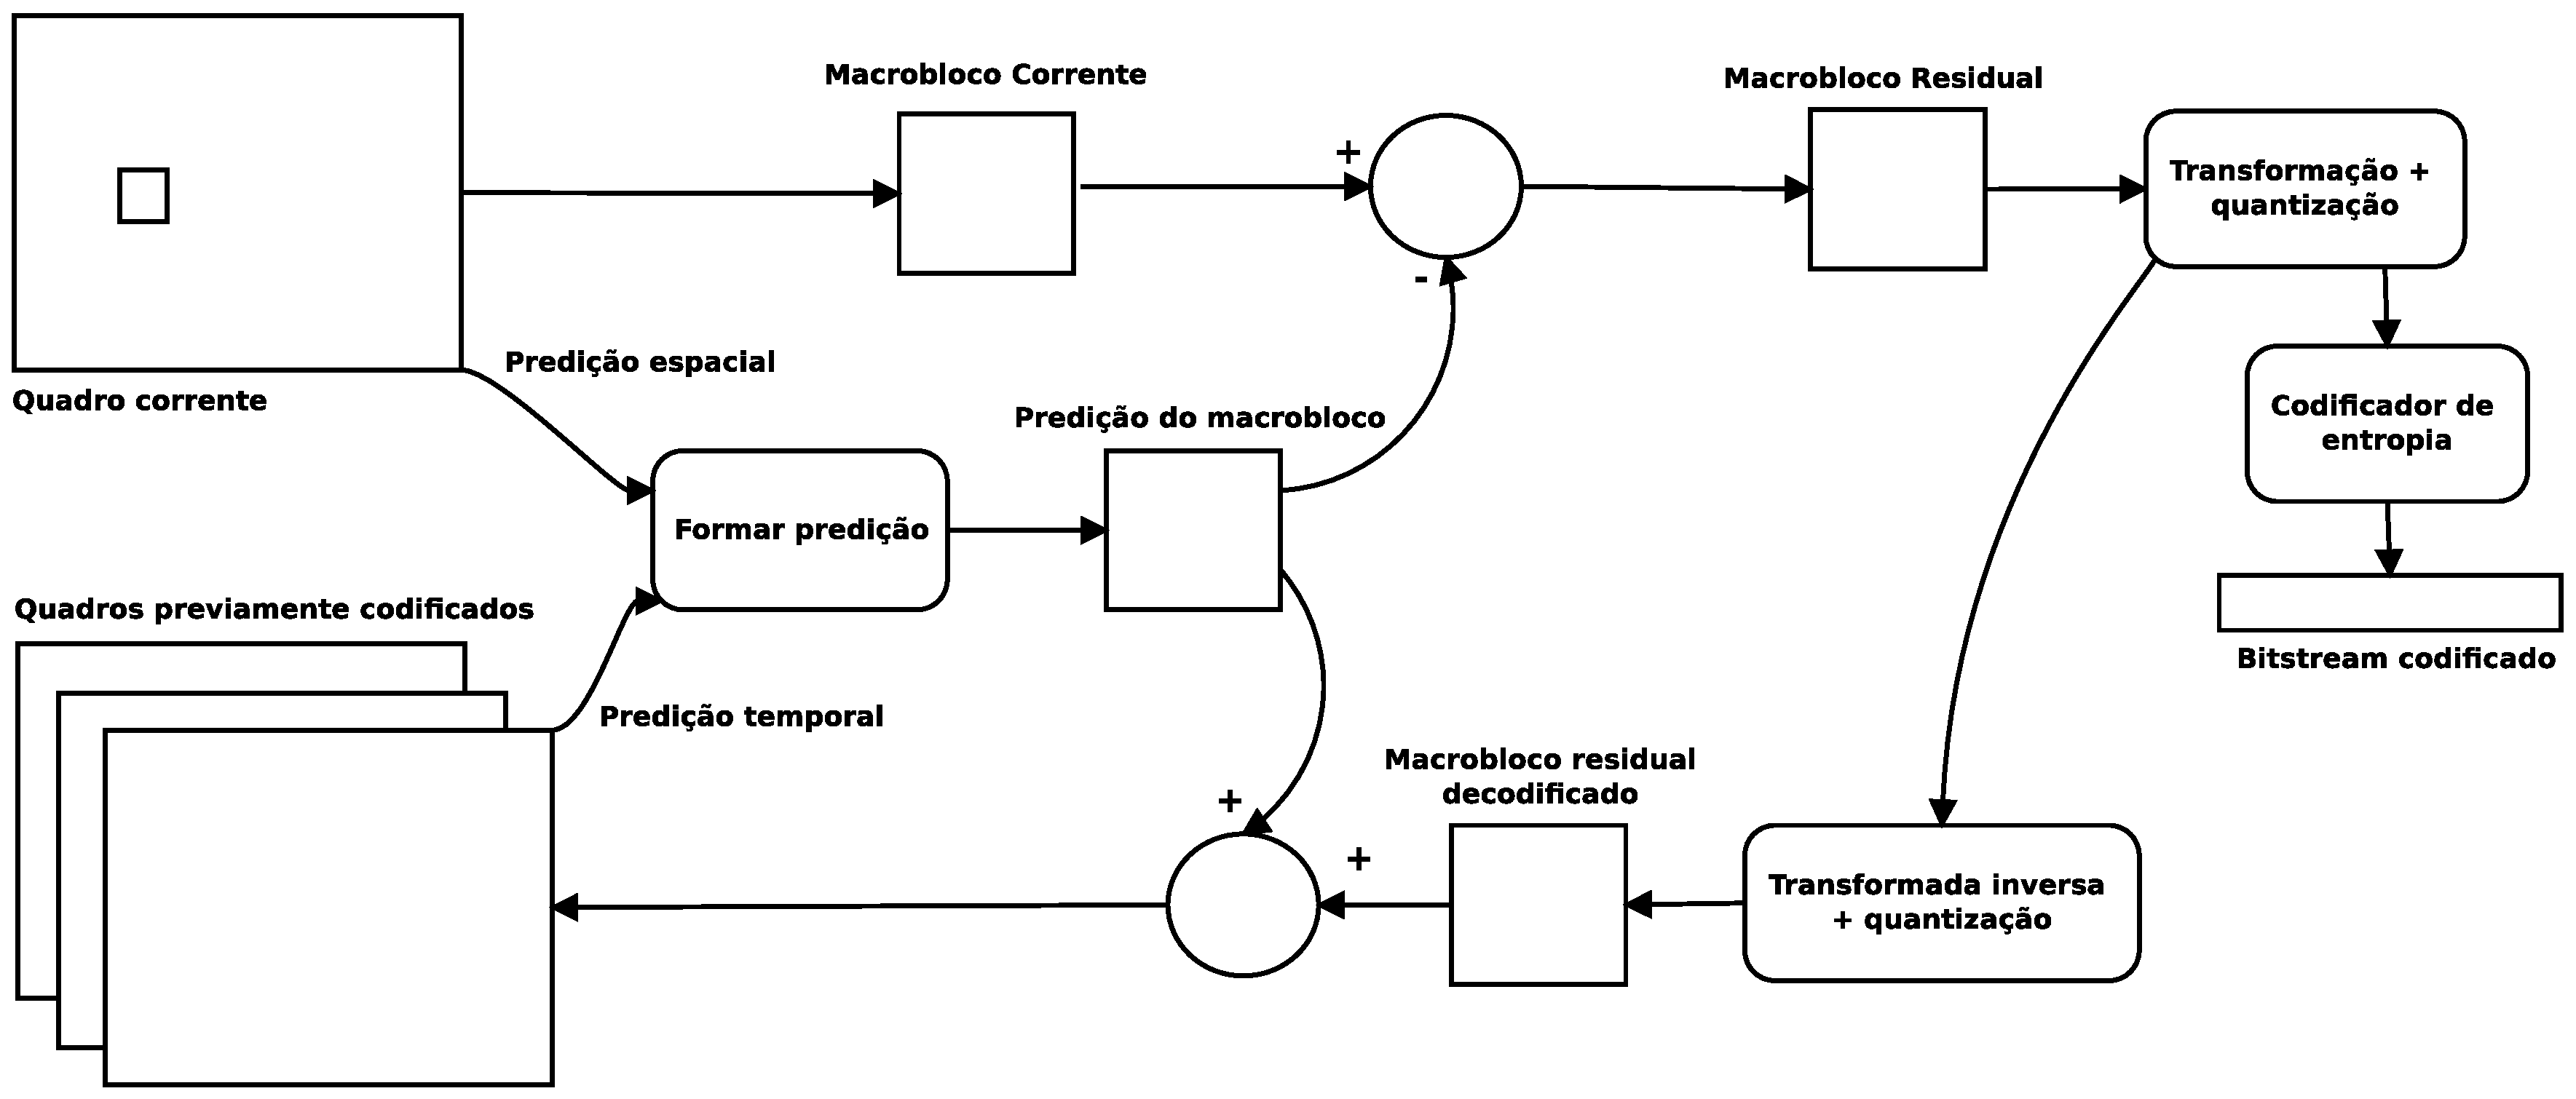
\includegraphics[scale=0.3]{imagens/fig1.eps}
\caption{Típico codificador H.264}
\label{fig:h264_encoder}
\end{figure}


\begin{figure}[H]
\centering
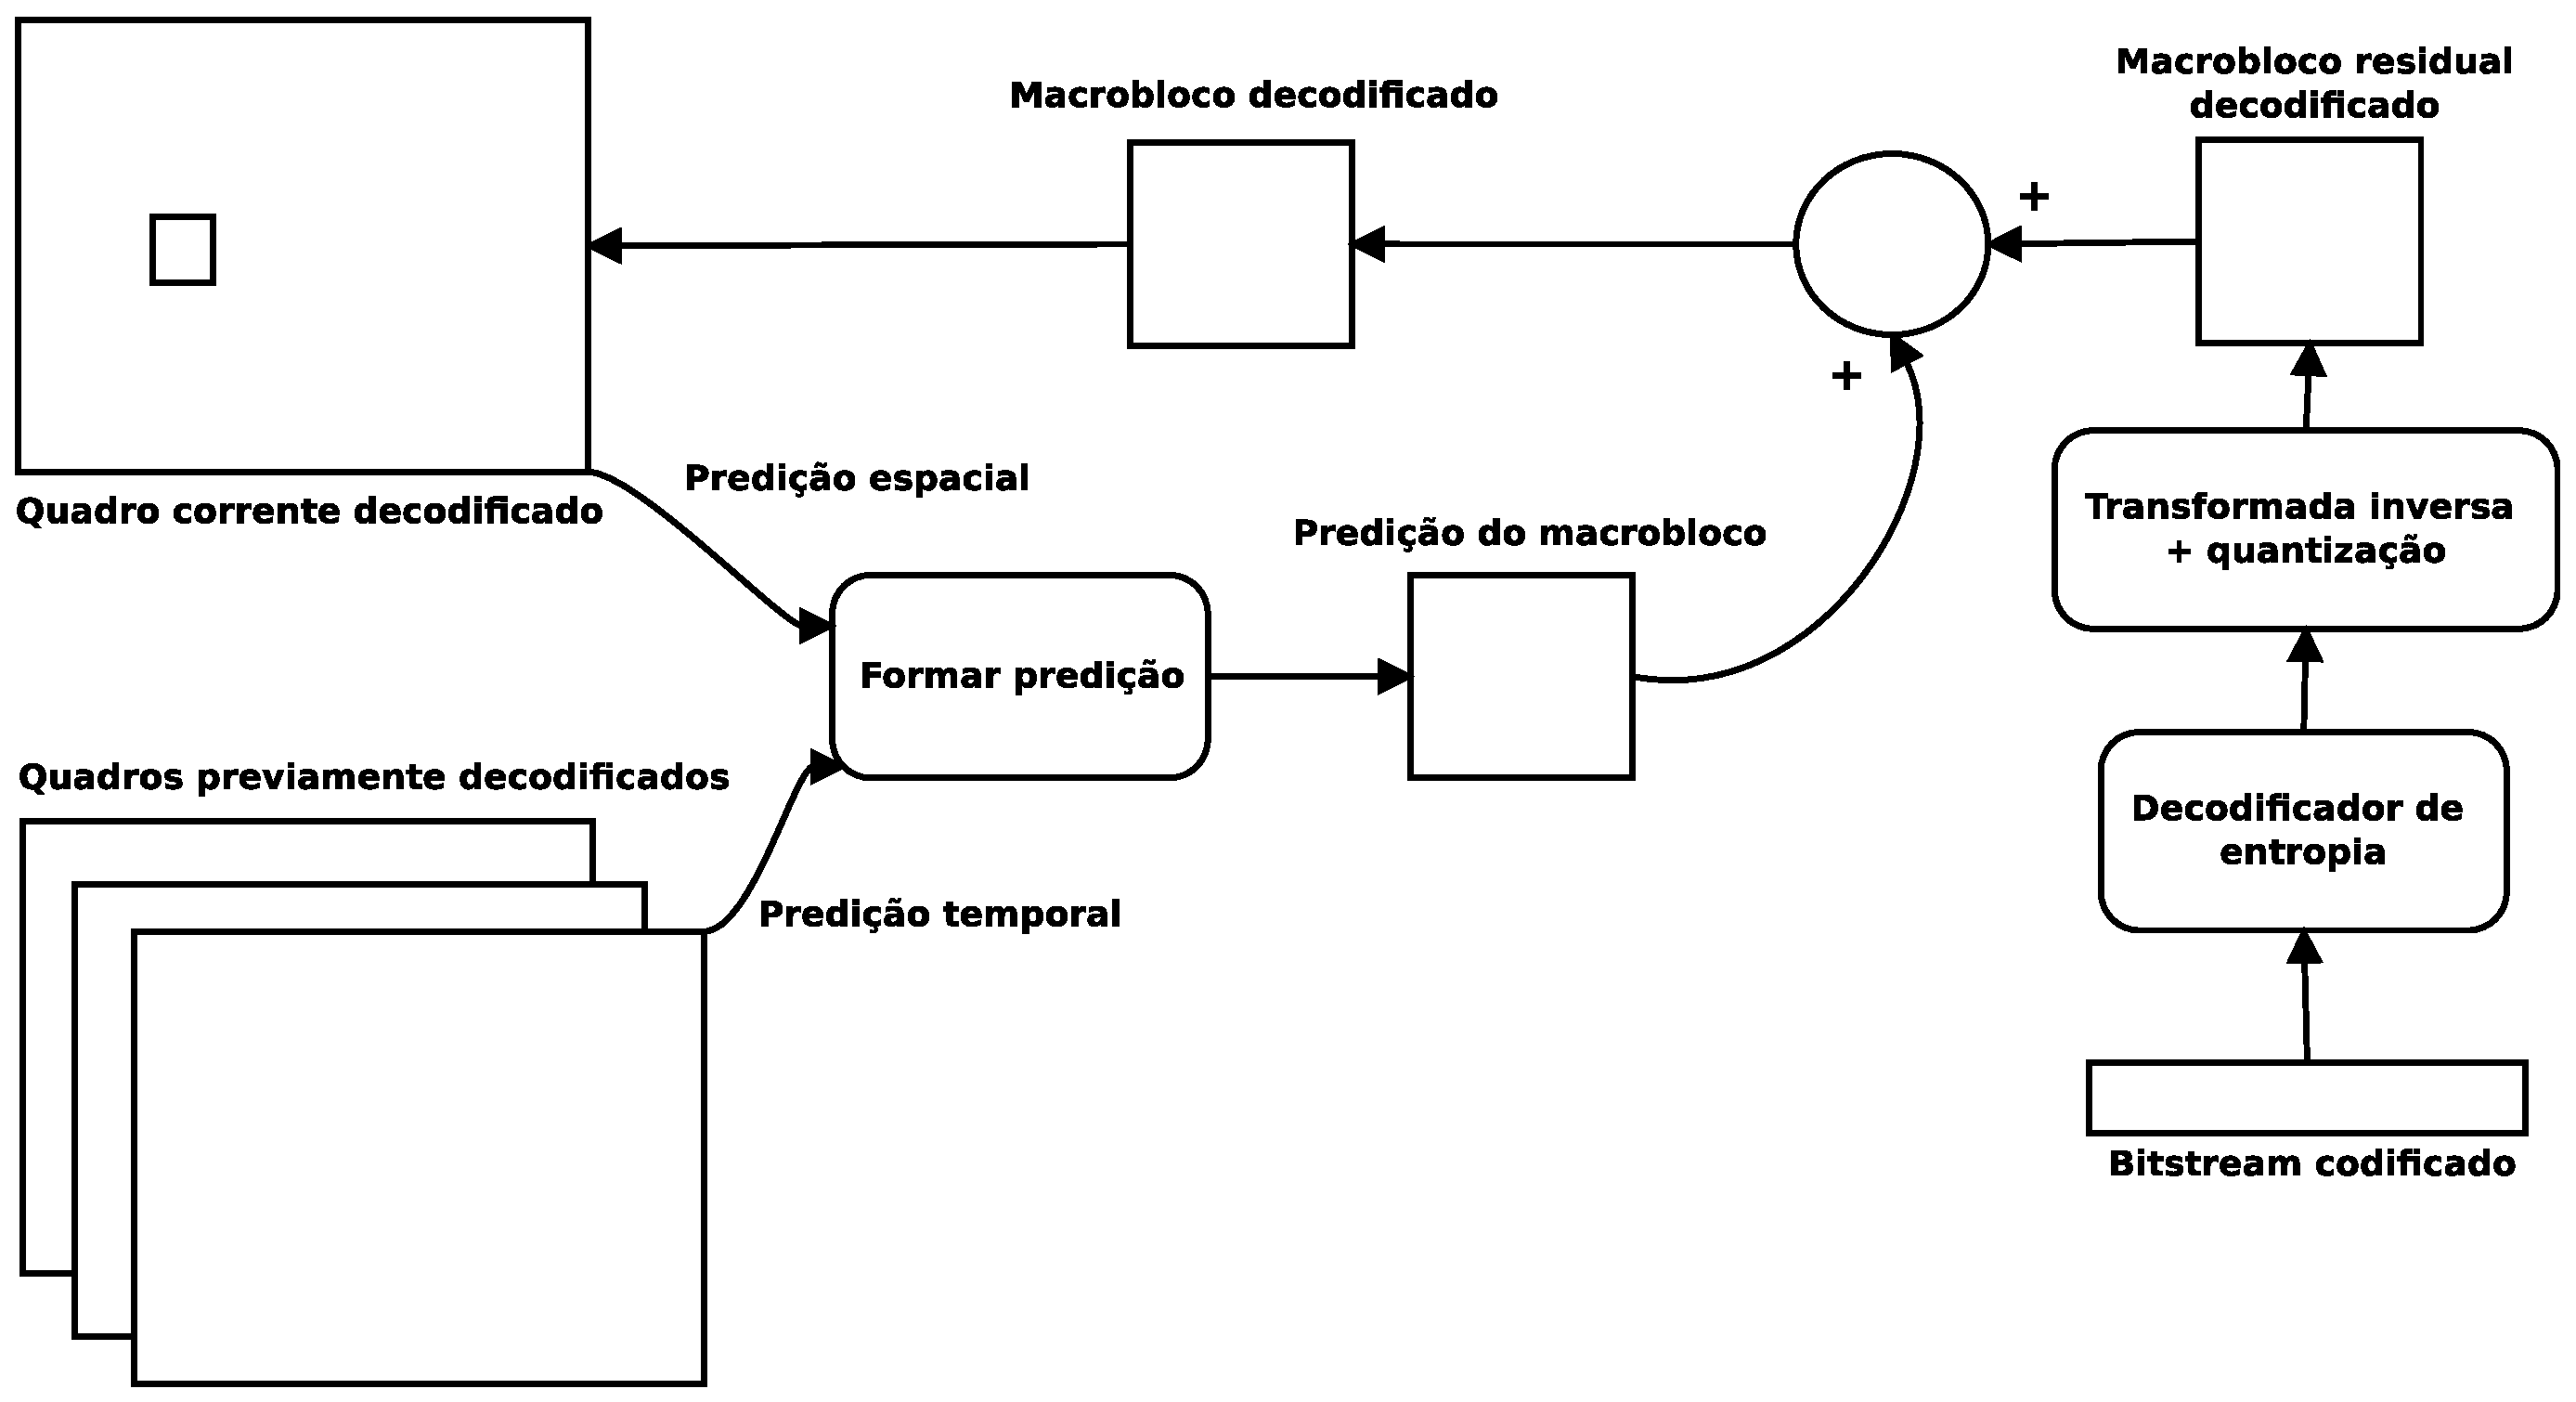
\includegraphics[scale=0.3]{imagens/fig2.eps}
\caption{Típico decodificador H.264}
\label{fig:h264_decoder}
\end{figure}


Todas as informações produzidas pelo codificador tem de ser codificadas e comprimidas em um bitstream que possa ser armazenado/transmitido para ser decodificado posteriormente. Essas informações incluem:

\begin{itemize}
        \item Coeficientes gerados pela transformação (quantizados).
        \item Informação que habilita o decoder a recriar a predição.
        \item Informação da estrutura dos dados comprimidos, e das ferramentas de compressão utilizadas no processo de codificação.
        \item Informação a respeito da sequência de vídeo como um todo.
\end{itemize}

Esses valores e parâmetros, também conhecidos como elementos de sintaxe, são convertidos em código binário utilizando codificação de tamanho variado (VLC) e/ou codificação aritmética. Cada um desses métodos produz uma representação binária eficiente e compacta das informações.


\subsection{Sintaxe Geral}


H.264 provê uma sintaxe clara de como representar o vídeo comprimido e informações relacionadas ao vídeo, essa sintaxe é hierárquica. No nível mais alto, uma sequência H.264 consiste de uma série de "pacotes" ou Network Abstraction Layer Units (NALUs). 

Um NALU (Network Abstraction Layer Unit) contem um RBSP (Raw Byte Sequence Payload), que é uma sequência de bytes contendo os elementos da sintaxe. No H.264 os elementos da sintaxe são códigos binários de tamanho variado, portanto uma sequência de elementos de sintaxe dentro de um NALU não vai necessariamente encaixar em um número integral de bytes, bits com valor zero são adicionados ao final do RBSP para garantir isso.

Cada NALU consiste de um cabeçalho de 1 byte, seguido de um stream de bytes contendo informações de controle ou vídeo codificado. O cabeçalho indica o tipo do NALU e a "importância" dele. NALUs utilizados como referência, por exemplo na predição de quadros futuros, são considerados como de alta prioridade, já que a perda de um desses poderia dificultar o processo de decodificação. Já os NALUs que não são utilizados como referência são considerados como tendo uma prioridade mais baixa. Esse tipo de informação pode ser utilizada para priorizar os NALUs mais importantes no momento da transmissão.


\begin{figure}[H]
\centering
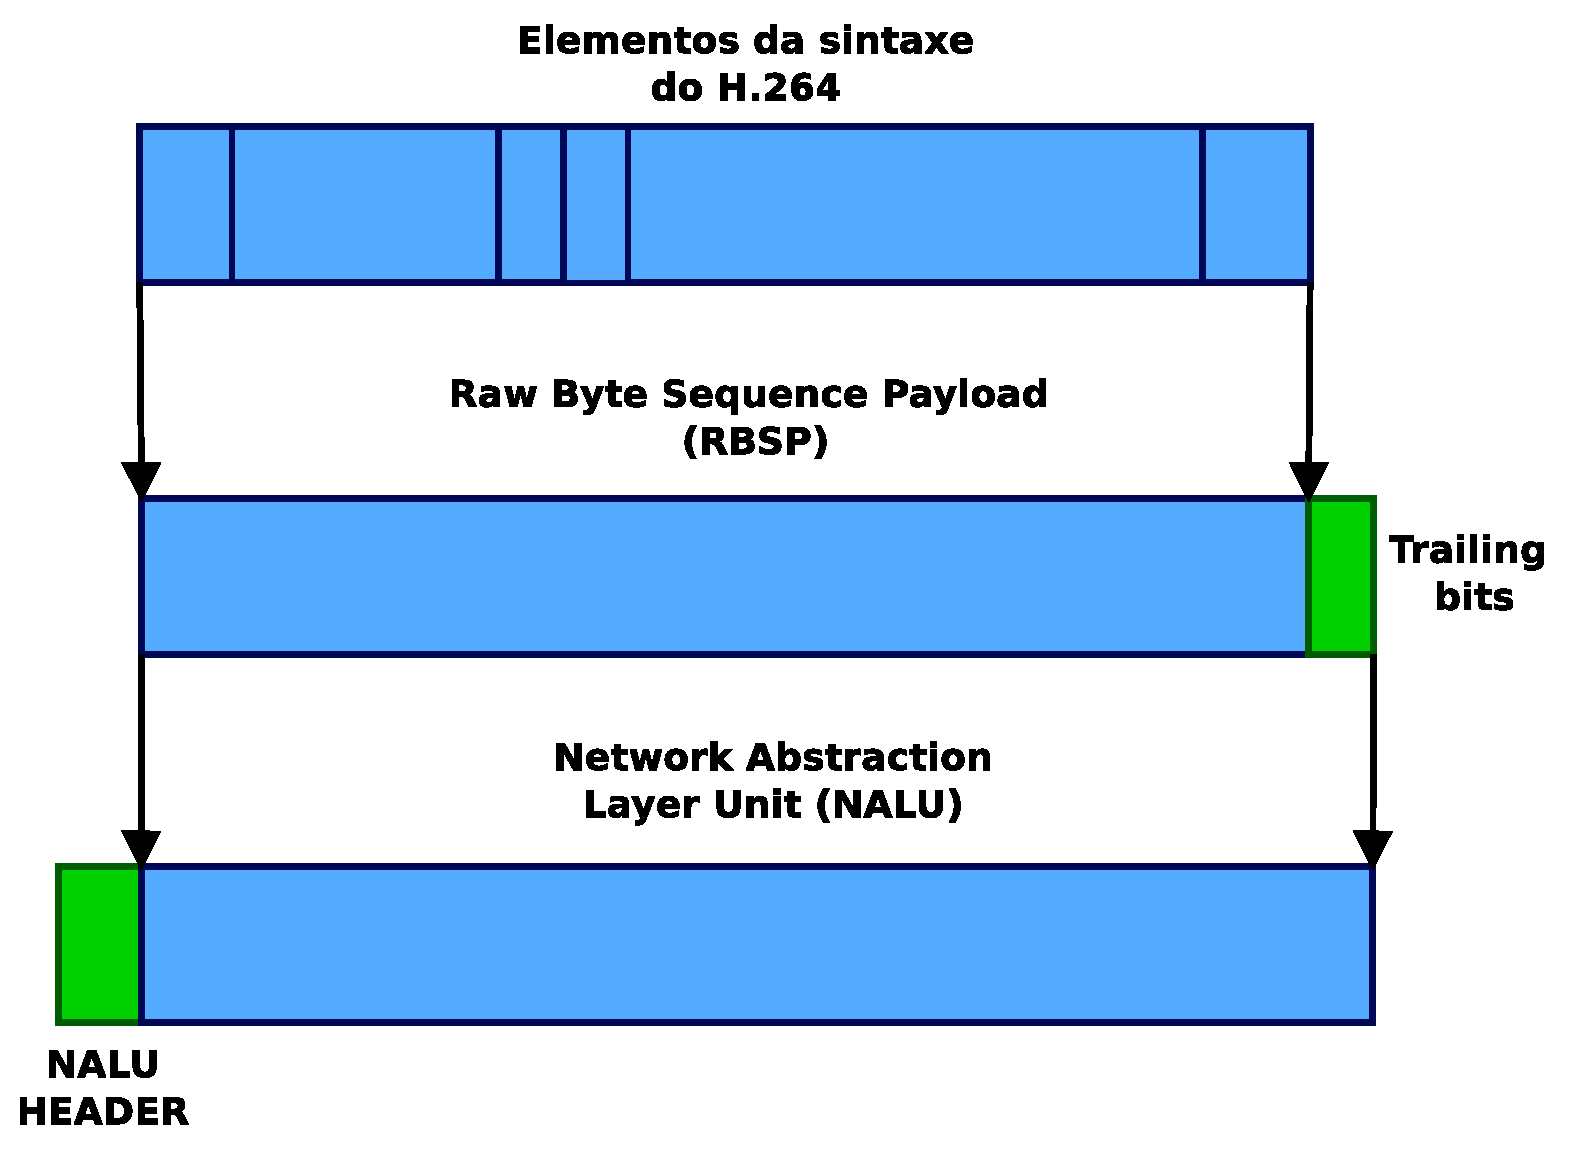
\includegraphics[scale=0.4]{imagens/fig3.eps}
\caption{Encapsulamento de elementos de sintaxe do H.264 em um NALU}
\label{fig:h264_syntax}
\end{figure}


De acordo com \cite{ieeeVideoVol13N7} página 563, um NALU pode ser transmitido usando um protocolo de transporte, onde cada NALU se torna o payload do pacote (orientado a pacote), ou em um stream de bytes, onde cada NALU será transmitido sequencialmente em uma série de bytes (orientado a byte stream), utilizando como prefixo um código de inicio (start code) de 3 bytes indicando que está começando um novo NALU no bitstream. 

Sempre que ocorre de uma sequência de 3 bytes ser similar ao start code, é inserido um emulation prevention byte para prevenir que o decoder confunda essa sequência de bytes com um start code. Quando se utiliza orientação a pacote é desnecessária a utilização do start code e do emulation prevention byte. A sintaxe completa de um NALU pode ser encontrada em \cite{ituh264avc} seção 7.3.1 e sua semântica na seção 7.4.1.


\begin{figure}[H]
\centering
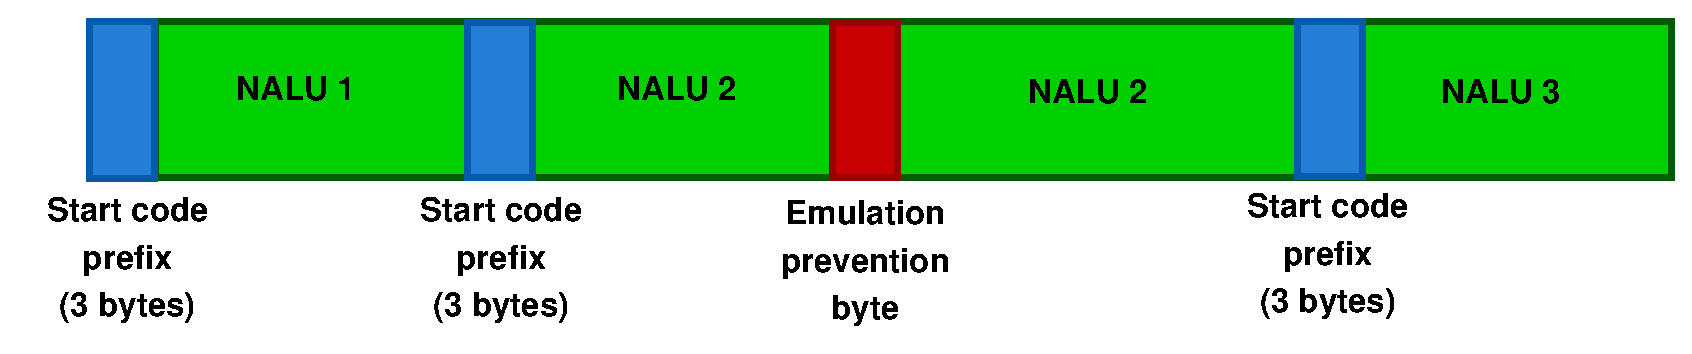
\includegraphics[scale=0.4]{imagens/fig5.eps}
\caption{Exemplo de 3 NALUs sendo transmitidos/armazenados com orientação a bitstream}
\label{fig:h264_nalu_bitstream}
\end{figure}


\begin{figure}[H]
\centering
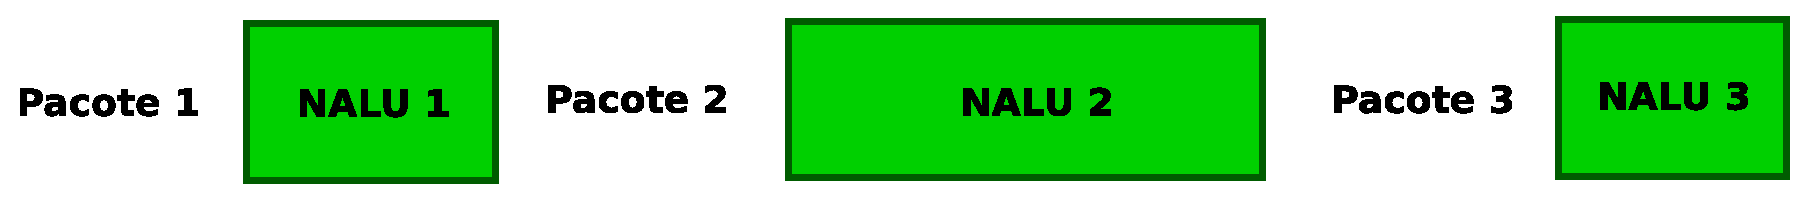
\includegraphics[scale=0.4]{imagens/fig6.eps}
\caption{Exemplo de 3 NALUs sendo transmitidos/armazenados com orientação a pacotes}
\label{fig:h264_nalu_packet}
\end{figure}


Como consta em \cite{ieeeVideoVol13N7} página 564, NALUs podem ser classificados como VCL (pertencem ao video coding layer) ou não-VCL NALUs (não pertencem a Video Coding Layer). 

NALUs VCL possuem as amostras de vídeo (slices) enquanto que NALUs não-VCL possuem informações adicionais associadas ao vídeo como parâmetros (Parameter Sets) que fornecem informações de controle ao decodificador ou SEI (Supplemental Enhancement Information). 

Os Parameter Sets existentes são os SPS (Sequence Parameter Sets), que podem ser aplicados a uma inteira sequência de vídeo, e os PPS (Picture Parameter Sets) que são aplicáveis somente a um ou mais quadros de uma determinada sequência, mas não todos. 


\begin{figure}[H]
\centering
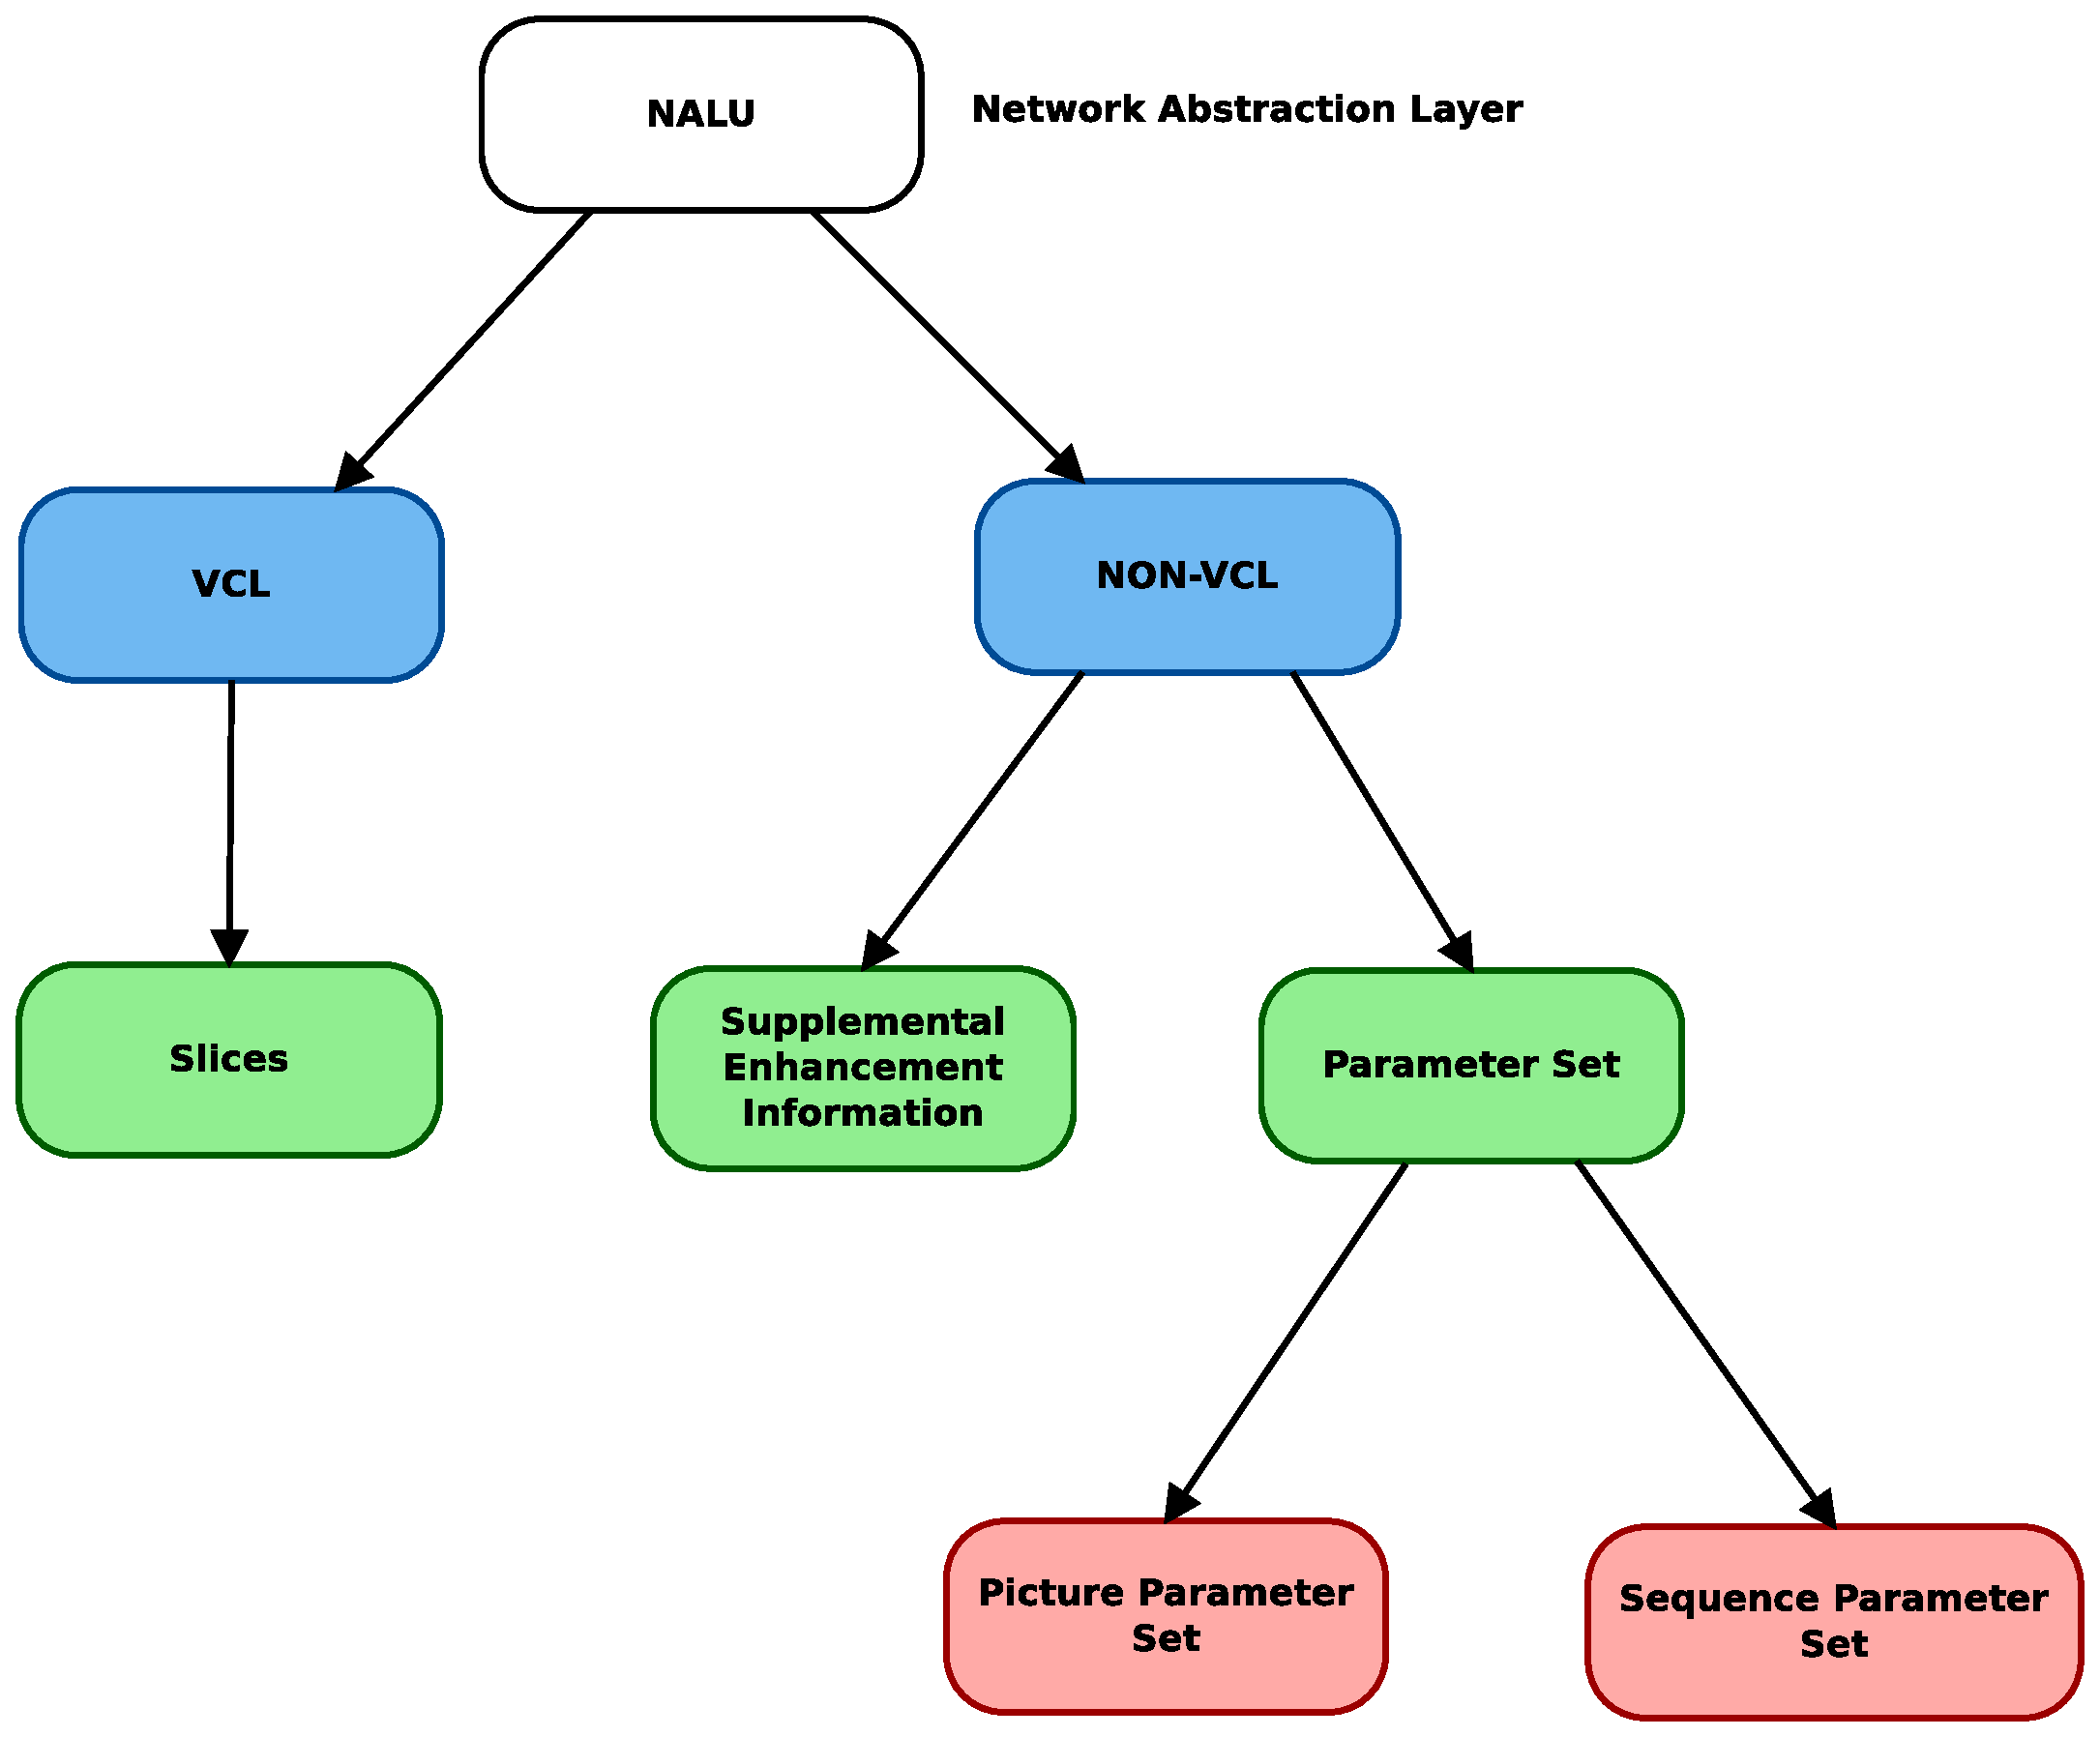
\includegraphics[scale=0.4]{imagens/fig7.eps}
\caption{Possíveis classificações de um NALU}
\label{fig:vcl_nonvcl}
\end{figure}


\subsection{Supplemental Enhancement Information}

Como consta em \cite{ituh264avc} cláusula 7.4.2.3, SEI (Supplemental Enhancement Information) NALUs contêm informações que não são essenciais ao processo de decodificação mas que podem ser utilizadas para auxiliar a decodificação. Um NALU do tipo SEI pode conter uma ou mais mensagens SEI dentro do seu RBSP. A sub-cláusula 7.3.2.3 define a sintaxe do RBSP de um NALU do tipo SEI, mais informações sobre SEI podem ser encontrados no anexo D da recomendação.


\begin{figure}[H]
\centering
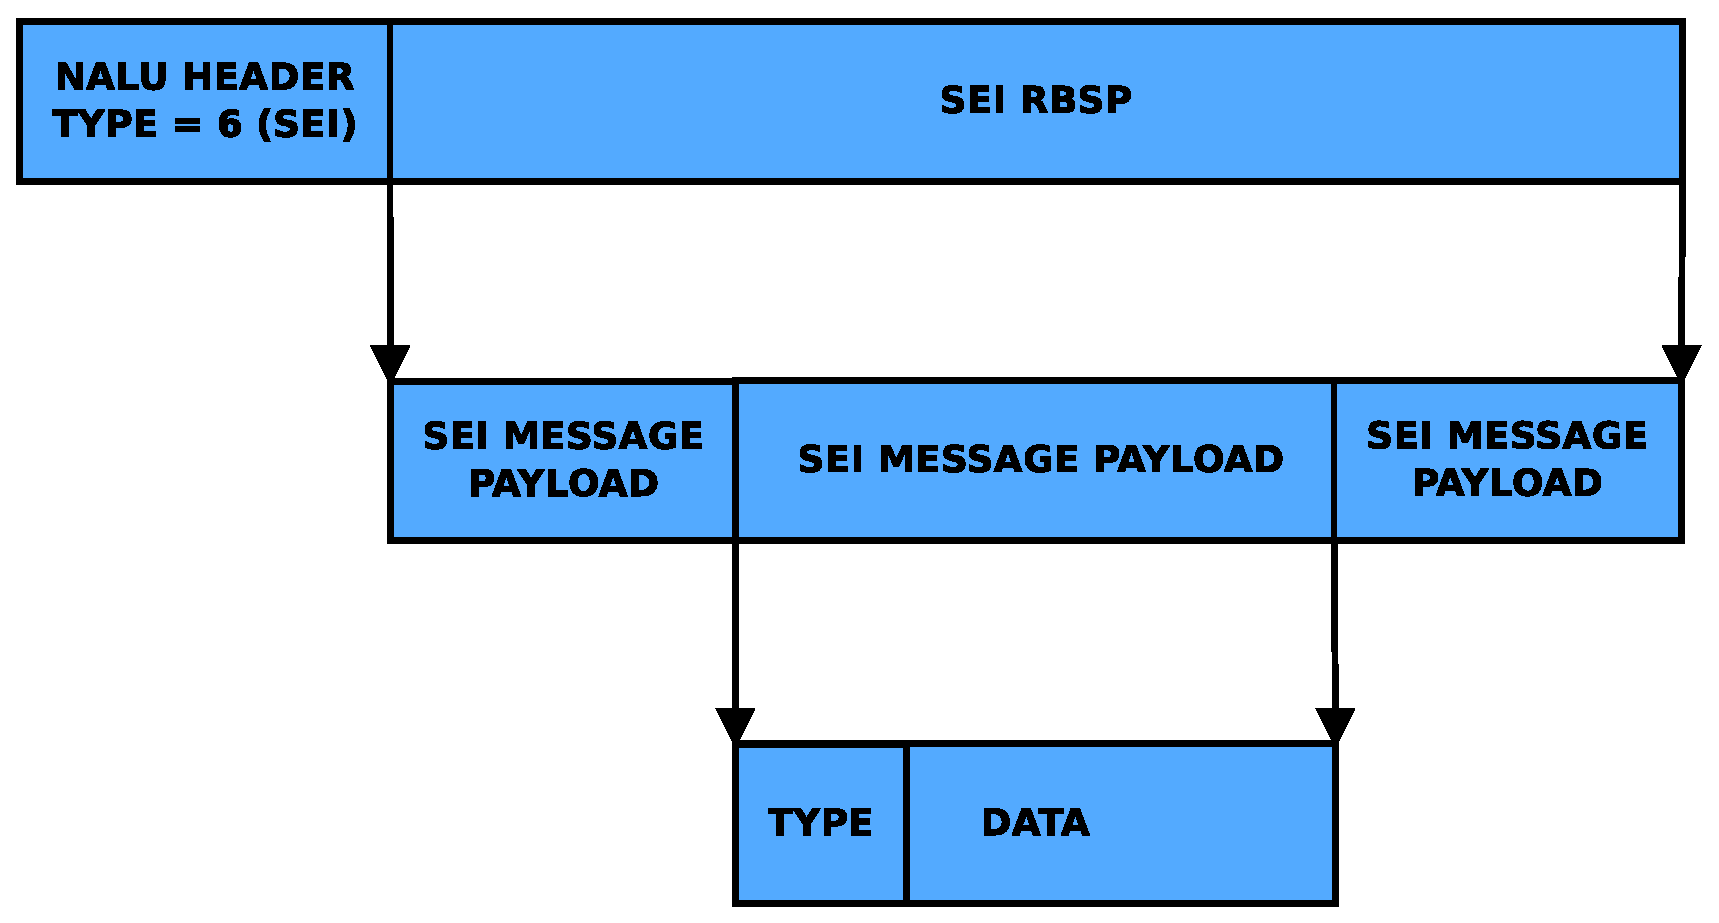
\includegraphics[scale=0.5]{imagens/fig4.eps}
\caption{Exemplo de mensagens SEI encapsuladas em um SEI NALU}
\label{fig:sei_nalu}
\end{figure}


Não existe um limite máximo no tamanho de um SEI NALU, porém existem algumas limitações de buffer que podem resultar em um limite implícito no tamanho do SEI NALU (tabela A.1 do anexo A da \cite{ituh264avc} traz os limites que podem existir de acordo com o nível/perfil que o codificador implemente).

A sub-cláusula 7.3.2.3.1 da recomendação \cite{ituh264avc} define a sintaxe de uma mensagem SEI e a sub-cláusula 7.4.2.3.1 define a sua semântica, nestas sub-cláusulas pode se encontrar informações mais detalhadas de como o decodificador consegue obter o tamanho das mensagens SEI.

Uma mensagem SEI é composta basicamente do tipo do payload e o próprio payload. Normalmente as mensagens SEI são utilizadas para auxiliar o processo de decodificação, por isso existem vários tipos de mensagens pré-definidas. 

Existem dois tipos de mensagem SEI \textit{UserData}, a registrada e a não registrada, ambas podem possuir dados que não são definidos na recomendação \cite{ituh264avc}. Na mensagem SEI \textit{UserData} registrada a mensagem deve ser precedida por um código registrado na ITU-T e a mensagem deve seguir a sintaxe e a semântica estipuladas por esse código informado. 

Já a mensagem SEI \textit{UserData} não registrada necessita de um UUID precedendo a mensagem e o conteúdo da mensagem não precisa obedecer nenhuma sintaxe ou semântica específica. A sintaxe do payload de uma mensagem SEI \textit{UserData} não registrada pode ser encontrada em \cite{ituh264avc} na seção D.1.6 e a definição semântica na seção D.2.6.

Uma lista completa de todos os tipos de mensagens SEI se encontra em \cite{ituh264avc} na seção D.1.


\subsection{Software de referência H.264/AVC}

O software de referência utilizado no presente projeto é desenvolvido pelo JVT (Joint Video Team) e hospedado pelo Instituto Fraunhofer para telecomunicações, Instituto Heinrich Hertz. Esta implementação será utilizada por ela ser referência para pesquisas e verificação de conformidade com a norma. 

A versão utilizada é a 17.2, o download da mesma pode ser realizado gratuitamente em http://iphome.hhi.de/suehring/tml/download, todos os módulos são bem divididos e possuem boa documentação. O software consiste basicamente de um codificador (\textit{lencod}) que codifica um arquivo de vídeo raw para o formato H.264 e de um decodificador (\textit{ldecod}) que decodifica um arquivo H.264 em um arquivo de vídeo raw. Algumas funções de uso comum se encontram no módulo \textit{lcommon}.


\section{Classificador Haar - OpenCV}


\subsection{Introdução}

OpenCV inclui diversas implementações de algoritmos de aprendizagem de máquina (uma lista completa dos algoritmos disponíveis encontra-se em \cite{learningOpenCV} páginas 462 e 463), que é um sub-campo da inteligência artificial que visa transformar dados brutos em informação, tornando possível que a máquina responda a perguntas como: Que outra informação é similar a esta? Existe um carro nessa imagem?

Um desses algoritmos de aprendizagem de máquina é o classificador Haar, esse algoritmo é uma implementação da técnica conhecida como detector Viola-Jones \cite{rapidObjectDetectionViola01} e que depois foi estendido por Rainer Lienhart e Jochen Maydt \cite{extendedSetHaarFeatures02} para utilizar recursos diagonais. Ele é um classificador supervisionado (para mais informações sobre tipos de classificadores veja \cite{learningOpenCV} páginas 460 e 461), ou seja, após treiná-lo é necessário apenas fornecer a imagem ao classificador e ele irá rotular ela como contendo ou não contendo o objeto de interesse.


\subsection{Teoria do classificador Viola-Jones}

O detector Viola-Jones utiliza uma forma de AdaBoost (\cite{learningOpenCV} página 497) mas o organiza como uma cascata de nodos, onde cada nodo desse é um classificador "Multitree AdaBoosted", desenvolvido para ter uma alta (digamos 99,9\%) taxa de detecção (poucos falsos negativos), ás custas de uma baixa (perto de 50\%) taxa de rejeição (grande quantidade de falsos positivos).

A cascata de nodos funciona como uma cascata de rejeição, para cada nodo na cascata, um "não pertence a classe" encerra a computação e o algoritmo responderá que não existe o objeto de pesquisa na região determinada para busca.  A região só é classificada como possuindo um objeto de determinada classe se a computação ocorrer com sucesso por toda a cascata. 

Em casos onde o objeto de interesse é raro (por exemplo uma face em uma foto), cascatas de rejeição aceleram o processo de busca por um objeto, já que a maior parte das regiões de busca será marcada como não possuindo o objeto rapidamente, sem ter de percorrer a maior parte da cascata. Em cada nodo da cascata de rejeição existe um conjunto de classificadores fracos, que são árvores de decisão. O conjunto de árvores em cada nodo é acelerado com a técnica de Boosting (mais informações sobre a técnica de Boosting podem ser encontradas em \cite{learningOpenCV} página 495).

 Essas árvores normalmente possuem profundidade um, sendo também chamadas de \textit{decision stumps}, são o caso mais simples de árvores de decisão o qual consiste de um único nodo de decisão e duas folhas. Cada "decision stump" deve tomar apenas uma decisão, da seguinte forma: "Está o valor V de um determinado recurso R acima ou abaixo de um limite L"; Nesse caso um "sim" indica que o objeto de interesse está presente, um "não" indica a sua ausência.

\begin{displaymath}
   f{i} = \left\{
     \begin{array}{lr}
       +1 & : V{i} \geq T{i} \\
       -1 & : V{i} < T{i} 
     \end{array}
   \right.
\end{displaymath}

A quantidade de recursos Haar que o classificador Viola-Jones utiliza em cada classificador fraco pode ser configurado no momento do treinamento, normalmente se utiliza apenas um recurso (uma árvore com apenas uma divisão) ou no máximo 3 recursos. Incrementar esses classificadores iterativamente (técnica de Boosting) constrói um classificador que é a soma ponderada dos classificadores fracos. O classificador Viola-Jones usa a seguinte função de classificação:

\begin{equation}
F = sinal(w{1}f{1} + w{2}f{2} + ... + w{n}f{n})
\end{equation}

A função sinal retorna -1 se o resultado da soma for menor ou igual a 0,0, do contrário retorna +1. Ao analisar pela primeira vez o conjunto de dados, nós aprendemos o limite l1 de f1 que melhor classifica a entrada. A técnica de Boosting utiliza os erros para realizar o calculo ponderado de w1. Cada vetor de recursos é reavaliado como tendo menos peso (se ele foi classificado corretamente) ou mais peso (se ele foi classificado incorretamente). 

Pode parecer estranho diminuir o peso do vetor de dados quando ele é classificado corretamente, e aumentar o peso quando a classificação falha. A razão do treinamento ocorrer assim é que a técnica de Boosting tem como objetivo corrigir os pontos onde existem "problemas" e ignorar os pontos que já funcionam bem. Depois que o nodo é ensinado, os dados sobreviventes da parte superior da cascata são usados para treinar o próximo nodo, e assim por diante.

Um detalhe importante é o uso de recursos Haar como entrada do algoritmo, em vez de dados brutos. Esses recursos Haar são basicamente um limite aplicado às somas e diferenças de regiões retangulares da imagem. Para acelerar o cálculo desses recursos é utilizada a técnica de imagem integral (para mais detalhes veja \cite{learningOpenCV} página 182) que acelera o cálculo do valor de regiões retangulares e dessas mesmas regiões rotacionadas em 45 graus. 

Viola e Jones organizaram cada grupo classificador boosted em nodos, formando uma cascata de rejeição, como mostrado na figura ~\ref{fig:cascata_rejeicao_haar}. Na figura , cada nodo F contem uma inteira cascata boosted de grupos de \textit{decision stumps} (ou árvores) treinadas utilizando recursos Haar. Normalmente os nodos são ordenados do menos complexo ao mais complexo, assim o custo computacional é minimizado (os nodos mais simples são executados primeiro) ao analisar regiões da imagem que com certeza não possuem o objeto de interesse.

\begin{figure}[H]
\centering
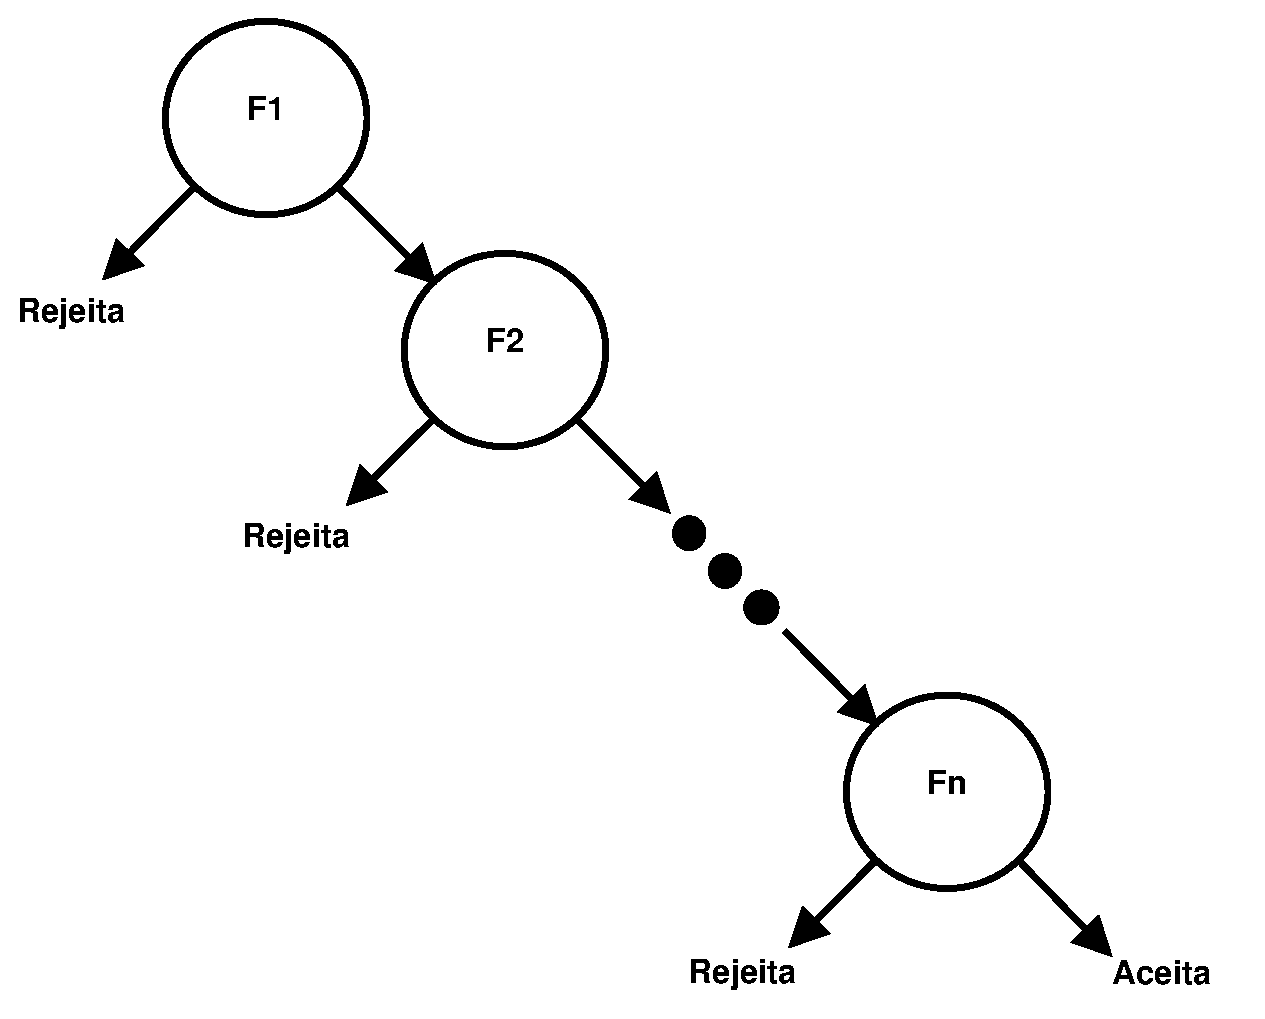
\includegraphics[scale=0.6]{imagens/fig8.eps}
\caption{Cascata de rejeição utilizada no classificador Viola-Jones: Cada nodo representa um classificador "Multitree AdaBoosted" treinado para raramente perder o objeto de interesse, rejeitando porém apenas uma pequena parte das regiões que não representam o objeto de interesse. Até chegar o final da cascata a maior parte das regiões que não representam o objeto de interesse já foram descartadas. }
\label{fig:cascata_rejeicao_haar}
\end{figure}


\subsection{Uso do classificador}

O classificador Haar funciona bem em objetos como faces frontais, olhos, boca, traseira de carros, lateral de carros, frente de carros; Mas objetos como o perfil de um rosto (ou qualquer outro objeto em que o contorno seja a característica principal de identificação), já não funciona tão bem, principalmente porque essa perspectiva insere variações no padrão que os recursos em forma de bloco do Haar não conseguem lidar muito bem. 

Por exemplo, para modelar a curva de um rosto visto de lado (seu contorno) é necessário inserir no modelo informações a respeito do fundo da imagem, para realizar essa modelagem de maneira adequada seria necessário um conjunto de treinamento muito maior, com diferentes fundos na imagem, ou rostos de lado com fundos diferentes do modelado seriam rejeitados. Ou seja, o contorno de um objeto é difícil de modelar nesse classificador porque os recursos Haar funcionam em bloco, dessa maneira o classificador é obrigado a aprender as variações do fundo da imagem que formam a borda do objeto.

Para treinar o classificador é necessário ter um grande conjunto de dados, com boa qualidade, bem segmentado, para detecção de objetos rígidos onde o contorno não é a principal característica do objeto. O treinamento desse classificador é lento, porém graças a modelagem em cascata de rejeição ele é bem rápido para realizar a detecção do objeto em si.

Por grande conjunto de dados entende-se milhares de imagens com o objeto de interesse e dezenas de milhares de objetos sem o objeto de interesse. Por boa qualidade dos dados entende-se que os dados não devem conter o mesmo objeto em perspectivas diferentes, para cada perspectiva diferente é melhor treinar um classificador especifíco para aquela perspectiva. 

Por bem segmentado entende-se imagens que representam corretamente o objeto sem variações desnecessárias, isso faria com que o classificador corrigisse essa variação fictícia, levando a resultados imprecisos. Por exemplo, ao treinar o classificador para detectar faces frontais, se a localização dos olhos no rosto variar demais (algo fora do normal) o classificador vai assumir que a localização dos olhos não é fixa e que é normal que os olhos possam estar em qualquer posição, isso degrada muito o desempenho já que o classificador precisa se ajustar a fatores que não existem nos dados reais.


\chapter{Projeto}


Este capítulo descreve o desenvolvimento prático do projeto, que é composto da detecção e \textit{tracking} de objetos dentro do software de referência, da utilização dos vetores calculados na estimativa de movimento para auxiliar no \textit{tracking} de objetos e da inserção dos metadados extraídos no bitstream. Primeiro são apresentados resultados práticos da inserção de mensagens \textit{SEI Userdata Unregistered} no bitstream de um vídeo codificado. Em seguida serão apresentados os novos módulos adicionados para realizar a extração e o armazenamento dos metadados e como eles foram integrados ao software de referência. Por fim será apresentada uma avaliação dos resultados obtidos.


\section{Inserindo userdata no Bitstream}


O H.264 possui uma sintaxe específica para o envio de mensagens não necessárias ao processo de decodificação, embutidas no bitstream de vídeo, são mensagens SEI (\textit{Supplemental Enhanced Information}). Ao longo dessa seção será estudada a utilização prática das mensagens SEI do tipo \textit{UserData} não registrada em pontos diferentes no processo de codificação. 


\subsection{Ambiente de teste}

Todos os testes foram realizados com o mesmo trecho de vídeo obtido a partir do site http://media.xiph.org/video/derf.

O vídeo possui a seguinte configuração:

\begin{itemize}
        \item quadros por segundo = 29.97.
        \item total de quadros    = 300.
        \item comprimento         = 176 pixels.
        \item altura              = 144 pixels.
        \item espaço de cor       = YUV, 4:2:0.
\end{itemize}

Para testar a conformidade do bitstream gerado foi utilizado o decodificador de referência, após utilizar o decodificador de referência para transformar o bitstream H.264 em vídeo raw foi utilizado o Gstreamer para exibir o vídeo e constatar visualmente que o vídeo foi decodificado sem problemas.

O bitstream também foi testado diretamente no Gstreamer, pra verificar se o bitstream tocaria em um player usual (muitos players open source utilizam gstreamer como framework de multimedia). 

Gstreamer utiliza internamente o ffmpeg para fazer o decoding do bitstream H.264. 


\subsection{Enviando uma mensagem SEI Userdata}

Inicialmente foi utilizada a opção \textit{GenerateSEIMessage} do próprio codificador, onde é possível ativar o envio de uma mensagem e configurar a mensagem que será enviada. Mas isso serve apenas para testes bem simples já que apenas uma mensagem é enviada ao longo de todo o bitstream de vídeo, e em forma de texto. Essa função é invocada no módulo \textit{filehandle}, por isso ele foi escolhido como ponto de partida para testes de inserção de mensagens SEI no bitstream.

A partir do que foi observado na presente implementação de envio de mensagens SEI não registradas foi desenvolvida uma nova função que consegue criar uma mensagem SEI com qualquer tipo de dado, não sendo necessariamente texto. Para testar essa nova função foram feitas pequenas alterações no módulo filehandle do codificador, na função \textit{start\_sequence}, e foi adicionado um novo módulo \textit{udata\_gen} para possibilitar a criação de mensagens SEI a partir de um char* e do seu tamanho.

Também foram realizadas alterações no decodificador para realizar a extração da mensagem SEI, para isso foi criado um novo módulo \textit{udata\_parser} que faz a extração dos dados a partir de um SEI NALU que possui uma mensagem SEI do tipo \textit{UserData} não registrada.

O módulo \textit{udata\_parser} é chamado dentro do módulo sei (\textit{sei.c}) do decodificador (\textit{ldecod}), na função \textit{InterpretSEIMessage} que trata a recepção de mensagens SEI. Nesse ponto as informações são enviadas para o \textit{stdout}, para constatar se as mensagens foram extraídas corretamente.

Com essas duas alterações prontas foi possível testar o envio de um \textit{SEI User Data} não registrado contendo informação que não é necessariamente texto (nesse caso a ideia é que fossem parâmetros extraídos do video). 

Foi constatado que:

\begin{itemize}
        \item As informações persistiram no bitstream e foram extraídas com sucesso pelo decodificador de referência modificado.
        \item O decodifica de referência realizou a decodificação do vídeo com sucesso, gerando um arquivo de vídeo bruto válido com todo o vídeo original.
        \item O bitstream H.264 gerado mostrou ser compatível com Gstreamer.
\end{itemize}

Portanto não seria um problema enviar dados de qualquer natureza utilizando mensagens \textit{SEI User Data} não registradas, o decodificador de referência continuou funcionando sem problemas e a mensagem permaneceu íntegra. Até mesmo um decodificador de terceiro (ffmpeg + Gstreamer) funcionou com o bitstream gerado.


\subsection{Enviando diversas mensagens SEI Userdata de tamanho variado}


Após ter enviado uma mensagem com sucesso o próximo passo foi enviar várias mensagens no mesmo bitstream, com tamanhos variados. Porém surgiram dois problemas, a quantidade de mensagens \textit{SEI Userdata} que podem ser enviadas no mesmo bitstream e o tamanho máximo delas. De acordo com \cite{ituh264avc} não existe um limite explicito nem na quantidade, nem no tamanho das mensagens SEI.

Porém na prática, além dos limites implícitos que podem existir por causa do nível de conformidade do codificador, muitos decodificadores possuem limites no que eles suportam que estão relacionados com a maneira como eles foram implementados e não com a recomendação em si. 

Alguns decodificadores possuem limites de quantas mensagens SEI podem receber, outros simplesmente descartam mensagens SEI. Como a variedade de decodificadores é muito grande, o foco da implementação será o codificador/decodificador de referência.

No codificador de referência existe um limite explicito no tamanho máximo de um NALU, esse limite é definido no arquivo \textit{lcommon/inc/nalucommon.h} como \textit{MAXNALUSIZE}. O valor desse limite é 64000 bytes. Ao longo dos testes esse será o tamanho máximo utilizado.

Para testar o envio de múltiplos SEI NALUS com mensagens \textit{SEI Userdata} de tamanhos variados, respeitando o limite de 64000 bytes, foi criada uma nova função no módulo \textit{udata\_gen} que gera uma \textit{string} maior a cada nova chamada. 

Ao atingir o tamanho limite a função retorna ao tamanho inicial e reinicia o processo de aumento da string. Dessa maneira é possível enviar diversas mensagens todas de tamanho diferente, explorando desde mensagens de tamanho pequeno como de mensagens que cheguem perto do tamanho máximo.

Foi feita uma alteração no módulo \textit{filehandle} do codificador, para criar e escrever no bitstream 1000 mensagens de tamanho variado. Nenhuma alteração foi necessária no decodificador.

Foi constatado que:

\begin{itemize}
        \item Os 1000 SEI NALUs persistiram no bitstream e foram extraídos com sucesso pelo decodificador de referência modificado.
        \item O decodifica de referência realizou a decodificação do vídeo com sucesso, gerando um arquivo de vídeo bruto válido com todo o vídeo original.
        \item O bitstream H.264 gerado com os 1000 SEI NALUS mostrou ser compatível com Gstreamer.
\end{itemize}

Portanto não seria um problema enviar múltiplos SEI NALUs no mesmo bitstream, e de tamanho variado, desde que se respeite o tamanho máximo definido pelo software de referência. A única limitação deste teste é que os SEI NALUs são escritos no bitstream sequencialmente, não estão intercalados com os NALUs de vídeo e são todos escritos no inicio do bitstream, antes dos quadros de vídeo.

Foi realizado um teste para constatar se múltiplos SEI NALUs vão funcionar bem intercalados com quadros de vídeo. Para isso foram utilizadas as mesmas funções já existentes nos testes anteriores, mas ao invés de os SEI NALUs serem inseridos no módulo \textit{filehandle} eles são inseridos no módulo \textit{lencod}, após a geração de cada quadro. 

Como o vídeo consiste em 300 quadros, foram inseridos exatamente 300 SEI NALUs, sempre que um quadro é escrito no bitstream um SEI NALU de tamanho variável é escrito após ele.

Foi constatado que:

\begin{itemize}
        \item Os 300 SEI NALUs persistiram no bitstream e foram extraídos com sucesso pelo decodificador de referência modificado.
        \item O decodificador de referência realizou a decodificação do vídeo com sucesso, gerando um arquivo de vídeo bruto válido com todo o vídeo original.
        \item O bitstream H.264 gerado com os 300 SEI NALUS mostrou ser compatível com Gstreamer.
\end{itemize}

Utilizando mensagens \textit{SEI Userdata} não registradas é possível enviar dados que não fazem parte do processo de decodificação, de tamanhos variados (respeitando o tamanho máximo estipulado pelo software de referência), em posições variadas dentro do bitstream e em quantidades variadas. O código fonte de todos os módulos alterados no software de referência e dos novos módulos, que foram utilizados para realizar esse teste, se encontra no apêndice A.


\section{ Módulo extracted\_metadata }


Esta seção explica detalhadamente a implementação do módulo \textit{extracted\_metadata}. Ele é escrito em linguagem C e foi adicionado no diretório \textit{lcommon} do software de referência já que ele é utilizado tanto pelo codificador como pelo decodificador. Todas as funções são declaradas no cabeçalho \textit{lcommon/inc/extracted\_metadata.h} e implementadas em \textit{lcommon/src/extracted\_metadata.c}.

Apesar de ser escrito em C, foi utilizada uma abordagem orientada a objetos. A orientação a objetos é feita internamente de uma maneira bem simples, a classe pai possui uma lista de ponteiros de função e na construção da classe filho ela fornece a implementação para essas funções.

A classe pai pode realizar alguma atividade antes ou depois da chamada da função implementada pela classe filho. Dessa maneira fica fácil a classe pai executar código que é comum a todas as subclasses, antes de chamar a função implementada pela subclasse. Isso foi especialmente útil na implementação da serialização, cada implementação de metadado deve se preocupar apenas com a serialização dos seus dados, sem se preocupar com os dados da classe pai, já que a classe pai irá serializar esses dados antes de chamar a função de serialização da classe filho, simplificando a implementação de novos metadados.

Funções da família \textit{hton}, definidas em \textit{arpa/inet.h}, foram utilizadas na serialização dos metadados para garantir que ao serializar os dados os bytes estejam de acordo com o padrão para rede. Na desserialização, funções da família \textit{ntoh} foram utilizadas para garantir que os bytes ordenados de acordo com o padrão para rede fossem convertidos para a ordenação de \textit{bytes} do \textit{host}.

O padrão utilizado nos nomes das funções é \textit{nome\_do\_tipo\_método}. Por exemplo a implementação em C do método \textit{new} da classe ExtractedMetadataBuffer será \textit{extracted\_metadata\_buffer\_new}. Por classe entende-se a estrutura definida com o determinado nome, e sempre ao chamar uma função que é método desta classe, o primeiro parâmetro é um ponteiro para a estrutura que representa a classe. Ao longo dessa seção será feita referência apenas ao nome dos métodos, e não ao nome completo da função que está implementada em C.

Na figura ~\ref{fig:extracted_metadata_class_diagram} pode ser visto o diagrama de classe dos objetos definidos no módulo. A descrição de cada um dos objetos são apresentados nessa seção. 


\begin{figure}[H]
\centering
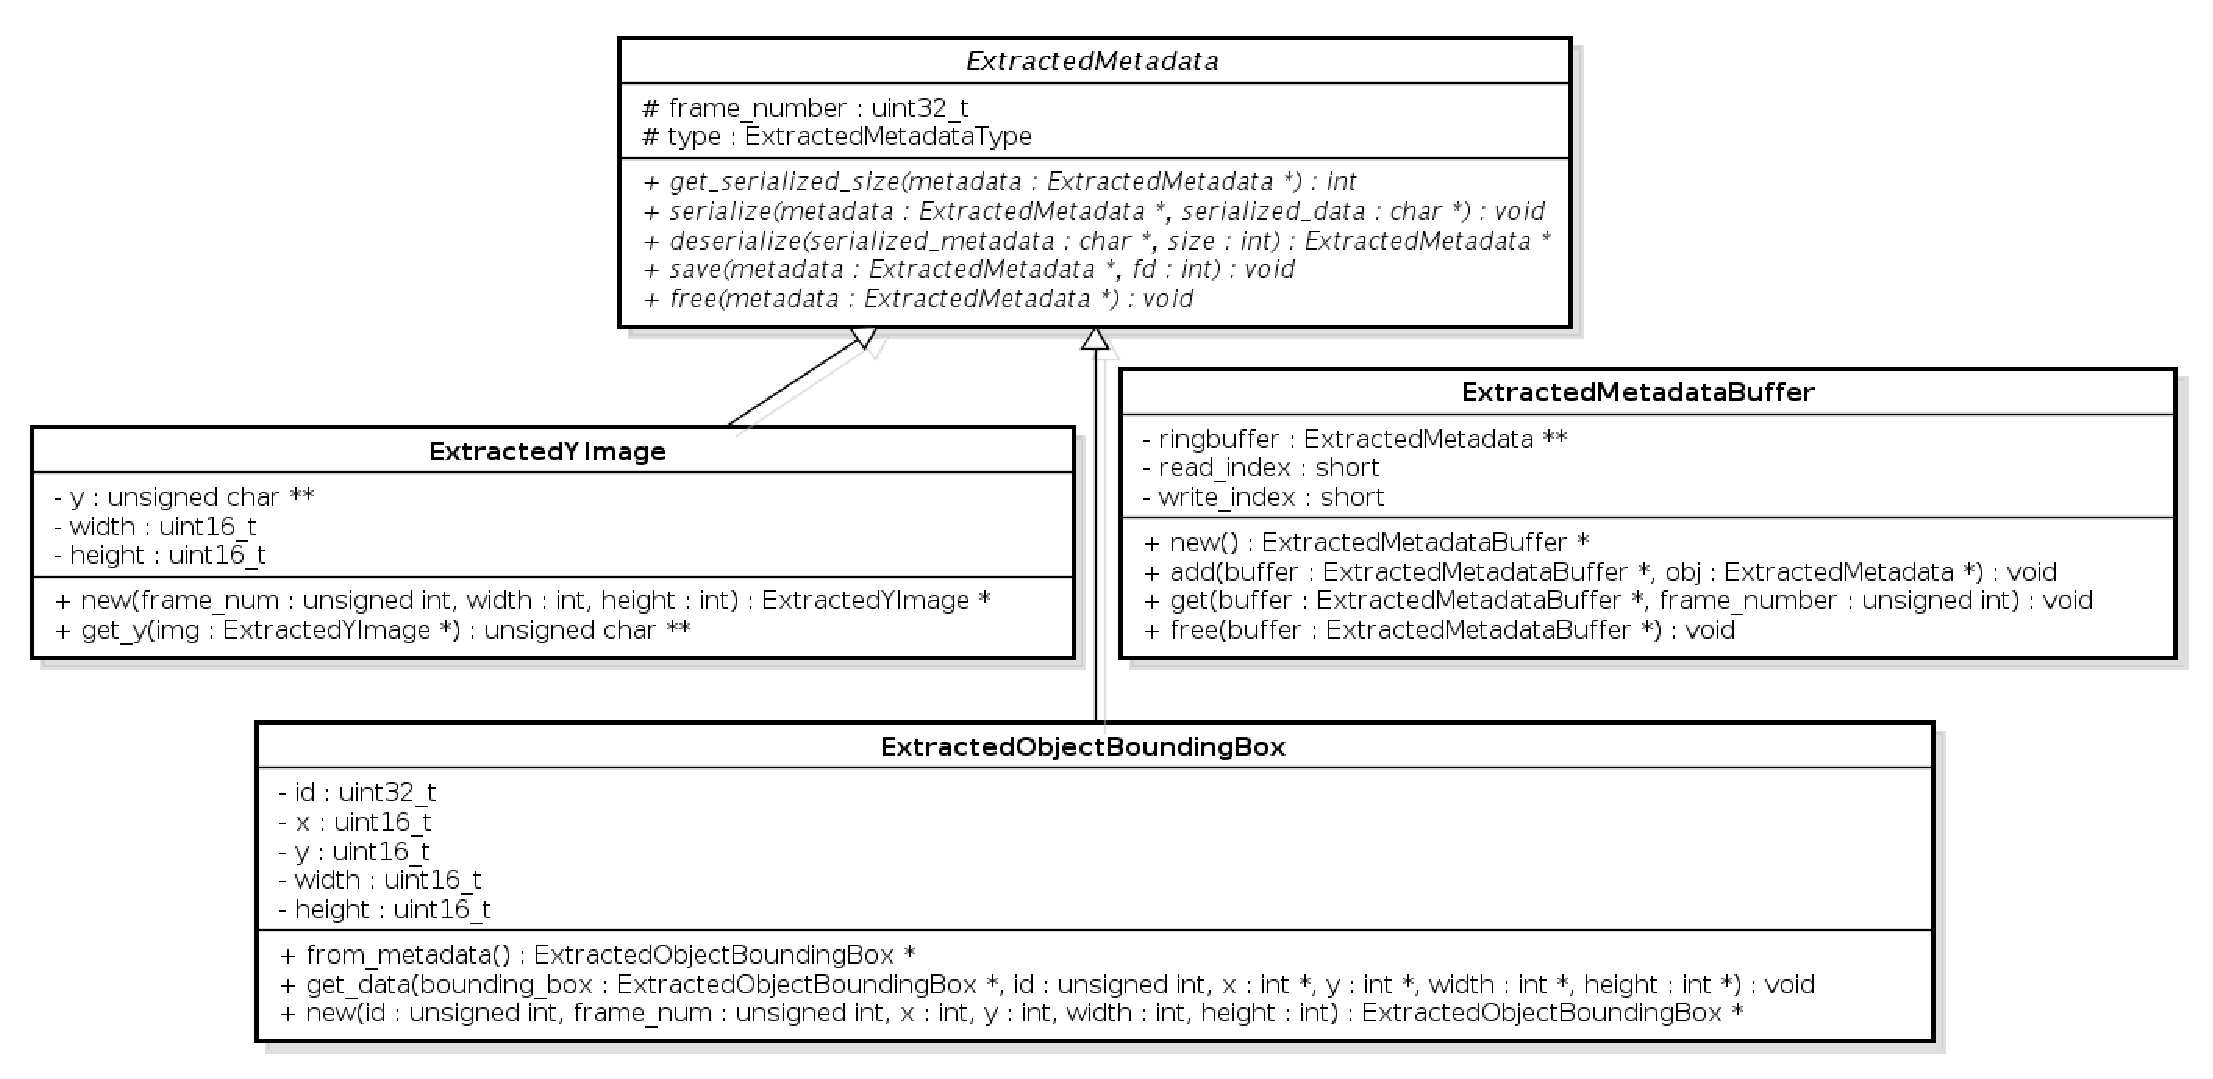
\includegraphics[scale=0.45]{imagens/fig10.eps}
\caption{Diagrama de classe dos objetos definidos no módulo extracted\_metadata.}
\label{fig:extracted_metadata_class_diagram}
\end{figure}

A implementação deste módulo encontra-se no apêndice B.


\subsection{ Extracted\_Metadata }

Esta classe abstrai a serialização, desserialização, salvamento e destruição dos diferentes tipos de metadados. O método \textit{serialize} é responsável pela serialização, que  é utilizada na inserção de um metadado no bitstream (utilizado em conjunto com o módulo \textit{udata\_gen}). 

O método \textit{get\_serialized\_size} é utilizado para auxiliar a alocação de memória necessária pelo processo de serialização, dessa maneira fica a cargo de quem está serializando o metadado alocar a memória necessária para a serialização e liberar a memória após o uso.

\begin{figure}[H]
\centering
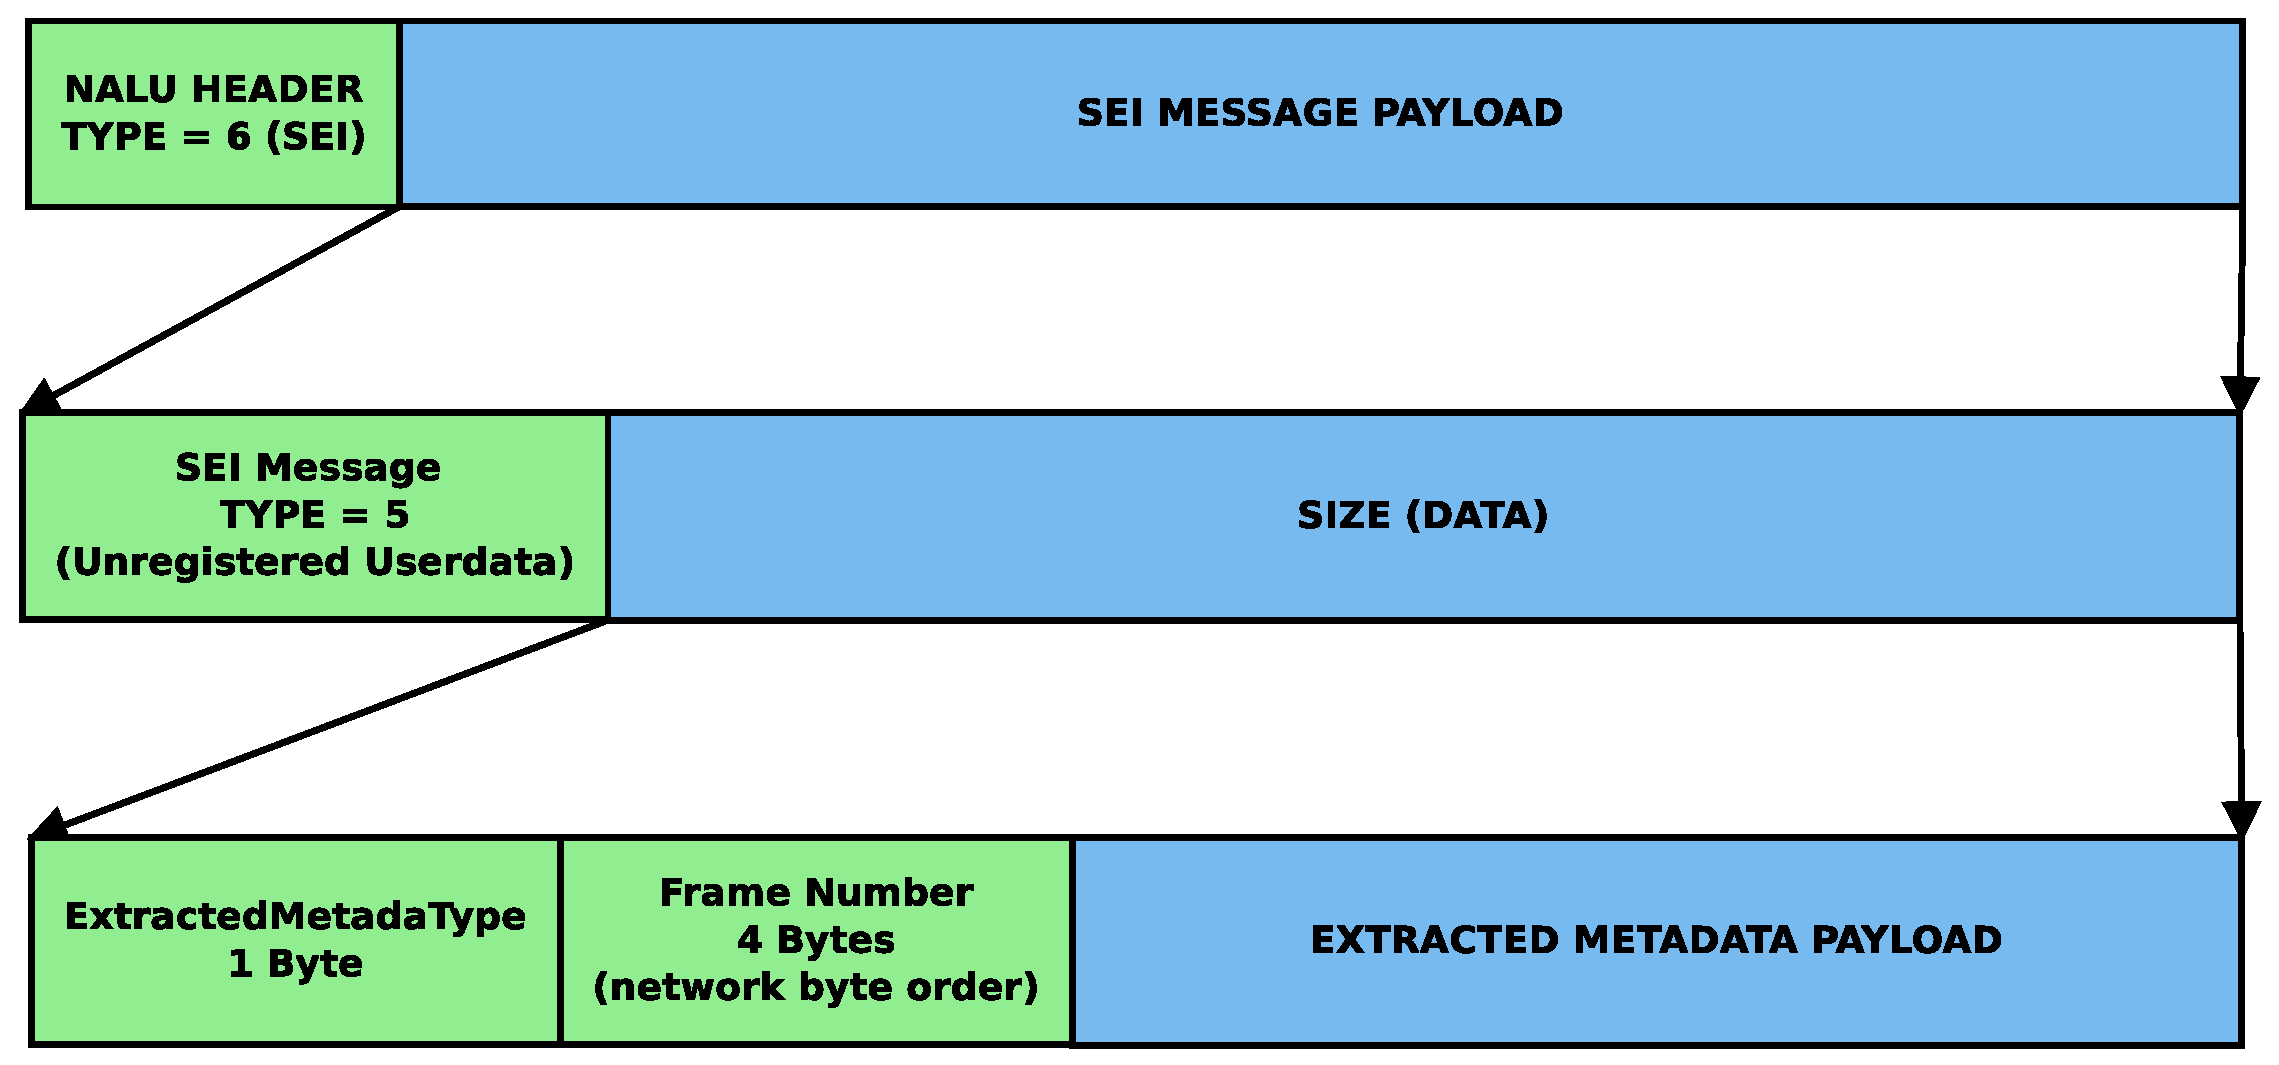
\includegraphics[scale=0.4]{imagens/fig9.eps}
\caption{Metadado serializado dentro de um NALU do tipo SEI. Cabeçalho em verde, \textit{payload} em azul.}
\label{fig:extracted_metadata_on_nalu}
\end{figure}

Como pode ser visto na figura ~\ref{fig:extracted_metadata_on_nalu}, um metadado serializado sempre começa com o seu tipo e o número do quadro (em ordem de apresentação) do qual ele foi extraído. O payload do metadado será definido pela classe que herdar \textit{ExtractedMetadata}.

O método \textit{save} salva o metadado em um file descriptor, sendo útil para realizar depuração. O método \textit{free} libera todos os recursos utilizados pelo metadado.


\subsection{ Extracted\_Y\_Image }


Esta classe herda \textit{ExtractedMetadata} e representa o plano luma de um objeto de interesse, é composto basicamente do plano luma com o seu comprimento e altura. O plano luma é um \textit{array} bidimensional de bytes, onde cada byte é o valor de um pixel. A primeira dimensão do array é a linha (Y) que vai de 0 á altura - 1. A segunda dimensão é a coluna (X), que vai de 0 á comprimento - 1.

Ao detectar um objeto de interesse é possível extrair apenas o objeto e inserir ele no bitstream. O objeto pode ser recuperado no decodificador e salvo em um arquivo. Como ele é composto apenas do plano luma só é possível visualizar o objeto monocromático. Muitos algoritmos trabalham com imagens monocromáticas, esse metadado pode ser utilizado para preservar no bitstream o objeto original antes que parte das informações dele possam ser destruídas pelo processo de codificação, dependendo do nível de perda do processo da codificação. 

Em alguns casos para economizar largura de banda na transmissão, ou espaço no armazenamento, o vídeo é obtido em alta definição mas tem seu tamanho reduzido, utilizando esse metadado seria possível dispor de um banco de objetos de interesse em alta resolução apesar dos vídeos terem seu tamanho reduzido.

Para criar um objeto \textit{ExtractedYImage} basta utilizar o método \textit{new} passando como parâmetro o número do quadro, seu comprimento e sua altura. Pela altura e comprimento informados será alocado o plano, que pode ser obtido através do método \textit{get\_y}, tendo obtido o plano basta escrever nele o plano luma do objeto e o metadado estará pronto para ser serializado e inserido no bitstream.


\begin{figure}[H]
\centering
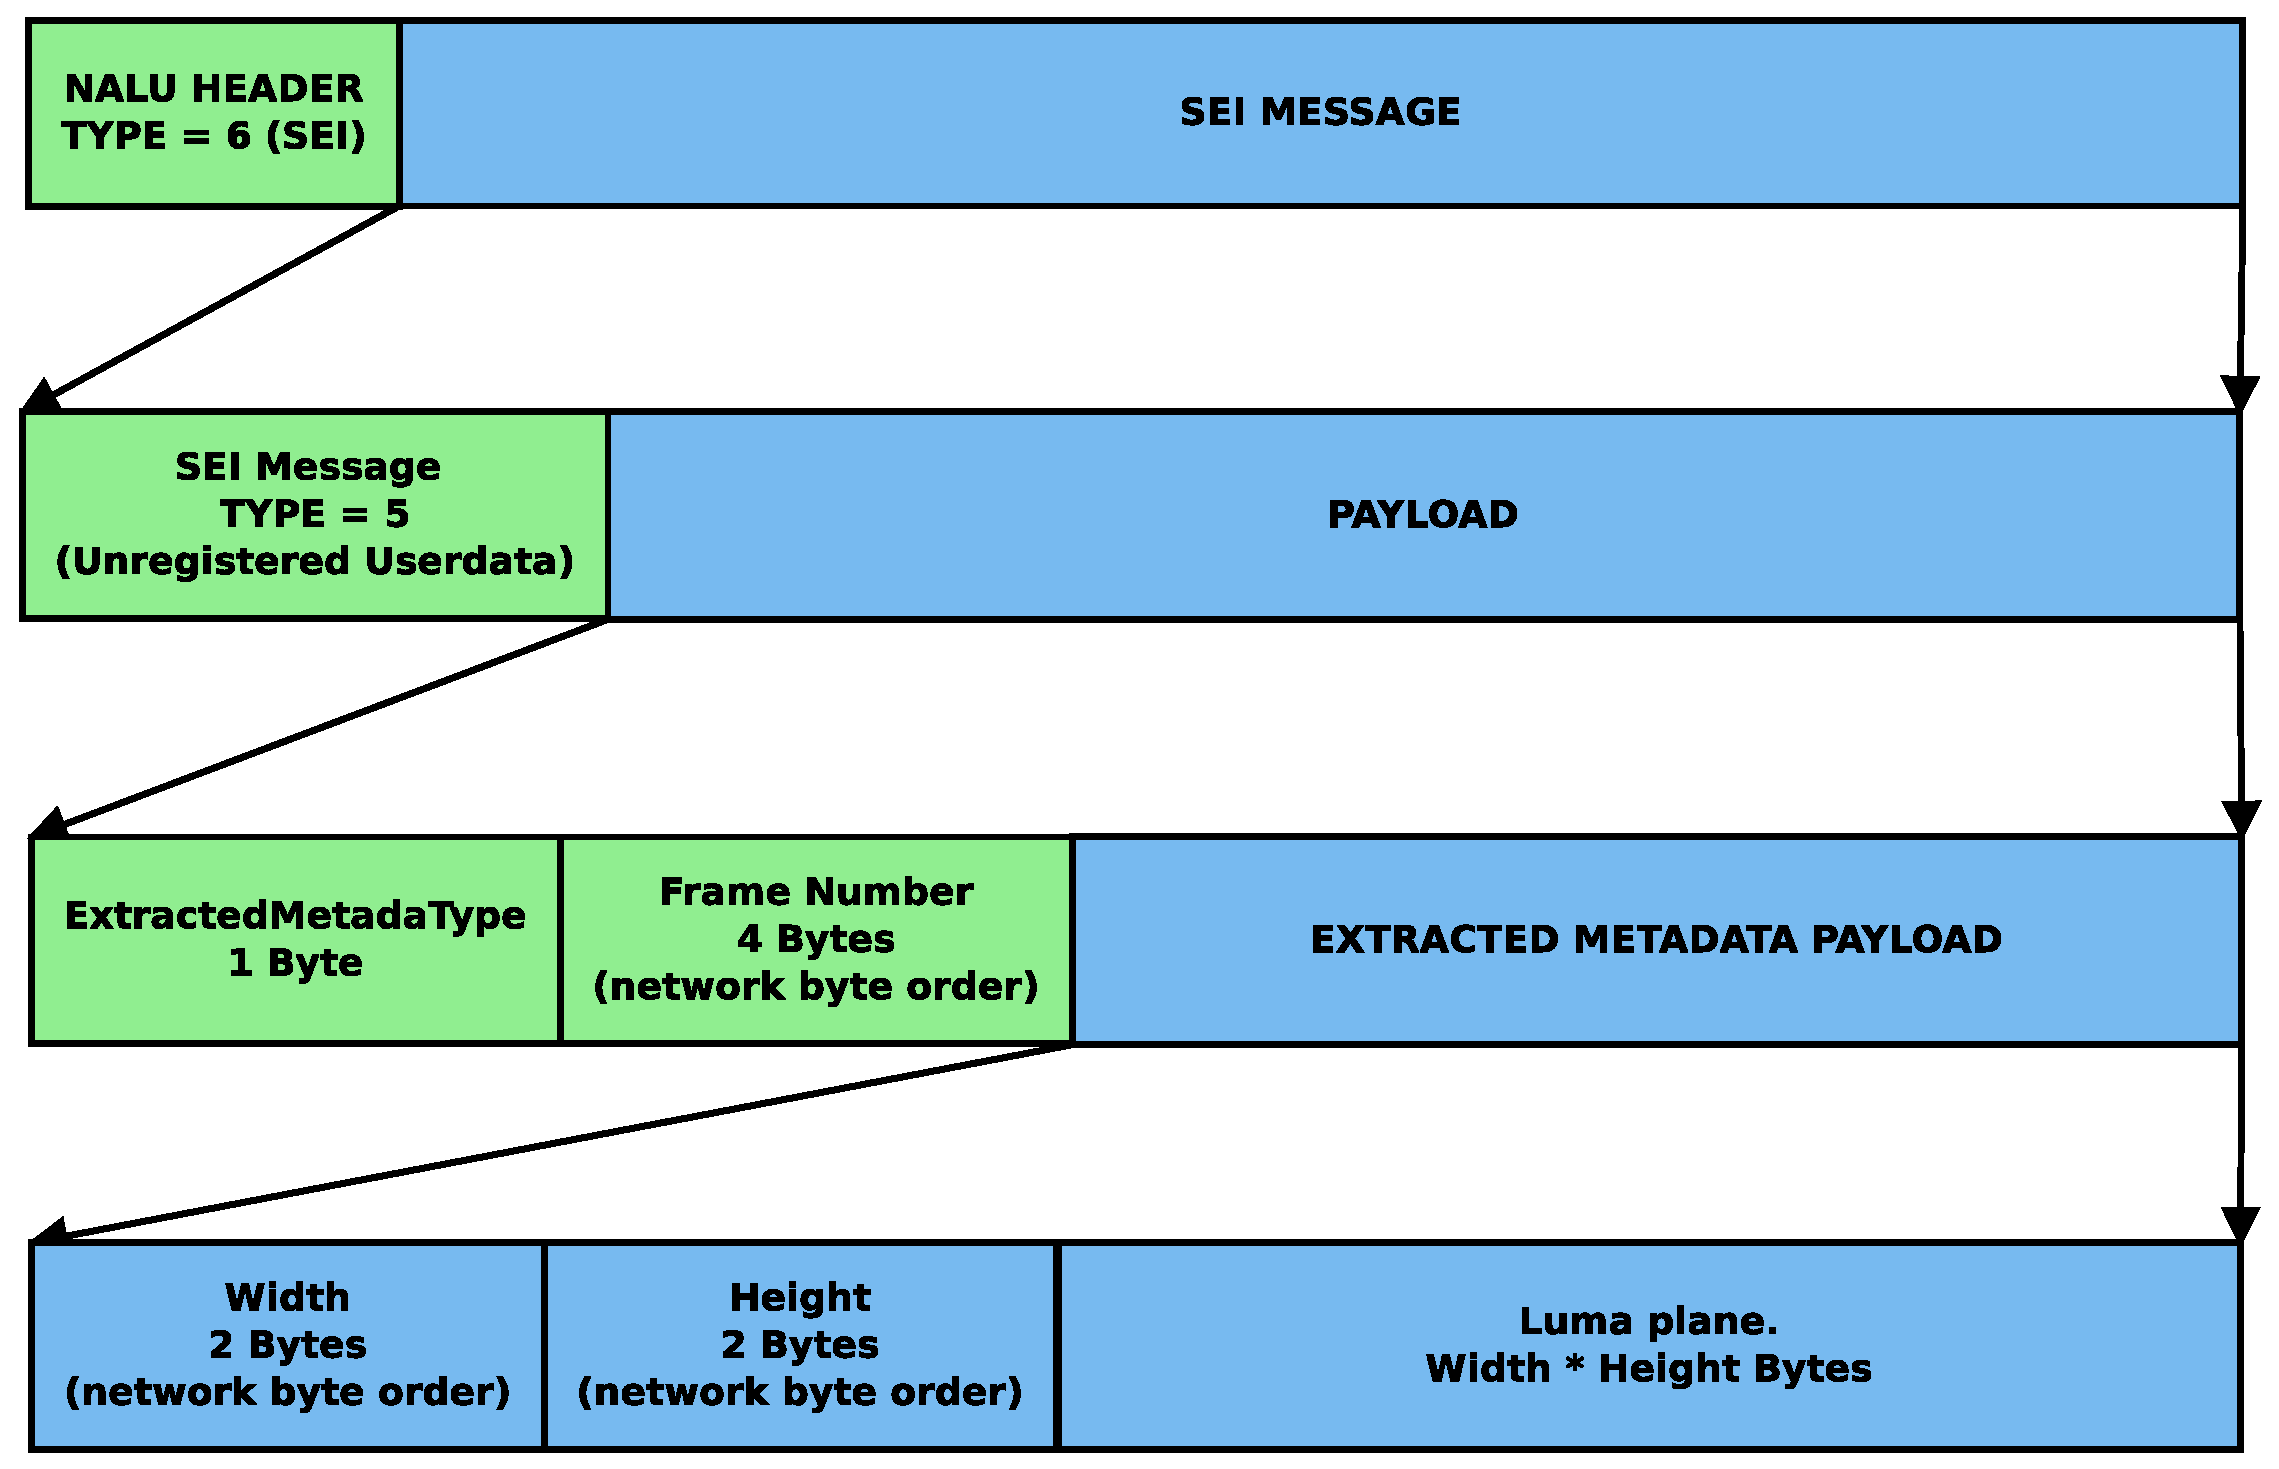
\includegraphics[scale=0.4]{imagens/fig11.eps}
\caption{Objeto ExtractedYImage serializado dentro de um NALU do tipo SEI. Cabeçalho em verde, \textit{payload} em azul.}
\label{fig:extracted_y_image_on_nalu}
\end{figure}


\subsection{ Extracted\_Object\_Bounding\_Box }


Esta classe herda \textit{ExtractedMetadata} e representa uma caixa delimitadora envolta de um objeto de interesse. Ela é composta de um identificador único do objeto, as coordenadas (x, y) da caixa, sua altura e seu comprimento.

Ao ocorrer a detecção de um objeto de interesse é possível inserir no bitstream um metadado \textit{ExtractedObjectBoundingBox}, ao ser recuperado no decodificador, utilizando o identificador único, é possível realizar a indexação de todos os objetos diferentes detectados ao longo do vídeo. Como a classe pai \textit{ExtractedMetadata} possui o número do quadro em ordem de apresentação, é possível dizer em que momento do vídeo o objeto foi detectado pela primeira vez e qual o momento que ele foi identificado pela última vez, tendo assim todo o intervalo de tempo em que o objeto esteve no vídeo.

Com as informações da caixa delimitadora também é possível desenhar a caixa diretamente no vídeo, facilitando a constatação visual de que um objeto de interesse está presente no trecho de vídeo. Se para cada quadro que possui o objeto de interesse for inserido um metadado \textit{ExtractedObjectBoundingBox} no bitstream será possível realizar o tracking do objeto ao longo do vídeo. 

Para criar um objeto \textit{ExtractedObjectBoundingBox} basta utilizar o método \textit{new} passando como parâmetro o identificador do objeto, o número do quadro (em ordem de apresentação), a coordenada x, a coordenada y, seu comprimento e sua altura. Após a construção basta serializar e inserir o objeto \textit{ExtractedObjectBoundingBox} no bitstream. 

Ao recuperar o metadado do bitstream o método \textit{get\_data} pode ser utilizado para se obter informações como o identificador único do objeto, suas coordenadas e seu tamanho.


\begin{figure}[H]
\centering
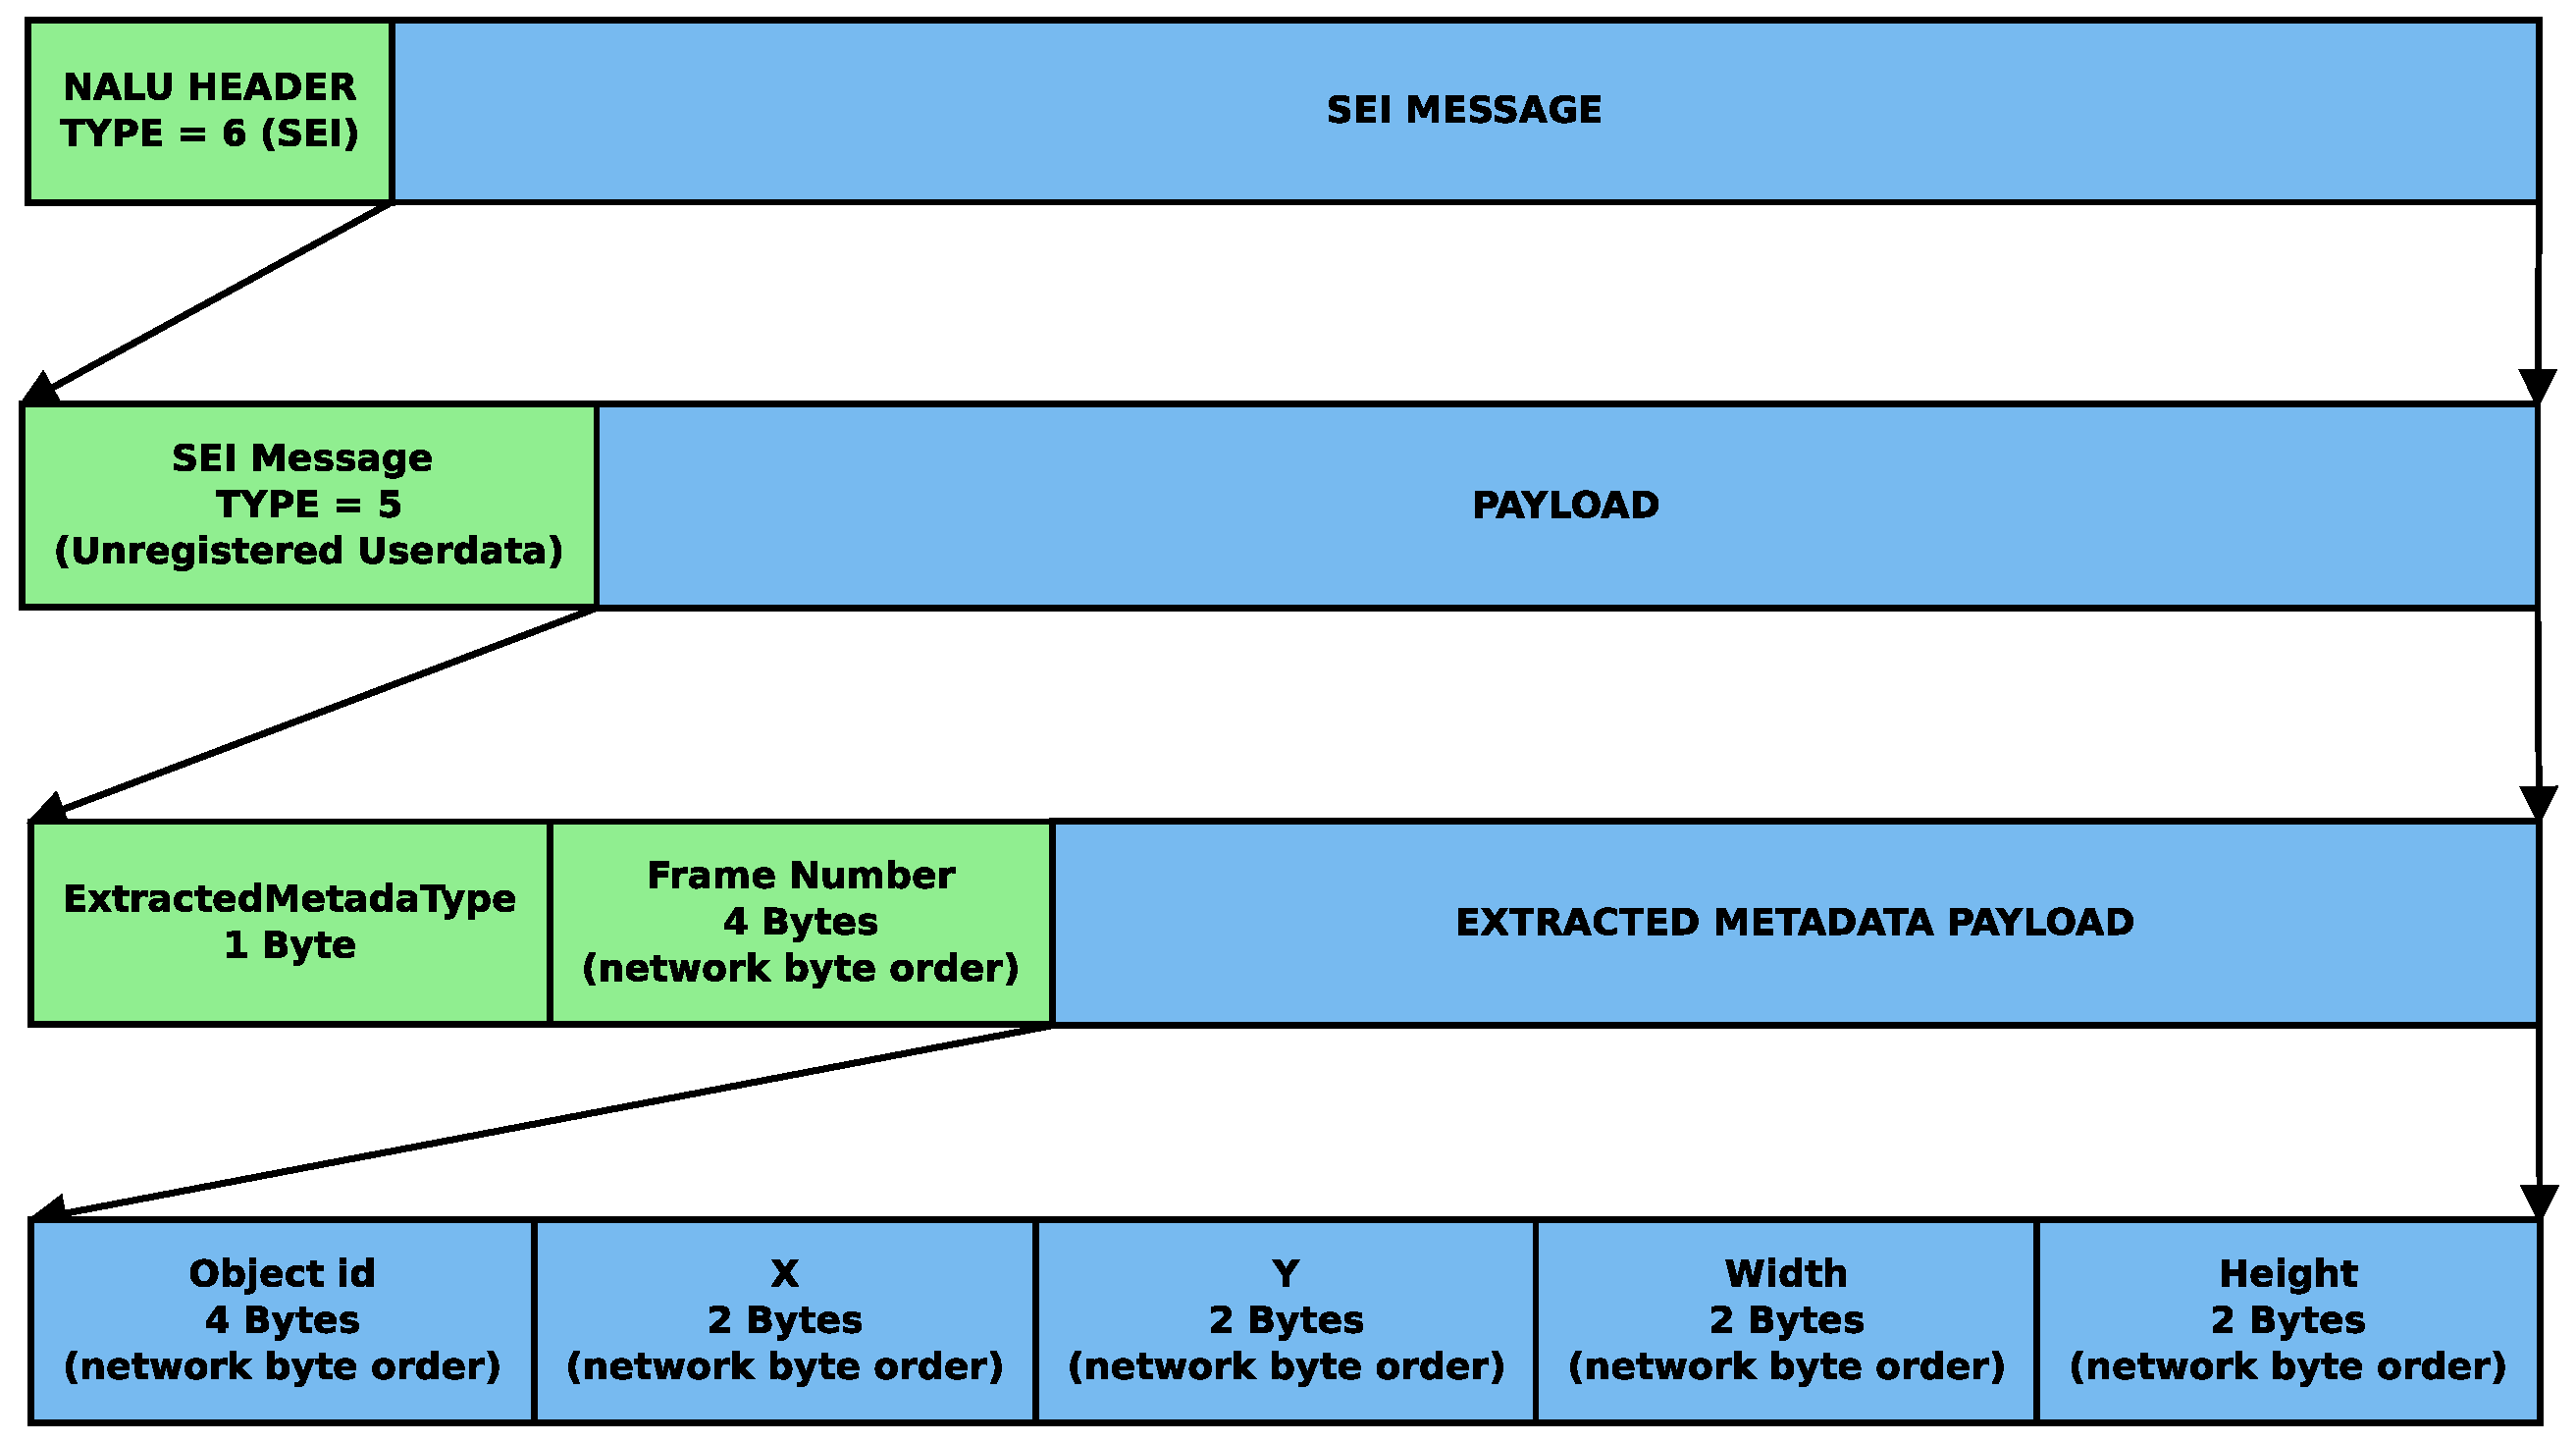
\includegraphics[scale=0.4]{imagens/fig12.eps}
\caption{Objeto ExtractedObjectBoundingBox serializado dentro de um NALU do tipo SEI. Cabeçalho em verde, \textit{payload} em azul.}
\label{fig:extracted_object_bounding_box_on_nalu}
\end{figure}


\subsection{ Extracted\_Metadata\_Buffer }

Esta classe é utilizada para bufferizar diversos metadados extraídos no processo de decodificação. O método \textit{add} adiciona um novo metadado no buffer, os metadados podem ser recuperados do buffer utilizando o método \textit{get}, neste método deve ser informado o número do quadro em ordem de apresentação, se houver algum metadado referente a este quadro ele será retornado, se não existir o método retornará \textit{NULL}.

O buffer foi construído porque nem sempre os metadados ficam no bitstream exatamente antes do quadro ao qual eles pertencem. Dependendo do vídeo vários metadados podem ser inseridos no bitstream antes que um quadro seja escrito no bitstream, dessa maneira é necessário bufferizar os metadados no decodificador até terminar a decodificação de um quadro e chegar o momento de apresentá-lo. Ao terminar a decodificação o buffer pode ser consultado para verificar se existe algum metadado referente ao quadro que será apresentado.

Para tornar a bufferização eficiente e simples não existe nenhum tipo de ordenação dos metadados dentro do buffer, ao se obter o metadado para um determinado quadro, qualquer metadado que for referente a um quadro anterior será descartado pelo buffer. Portanto um metadado deve ser gravado no bitstream antes do quadro do qual ele foi extraído. E os metadados devem sempre ser gravados no bitstream na ordem correta (os metadados referentes a quadros menores primeiro). Isso é fácil de garantir já que no codificador temos total controle de quando o metadado é gravado no bitstream, o que já não é verdade para os quadros que dependem de vários outros processos internos do codificador.

\begin{figure}[H]
\centering
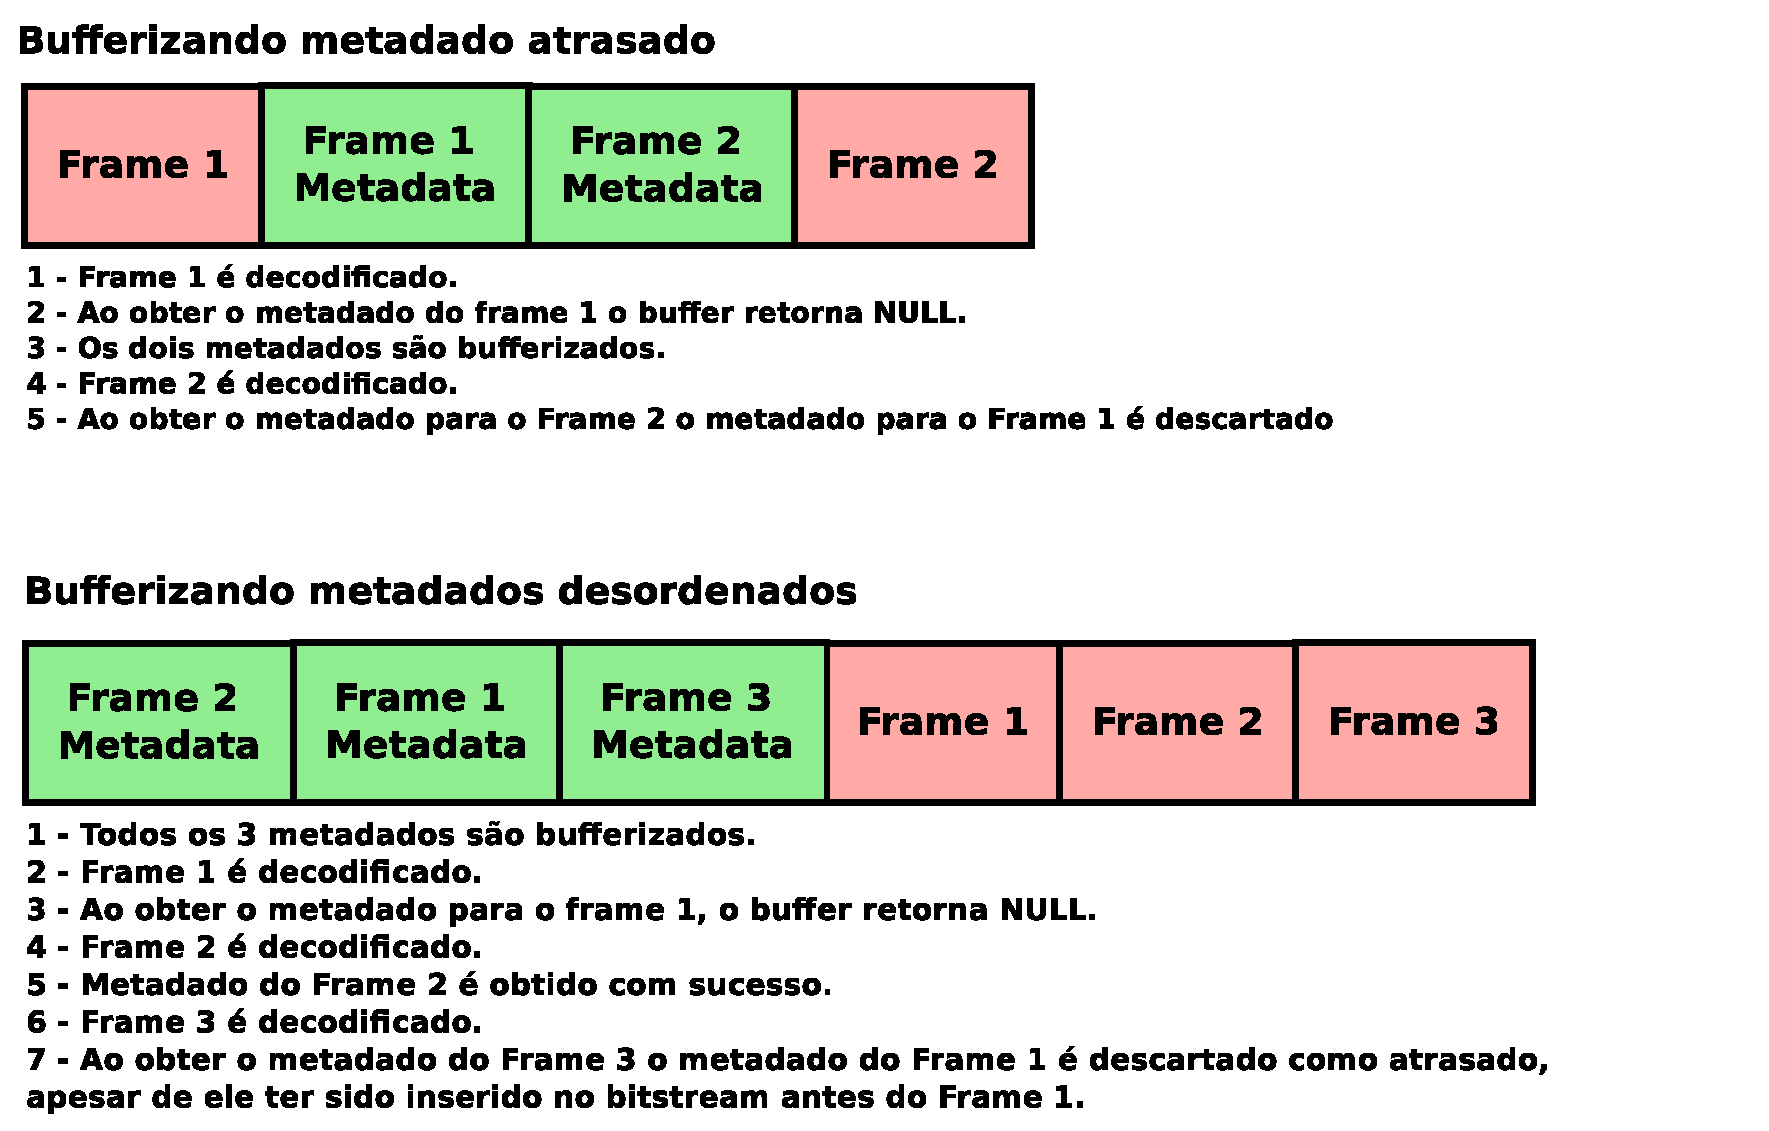
\includegraphics[scale=0.6]{imagens/fig13.eps}
\caption{Exemplo de problemas que podem ocorrer na recuperação dos metadados se eles forem inseridos de maneira errada no bitstream. Metadados em verde, quadros em vermelho.}
\label{fig:bad_metadada_ordering}
\end{figure}

A figura ~\ref{fig:bad_metadada_ordering} exemplifica alguns problemas que podem ocorrer ao bufferizar metadados que não foram inseridos no bitstream de maneira adequada.


\section{ Módulo metadata\_extractor }

Este módulo é responsável pela extração de metadados a partir de quadros brutos e das informações de estimativa de movimento fornecidas. Na atual implementação  ele pode extrair metadados do tipo \textit{ExtractedObjectBoundingBox} e \textit{ExtractedYImage}.

É escrito em linguagem C e se encontra no diretório \textit{lencod} do software de referência já que ele é utilizado tanto pelo codificador como pelo decodificador. Todas as funções são declaradas no cabeçalho \textit{lencod/inc/metadata\_extractor.h} e implementadas em \textit{lencod/src/metadata\_extractor.c}.

Nele também foi utilizada a mesma abordagem orientada a objetos utilizada no módulo \textit{extracted\_metadata} e as mesmas regras foram utilizadas para os nomes das funções que representam métodos da classe \textit{MetadataExtractor}.

O uso do classificador Haar na implementação do extrator de metadados será comentado nessa seção. A implementação completa do módulo encontra-se no apêndice C.


\subsection{ Metadata\_Extractor }

É o único objeto exportado publicamente pelo módulo e possui todo o contexto da extração de metadados. O método \textit{new} cria um novo extrator de metadados, na criação várias características do extrator podem ser configuradas por meio dos seguintes parâmetros: 

\begin{itemize}
	\item min\_width - Comprimento mínimo do objeto de interesse.
	\item min\_height - Altura mínima do objeto de interesse.
	\item search\_hysteresis - Histerese (em quadros) para realização da busca de um novo objeto de interesse.
	\item tracking\_hysteresis - Histerese (em quadros) para realizar a confirmação de que o objeto de interesse do qual está sendo feito \textit{tracking} ainda se encontra no vídeo, e corrigir possíveis erros causados pela estimativa de movimento.
        \item training\_file - Arquivo de treinamento que será utilizado ao criar o classificador Haar desse extrator. Ele define qual é o objeto de interesse.
\end{itemize}

O termo histerese tem diferentes significados de acordo com o contexto e a área em que é utilizado, pode ser utilizado na biologia, tratamento de materiais, mecânica, entre outros. No presente trabalho a histerese se refere a quantidade de quadros necessários para realizar a execução do classificador Haar, gerando um atraso configurável na detecção de um novo objeto, ou ao confirmar a existência de um objeto previamente detectado.

O método \textit{extract\_raw\_object} extrai do quadro o plano luma do objeto de interesse (se ele existir no quadro) e retorna como um objeto \textit{ExtractedMetadata}. Para realizar a extração é necessário passar os seguintes parâmetros:

\begin{itemize}
	\item extractor - Objeto \textit{MetadataExtractor}.
	\item frame\_number - Número do quadro (em ordem de apresentação) do qual será extraído o metadado.
	\item y - Plano luma, array bidimensional[y][x] de bytes, onde y vai de 0 á altura - 1 e x vai de 0 á comprimento - 1.
	\item width - Comprimento do quadro.
        \item height - Altura do quadro.
\end{itemize}

Se o objeto de interesse não se encontrar no quadro, esse método retorna \textit{NULL}. As configurações de histerese e as informações de estimativa de movimento não são utilizadas nesse método.

O método \textit{extract\_object\_bounding\_box} extrai do quadro uma caixa delimitadora que representa a área onde se encontra o objeto de interesse no quadro e retorna como um objeto \textit{ExtractedMetadata}. Para realizar a extração é necessário passar os seguintes parâmetros:

\begin{itemize}
	\item extractor - Objeto \textit{MetadataExtractor}.
	\item frame\_number - Número do quadro (em ordem de apresentação) do qual será extraído o metadado.
	\item y - Plano luma, array bidimensional[y][x] de bytes, onde y vai de 0 à altura - 1 e x vai de 0 ao comprimento - 1.
	\item width - Comprimento do quadro.
        \item height - Altura do quadro.
\end{itemize}

Se o objeto de interesse não se encontrar no quadro, esse método retorna \textit{NULL}. As configurações de histerese e as informações de estimativa de movimento são utilizadas nesse método de acordo com o estado interno do extrator. O comportamento do método depende do estado interno do extrator:

\begin{itemize}

	\item Não realizando \textit{tracking} - Será consultada a histerese de busca, se a histerese foi ultrapassada, o classificador Haar será utilizado para realizar a busca do objeto de interesse neste quadro. Se o objeto existir, o extrator cria um objeto \textit{TrackedBoundingBox} que será utilizado internamente para realizar o \textit{tracking} do objeto, passa para o estado \textit{Realizando tracking} e retorna um objeto \textit{ExtractedObjectBoundingBox}. Se o objeto não existir o extrator reinicia a histerese de busca, continua no estado atual e retorna \textit{NULL}. Se a histerese não foi ultrapassada o extrator continua no estado atual e retorna \textit{NULL}.

	\item Realizando \textit{tracking} - Será consultada a histerese de \textit{tracking}, se a histerese foi ultrapassada, o classificador Haar será utilizado para verificar se o objeto ainda se encontra no quadro atual, se o objeto não for encontrado o extrator volta ao estado \textit{Não realizando tracking} e retorna NULL. Se o objeto de interesse está no quadro o objeto \textit{TrackedBoundingBox} é atualizado de acordo com a posição encontrada pelo classificador Haar e um \textit{ExtractedObjectBoundingBox} é retornado. Se a histerese não foi ultrapassada será retornado um objeto \textit{ExtractedObjectBoundingBox} utilizando as informações de estimativa de movimento para calcular a posição atual do objeto \textit{TrackedBoundingBox}.

\end{itemize}


\begin{figure}[H]
\centering
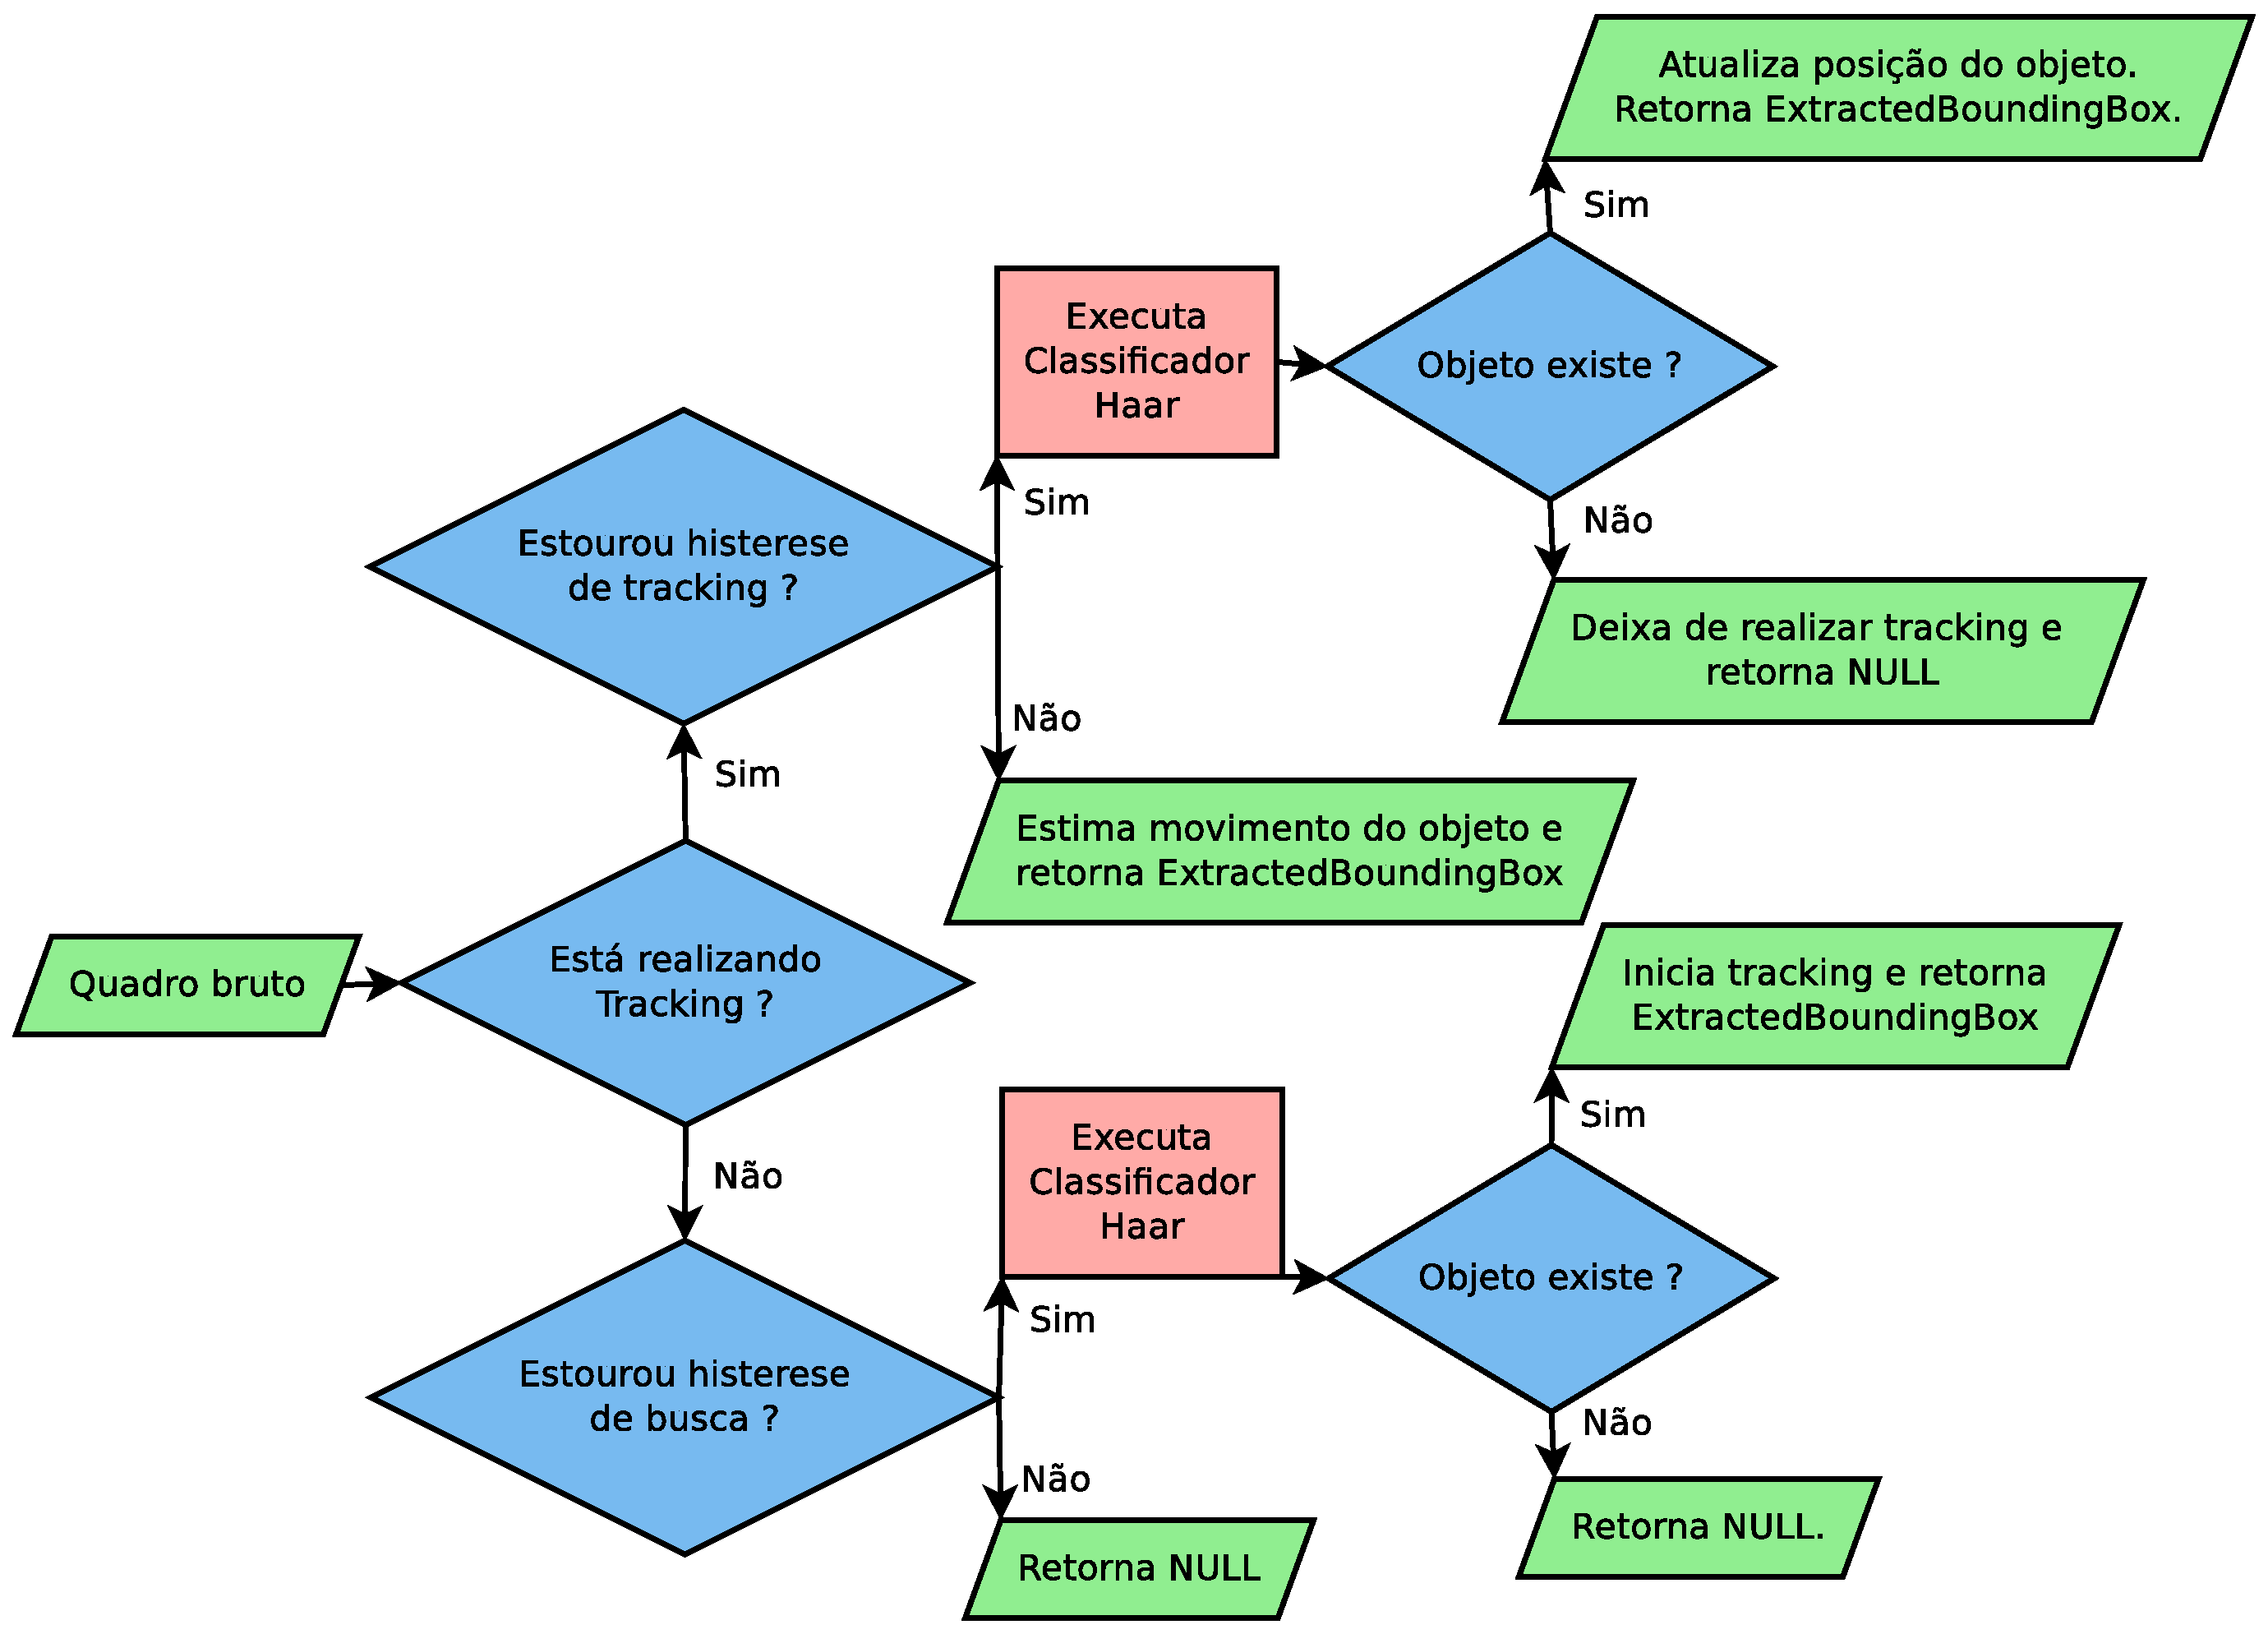
\includegraphics[scale=0.38]{imagens/fig14.eps}
\caption{Fluxograma do método extract\_object\_bounding\_box.}
\label{fig:extract_bounding_box_fluxogram}
\end{figure}

As histereses configuradas, junto com as informações de estimativa de movimento, visam utilizar os algoritmos já existentes no codificador para reduzir o custo computacional do \textit{tracking} de um objeto no vídeo. Ao invés de realizar o processamento de todos os quadros brutos no classificador Haar para realizar o \textit{tracking} do objeto ao longo do vídeo, a histerese diminui o custo computacional por atualizar a posição do objeto em intervalos fixos. Os vetores de movimento calculados pelo codificador são utilizados para suavizar o \textit{tracking}, estimando a nova posição do objeto enquanto a histerese de \textit{tracking} não estoura.

Por exemplo, em um vídeo com 300 quadros sem nenhum objeto de interesse, com uma histerese de busca de 10 quadros, o classificador Haar será chamado apenas 30 vezes, ao invés de 300 vezes. A configuração é especialmente útil em vídeos com \textit{framerate} muito alto, já que determinados objetos têm uma velocidade de locomoção esperada em um vídeo, logo não é necessário processar todos os quadros.

\begin{figure}[H]
\centering
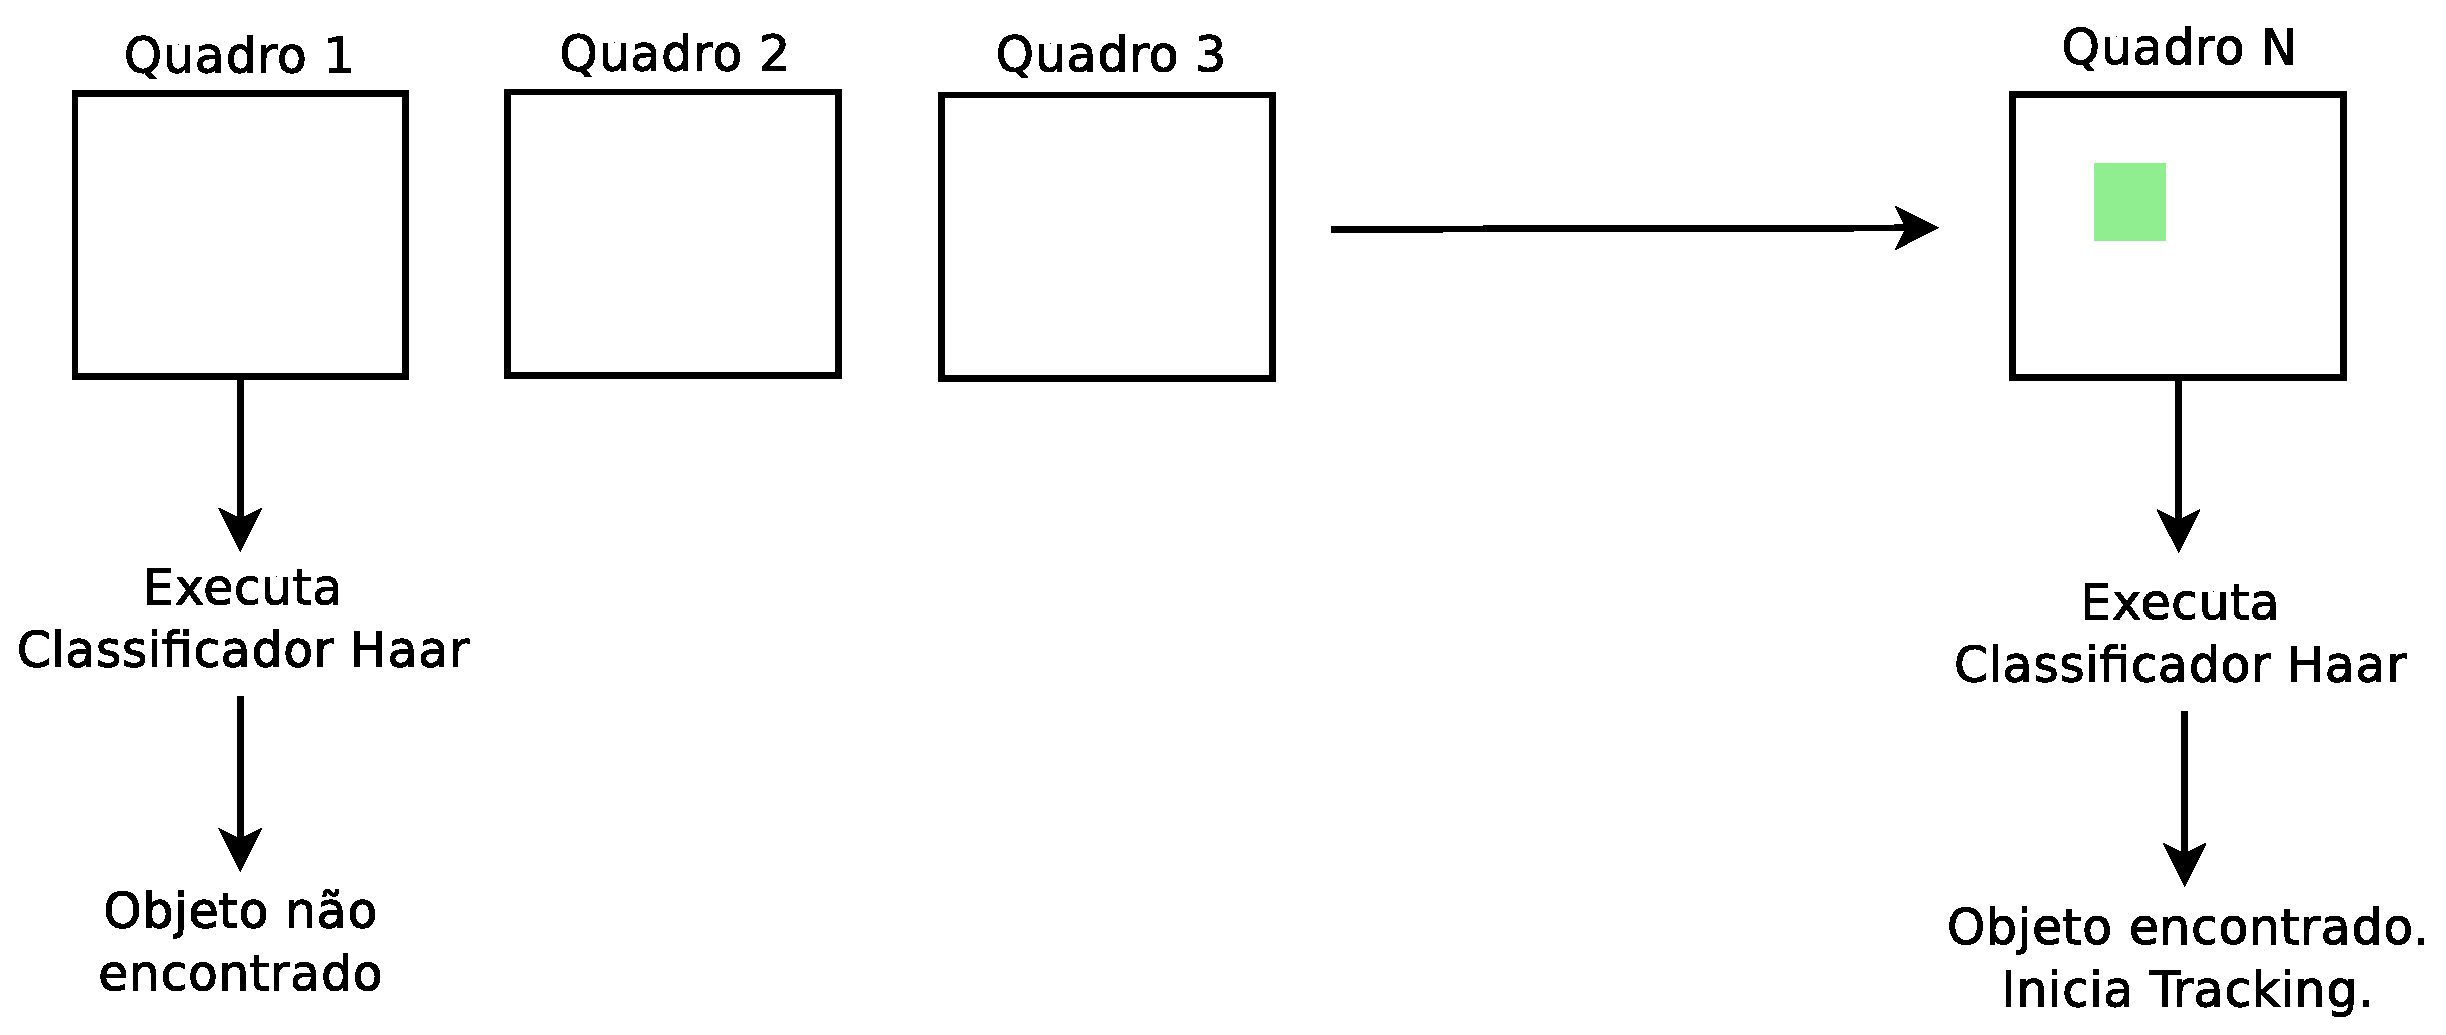
\includegraphics[scale=0.4]{imagens/fig23.eps}
\caption{Exemplo do funcionamento da histerese de busca.}
\label{fig:search_histeresys_example}
\end{figure}

O mesmo se dá quando o objeto já foi detectado, não é necessário executar o classificador em todos os quadros, os vetores de estimativa de movimento nos dão uma ideia aproximada da posição do objeto, até que seja alcançada a histerese de \textit{tracking}.

\begin{figure}[H]
\centering
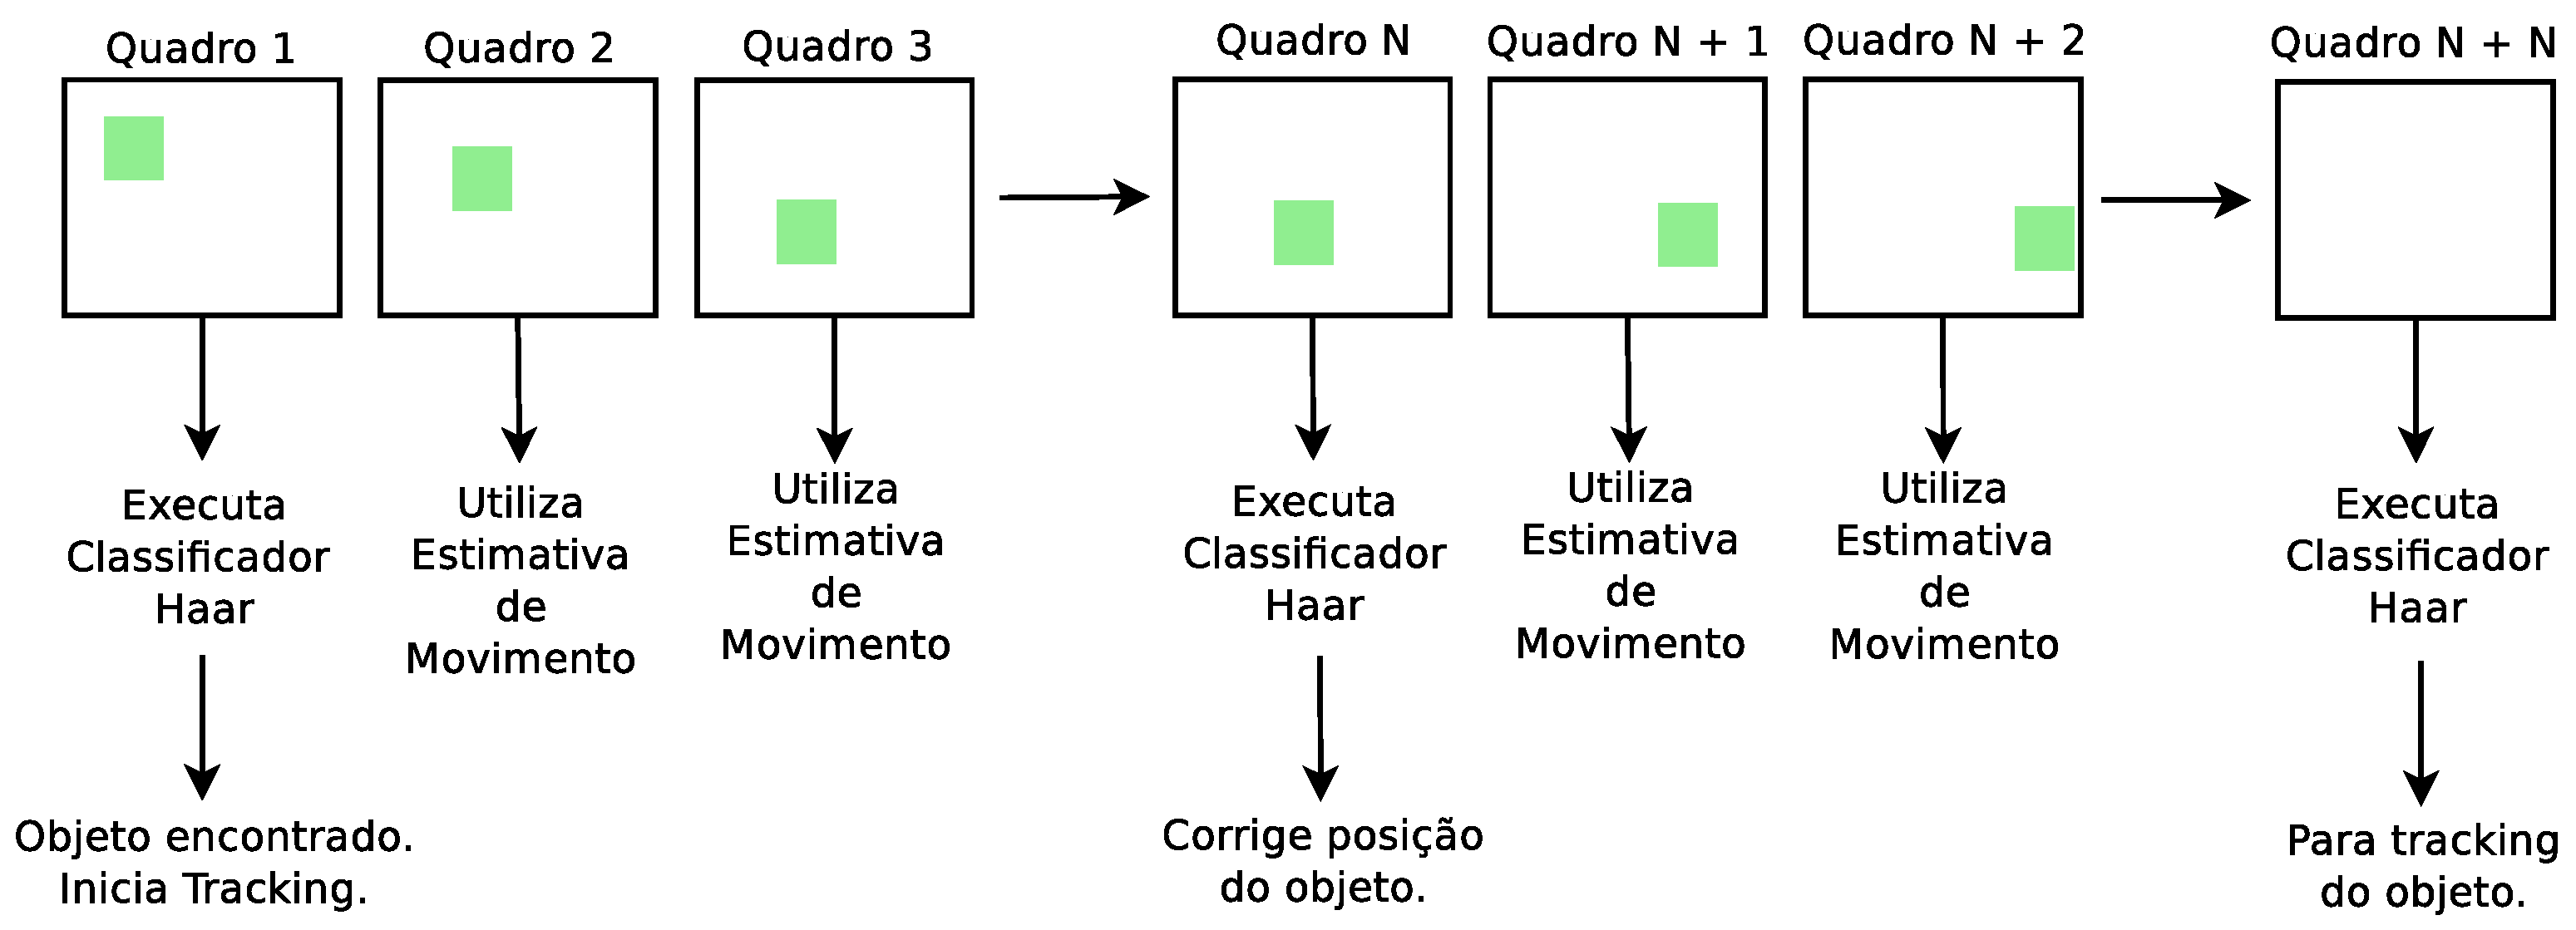
\includegraphics[scale=0.3]{imagens/fig24.eps}
\caption{Exemplo do funcionamento da histerese de \textit{tracking}.}
\label{fig:tracking_histeresys_example}
\end{figure}

Cada extrator só pode realizar a monitoração de um objeto de interesse, se existirem diversos objetos de interesse no quadro ele irá detectar apenas um e realizar o \textit{tracking} desse objeto. Criar vários extratores para detectar o mesmo tipo de objeto geraria problemas como detectar várias vezes o mesmo objeto, mas seria possível criar vários extratores para detectar objetos diferentes e utilizá-los em paralelo.


\subsection{ Utilizando o classificador Haar }


O classificador Haar foi escolhido como algoritmo de detecção de padrões a ser utilizado nesse trabalho. Como ele ficou completamente oculto na implementação do módulo \textit{metadata\_extractor} é possível alterar a implementação do módulo, utilizando outro algoritmo de detecção de padrões, sem realizar qualquer alteração na API pública do módulo, ou simplesmente removê-lo. A única limitação da API atual é que ela trabalha apenas com as informações de luminância, para trabalhar com algoritmos que utilizem informações de cor será necessária uma alteração na API do módulo atual.

A implementação do classificador Haar do OpenCV foi escolhida para realizar a detecção de objetos por ser bem documentada e fácil de utilizar, sem contar que o OpenCV já dispõe de uma série de outras funções que facilitam trabalhar com o quadro bruto. Outra vantagem é que ele trabalha com imagens em escala de cinza, independente da configuração do vídeo bruto o plano de luminância sempre possui a maior resolução possível. Técnicas que utilizam informações de cor teriam a desvantagem de ter de trabalhar com informações de cor com resolução reduzida. 

Outra motivação é a possibilidade de acelerar o classificador Haar diretamente em hardware, como pode ser visto em  \cite{haarFPGA}, onde a parte mais complexa do classificador Haar (90\% do tempo de processamento) foi implementando em hardware, o que se alinha com a ideia de construir um chip codificador H.264 com detecção de objetos integrada em tempo real. 

A principal função que é utilizada na detecção de um objeto é \textit{cvHaarDetectObjects( const CvArr* image, CvHaarClassifierCascade* cascade, CvMemStorage* storage, double scale\_factor, int min\_neighbors, int flags, CvSize min\_size)}.

O primeiro parâmetro é a imagem onde será realizada a busca, em escala de cinza, que será obtida através do plano luma original do codificador. O segundo parâmetro é o classificador que é criado no método \textit{new} do objeto \textit{MetadataExtractor}. O terceiro parâmetro é o buffer de trabalho do classificador que também é criado no método \textit{new}. 

O classificador busca pelo objeto de interesse em todas as escalas possíveis, o quarto parâmetro significa o quão grande será o pulo entre cada escala, um valor alto vai tornar o classificador mais rápido porém aumentará as chances de falso negativo. O quinto parâmetro é um controle para prevenir falsos positivos. Na área onde se encontra o objeto de interesse costuma ocorrer várias detecções com sucesso para o mesmo objeto, já que os pixels ao redor da área e em escalas diferentes indicam que existe o objeto de interesse. Por exemplo, o valor 3 indica que o classificador só considerará o objeto como presente se ocorrerem 3 detecções sobrepostas na mesma área.

O sexto parâmetro são as flags do processo de busca, existem 4 flags que podem ser compostas com o operador OR:

\begin{itemize}
	\item CV\_HAAR\_DO\_CANNY\_PRUNING - Fará com que regiões planas da imagem (sem linhas) sejam ignoradas.    
	\item CV\_HAAR\_SCALE\_IMAGE - Faz com que o classificador escalone a imagem em vez de escalonar ele mesmo.
	\item CV\_HAAR\_FIND\_BIGGEST\_OBJECT - Faz com que o classificador retorne apenas o maior objeto detectado (se houver mais de um).
	\item CV\_HAAR\_DO\_ROUGH\_SEARCH - Só pode ser utilizado em conjunto com a flag CV\_HAAR\_FIND\_BIGGEST\_OBJECT, faz com que o classificador encerre a busca assim que ele encontrar o objeto de interesse (nesse caso o maior).
\end{itemize}

O sétimo parâmetro é o tamanho mínimo que o objeto deve possuir para ser detectado pelo classificador. Quanto maior for o tamanho mínimo mais rápido o classificador irá executar, mas maior será a possibilidade de ocorrer falso negativo.


\subsection{ Realizando estimativa de movimento }

A estimativa de movimento de um objeto é realizada por um trabalho em conjunto entre o método \textit{extract\_object\_bounding\_box} e o método \textit{add\_motion\_estimation\_info}. Um \textit{MetadataExtractor} recebe as informações de estimativa de movimento através do método \textit{add\_motion\_estimation\_info}, essas informações por sua vez serão utilizadas na execução do método \textit{extract\_object\_bounding\_box}. O método \textit{add\_motion\_estimation\_info} recebe os seguintes parâmetros:

\begin{itemize}
	\item extractor - Objeto \textit{MetadataExtractor}.
        \item block\_x - X do bloco, em coordenada de bloco.
        \item block\_y - Y do bloco, em coordenada de bloco.
        \item x\_motion\_estimation - Estimativa de movimento para a coordenada x do bloco.
        \item y\_motion\_estimation - Estimativa de movimento para a coordenada y do bloco.
\end{itemize}

Se o extrator não estiver realizando \textit{tracking} de um objeto a chamada para este método é ignorada. Se o extrator está realizando \textit{tracking}, será avaliado se este bloco faz parte da caixa delimitadora (representada pela classe \textit{TrackedBoundingBox}) do objeto de interesse. Se qualquer parte do bloco estiver dentro da caixa delimitadora, as informações de estimativa de movimento dele serão utilizadas para estimar o movimento da caixa delimitadora do objeto de interesse.

Essa abordagem é eficiente já que bastam algumas comparações bem simples para verificar se a área do bloco tem uma interseção com a área da caixa delimitadora do objeto de interesse, porém a caixa delimitadora nem sempre representa perfeitamente o objeto (o objeto teria de ter a forma de uma caixa também), dessa maneira acaba-se utilizando a estimativa de movimento de blocos que fazem parte da caixa delimitadora mas não do objeto, gerando um erro que se acumula a cada estimativa de movimento do objeto. Isso limita o uso da técnica, sendo necessária uma histerese de \textit{tracking} pequena dependendo do quanto o objeto se movimenta e da sua caixa delimitadora.

No software de referência utiliza-se um modelo simplificado de estimativa de movimento, o tamanho dos blocos utilizados na estimativa de movimento sempre possuem um tamanho de 4 x 4 pixels, independente do modo escolhido. Dessa maneira para obter as coordenadas reais do bloco basta multiplicar as coordenadas do bloco por 4. Tendo as coordenadas reais do bloco fica fácil determinar se o bloco está dentro ou não da caixa delimitadora do objeto de interesse.


\begin{figure}[H]
\centering
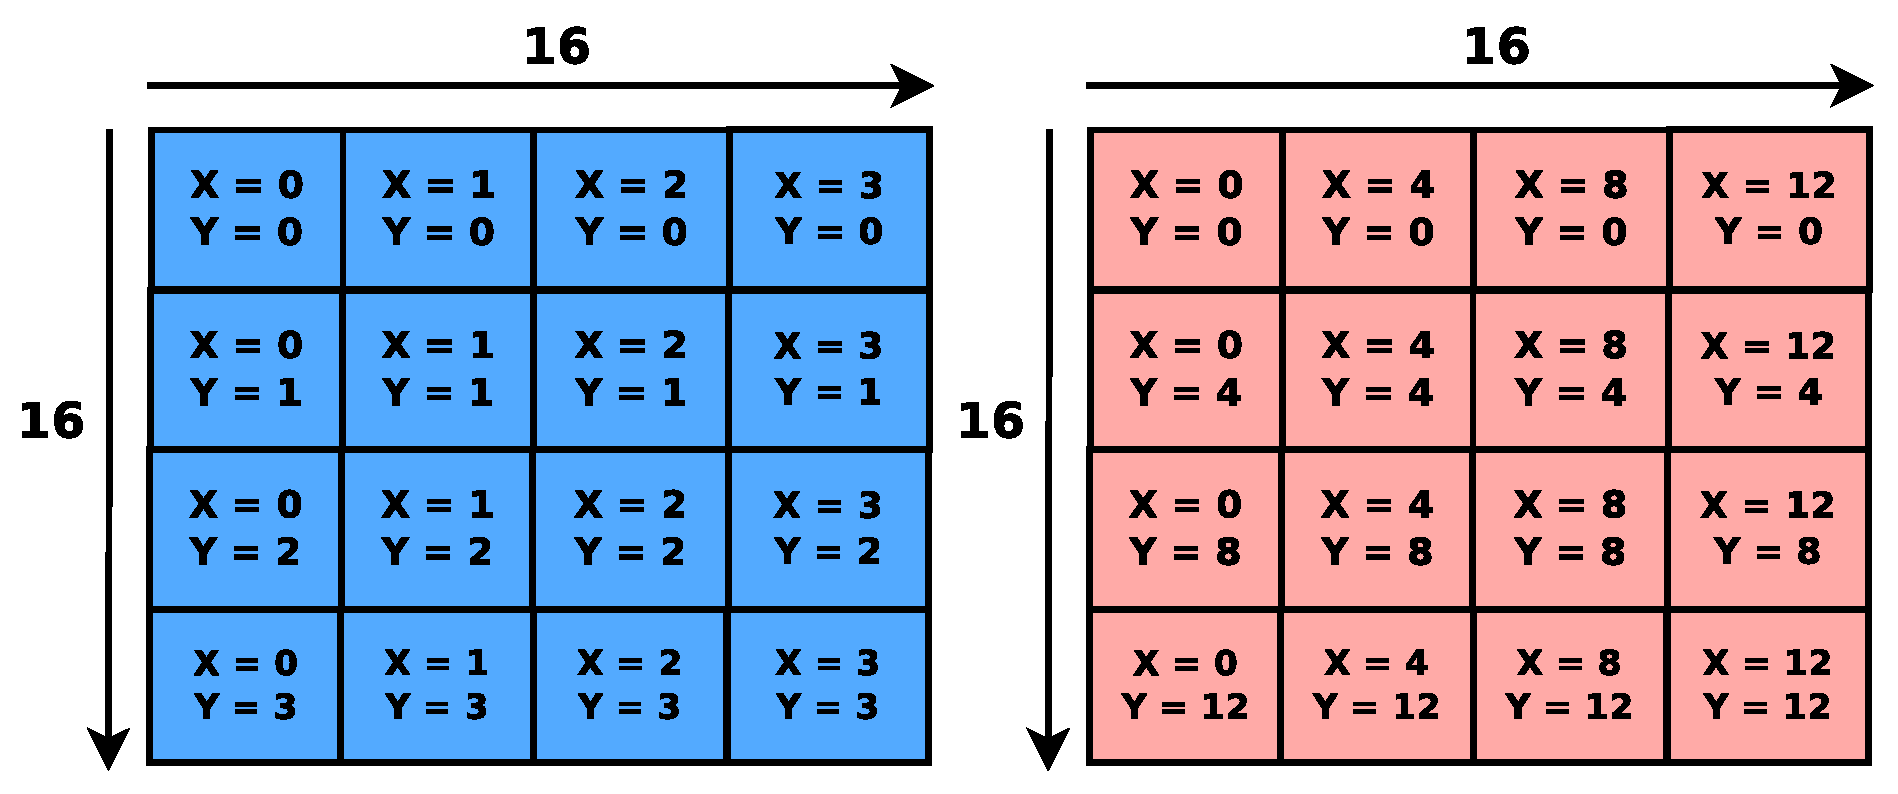
\includegraphics[scale=0.4]{imagens/fig16.eps}
\caption{Comparação entre as coordenadas dos blocos (em azul) da estimativa de movimento e as coordenadas reais (em vermelho) que elas representam.}
\label{fig:block_coordinate_example}
\end{figure}


É importante ressaltar que o tamanho fixo 4 x 4 para os blocos da estimativa de movimento não é verdade para todos os codificadores. Alguns codificadores possuem uma hierarquia e seria necessário derivar a estimativa de movimento para um bloco dependendo do modo utilizado.

O valor da estimativa de movimento é informado em unidades de QPel (Quarter Pel refinement), onde um quarto das amostras são sub-amostras interpoladas, causadas por frações de vetores de movimento.  Mais detalhes a respeito desse processo podem ser encontrados em \cite{ituh264avc} subcláusula 8.4.2.2. Um vetor x negativo indica um movimento para a direita, y negativo indica um movimento para baixo, x positivo indica um movimento para a esquerda e um y positivo um movimento para cima.


\begin{figure}[H]
\centering
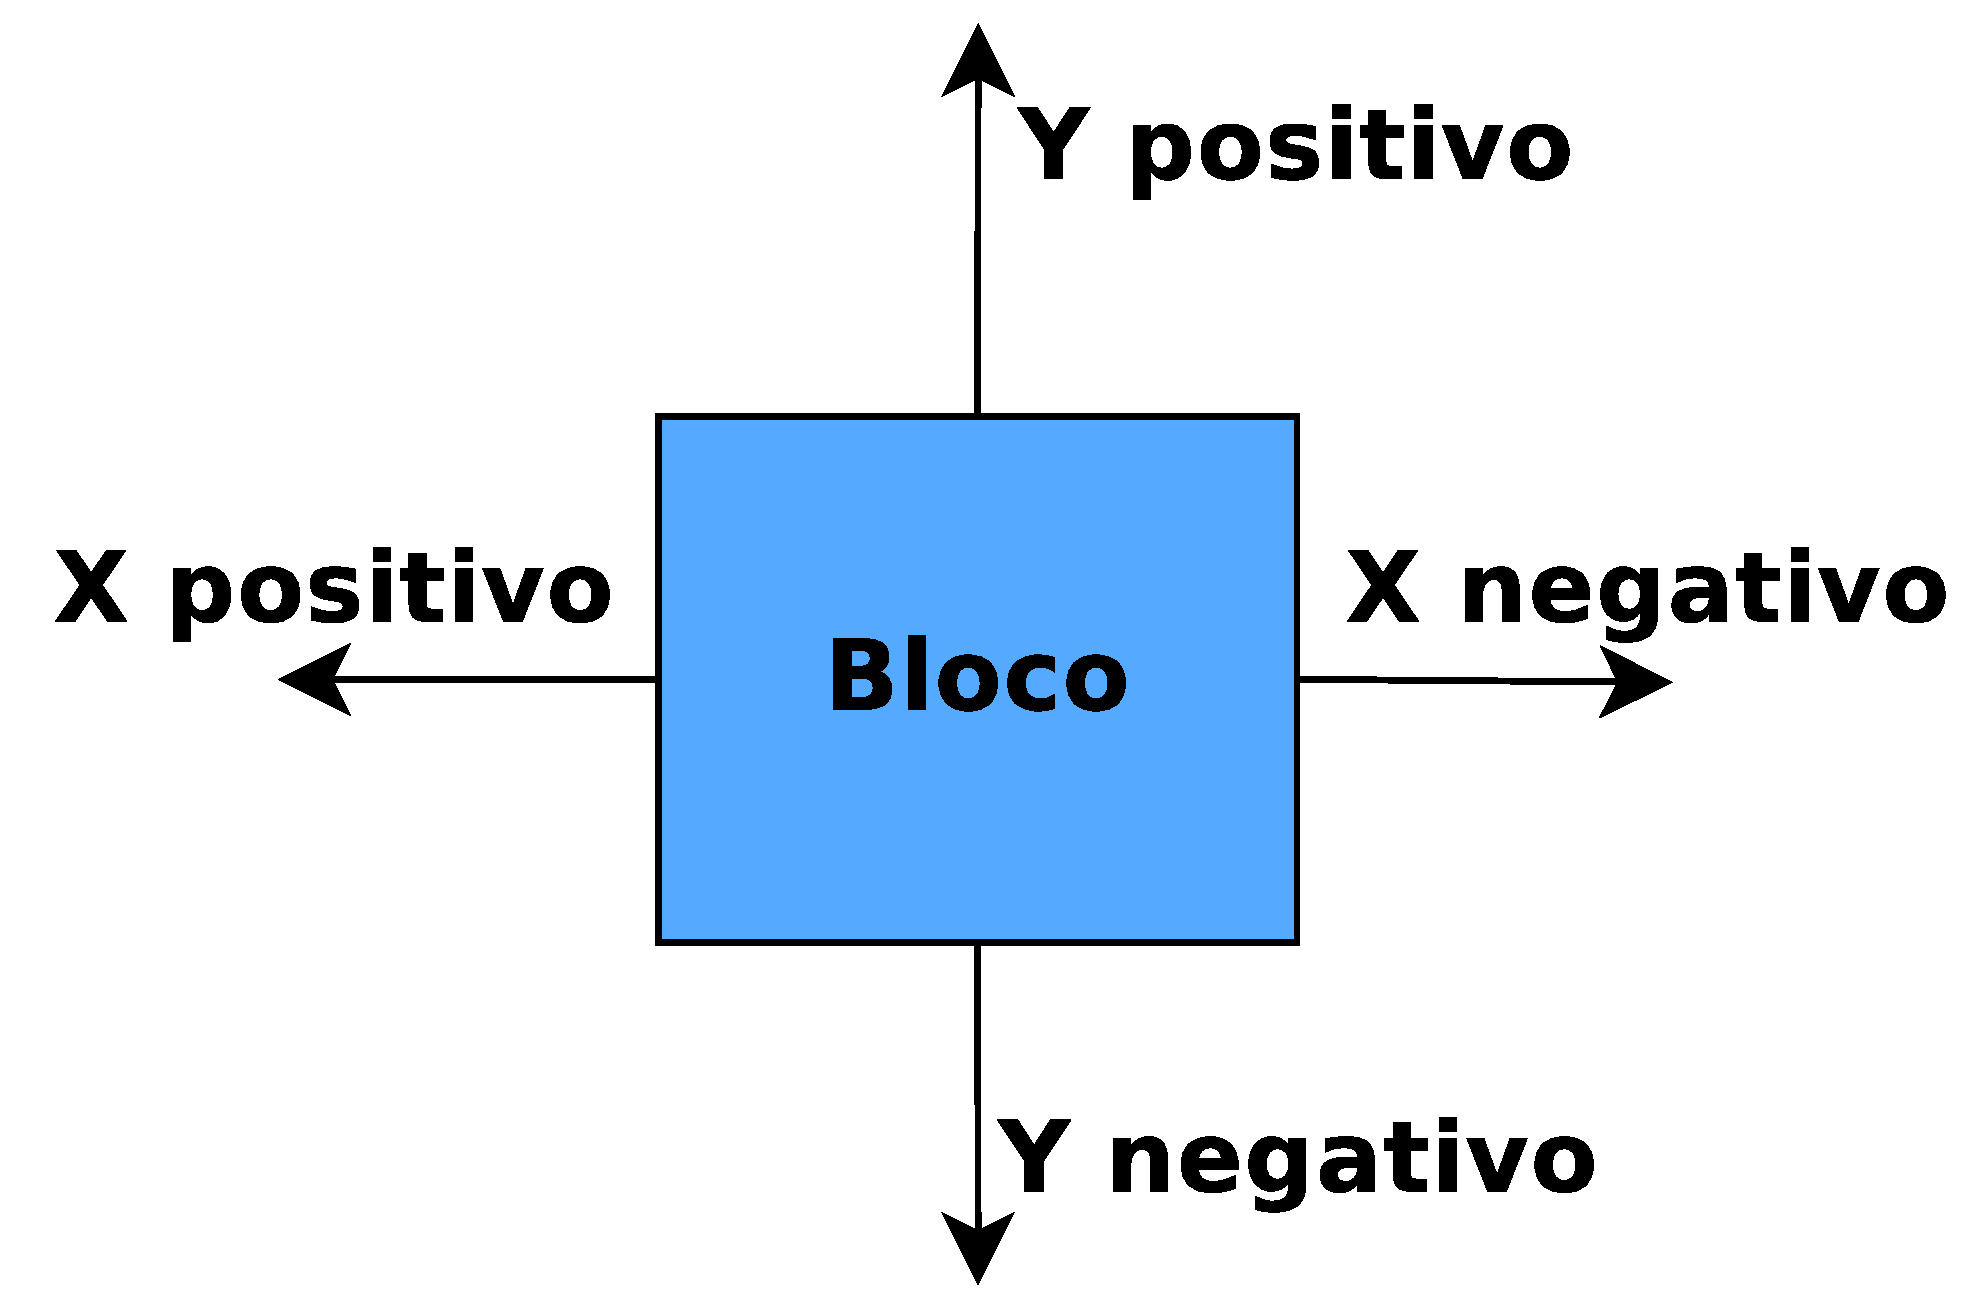
\includegraphics[scale=0.3]{imagens/fig15.eps}
\caption{Como os vetores de movimento de um bloco representam a sua movimentação no vídeo.}
\label{fig:block_vector_example}
\end{figure}


Todas as informações relativas a estimativa de movimento do objeto de interesse são guardadas no \textit{TrackedBoundingBox}, essa classe representa a caixa delimitadora do objeto de interesse do qual está sendo feito o \textit{tracking}, e é criada quando se identifica um objeto de interesse pela primeira vez. Nele é guardado um somatório de todos os vetores (em QPel) de movimento alimentados no extrator. Ao chamar o método \textit{extract\_object\_bounding\_box} no estado de \textit{tracking}, serão utilizadas as informações contidas no \textit{TrackedBoundingBox} para realizar a estimativa de movimento do objeto.

Nesse método é realizada a média aritmética simples de todos os vetores, ou seja o somatório de todos os vetores é dividido pela quantidade de blocos que foram utilizados para realizar a estimativa de movimento. O somatório de todos os vetores é dividido por 4 antes de ser dividido pela quantidade de blocos, pois o somatório dos vetores está em unidades de QPel. Realizar essa divisão por 4 nos fornece a estimativa de movimento em pixels. 

Tendo a estimativa de movimento em pixels basta subtrair a estimativa das coordenadas da \textit{TrackedBoundingBox}. Essas novas coordenadas serão utilizadas para criar o \textit{ExtractedObjectBoundingBox} que é retornado. As coordenadas (x,y) são guardadas como double no \textit{TrackedBoundingBox} para que não ocorra perda de precisão no acúmulo de pequenos movimentos, como pode ser visto na figura ~\ref{fig:object_motion_estimation_example}. 


\begin{figure}[H]
\centering
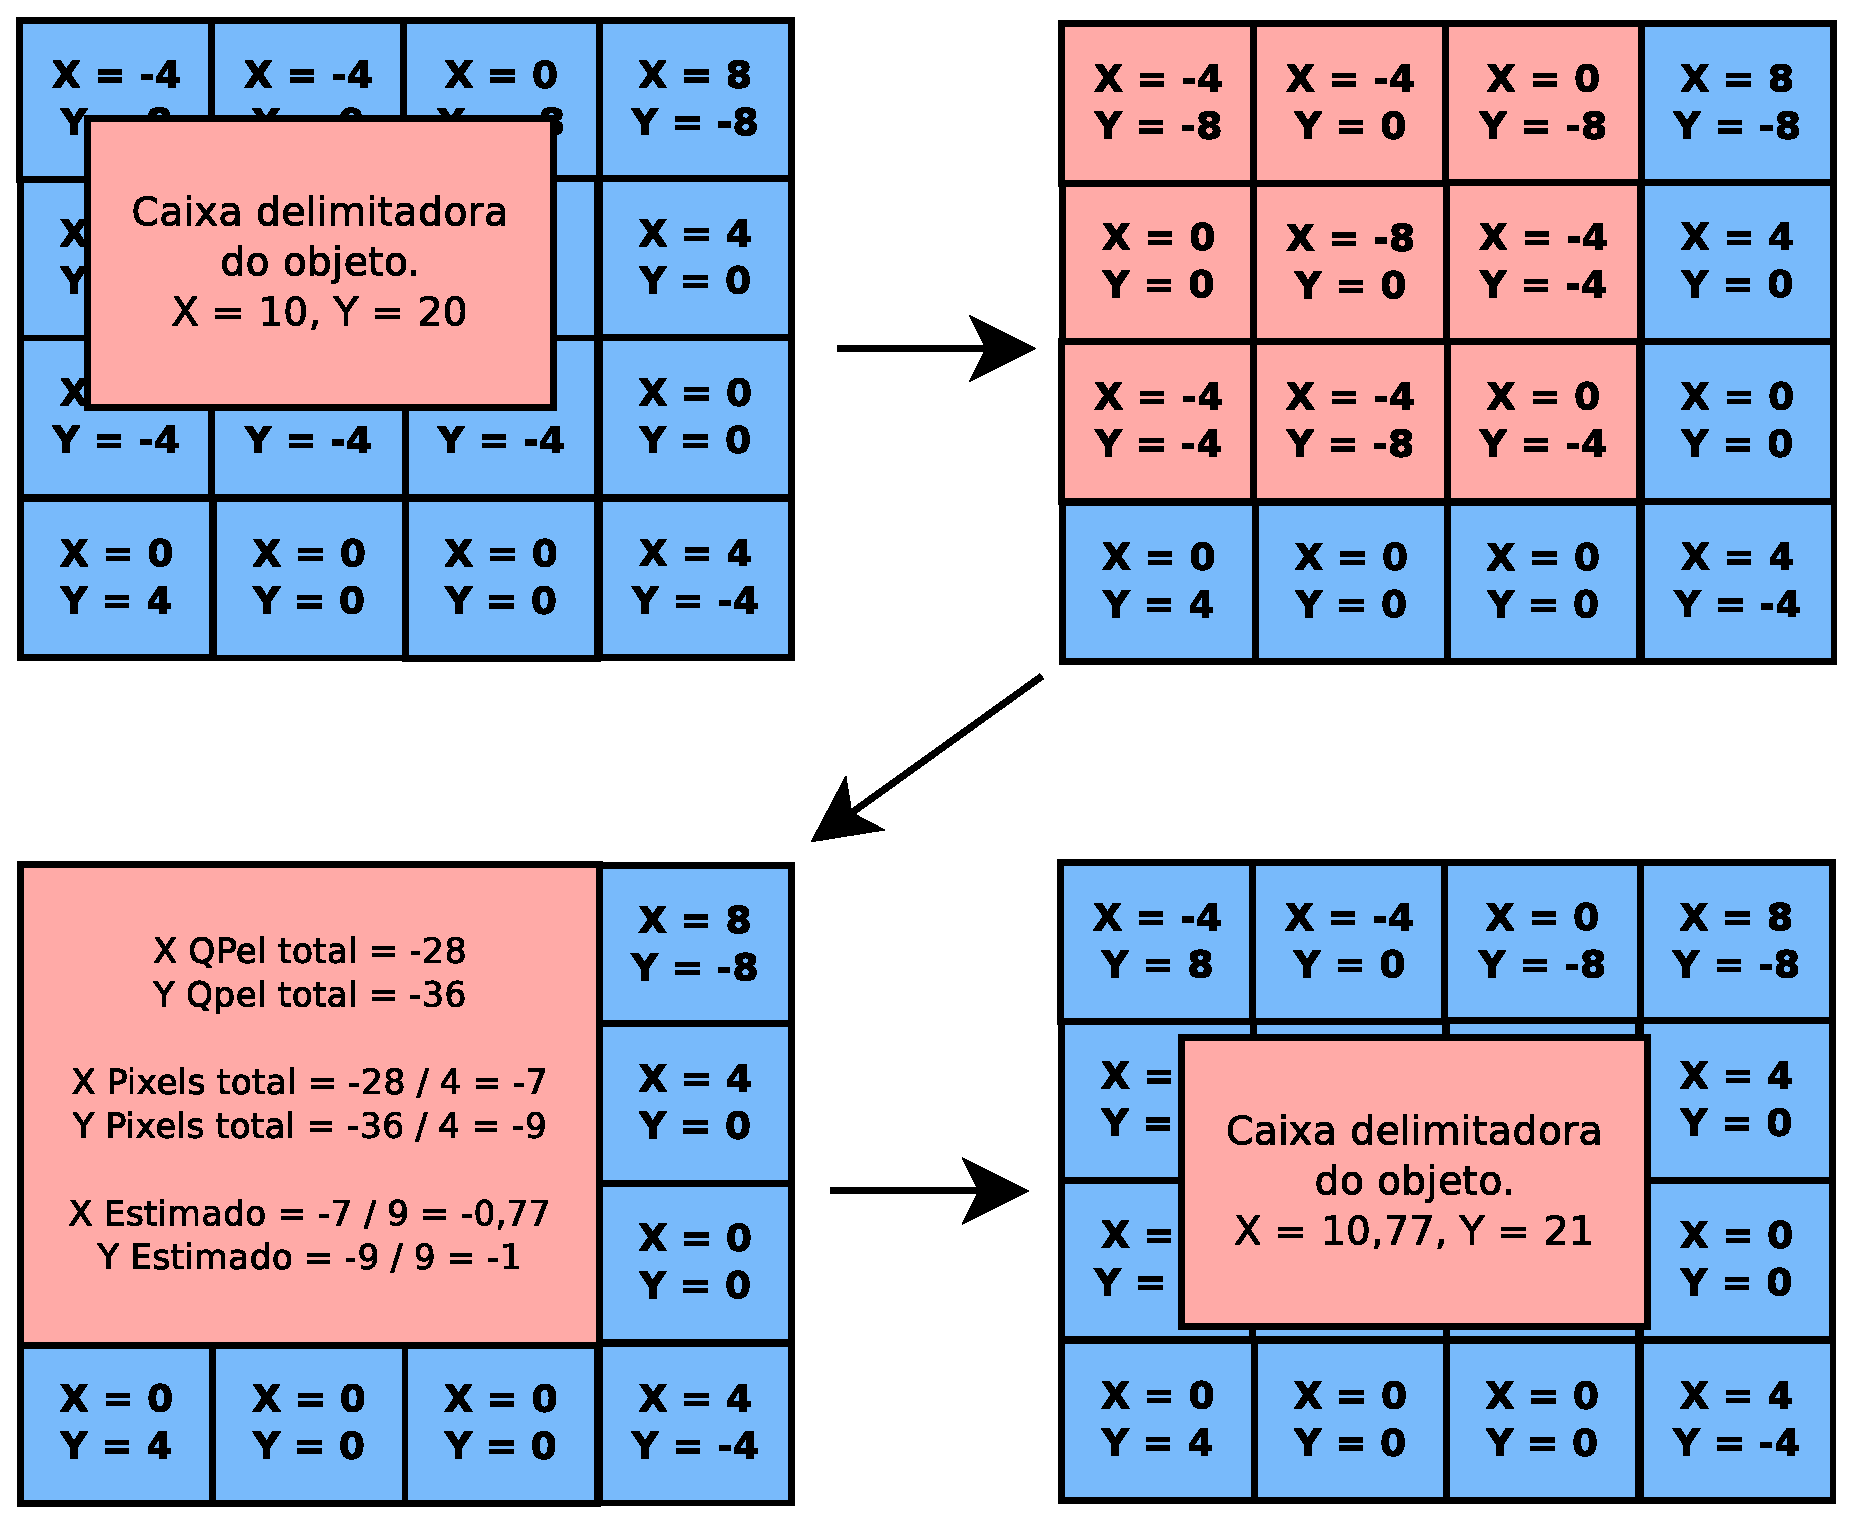
\includegraphics[scale=0.45]{imagens/fig17.eps}
\caption{Estimativa de movimento de um objeto.}
\label{fig:object_motion_estimation_example}
\end{figure}


Esse processo pode ser visto em detalhes no método \textit{estimate\_motion} da classe \textit{TrackedBoundingBox} que se encontra implementado em \textit{/lencod/src/metadata\_extractor.c}. 


\section{ Alterações realizadas no codificador }


O objetivo da criação dos módulos \textit{metadata\_extractor} e \textit{extracted\_metadata} foi reduzir ao máximo as alterações que teriam de ser realizadas no codificador e no decodificador e desacoplando o processo de extração de metadados do software de referência. Isso facilita a possibilidade de portar o sistema de detecção e \textit{tracking} de objetos para uma outra implementação do H264.

Nesta seção serão apresentadas as alterações realizadas no codificador do software de referência, para integrá-lo com os módulos construídos. As alterações realizadas no codificador se encontram no anexo A.


\begin{figure}[H]
\centering
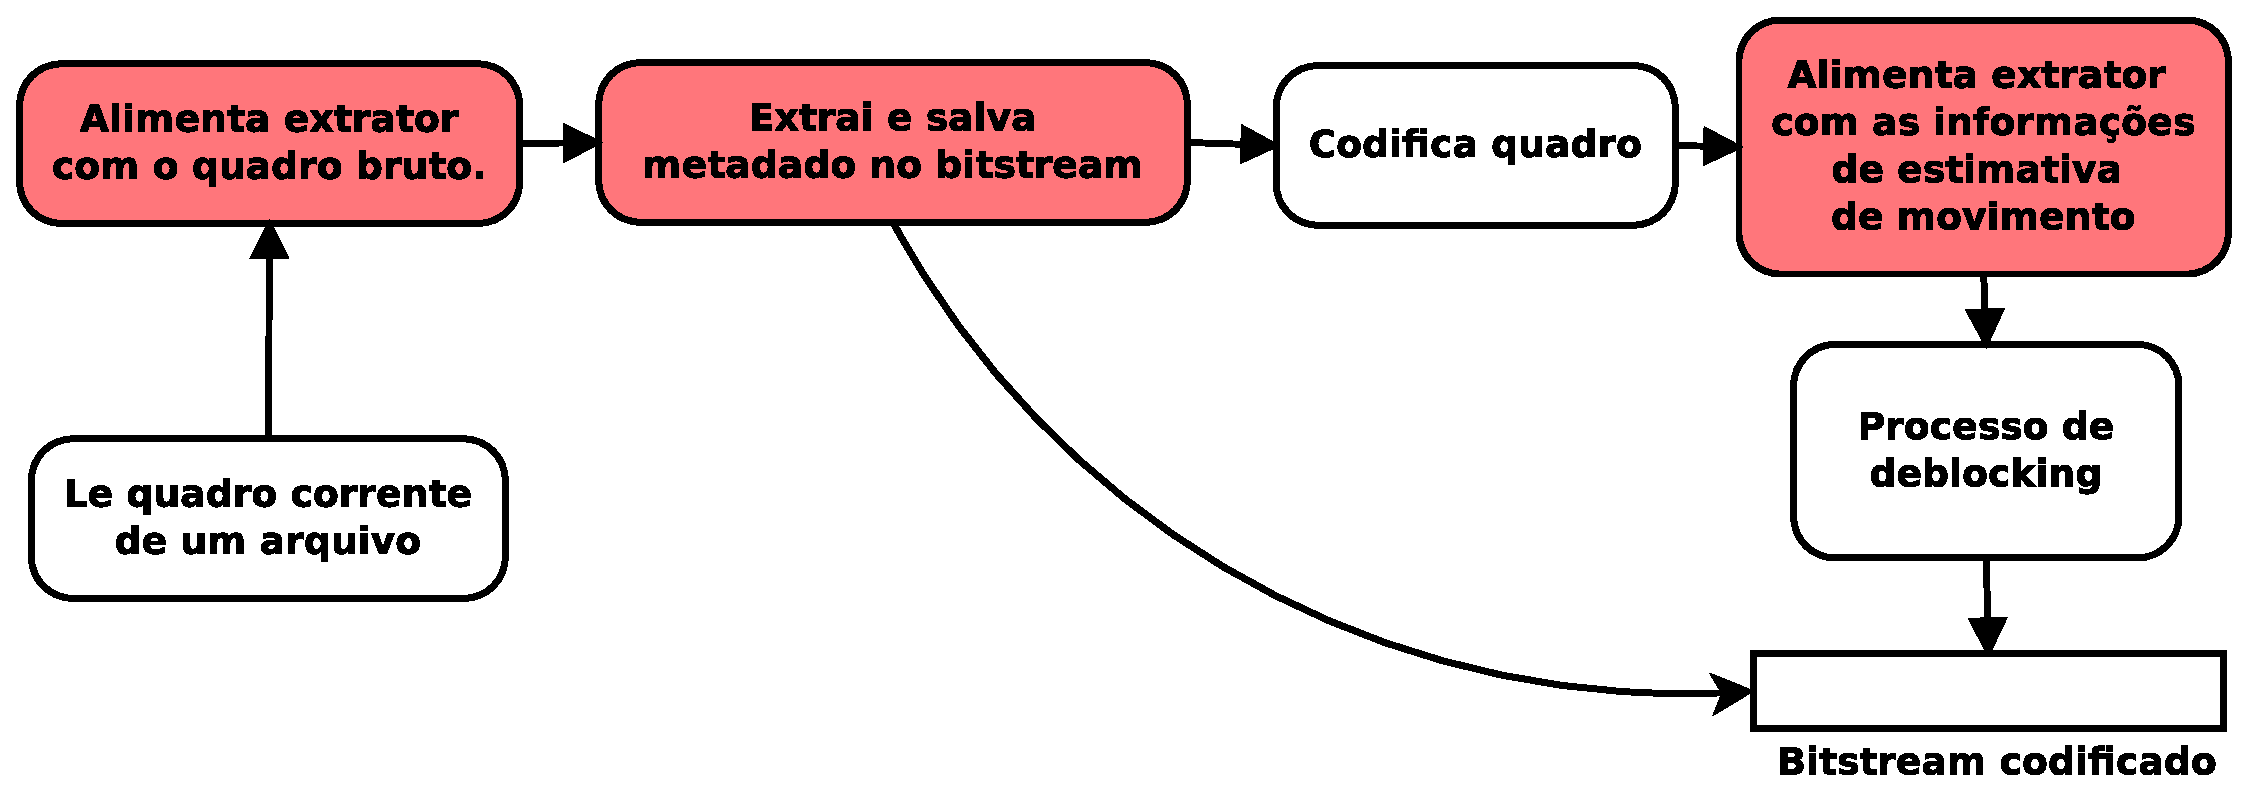
\includegraphics[scale=0.45]{imagens/fig18.eps}
\caption{Visão geral do codificador H.264 modificado. Os blocos vermelhos representam os processos adicionados ao codificador.}
\label{fig:h264_moded_encoder}
\end{figure}


\subsection{ Processando o quadro bruto }

Para extrair metadados do quadro bruto antes de ocorrer o processo de codificação, foi necessário primeiro descobrir qual o melhor local dentro do codificador para se obter o quadro que vai ser codificado. No caso do software de referência utilizado neste trabalho a entrada de dados é feita por arquivo. Foi necessário estudar quando o codificador lê o quadro e como ele organiza este quadro na memória.

A partir da função \textit{main} em \textit{lencod/src/lencod.c}, analisando como o codificador procedia para codificar os quadros, foi encontrada uma chamada para a função \textit{encode\_one\_frame}, esta função é implementada no módulo \textit{lencod/src/image.c}, é nesta função que o quadro é carregado em memória e pré-processado.

Dentro da função \textit{encode\_one\_frame}, o processamento do quadro bruto é realizado logo após a chamada de função \textit{process\_image}, que realiza o processamento final em cima do quadro bruto, antes de se iniciar a codificação dele. É neste ponto que o método \textit{extract\_object\_bounding\_box} é chamado e o metadado extraído é salvo no bitstream na forma de mensagem SEI \textit{Unregistered Userdata}, utilizando o módulo \textit{udata\_gen}.

\begin{lstlisting}

process_image(p_Vid, p_Inp);

if (p_Inp->object_detection_enable) {
    
  ExtractedMetadata * metadata = metadata_extractor_extract_object_bounding_box(p_Vid->metadata_extractor, p_Vid->frame_no, (unsigned char **) p_Vid->imgData.frm_data[0], p_Vid->imgData.format.width[0], p_Vid->imgData.format.height[0]);

  if (metadata) {
    int size                = extracted_metadata_get_serialized_size(metadata);
    char * data             = malloc(size);
    NALU_t * nalu           = NULL;
     
    /* Serialize the metadata */
    extracted_metadata_serialize(metadata, data);
      
    /* Insert the serialized metadata on the bitstream as SEI NALU. */
    nalu = user_data_generate_unregistered_sei_nalu(data, size);
    p_Vid->WriteNALU (p_Vid, nalu);

    FreeNALU (nalu);
    free(data);
    extracted_metadata_free(metadata);
  }

}

pad_borders (p_Inp->output, p_Vid->width, p_Vid->height, p_Vid->width_cr, p_Vid->height_cr, p_Vid->imgData.frm_data);

\end{lstlisting}

Tendo encontrado um bom lugar para extrair as informações foi necessário entender como o quadro fica organizado na memória. A estrutura \textit{ImageData} armazena as informações de um quadro, e o quadro original é carregado no campo \textit{imgdata} da estrutura \textit{VideoParameters}. A definição da estrutura \textit{ImageData} se encontra no módulo \textit{lcommon/inc/io\_image.h} e a estrutura \textit{VideoParameters} é definida em \textit{lencod/inc/global.h}.

O quadro original carregado se encontra no campo \textit{frm\_data} da estrutura \textit{ImageData}:

\begin{lstlisting}

typedef struct image_data
{
  FrameFormat format;               //!< image format
  // Standard data
  imgpel **frm_data[MAX_PLANE];     //!< Frame Data
  imgpel **top_data[MAX_PLANE];     //!< pointers to top field data
  imgpel **bot_data[MAX_PLANE];     //!< pointers to bottom field data

  //! Optional data (could also add uint8 data in case imgpel is of type uint16)
  //! These can be useful for enabling input/conversion of content of different types
  //! while keeping optimal processing size.
  uint16 **frm_uint16[MAX_PLANE];   //!< optional frame Data for uint16
  uint16 **top_uint16[MAX_PLANE];   //!< optional pointers to top field data
  uint16 **bot_uint16[MAX_PLANE];   //!< optional pointers to bottom field data

  int frm_stride[MAX_PLANE];
  int top_stride[MAX_PLANE];
  int bot_stride[MAX_PLANE];
} ImageData;

\end{lstlisting}

Este campo é um array tri-dimensional de \textit{imgpel}, o tipo \textit{imgpel} representa o tamanho de cada pixel e é definido no módulo \textit{lcommon/inc/typedefs.h}:

\begin{lstlisting}

#if (IMGTYPE == 0)
typedef byte   imgpel;           //!< pixel type
typedef uint16 distpel;          //!< distortion type (for pixels)
typedef int32  distblk;          //!< distortion type (for Macroblock)
typedef int32  transpel;         //!< transformed coefficient type
#elif (IMGTYPE == 2)
typedef float imgpel;
typedef float distpel;
typedef float distblk;
typedef int32 transpel;
#else
typedef uint16 imgpel;
typedef uint32 distpel;
typedef int64  distblk;
typedef int32  transpel;
#endif

\end{lstlisting}

\textit{IMGTYPE} é o que define o tamanho do pixel, e pode ser definido tanto para o codificador como para o decodificador (cada um deles pode trabalhar com um tamanho de pixel diferente). No encoder a definição do \textit{IMGTYPE} se encontra em \textit{lencod/inc/defines.h} e do decodificador em \textit{ldecod/inc/defines.h}. Por padrão o software de referência vem com esse valor definido como 1, ou seja utiliza 16 bits para representar cada pixel.

Tanto o encoder como o decodificador foram alterados para trabalhar com 8 bits para representar cada pixel, já que utilizar 16 bits não trazia vantagem alguma na extração dos metadados, gerando um overhead desnecessário.

\textit{MAX\_PLANE} é o que define a quantidade de planos existentes no quadro, e pode ser definido tanto para o encoder como para o decodificador (cada um deles pode possuir uma quantidade de planos diferente). No encoder a definição do \textit{MAX\_PLANE} se encontra em \textit{lencod/inc/defines.h} e no decodificador em \textit{ldecod/inc/defines.h}. Por padrão o software de referência vem com esse valor definido como 3, ou seja existem 3 planos em cada quadro.

Normalmente existem duas maneiras de se representar uma imagem: intercalada e planar. No caso dos quadros carregados no software de referência a representação é planar, no array tridimensional a primeira dimensão é o plano, \textit{frm\_data[0]} é o plano Y, \textit{frm\_data[1]} é o plano U e \textit{frm\_data[2]} é o plano V.

A segunda dimensão é o y/vertical do plano. A terceira dimensão é o x/horizontal do plano. O comprimento e a altura de cada plano se encontra no campo \textit{format} da estrutura \textit{ImageData}, que é do tipo \textit{FrameFormat}. O índice 0 acessa o comprimento e altura do plano Y, o índice 1 acessa o comprimento e altura dos planos de cor (UV),  o tipo \textit{FrameFormat} é definido em \textit{lcommon/inc/frame.h}:

\begin{lstlisting}

typedef struct frame_format
{
  ColorFormat yuv_format;                    //!< YUV format (0=4:0:0, 1=4:2:0, 2=4:2:2, 3=4:4:4)
  ColorModel  color_model;                   //!< 4:4:4 format (0: YUV, 1: RGB, 2: XYZ)
  double      frame_rate;                    //!< frame rate
  int         width[3];                      //!< component frame width
  int         height[3];                     //!< component frame height    
  int         auto_crop_right;               //!< luma component auto crop right
  int         auto_crop_bottom;              //!< luma component auto crop bottom
  int         auto_crop_right_cr;            //!< chroma component auto crop right
  int         auto_crop_bottom_cr;           //!< chroma component auto crop bottom
  int         width_crop;                    //!< width after cropping consideration
  int         height_crop;                   //!< height after cropping consideration
  int         mb_width;                      //!< luma component frame width
  int         mb_height;                     //!< luma component frame height    
  int         size_cmp[3];                   //!< component sizes (width * height)
  int         size;                          //!< total image size (sum of size_cmp)
  int         bit_depth[3];                  //!< component bit depth  
  int         max_value[3];                  //!< component max value
  int         max_value_sq[3];               //!< component max value squared
  int         pic_unit_size_on_disk;         //!< picture sample unit size on storage medium
  int         pic_unit_size_shift3;          //!< pic_unit_size_on_disk >> 3
} FrameFormat;

\end{lstlisting}

Para observar em mais detalhes como trabalhar com a estrutura \textit{ImageData} as funções \textit{MuxImages} e \textit{FilterImageSep} no módulo \textit{lcommon/src/img\_process.c} são bons exemplos.


\subsection{ Obtendo estimativa de movimento }


Além dos quadros brutos, outra informação importante para o extrator de metadados são os vetores de movimento dos blocos.

Na função \textit{code\_a\_plane} antes da chamada de função \textit{DeblockFrame} todo o processo de estimativa de movimento já está completo, e todos os vetores de movimento para todos os blocos da imagem estão disponíveis. Neste ponto é que os vetores de estimativa de movimento do quadro são repassados ao extrator de metadados para que ele realize a estimativa de movimento do objeto detectado (se o extrator estiver realizando \textit{tracking}).

Os vetores se encontram na estrutura \textit{VideoParameters} (definida em \textit{lencode/inc/global.h}) no campo \textit{enc\_picture} que é do tipo \textit{struct storable\_picture}. Sua definição se encontra em \textit{lencode/inc/mbuffer.h}, essa estrutura possui o campo \textit{mv\_info} que é um array bidimensional de \textit{PicMotionParams}.

A primeira dimensão é y do bloco, que vai de 0 até (altura da imagem / tamanho do bloco). A segunda dimensão é o x do bloco, que vai de 0 até (comprimento da imagem / tamanho do bloco). Ao acessar as duas dimensões temos o \textit{PicMotionParams} que possui os vetores de movimento para o bloco[y][x]. A estrutura \textit{PicMotionParams} é definida em \textit{lencode/inc/mbuffer.h} da seguinte maneira:

\begin{lstlisting}
//! definition of pic motion parameters
typedef struct pic_motion_params
{
  struct storable_picture *ref_pic[2];  //!< referrence picture pointer
  char                     ref_idx[2];  //!< reference picture   [list][subblock_y][subblock_x]
  MotionVector             mv[2];       //!< motion vector  
  byte                     field_frame; //!< indicates if co_located is field or frame. Will be removed at some point
} PicMotionParams;

\end{lstlisting}


O campo \textit{mv} possui dois vetores de movimento, a posição 0 tem os vetores de movimento calculados utilizando a lista 0, a posição 1 tem os vetores calculados utilizando a lista 1. Na implementação atual foram utilizados apenas os vetores de movimento da lista 0. Exemplo do código necessário para varrer todos os vetores de movimento da lista 0:


\begin{lstlisting}

int blk_y, blk_x;
  
for (blk_y=0; blk_y  < ceil(p_Vid->height / BLOCK_SIZE); blk_y++)
{

  for(blk_x = 0 ; blk_x < ceil(p_Vid->width / BLOCK_SIZE); blk_x++) {

    PicMotionParams *mv_info_p = &p_Vid->enc_picture->mv_info[blk_y][blk_x];

    printf("Vetor de movimento X da lista 0 para o bloco[%d][%d] = %d\n", blk_y, blk_x, mv_info_p->mv[LIST_0].mv_x);
    printf("Vetor de movimento Y da lista 0 para o bloco[%d][%d] = %d\n", blk_y, blk_x, mv_info_p->mv[LIST_0].mv_y);

  }

}

\end{lstlisting}


Exemplos mais completos para entender como trabalhar com os vetores de movimento no software de referência se encontram nas funções da família \textit{GetStrength} que se encontram nas diferentes implementações de \textit{loop\_filter} (ex. \textit{loop\_filter\_normal.c}).


\subsection{ Configurações adicionadas ao codificador }


Foram adicionadas novas configurações no codificador do software de referência, para controlar melhor o processo de detecção de objetos. As configurações primeiro têm de ser adicionadas à estrutura \textit{struct inp\_par\_enc}, que se encontra em \textit{lcommon/inc/params.h}. Os campos adicionados foram:

\begin{itemize}
	\item object\_detection\_enable - Habilita ou desabilita a detecção de objetos.
        \item object\_detection\_min\_width - Comprimento mínimo do objeto para que ele seja detectado.
        \item object\_detection\_min\_height - Altura mínima do objeto para que ele seja detectado.
        \item object\_detection\_search\_hysteresis - Histerese (em quadros) da busca de um novo objeto.
        \item object\_detection\_tracking\_hysteresis - Histerese (em quadros) para confirmar a existência/posição de um objeto que está sendo feito \textit{tracking}.
	\item object\_detection\_training\_file - Arquivo de treinamento do classificador Haar, define o objeto que será detectado.
\end{itemize}

Essas configurações também foram adicionadas na estrutura \textit{Map} que se encontra em \textit{lencod/inc/configfile.h}. Tendo feito isso o software de referência automaticamente carregará essas configurações com os valores default definidos na estrutura \textit{Map} e tentará obter esses campos a partir do arquivo de configuração que é informado ao executar o codificador através da opção -f. Os valores definidos no arquivo de configuração são automaticamente carregados na estrutura \textit{InputParameters}.

Um exemplo de como definir essas configurações no arquivo de configuração:

\begin{lstlisting}

##########################################################################################
# Object detection/tracking configuration
##########################################################################################
object_detection_enable              = 1  # 1 = Enable, 0 = Disable
object_detection_min_width           = 30 # Min width of the object that will be detected
object_detection_min_height          = 30 # Min height of the object that will be detected
object_detection_search_hysteresis   = 10 # Search for new object hysteresys (in frames).
object_detection_tracking_hysteresis = 30 # Confirm tracked object existence hysteresis (in frames).
object_detection_training_file       = "haarcascade_frontalface_alt.xml" #File containing the training info used on the object detection.

\end{lstlisting}


\section{ Alterações realizadas no Decodificador }


Nesta seção serão apresentadas as alterações realizadas no decodificador do software de referência, para aplicar os metadados recebidos no vídeo decodificado. As alterações visam desenhar nos quadros decodificados os metadados do tipo \textit{ExtractedObjectBoundingBox} presentes no bitstream, facilitando a constatação visual da eficácia do sistema de detecção e \textit{tracking} de objetos implementados no codificador. Para simplificar a implementação do decodificador ele só detecta e aplica um metadado por quadro, mas não existe algo que impossibilite a aplicação de vários metadados em cada quadro.

As alterações se concentram no momento em que um NALU do tipo SEI \textit{Unregistered UserData} é detectado no bitstream, e um pouco antes do quadro decodificado ser gravado no arquivo de saída configurado. As alterações realizadas no decodificador se encontram no anexo B.

\begin{figure}[H]
\centering
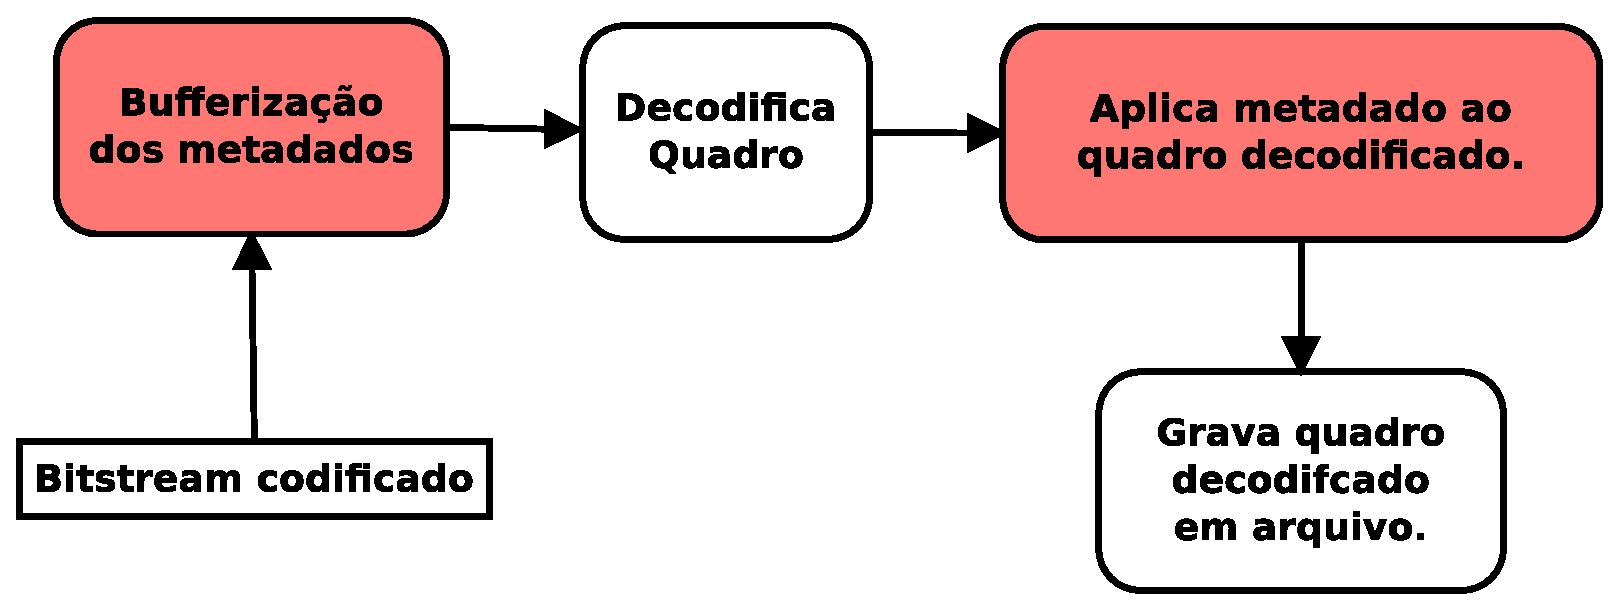
\includegraphics[scale=0.5]{imagens/fig19.eps}
\caption{Visão geral do decodificador H.264 modificado. Os blocos vermelhos representam os processos adicionados ao decodificador.}
\label{fig:h264_moded_decoder}
\end{figure}


\subsection{ Recuperando metadados a partir do bitstream }


Para realizar a recuperação de um metadado previamente inserido no bitstream durante o processo de codificação foi adicionado na estrutura \textit{VideoParameters} (definida em \textit{ldecod/inc/global.h}) do decodificador um novo campo chamado \textit{metadata\_buffer} do tipo \textit{ExtractedMetadataBuffer}. Esse buffer é inicializado na função \textit{main} do decodificador, que se encontra em \textit{ldecod/src/decoder\_test.c}, logo após o decodificador ter sido configurado, mas antes de iniciar o processo de decodificação.

Ao longo do processo de decodificação, sempre que um NALU do tipo SEI é encontrado no bitstream a função \textit{InterpretSEIMessage} é chamada, essa função se encontra em \textit{ldecod/src/sei.c}. Nela existe um \textit{switch case} para os diversos tipos de mensagens SEI possíveis, no \textit{case} \textit{SEI\_USER\_DATA\_UNREGISTERED} foi adicionada detecção se essa mensagem é um \textit{ExtractedMetadata}. Em caso afirmativo, esse metadado será adicionado ao \textit{ExtractedMetadataBuffer}, caso contrário a mensagem é ignorada.


\subsection{ Aplicando o metadado ao quadro }


Depois de receber e bufferizar os metadados foi necessário encontrar um bom lugar para aplicar os metadados ao quadro, de preferência logo antes do quadro ser gravado em arquivo, onde todo o processo de decodificação já teria ocorrido. Foi escolhido o inicio da função \textit{write\_out\_picture}, que se encontra em \textit{ldecod/src/output.c} como melhor local para realizar a aplicação do metadado.

Para auxiliar o processo de aplicação de metadados do tipo \textit{ExtractedObjectBoundingBox} foi adicionado em \textit{ldecod/src/output.c} a função \textit{decoder\_draw\_bounding\_box}, que verifica se o metadado é do tipo \textit{ExtractedObjectBoundingBox}, em caso afirmativo a caixa delimitadora é desenhada no quadro, caso contrário o metadado é ignorado.

No inicio da função \textit{write\_out\_picture} um contador é utilizado para definir o número do quadro (em ordem de apresentação), o número do quadro é utilizado na chamada do método \textit{get} da classe \textit{ExtractedMetadataBuffer}, para verificar a existência de um metadado para aquele quadro. Se um metadado existir para este quadro, será chamada a função \textit{decoder\_draw\_bounding\_box}, que desenhará a caixa delimitadora no quadro.



\chapter{ Testes }

Neste capítulo são apresentados os testes realizados no sistema proposto, integrando o classificador Haar ao codificador do H.264. Testes detalhados de desempenho comparando o classificador Haar do OpenCV com outros 2 algoritmos de detecção de objetos, podem ser vistos em \cite{haarTests}. Todos os testes utilizaram o mesmo arquivo de treinamento \textit{haarcascade\_frontalface\_alt.xml}, que realiza a busca de faces frontais, este arquivo vem junto com a distribuição do OpenCV (que pode ser encontrada em http://sourceforge.net/projects/opencvlibrary/files) no diretório \textit{data/haarcascades}. O tamanho mínimo do objeto de interesse configurado em todos os testes foi de 30 x 30 pixels.

A configuração da máquina e o sistema operacional utilizados nos testes foi:


\begin{itemize}
        \item Processador Pentium(R) Dual-Core E5200 á 2.50GHz.
        \item 4 gigabytes de memória RAM.
        \item Sistema operacional Ubuntu 11.04 32 bits.
\end{itemize}


Os parâmetros medidos foram os seguintes:

\begin{itemize}
        \item Desempenho do sistema com \textit{tracking} de objetos X sem \textit{tracking} de objetos.
	\item Desempenho do sistema com o uso de histerese X sem o uso de histerese.
        \item Desempenho do sistema com diferentes configurações de histerese.
	\item Qualidade do \textit{tracking} de objetos em suas diferentes configurações, constatando visualmente a caixa delimitadora desenhada no vídeo.
	\item Tamanho do bitstream com \textit{tracking} de objetos X sem \textit{tracking} de objetos.
\end{itemize}


Foram realizados 5 testes em cada vídeo:


\begin{itemize}
        \item Sem \textit{tracking} de objetos.

	\item Com \textit{tracking} ativado, com histerese de busca = 1 e histerese de \textit{tracking} = 1. Dessa maneira as informações de estimativa de movimento do codificador não são utilizadas, o \textit{tracking} é realizado utilizando apenas o classificador Haar.

	\item Com \textit{tracking} ativado, com histerese de busca = 5 e histerese de \textit{tracking} = 10. Essa configuração faz um menor uso das informações de estimativa de movimento para realizar \textit{tracking} de um objeto.

         \item Com \textit{tracking} ativado, com histerese de busca = 10 e histerese de \textit{tracking} = 30. Essa configuração depende mais das informações de estimativa de movimento para realizar \textit{tracking} de um objeto.

         \item Com \textit{tracking} ativado, com histerese de busca = 10 e histerese de \textit{tracking} = 60. Essa configuração é a que mais depende mais das informações de estimativa de movimento para realizar \textit{tracking} de um objeto.
\end{itemize}


Dessa maneira é possível avaliar a diferença entre realizar o \textit{tracking} de um objeto utilizando apenas o classificador Haar, ou utilizando histereses com auxílio das informações de estimativa de movimento. Em todos os testes foi utilizada a mesma configuração de codificação, a única diferença entre as configurações são o arquivo de origem, arquivo de destino, resolução e taxa de apresentação (pois esses parâmetros são diferentes para cada vídeo). No apêndice E encontram-se as configurações que foram alteradas a partir do arquivo de configuração original que vem junto com o software de referência (o arquivo de configuração original se encontra em \textit{bin/encoder.cfg}).


\section{ Vídeo Akiyo - QCIF - 300 quadros }


Esse vídeo pode ser encontrado em http://media.xiph.org/video/derf/y4m/akiyo\_qcif.y4m e consiste basicamente de 300 quadros positivos (existe o objeto de interesse ao longo de todo o vídeo, nesse caso uma face frontal).


Especificações do vídeo:

\begin{itemize}
        \item quadros por segundo = 29.97.
        \item total de quadros    = 300.
        \item comprimento         = 176 pixels.
        \item altura              = 144 pixels.
        \item espaço de cor       = YUV, 4:2:0.
\end{itemize}


\begin{table}[H]
\begin{center}
\begin{tabular}{|p{2.3cm}|p{2.3cm}|p{2.3cm}|p{2.3cm}|p{2.3cm}|p{2.3cm}|}
\hline
\textbf{} & \textbf{\textit{Tracking} Desabilitado} & \textbf{\textit{Tracking} habilitado, sem histerese} & \textbf{Histerese de busca = 5, \textit{tracking} = 10} & \textbf{Histerese de busca = 10, \textit{tracking} = 30} & \textbf{Histerese de busca = 10, \textit{tracking} = 60} \\
\hline
Tempo Total de Codificação (segundos) & 35,053 & 38,889 & 35,500 & 35,260 & 35,190 \\
\hline
Tamanho bitstream (bytes) & 359220 & 372974 & 372790 & 372560 & 372561 \\
\hline
Atraso no tempo total codificação & 0\% & 10,94\% & 1,27\% & 0,59\% & 0,39\% \\
\hline
Aumento bitstream  & 0\% & 3,83\% & 3,77\% & 3,71\% & 3,71\% \\
\hline
\end{tabular}
\caption{Desempenho do sistema com o vídeo Akiyo.}
\label{tab:space_overhead}
\end{center}
\end{table}

\begin{figure}[H]
\centering
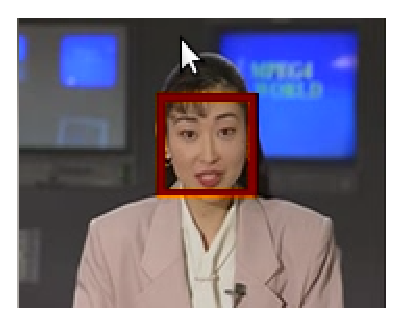
\includegraphics[scale=0.8]{imagens/fig20.eps}
\caption{Face detectada no vídeo Akiyo.}
\label{fig:akiyo_example}
\end{figure}

Como este vídeo é composto de apenas uma pessoa, realizando pequenos movimentos suaves, os resultados com histerese de \textit{tracking} alta foram bons. A ativação de detecção de objetos em todos os quadros, utilizando apenas o classificador Haar para realizar o \textit{tracking}, tornou o processo de codificação aproximadamente 10,94\% mais lento. 

A utilização do classificador Haar em conjunto com a estimativa de movimento fez com que a caixa delimitadora realizasse movimentos mais suaves, com um atraso variando de 1,27\% á 0,39\% em relação ao processo de codificação original, dependendo da configuração da histerese. O aumento no bitstream no pior caso foi de 3,83\%.

Em todos as configurações a qualidade do vídeo codificado mostrou ser a mesma:

\begin{lstlisting}

Y { PSNR (dB), cSNR (dB), MSE }   : {  41.348,  39.978,   6.53497 }
U { PSNR (dB), cSNR (dB), MSE }   : {  49.603,  49.132,   0.79417 }
V { PSNR (dB), cSNR (dB), MSE }   : {  51.103,  51.031,   0.51284 }

Total bits                        : 2873760 (I 1944040, P 929560, NVB 160) 
Bit rate (kbit/s)  @ 30.00 Hz     : 287.38
Bits to avoid Startcode Emulation : 0 
Bits for parameter sets           : 160 
Bits for filler data              : 0

\end{lstlisting}


\section{ Vídeo \textit{Coast guard} - QCIF - 300 quadros }


Esse vídeo pode ser encontrado em http://media.xiph.org/video/derf/y4m/coastguard\_qcif.y4m e consiste basicamente de 300 quadros negativos (não existe o objeto de interesse ao longo de todo o vídeo). Como a histerese de \textit{tracking} não é utilizada neste teste, a configuração com histerese de busca de 10 quadros e histerese de \textit{tracking} de 60 quadros não será apresentada.


Especificações do vídeo:

\begin{itemize}
        \item quadros por segundo = 29.97.
        \item total de quadros    = 300.
        \item comprimento         = 176 pixels.
        \item altura              = 144 pixels. 
        \item espaço de cor       = YUV, 4:2:0.
\end{itemize}


\begin{table}[H]
\begin{center}
\begin{tabular}{|p{2.3cm}|p{2.3cm}|p{2.3cm}|p{2.3cm}|p{2.3cm}|}
\hline
\textbf{} & \textbf{\textit{Tracking} Desabilitado} & \textbf{\textit{Tracking} habilitado, sem histerese} & \textbf{Histerese de busca = 5, \textit{tracking} = 10} & \textbf{Histerese de busca = 10, \textit{tracking} = 30}  \\
\hline
Tempo Total de Codificação (segundos) & 78,200 & 84,800 & 79,482 & 78,896  \\
\hline
Tamanho bitstream (bytes) & 1240200 & 1240200 & 1240200 & 1240200  \\
\hline
Atraso no tempo total codificação & 0\% & 8,43\% & 1,63\% & 0,89\%  \\
\hline
Aumento bitstream  & 0\% & 0\% & 0\% & 0\%  \\
\hline
\end{tabular}
\caption{Desempenho do sistema com o vídeo Coast Guard.}
\label{tab:space_overhead}
\end{center}
\end{table}


A ativação de detecção de objetos em todos os quadros tornou o processo de codificação aproximadamente 8,43\% mais lento. A utilização do classificador Haar com histerese de busca de 10 quadros gerou bons resultados, um atraso de apenas 0,89\% em relação ao processo de codificação original. Com uma histerese de busca de 5 quadros o atraso dobrou para 1,63\%, ainda sendo um valor bem inferior ao atraso gerado pelo processamento de todos os quadros. Como esse vídeo não possui nenhum objeto de interesse o bitstream teve o mesmo tamanho em todas as configurações, e a histerese de \textit{tracking} não foi nem sequer utilizada.


Em todos as configurações a qualidade do vídeo codificado mostrou ser a mesma:

\begin{lstlisting}

Y { PSNR (dB), cSNR (dB), MSE }   : {  36.174,  34.758,  21.73983 }
U { PSNR (dB), cSNR (dB), MSE }   : {  47.488,  46.834,   1.34807 }
V { PSNR (dB), cSNR (dB), MSE }   : {  49.023,  48.567,   0.90448 }

Total bits                        : 9921600 (I 3033832, P 6887608, NVB 160) 
Bit rate (kbit/s)  @ 29.97 Hz     : 991.17
Bits to avoid Startcode Emulation : 0 
Bits for parameter sets           : 160 
Bits for filler data              : 0 

\end{lstlisting}



\section{ Vídeo \textit{Crew} - CIF - 300 quadros }


Esse vídeo pode ser encontrado em http://media.xiph.org/video/derf/y4m/crew\_cif.y4m, possui várias pessoas andando juntas, possuindo diversas faces frontais em uma boa parte do vídeo, andando na direção da câmera (efeito de \textit{zoom}), até que as faces ficam de perfil.


Especificações do vídeo:

\begin{itemize}
        \item quadros por segundo = 29.97.
        \item total de quadros    = 300.
        \item comprimento         = 352 pixels.
        \item altura              = 288 pixels.
        \item espaço de cor       = YUV, 4:2:0.
\end{itemize}


\begin{table}[H]
\begin{center}
\begin{tabular}{|p{2.3cm}|p{2.3cm}|p{2.3cm}|p{2.3cm}|p{2.3cm}|p{2.3cm}|}
\hline
\textbf{} & \textbf{\textit{Tracking} Desabilitado} & \textbf{\textit{Tracking} habilitado, sem histerese} & \textbf{Histerese de busca = 5, \textit{tracking} = 10} & \textbf{Histerese de busca = 10, \textit{tracking} = 30} & \textbf{Histerese de busca = 10, \textit{tracking} = 60} \\
\hline
Tempo Total de Codificação (segundos) & 341,362 & 371,870 & 344,997 & 342,596 & 342,376 \\
\hline
Tamanho bitstream (bytes) & 1245195 & 1255323 & 1256008 & 1256661 & 1257621 \\
\hline
Atraso no tempo total codificação & 0\% & 8,93\% & 1,06\% & 0,36\% & 0,29\% \\
\hline
Aumento bitstream  & 0\% & 0,81\% & 0,86\% & 0,92\% & 0,99\% \\
\hline
\end{tabular}
\caption{Desempenho do sistema com o vídeo Crew.}
\label{tab:space_overhead}
\end{center}
\end{table}


\begin{figure}[H]
\centering
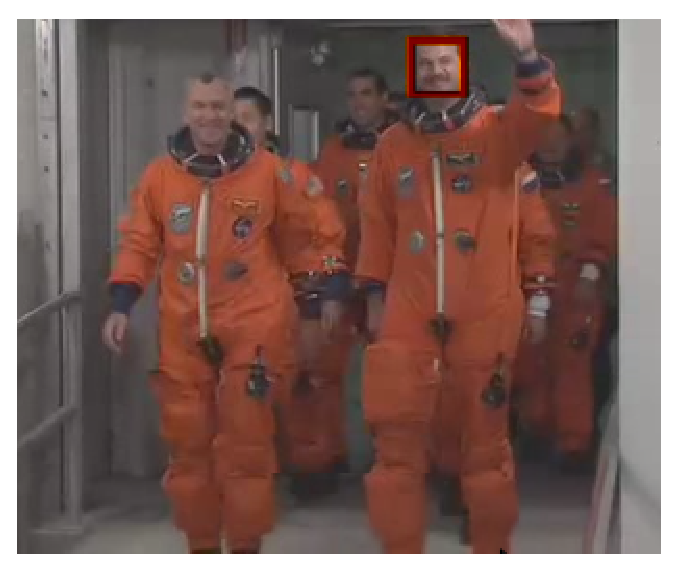
\includegraphics[scale=0.6]{imagens/fig22.eps}
\caption{Face detectada no vídeo \textit{Crew}.}
\label{fig:crew_example}
\end{figure}


Como este vídeo é composto de várias pessoas andando juntas, possui diversas faces frontais simultaneamente. Dessa maneira ele exibe duas limitações do sistema, a capacidade de detectar e realizar o tracking de apenas um objeto por vez (é possível realizar o \textit{tracking} de vários objetos diferentes, utilizando extratores com treinamentos diferentes, mas não o \textit{tracking} de vários objetos com mesma forma), e algumas falhas quando um objeto se move rápido demais (a caixa delimitadora se move mais lentamente que o objeto). 

Quanto ao desempenho a ativação de detecção de objetos em todos os quadros tornou o processo de codificação 8,93\% mais lento. A utilização do classificador Haar em conjunto com a estimativa de movimento diminui consideravelmente o custo computacional, com um atraso no processo de codificação variando entre 1,06\% e 0,29\% em relação ao processo de codificação original. O bitstream com os metadados inseridos no pior caso ficou 0,99\% maior que o bitstream original.


Em todos as configurações a qualidade do vídeo codificado mostrou ser a mesma:

\begin{lstlisting}
Y { PSNR (dB), cSNR (dB), MSE }   : {  35.790,  35.087,  20.15370 }
U { PSNR (dB), cSNR (dB), MSE }   : {  39.443,  38.836,   8.50048 }
V { PSNR (dB), cSNR (dB), MSE }   : {  38.490,  37.766,  10.87730 }

Total bits                        : 10000072 (I 2404808, P 7595096, NVB 168) 
Bit rate (kbit/s)  @ 30.00 Hz     : 1000.01
Bits to avoid Startcode Emulation : 0 
Bits for parameter sets           : 168 
Bits for filler data              : 0
\end{lstlisting}


\section{ Vídeo Foreman - CIF - 300 quadros }


Esse vídeo pode ser encontrado em http://media.xiph.org/video/derf/y4m/foreman\_cif.y4m e possui 3 situações diferentes, uma face frontal, a face fica de perfil em alguns momentos, e depois a face sai do vídeo.


Especificações do vídeo:

\begin{itemize}
        \item quadros por segundo = 29.97.
        \item total de quadros    = 300.
        \item comprimento         = 352 pixels.
        \item altura              = 288 pixels.
        \item espaço de cor       = YUV, 4:2:0.
\end{itemize}


\begin{table}[H]
\begin{center}
\begin{tabular}{|p{2.3cm}|p{2.3cm}|p{2.3cm}|p{2.3cm}|p{2.3cm}|p{2.3cm}|}
\hline
\textbf{} & \textbf{\textit{Tracking} Desabilitado} & \textbf{\textit{Tracking} habilitado, sem histerese} & \textbf{Histerese de busca = 5, \textit{tracking} = 10} & \textbf{Histerese de busca = 10, \textit{tracking} = 30} & \textbf{Histerese de busca = 10, \textit{tracking} = 60} \\
\hline
Tempo Total de Codificação (segundos) & 260,432 & 286,162 & 265,003 & 262,654 & 262,126 \\
\hline
Tamanho bitstream (bytes) & 1244893 & 1249485 & 1250345 & 1251793 & 1253161 \\
\hline
Atraso no tempo total codificação & 0\% & 9,87\% & 1,75\% & 0,85\% & 0,65\% \\
\hline
Aumento bitstream  & 0\% & 0,36\% & 0,43\% & 0,55\% & 0,66\% \\
\hline
\end{tabular}
\caption{Desempenho do sistema com o vídeo Foreman.}
\label{tab:space_overhead}
\end{center}
\end{table}

\begin{figure}[H]
\centering
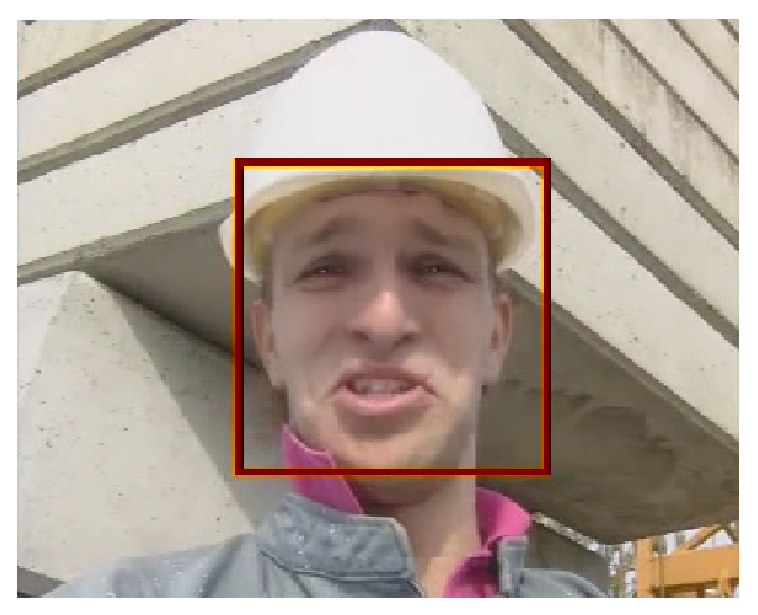
\includegraphics[scale=0.6]{imagens/fig21.eps}
\caption{Face detectada no vídeo Foreman.}
\label{fig:foreman_example}
\end{figure}

Com a detecção de objetos ocorrendo em todos os quadros percebe-se uma alta taxa de falsos negativos, já que o rosto no vídeo fica de perfil em alguns momentos e o classificador Haar não consegue identificar o rosto em perfil, perdendo assim o \textit{tracking} do rosto. Com a detecção de objetos em todos os quadros também ocorreu um falso positivo quando a câmera se move e deixa de gravar o rosto. A medida que a histerese de \textit{tracking} é aumentada, além de não ocorrer o falso positivo, os movimentos que o rosto realiza são acompanhados com maior suavidade e com uma menor taxa de falsos negativo (com a histerese de \textit{tracking} configurada para 60 quadros não ocorreu nenhum falso negativo). 

Quanto ao desempenho a ativação de detecção de objetos em todos os quadros tornou o processo de codificação 9,87\% mais lento. A utilização do classificador Haar em conjunto com a estimativa de movimento diminui consideravelmente o custo computacional, com um atraso no processo de codificação variando entre 1,75\% e 0,65\% em relação ao processo de codificação original. O bitstream com os metadados inseridos no pior caso ficou 0,66\% maior que o bitstream original.


Em todos as configurações a qualidade do vídeo codificado mostrou ser a mesma:

\begin{lstlisting}
Y { PSNR (dB), cSNR (dB), MSE }   : {  36.017,  34.568,  22.71311 }
U { PSNR (dB), cSNR (dB), MSE }   : {  41.277,  40.985,   5.18274 }
V { PSNR (dB), cSNR (dB), MSE }   : {  43.175,  42.592,   3.57977 }

Total bits                        : 9959144 (I 2813168, P 7145808, NVB 168) 
Bit rate (kbit/s)  @ 30.00 Hz     : 995.91
Bits to avoid Startcode Emulation : 0 
Bits for parameter sets           : 168 
Bits for filler data              : 0
\end{lstlisting}


\section{ Vídeo \textit{Pedestrian area} - 375 quadros }


Esse vídeo pode ser encontrado em http://media.xiph.org/video/derf/y4m/pedestrian\_area\_1080p25.y4m. Ele consiste basicamente de vários pedestres caminhando em uma rua, possui faces frontais e faces em perfil se movendo continuamente. 


\subsection{ Testes com resolução 1080p (1920 x 1080) }

Especificações do vídeo:

\begin{itemize}
        \item quadros por segundo = 25.
        \item total de quadros    = 375.
        \item comprimento         = 1920 pixels.
        \item altura              = 1080 pixels.
        \item espaço de cor       = YUV, 4:2:0.
\end{itemize}


\begin{table}[H]
\begin{center}
\begin{tabular}{|p{2.3cm}|p{2.3cm}|p{2.3cm}|p{2.3cm}|p{2.3cm}|p{2.3cm}|}
\hline
\textbf{} & \textbf{\textit{Tracking} Desabilitado} & \textbf{\textit{Tracking} habilitado, sem histerese} & \textbf{Histerese de busca = 5, \textit{tracking} = 10} & \textbf{Histerese de busca = 10, \textit{tracking} = 30} & \textbf{Histerese de busca = 10, \textit{tracking} = 60} \\
\hline
Tempo Total de Codificação (segundos) & 6915.861 & 7280.818 & 6921.871 & 6918.653 & 6916.272 \\
\hline
Tamanho bitstream (bytes) & 7854045 & 7870345 & 7870468 & 7870642 & 7870601 \\
\hline
Atraso no tempo total codificação & 0\% & 5,27\% & 0,08\% & 0,04\% & 0,005\% \\
\hline
Aumento bitstream  & 0\% & 0,207\% & 0,209\% & 0,211\% & 0,210\% \\
\hline
\end{tabular}
\caption{Desempenho do sistema com o vídeo \textit{Pedestrian area}.}
\label{tab:space_overhead}
\end{center}
\end{table}

\begin{figure}[H]
\centering
\includegraphics[scale=0.3]{imagens/fig25.eps}
\caption{Face detectada no vídeo \textit{Pedestrian area}.}
\label{fig:pedestrian_example}
\end{figure}

Com a detecção de objetos ocorrendo em todos os quadros ocorre uma grande quantidade de falsos positivos, e a limitação de realizar o \textit{tracking} de apenas um objeto por vez ficou bem evidente já que neste vídeo existem diversas pessoas andando ao mesmo tempo o sistema consegue realizar o \textit{tracking} de algumas faces por um curto período de tempo, mas logo depois detecta outra face e passa a realizar o \textit{tracking} dessa face ao invés da que foi previamente detectada. 

A utilização das histereses alterou um pouco o comportamento do sistema (em geral ele manteve uma alta taxa de falsos positivos), a primeira detecção que ocorre com sucesso realiza o \textit{tracking} da face corretamente, mas após essa primeira detecção ocorre uma série de falsos positivos, e em algumas detecções positivas o \textit{tracking} não consegue acompanhar a face por ela estar se movendo rápido demais.

Quanto ao desempenho a ativação de detecção de objetos em todos os quadros tornou o processo de codificação 5,27\% mais lento. A utilização do classificador Haar em conjunto com a estimativa de movimento diminui consideravelmente o custo computacional, com um atraso no processo de codificação inferior a 0,1\% em todas as configurações de histerese testadas. O bitstream com os metadados inseridos no pior caso ficou 0,211\% maior que o bitstream original.


Em todos as configurações a qualidade do vídeo codificado mostrou ser a mesma:

\begin{lstlisting}
Y { PSNR (dB), cSNR (dB), MSE }   : {  37.196,  37.136,  12.57412 }
U { PSNR (dB), cSNR (dB), MSE }   : {  41.390,  41.356,   4.75815 }
V { PSNR (dB), cSNR (dB), MSE }   : {  42.574,  42.530,   3.63104 }

Total bits                        : 62832360 (I 11049512, P 51782664, NVB 184) 
Bit rate (kbit/s)  @ 25.00 Hz     : 4188.82
Bits to avoid Startcode Emulation : 0 
Bits for parameter sets           : 184 
Bits for filler data              : 0
\end{lstlisting}


\subsection{ Testes com resolução 720p (1280 x 720) }


Neste teste a resolução do vídeo que foi reduzida de \textit{1080p} (1920 x 1080) para \textit{720p} (1280 x 720), visando a constatação da diferença do impacto do sistema de \textit{tracking} ao processar o mesmo vídeo com resoluções diferentes. O escalonamento do vídeo foi realizado utilizando o Gstreamer.


Especificações do vídeo:

\begin{itemize}
        \item quadros por segundo = 25.
        \item total de quadros    = 375.
        \item comprimento         = 1280 pixels.
        \item altura              = 720 pixels.
        \item espaço de cor       = YUV, 4:2:0.
\end{itemize}


\begin{table}[H]
\begin{center}
\begin{tabular}{|p{2.3cm}|p{2.3cm}|p{2.3cm}|p{2.3cm}|p{2.3cm}|p{2.3cm}|}
\hline
\textbf{} & \textbf{\textit{Tracking} Desabilitado} & \textbf{\textit{Tracking} habilitado, sem histerese} & \textbf{Histerese de busca = 5, \textit{tracking} = 10} & \textbf{Histerese de busca = 10, \textit{tracking} = 30} & \textbf{Histerese de busca = 10, \textit{tracking} = 60} \\
\hline
Tempo Total de Codificação (segundos) & 2986.361 & 3317.612 & 3011.626 & 2999.675 & 2993.329 \\
\hline
Tamanho bitstream (bytes) & 4269076 & 4283747 & 4284989 & 4283815 & 4284129 \\
\hline
Atraso no tempo total codificação & 0\% & 11,09\% & 0,84\% & 0,44\% & 0,23\% \\
\hline
Aumento bitstream  & 0\% & 0,34\% & 0,37\% & 0,34\% & 0,35\% \\
\hline
\end{tabular}
\caption{Desempenho do sistema com o vídeo \textit{Pedestrian area - 720p}.}
\label{tab:space_overhead}
\end{center}
\end{table}

A diminuição da resolução do vídeo não gerou nenhuma diferença na qualidade do \textit{tracking}, porém foi possível perceber um aumento no atraso no tempo total de codificação em todas as configurações. Com \textit{tracking} habilitado e sem histerese, o atraso no vídeo original (\textit{1080p}) foi de 5,27\% enquanto que o atraso gerado no mesmo vídeo, reescalonado para \textit{720p}, foi de 11,09\%, mostrando que a medida que o tamanho do vídeo aumenta o atraso gerado pelo classificador Haar tende a diminuir.

Em todos as configurações a qualidade do vídeo codificado mostrou ser a mesma:

\begin{lstlisting}
Y { PSNR (dB), cSNR (dB), MSE }   : {  36.269,  36.196,  15.61449 }
U { PSNR (dB), cSNR (dB), MSE }   : {  40.982,  40.944,   5.23199 }
V { PSNR (dB), cSNR (dB), MSE }   : {  41.777,  41.730,   4.36622 }

Total bits                        : 34152608 (I 6300464, P 27851968, NVB 176) 
Bit rate (kbit/s)  @ 25.00 Hz     : 2276.84
Bits to avoid Startcode Emulation : 0 
Bits for parameter sets           : 176 
Bits for filler data              : 0 
\end{lstlisting}


\section{ Vídeo \textit{Speed bag} - 570 quadros }


Esse vídeo pode ser encontrado em http://media.xiph.org/video/derf/y4m/speed\_bag\_1080p.y4m. Uma parte do vídeo possui uma face frontal realizando pequenos movimentos. O vídeo original se encontra com espaço de cor YUV 4:2:2, porém para facilitar o procedimento de teste e a comparação com os resultados de outros vídeos ele foi convertido para o espaço de cor YUV 4:2:0, utilizando o Gstreamer. O vídeo consiste de um face de perfil se movendo (pessoa caminhando), nenhuma face, uma face frontal realizando movimentos suaves e depois uma face de perfil realizando movimentos rápidos (pugilista socando um saco de pancada).


\subsection{ Testes com resolução 1080p (1920 x 1080) }

Especificações do vídeo:

\begin{itemize}
        \item quadros por segundo = 29.97.
        \item total de quadros    = 570.
        \item comprimento         = 1920 pixels.
        \item altura              = 1080 pixels.
        \item espaço de cor       = YUV, 4:2:0.
\end{itemize}


\begin{table}[H]
\begin{center}
\begin{tabular}{|p{2.3cm}|p{2.3cm}|p{2.3cm}|p{2.3cm}|p{2.3cm}|p{2.3cm}|}
\hline
\textbf{} & \textbf{\textit{Tracking} Desabilitado} & \textbf{\textit{Tracking} habilitado, sem histerese} & \textbf{Histerese de busca = 5, \textit{tracking} = 10} & \textbf{Histerese de busca = 10, \textit{tracking} = 30} & \textbf{Histerese de busca = 10, \textit{tracking} = 60} \\
\hline
Tempo Total de Codificação (segundos) & 12719.172 & 13689.180 & 12867.480 & 12821.436 & 12765.063 \\
\hline
Tamanho bitstream (bytes) & 8409840 & 8425882 & 8428471 & 8428672 & 8430918 \\
\hline
Atraso no tempo total codificação & 0\% & 7,62\% & 1,16\% & 0,8\% & 0,36\% \\
\hline
Aumento bitstream  & 0\% & 0,19\% & 0,22\% & 0,22\% & 0,25\% \\
\hline
\end{tabular}
\caption{Desempenho do sistema com o vídeo \textit{Speed bag - 1080p}.}
\label{tab:space_overhead}
\end{center}
\end{table}

\begin{figure}[H]
\centering
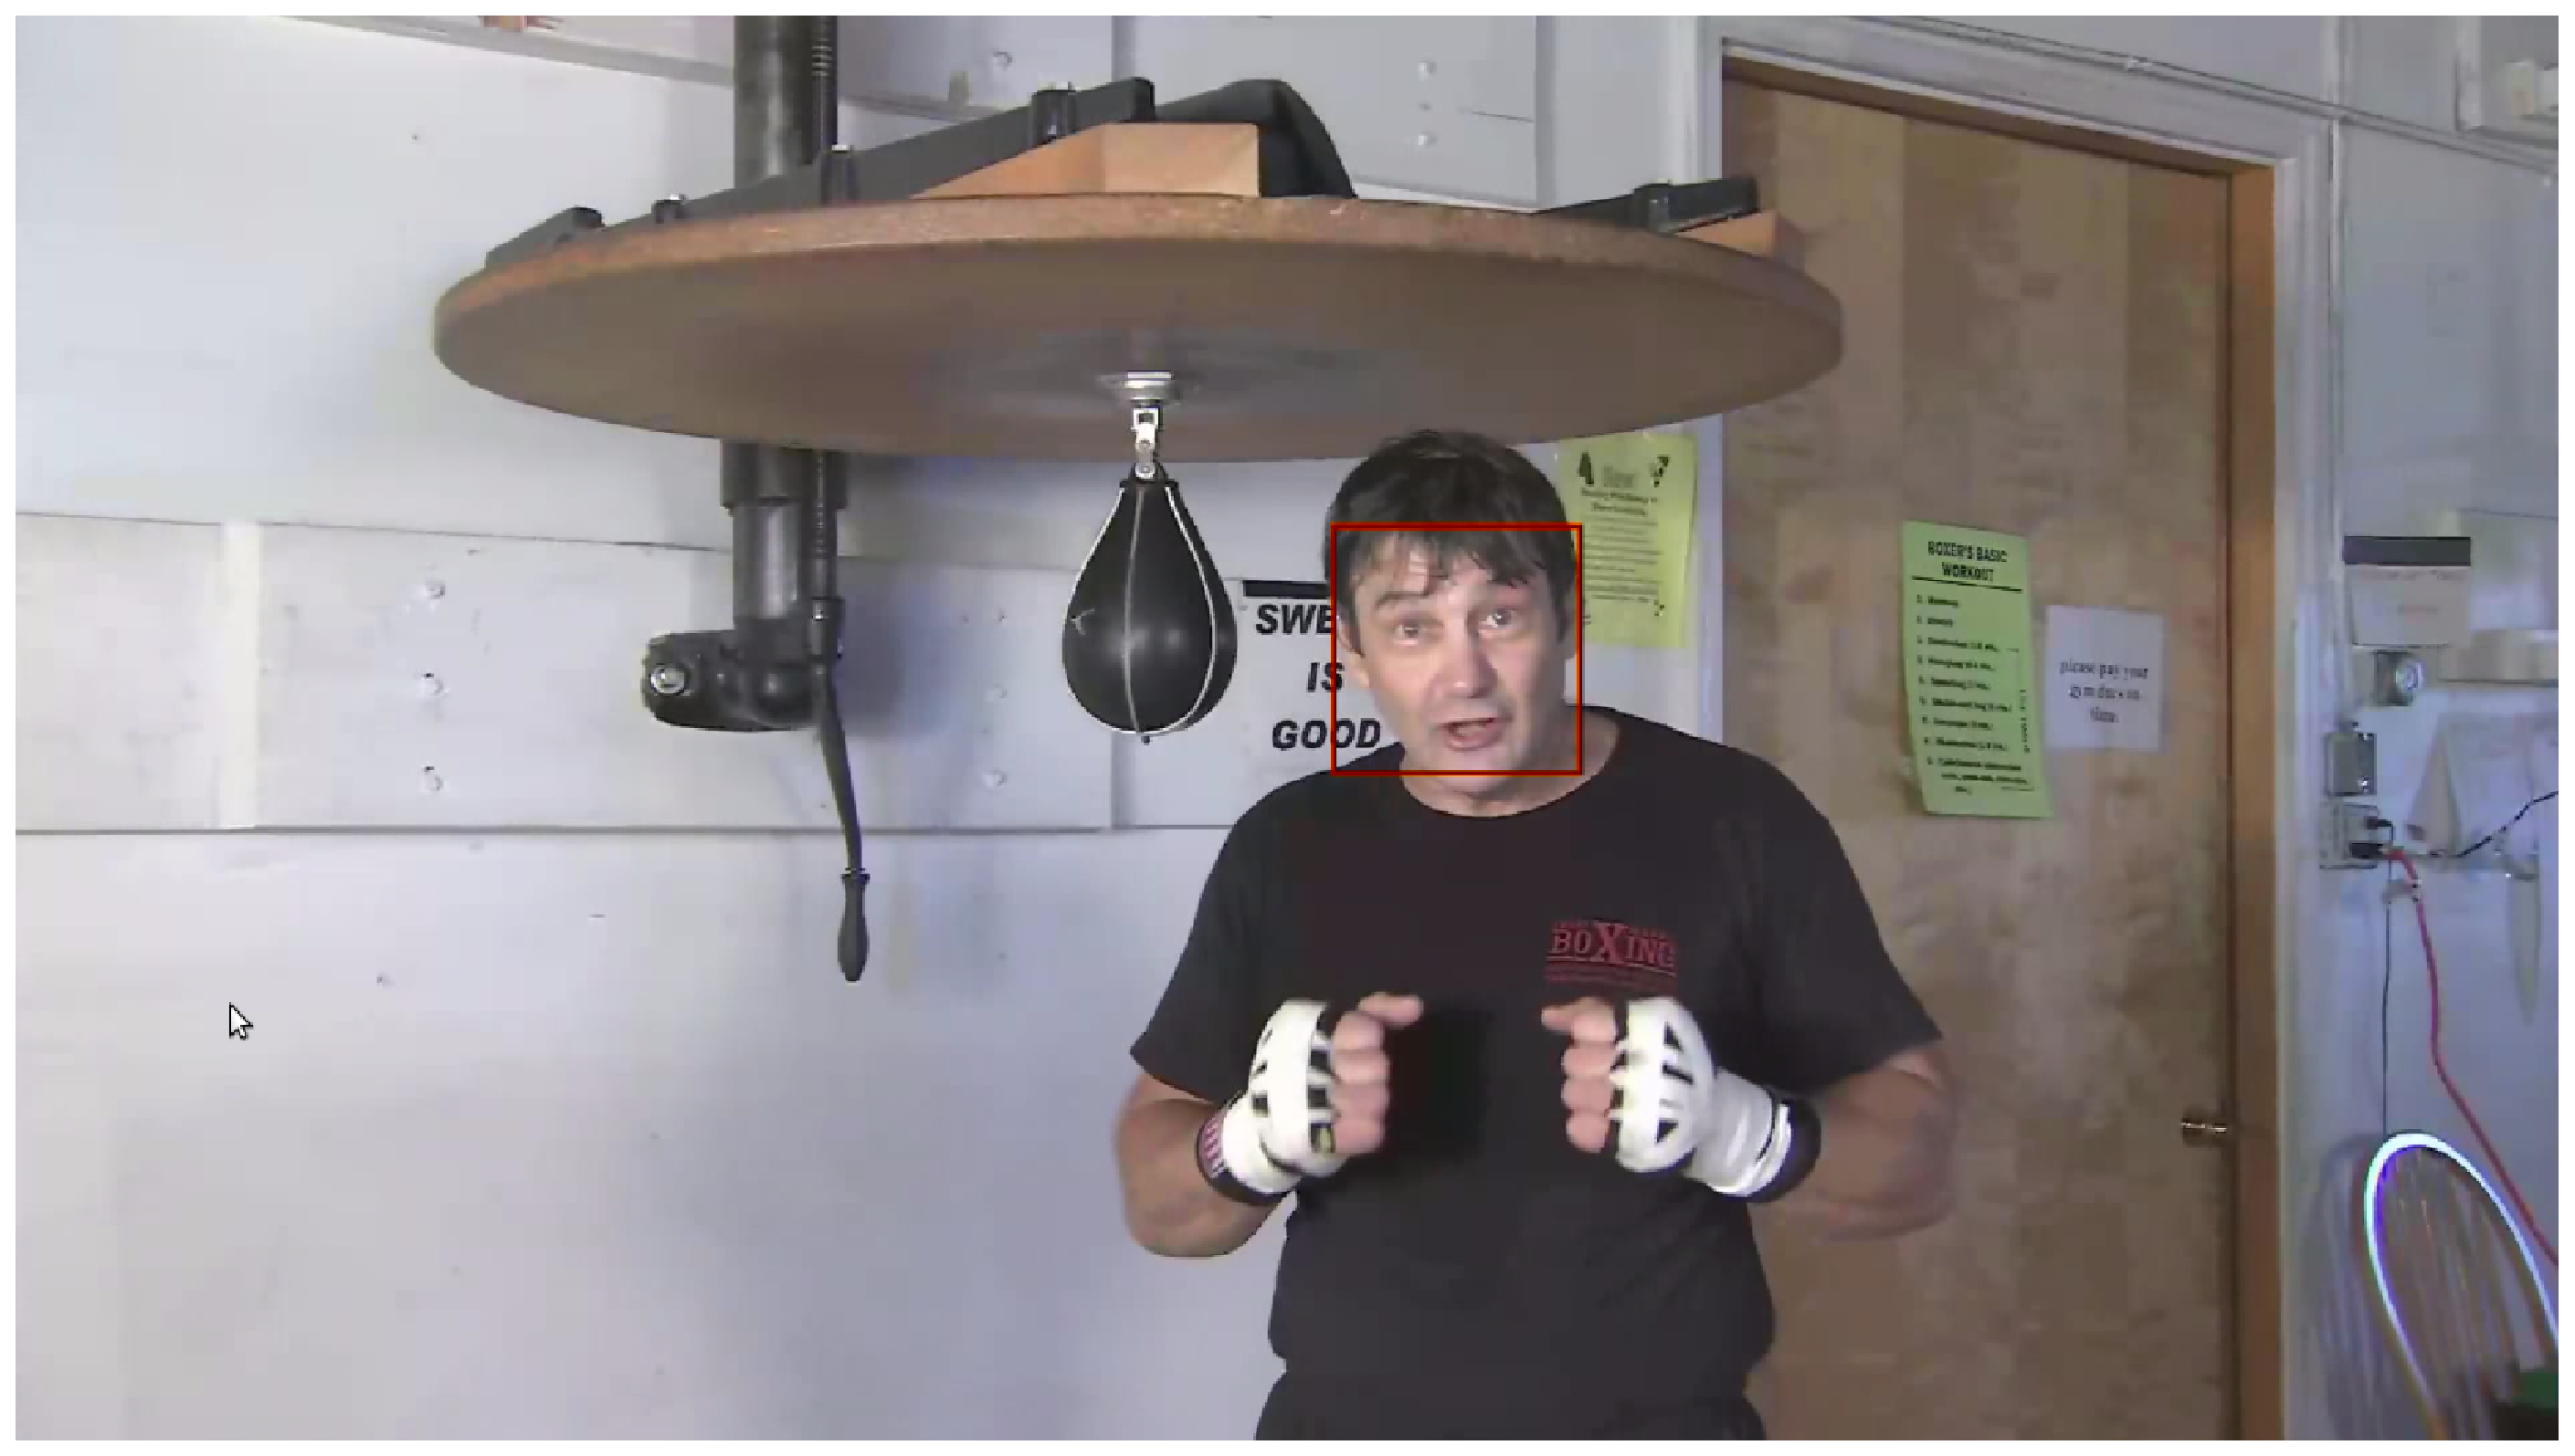
\includegraphics[scale=0.3]{imagens/fig26.eps}
\caption{Face detectada no vídeo \textit{Speed bag}.}
\label{fig:speed_bag_example}
\end{figure}

Utilizando a detecção de objetos em todos os quadros ocorrem diversos falsos positivos, a maior parte dos momentos em que existe a face de perfil ocorrem falsos positivos ou falsos negativos. O momento em que ocorre a face frontal no vídeo possui uma maior quantidade de positivos, porém em alguns momentos ocorrem falsos positivos (um objeto no fundo é detectado como a face), mostrando claramente a limitação que existe ao se configurar o classificador Haar para realizar a detecção de apenas um objeto na imagem. O \textit{tracking} pode se confundir ao detectar outro objeto que não é uma face, já que apenas o primeiro objeto a ser encontrado na imagem é retornado pelo classificador Haar. 

A utilização de histereses ofereceu pouca melhora na qualidade do \textit{tracking}, já que neste vídeo a quantidade de falsos positivos foi muito grande. Apenas no momento em que ocorria a face frontal a histerese mostrou uma melhora significativa, já que a face frontal era detectada e durante a histerese de \textit{tracking} apenas os vetores de movimento calculados pela estimativa de movimento era utilizados para realizar o \textit{tracking}, reduzindo os falsos positivos gerados pelo classificador Haar.

Quanto ao desempenho a ativação de detecção de objetos em todos os quadros tornou o processo de codificação 7,62\% mais lento. A utilização do classificador Haar em conjunto com a estimativa de movimento diminui consideravelmente o custo computacional, com um atraso no processo de codificação variando entre 1,16\% e 0,36\% em relação ao processo de codificação original. O bitstream com os metadados inseridos no pior caso ficou 0,25\% maior que o bitstream original.


Em todos as configurações a qualidade do vídeo codificado mostrou ser a mesma:

\begin{lstlisting}
Y { PSNR (dB), cSNR (dB), MSE }   : {  39.554,  39.283,   7.67013 }
U { PSNR (dB), cSNR (dB), MSE }   : {  43.495,  43.394,   2.97618 }
V { PSNR (dB), cSNR (dB), MSE }   : {  44.830,  44.669,   2.21926 }

Total bits                        : 67278720 (I 9809312, P 57469224, NVB 184) 
Bit rate (kbit/s)  @ 30.00 Hz     : 3540.99
Bits to avoid Startcode Emulation : 0 
Bits for parameter sets           : 184 
Bits for filler data              : 0
\end{lstlisting}


\subsection{ Testes com resolução 720p (1280 x 720) }


Neste teste a resolução do vídeo que foi reduzida de \textit{1080p} (1920 x 1080) para \textit{720p} (1280 x 720), visando a constatação da diferença do impacto do sistema de \textit{tracking} ao processar o mesmo vídeo a resoluções diferentes. O escalonamento do vídeo foi realizado utilizando o Gstreamer.


Especificações do vídeo:

\begin{itemize}
        \item quadros por segundo = 29.97.
        \item total de quadros    = 570.
        \item comprimento         = 1280 pixels.
        \item altura              = 720 pixels.
        \item espaço de cor       = YUV, 4:2:0.
\end{itemize}


\begin{table}[H]
\begin{center}
\begin{tabular}{|p{2.3cm}|p{2.3cm}|p{2.3cm}|p{2.3cm}|p{2.3cm}|p{2.3cm}|}
\hline
\textbf{} & \textbf{\textit{Tracking} Desabilitado} & \textbf{\textit{Tracking} habilitado, sem histerese} & \textbf{Histerese de busca = 5, \textit{tracking} = 10} & \textbf{Histerese de busca = 10, \textit{tracking} = 30} & \textbf{Histerese de busca = 10, \textit{tracking} = 60} \\
\hline
Tempo Total de Codificação (segundos) & 5346.245 & 5843.674 & 5394.242 & 5365.767 & 5352.772 \\
\hline
Tamanho bitstream (bytes) & 4595164 & 4607265 & 4609359 & 4612805 & 4616437 \\
\hline
Atraso no tempo total codificação & 0\% & 9,3\% & 0,89\% & 0,36\% & 0,12\% \\
\hline
Aumento bitstream  & 0\% & 0,26\% & 0,30\% & 0,38\% & 0,46\% \\
\hline
\end{tabular}
\caption{Desempenho do sistema com o vídeo \textit{Speed bag - 720p}.}
\label{tab:space_overhead}
\end{center}
\end{table}


A diminuição da resolução do vídeo não gerou nenhuma diferença na qualidade do \textit{tracking}, porém foi possível perceber um aumento no atraso no tempo total de codificação em todas as configurações. Com \textit{tracking} habilitado e sem histerese, o atraso no vídeo original (\textit{1080p}) foi de 7,62\% enquanto que o atraso gerado no mesmo vídeo, reescalonado para \textit{720p}, foi de 9,3\%, mostrando que a medida que o tamanho do vídeo aumenta o atraso gerado pelo classificador Haar tende a diminuir.


Em todos as configurações a qualidade do vídeo codificado mostrou ser a mesma:

\begin{lstlisting}
Y { PSNR (dB), cSNR (dB), MSE }   : {  39.131,  38.752,   8.66746 }
U { PSNR (dB), cSNR (dB), MSE }   : {  43.023,  42.893,   3.34007 }
V { PSNR (dB), cSNR (dB), MSE }   : {  44.422,  44.220,   2.46079 }

Total bits                        : 36761312 (I 5554416, P 31206720, NVB 176) 
Bit rate (kbit/s)  @ 30.00 Hz     : 1934.81
Bits to avoid Startcode Emulation : 0 
Bits for parameter sets           : 176 
Bits for filler data              : 0
\end{lstlisting}


\section{ Conclusão da avaliação do sistema }


De acordo com os testes realizados a utilização de uma histerese na execução do classificador Haar tornou o sistema mais eficiente. Se somente fosse utilizada a histerese, isso geraria saltos na caixa delimitadora, o uso da estimativa de movimento suavizou esse efeito sem aumentar a complexidade do codificador, já que a estimativa de movimento faz parte do processo normal de codificação. Dependendo da natureza do movimento realizado pelo objeto, a utilização da estimativa de movimento pode gerar resultados inferiores ou superiores á execução do classificador Haar em todos os quadros.

Por exemplo, nos testes apresentados o objeto de interesse era face frontal. Sem utilizar a estimativa de movimento quando uma face se vira de lado o classificador Haar não consegue mais detectar a face que está de perfil, porém utilizando estimativa de movimento o tracking da face de perfil funciona já que uma vez identificado o objeto só é necessário acompanhar seus movimentos. Ao mesmo tempo, dependendo do quanto o objeto de interesse se mover a caixa delimitadora não acompanha perfeitamente o movimento do objeto utilizando as informações de estimativa de movimento. 

Em vídeos com longos trechos sem nenhum objeto de interesse o impacto do classificador Haar tende a ser um pouco menor que o normal, mas em conjunto com a histerese de busca o custo computacional foi reduzido. Inserir um metadado por quadro, mesmo onde o vídeo possui o objeto de interesse em grande parte dos seus quadros, não gerou um bitstream muito maior que o normal, o pior caso não passou de um aumento de 4\%, considerando que quanto maior for a resolução do vídeo e a qualidade do processo de codificação, menor será esse aumento em relação ao bitstream original (isso pode ser observado nos testes com diferentes resoluções).

Com relação ao impacto da utilização do classificador Haar integrado ao codificador em diferentes resoluções, foi possível observar que a medida que a resolução do vídeo aumenta, o custo computacional do processo de codificação tende a aumentar mais que o custo computacional do classificador Haar, já que nos testes em vídeos com alta resolução o impacto da utilização do sistema de \textit{tracking} foi menor que nos vídeos com resoluções menores. Esse resultado foi obtido com o perfil de codificação utilizado nos testes, seria interessante realizar testes com outros perfis de codificação, pois poderiam mostrar resultados diferentes.

Percebe-se também a necessidade de realizar a detecção e \textit{tracking} de múltiplos objetos (que sejam do mesmo padrão, ou seja, utilizem o mesmo arquivo de treinamento para realizar a busca) simultaneamente, como pode ser constatado em \cite{learningOpenCV} página 507, o classificador Haar tende a ter uma baixa taxa de falsos negativos (ou seja, não detectar a presença de um objeto de interesse), em troca de ter uma alta taxa de falsos positivos (detectar um objeto que não é o de interesse), por causa disso utilizar o classificador Haar para retornar o primeiro objeto encontrado simplifica o sistema mas deixa o \textit{tracking} mais suscetível a erros.
  

\chapter{ Conclusões }

Para desenvolver o projeto foi escolhido o software de referência para o padrão de compressão de vídeo MPEG 4 parte 10. Dois tipos de metadados foram desenvolvidos ao longo do trabalho, um representa a caixa delimitadora de um objeto de interesse, o outro é o plano luma bruto de um objeto de interesse. 

Testes realizados tanto com o decodificador de referência como com o Gstreamer mostraram que o uso de mensagens \textit{Supplemental Enhancement Information} do tipo \textit{Unregistered Userdata} para transportar os metadados diretamente no \textit{bitstream} do vídeo não alteraram a conformidade do mesmo com o padrão, sendo possível exibir um vídeo com metadados embutidos em qualquer decodificador MPEG 4 parte 10. 

Apesar do padrão MPEG 4 parte 10 não definir um tamanho máximo para mensagens \textit{Supplemental Enhancement Information} do tipo \textit{Unregistered Userdata}, pode existir um limite implícito no tamanho máximo de um NALU (de acordo com o nível/perfil implementado), o que refletiria em um tamanho máximo para as mensagens. 

Para facilitar a detecção de objetos foi utilizado um algoritmo de detecção de padrões em imagens estáticas, o classificador Haar, implementado na biblioteca de visão computacional OpenCV. Executar o classificador Haar em todos os quadros do vídeo mostrou um aumento considerável no custo computacional do codificador. 

Utilizou-se informações de estimativa de movimento calculadas pelo codificador para estimar o movimento do objeto, evitando a necessidade de executar o classificador Haar em todos os quadros do vídeo, dessa maneira constatou-se uma significativa redução do custo computacional reutilizando informações geradas pelo processo de codificação. Com as alterações realizadas no decodificador de referência foi possível recuperar os metadados. Os metadados representando a caixa delimitadora de um objeto detectado, são desenhados no quadro, facilitando a constatação visual do funcionamento do sistema.  

Como toda a extração do metadado e inserção dele dentro do \textit{bitstream} é feita internamente no codificador isso facilita a construção de um chip codificador H.264 que realize \textit{tracking} de objetos, esse chip codificador poderia ter grande parte do classificador Haar acelerado também em hardware, dentro do chip. Como pode ser visto em \cite{haarFPGA}, obtêm-se um grande aumento no desempenho da detecção de objetos ao se implementar o classificador Haar em FPGA. 

Este trabalhou mostrou a viabilidade de se utilizar a estimativa de movimento gerada pelo codificador para auxiliar o \textit{tracking} de objetos e do envio dessas informações através do \textit{bitstream} do vídeo. Além das informações de \textit{tracking} foi possível enviar o objeto detectado não compactado como metadado, o que pode ser útil em algoritmos de identificação biométrica. No momento da análise dos vídeos é necessário analisar apenas os metadados que estão inseridos no \textit{bitstream}, grande parte do processamento já foi realizado durante o processo de codificação. 


\section{Trabalhos futuros}

Como possíveis trabalhos futuros, cita-se: 

\begin{itemize}
        \item Fazer um melhor uso das informações geradas pelo processo de codificação para gerar heurísticas mais inteligentes. Um exemplo seria utilizar histereses dinâmicas, quando existe muito movimento no vídeo as histereses diminuem, mas quando não existe movimento as histereses aumentam.
        \item Estender o sistema para realizar a detecção e \textit{tracking} de múltiplos objetos (com mesma forma) simultaneamente.
        \item Buscar no classificador Haar cálculos que já possam ter sido feitos pelo codificador, melhorando a integração dos dois.
        \item Utilizar outro algoritmo de detecção de padrões que tenha uma maior interseção com os algoritmos presentes no codificador.
        \item Utilizar apenas as informações de estimativa de movimento para a construção de cercas virtuais ou alarmes que não se importem com a forma do objeto mas com padrões de movimento suspeitos.
        \item Desenvolver um chip codificador H.264 integrado ao classificador Haar integrado no chip, realizando a detecção e \textit{tracking} de objetos em tempo real. Cita-se \cite{haarFPGA} como exemplo de um classificador Haar acelerado em hardware.
\end{itemize}
  


\bibliography{ref}

\chapter{APÊNDICE A -- CODIGO FONTE DO PROCEDIMENTO DE TESTE DA INSERÇÃO DE NALUs SEI}

No caso dos módulos novos, todo o seu fonte é documentado aqui.

No caso dos módulos que já existiam no software de referência e sofreram alterações, apenas as funções que sofreram alteração serão documentadas aqui.


\section{Módulo adicionado ao Codificador}

\subsection{Arquivo udata\_gen.h}

\begin{lstlisting}
/*!
 *******************************************************************************
 *  \file
 *     udata_gen.h
 *  \brief
 *     definitions for Supplemental Enhanced Information Userdata Generation
 *  \author(s)
 *      - Tiago Katcipis                             <tiagokatcipis@gmail.com>
 *
 * *****************************************************************************
 */

#ifndef UDATA_GEN_H
#define UDATA_GEN_H

#include "typedefs.h"
#include "nal.h"

/*!
 *****************************************************************************************
 * Generates a SEI NALU that with ONE unregistered userdata SEI message.
 *
 * @param data The data to be sent on the SEI unregistered userdata message.
 * @param size The size of the data.
 * @return A SEI NALU containing the SEI message.
 *
 *****************************************************************************************
 */
NALU_t *user_data_generate_unregistered_sei_nalu(char * data, unsigned int size);

/*!
 *****************************************************************************************
 * Generates a SEI NALU that with ONE unregistered userdata SEI message.
 *
 * @param msg The message to be sent on the SEI unregistered userdata message, 
 *            must be a 0 terminated string.
 * @return A SEI NALU containing the SEI message.
 *
 ******************************************************************************************
 */
NALU_t *user_data_generate_unregistered_sei_nalu_from_msg(char * msg);

/*!
 *******************************************************************************************
 * Generates a 0 terminated string to be sent on a SEI NALU. The size of the message is
 * random, but it will not exceed MAXNALUSIZE.
 *
 * @return a 0 terminated string.
 *
 ********************************************************************************************
 */
char* user_data_generate_create_random_message();

/*!
 *******************************************************************************************
 * Frees the resources used by a msg.
 *
 * @param msg A previously created message.
 *
 ********************************************************************************************
 */
void user_data_generate_destroy_random_message(char * msg);

#endif
\end{lstlisting}

\subsection{Arquivo udata\_gen.c}
\begin{lstlisting}

#include <string.h>
#include <stdio.h>
#include <stdlib.h>
#include "udata_gen.h"
#include "vlc.h"
#include "sei.h"
#include "nalu.h"


static const char* random_message_start_template = "\nRandom message[%d] start\n";
static const char* random_message_end_template   = "\nRandom message[%d] end!\n";
static int msg_counter                           = 1;

/* Lets guarantee that max_msg_size + headers + 
   emulation prevention bytes dont exceed the MAXNALUSIZE */
static const int max_msg_size                    = MAXNALUSIZE - 1024; 

static int growth_rate                           = 1024;
static int actual_size                           = 1024;

#define MAX_TEMPLATE_MSG_SIZE 512
static char random_message_start_buffer[MAX_TEMPLATE_MSG_SIZE];
static char random_message_end_buffer[MAX_TEMPLATE_MSG_SIZE]; 

/*!
 *************************************************************************************
 * \brief
 *    int GenerateUserDataSEImessage_rbsp(int, byte*, char*, unsigned int)
 *
 * \return
 *    size of the RBSP in bytes, negative in case of an error
 *
 *************************************************************************************
 */
static int GenerateUserDataSEImessage_rbsp (int id, byte *rbsp, char* sei_message, unsigned int sei_message_size)
{
  Bitstream *bitstream;
  unsigned int message_size = sei_message_size;

  int LenInBytes;
  assert (rbsp != NULL);

  if ((bitstream=calloc(1, sizeof(Bitstream)))==NULL)
    no_mem_exit("SeqParameterSet:bitstream");

  // .. and use the rbsp provided (or allocated above) for the data
  bitstream->streamBuffer = rbsp;
  bitstream->bits_to_go = 8;

  {
    char uuid_message[9] = "Random"; // This is supposed to be Random
    unsigned int i;

    TIME_T start_time;
    gettime(&start_time);    // start time

    u_v (8,"SEI: last_payload_type_byte", 5, bitstream);
    message_size += 17;
    while (message_size > 254)
    {
      u_v (8,"SEI: ff_byte",255, bitstream);
      message_size -= 255;
    }
    u_v (8,"SEI: last_payload_size_byte",message_size, bitstream);

    // Lets randomize uuid based on time
    u_v (32,"SEI: uuid_iso_iec_11578",(int) start_time.tv_sec, bitstream);
    u_v (32,"SEI: uuid_iso_iec_11578",(int) start_time.tv_usec, bitstream);

    u_v (32,"SEI: uuid_iso_iec_11578",(int) (uuid_message[0] << 24) + (uuid_message[1] << 16)  + (uuid_message[2] << 8) + (uuid_message[3] << 0), bitstream);
    u_v (32,"SEI: uuid_iso_iec_11578",(int) (uuid_message[4] << 24) + (uuid_message[5] << 16)  + (uuid_message[6] << 8) + (uuid_message[7] << 0), bitstream);

    for (i = 0; i < sei_message_size; i++) {
        u_v (8,"SEI: user_data_payload_byte",sei_message[i], bitstream);
    }

    /* FIXME we MUST have this zero or the original coded was suposed to zero terminate the msg ? */
    u_v (8,"SEI: user_data_payload_byte", 0, bitstream);
  }

  SODBtoRBSP(bitstream);     // copies the last couple of bits into the byte buffer
  LenInBytes=bitstream->byte_pos;

  free(bitstream);
  return LenInBytes;
}


/*!
 *************************************************************************************
 * \brief
 *    Function body for Unregistered userdata SEI message NALU generation
 *
 * \return
 *    A NALU containing the SEI message.
 *
 *************************************************************************************
 */
NALU_t * user_data_generate_unregistered_sei_nalu(char * data, unsigned int size)
{
  NALU_t *n = AllocNALU(MAXNALUSIZE);
  int RBSPlen = 0;
  byte rbsp[MAXRBSPSIZE];

  RBSPlen = GenerateUserDataSEImessage_rbsp (NORMAL_SEI, rbsp, data, size);
  RBSPtoNALU (rbsp, n, RBSPlen, NALU_TYPE_SEI, NALU_PRIORITY_DISPOSABLE, 1);

  n->startcodeprefix_len = 4;
  return n;
}


/*!
 *************************************************************************************
 * \brief
 *    Function body for Unregistered userdata SEI message NALU generation
 *
 * \return
 *    A NALU containing the SEI message.
 *
 *************************************************************************************
 */
NALU_t *user_data_generate_unregistered_sei_nalu_from_msg(char * msg)
{
    return user_data_generate_unregistered_sei_nalu(msg, strlen(msg));
}


/*!
 *************************************************************************************
 * \brief
 *    Function body for random string message generation.
 *
 * \return
 *    A 0 terminted string.
 *
 *************************************************************************************
 */
char* user_data_generate_create_random_message()
{
    char * msg    = 0;
    int msg_size  = 0;
    int body_size = 0;
    int start_len = 0;
    int end_len   = 0;
    int i         = 0;

    /* This will help debug of the SEI messages at the decoder */
    snprintf (random_message_start_buffer, MAX_TEMPLATE_MSG_SIZE, random_message_start_template, msg_counter);
    snprintf (random_message_end_buffer, MAX_TEMPLATE_MSG_SIZE, random_message_end_template, msg_counter);
    msg_counter++;

    start_len = strlen(random_message_start_buffer);
    end_len  = strlen(random_message_end_buffer);

    body_size = actual_size;
    actual_size += growth_rate;

    if (actual_size > max_msg_size) {
        actual_size = growth_rate;
    }
    
    msg_size = body_size + start_len +  end_len + 1;
    msg      = malloc(msg_size);

    /* writing the start */
    memcpy(msg, random_message_start_buffer, start_len);
    
    /* writing the body */
    for (i = start_len; i < msg_size - end_len; i++) {
        msg[i] = 'h'; /* whatever */
    }

    /* writing the end */
    memcpy(msg + start_len + body_size, random_message_end_buffer, end_len);

    /* 0 terminate it */
    msg[msg_size - 1] = '\0';
    return msg;
}

/*!
 *************************************************************************************
 * \brief
 *    Function body for random message destruction.
 *************************************************************************************
 */
void user_data_generate_destroy_random_message(char * msg)
{
    free(msg);
}
\end{lstlisting}

\section{Alterações no Codificador}

\subsection{Arquivo filehandle.c}
\begin{lstlisting}

/*!
 ************************************************************************
 * \brief
 *    This function opens the output files and generates the
 *    appropriate sequence header
 ************************************************************************
 */
int start_sequence(VideoParameters *p_Vid, InputParameters *p_Inp)
{
  int i,len=0, total_pps = (p_Inp->GenerateMultiplePPS) ? 3 : 1;
  NALU_t *nalu;

  switch(p_Inp->of_mode)
  {
    case PAR_OF_ANNEXB:
      OpenAnnexbFile (p_Vid, p_Inp->outfile);
      p_Vid->WriteNALU = WriteAnnexbNALU;
      break;
    case PAR_OF_RTP:
      OpenRTPFile (p_Vid, p_Inp->outfile);
      p_Vid->WriteNALU = WriteRTPNALU;
      break;
    default:
      snprintf(errortext, ET_SIZE, "Output File Mode %d not supported", p_Inp->of_mode);
      error(errortext,1);
  }

  // Access Unit Delimiter NALU
  if ( p_Inp->SendAUD )
  {
    len += Write_AUD_NALU(p_Vid);
  }

  //! As a sequence header, here we write both sequence and picture
  //! parameter sets.  As soon as IDR is implemented, this should go to the
  //! IDR part, as both parsets have to be transmitted as part of an IDR.
  //! An alternative may be to consider this function the IDR start function.

  nalu = NULL;
  nalu = GenerateSeq_parameter_set_NALU (p_Vid);
  len += p_Vid->WriteNALU (p_Vid, nalu);
  FreeNALU (nalu);

#if (MVC_EXTENSION_ENABLE)
  if(p_Inp->num_of_views==2)
  {
    int bits;
    nalu = NULL;
    nalu = GenerateSubsetSeq_parameter_set_NALU (p_Vid);
    bits = p_Vid->WriteNALU (p_Vid, nalu);
    len += bits;
    p_Vid->p_Stats->bit_ctr_parametersets_n_v[1] = bits;
    FreeNALU (nalu);
  }
  else
  {
    p_Vid->p_Stats->bit_ctr_parametersets_n_v[1] = 0;
  }
#endif

  //! Lets write now the Picture Parameter sets. Output will be equal to the total number of bits spend here.
  for (i=0;i<total_pps;i++)
  {
     len = write_PPS(p_Vid, len, i);
  }

  if (p_Inp->GenerateSEIMessage)
  {
    nalu = NULL;
    nalu = GenerateSEImessage_NALU(p_Inp);
    len += p_Vid->WriteNALU (p_Vid, nalu);
    FreeNALU (nalu);
  }

  /* Lets send 1000 SEI NALUs containing a SEI Userdata Unregistered message */
  for (i = 0; i < 1000; i++) {
      nalu = NULL;
      char * msg = user_data_generate_create_random_message();
      nalu = user_data_generate_unregistered_sei_nalu_from_msg(msg);
      len += p_Vid->WriteNALU (p_Vid, nalu);
      FreeNALU (nalu);
      user_data_generate_destroy_random_message(msg);
  }


  p_Vid->p_Stats->bit_ctr_parametersets_n = len;
#if (MVC_EXTENSION_ENABLE)
  if(p_Inp->num_of_views==2)
  {
    p_Vid->p_Stats->bit_ctr_parametersets_n_v[0] = len - p_Vid->p_Stats->bit_ctr_parametersets_n_v[1];
  }
#endif
  return 0;
}
\end{lstlisting}

\subsection{Arquivo lencod.c}
\begin{lstlisting}
/*!
 ***********************************************************************
 * \brief
 *    Encode a sequence
 ***********************************************************************
 */
static void encode_sequence(VideoParameters *p_Vid, InputParameters *p_Inp)
{
  int curr_frame_to_code;
  int frames_to_code;
  int frame_num_bak = 0, frame_coded;
  int frm_struct_buffer;
  SeqStructure *p_seq_struct = p_Vid->p_pred;
  FrameUnitStruct *p_frm;

#if (MVC_EXTENSION_ENABLE)
  int tmp_rate_control_enable = p_Inp->RCEnable;

  if ( p_Inp->num_of_views == 2 )
  {
    frames_to_code = p_Inp->no_frames << 1;
    p_frm = p_seq_struct->p_frm_mvc;
    frm_struct_buffer = p_seq_struct->num_frames_mvc;
  }
  else
#endif
  {
    frames_to_code = p_Inp->no_frames;
    p_frm = p_seq_struct->p_frm;
    frm_struct_buffer = p_Vid->frm_struct_buffer;
  }
  
  for (curr_frame_to_code = 0; curr_frame_to_code < frames_to_code; curr_frame_to_code++)
  {
#if (MVC_EXTENSION_ENABLE)
    if ( p_Inp->num_of_views == 2 )
    {
      if ( (curr_frame_to_code & 1) == 0 ) // call only for view_id 0
      {
        // determine whether to populate additional frames in the prediction structure
        if ( (curr_frame_to_code >> 1) >= p_Vid->p_pred->pop_start_frame )
        {
          int start = p_seq_struct->pop_start_frame, end;

          populate_frm_struct( p_Vid, p_Inp, p_seq_struct, p_Inp->FrmStructBufferLength, frames_to_code >> 1 );
          end = p_seq_struct->pop_start_frame;
          populate_frm_struct_mvc( p_Vid, p_Inp, p_seq_struct, start, end );
        }
      }
    }
    else
#endif
    {
      // determine whether to populate additional frames in the prediction structure
      if ( curr_frame_to_code >= p_Vid->p_pred->pop_start_frame )
      {
        populate_frm_struct( p_Vid, p_Inp, p_seq_struct, p_Inp->FrmStructBufferLength, frames_to_code );
      }
    }

    p_Vid->curr_frm_idx = curr_frame_to_code;
    p_Vid->p_curr_frm_struct = p_frm + ( p_Vid->curr_frm_idx % frm_struct_buffer ); // pointer to current frame structure
    p_Vid->number = curr_frame_to_code;

#if (MVC_EXTENSION_ENABLE)
    if(p_Inp->num_of_views==2)
    {
      p_Vid->view_id = p_Vid->p_curr_frm_struct->view_id;
      if ( p_Vid->view_id == 1 )
      {
        p_Vid->curr_frm_idx = p_Vid->number = (curr_frame_to_code - 1) >> 1;
        p_Vid->p_curr_frm_struct->qp = p_Vid->qp = iClip3( -p_Vid->bitdepth_luma_qp_scale, MAX_QP, p_Vid->AverageFrameQP + p_Inp->View1QPOffset );
      }
      else
      {
        p_Vid->curr_frm_idx = p_Vid->number = curr_frame_to_code >> 1;
      }
      if ( p_Vid->view_id == 1 && tmp_rate_control_enable )
      {
        p_Inp->RCEnable = 0;        
      }
      else
      {
        p_Inp->RCEnable = tmp_rate_control_enable;
      }
    }
#endif

    if ( p_Vid->p_curr_frm_struct->frame_no >= p_Inp->no_frames )
    {
      continue;
    }

    // Update frame_num counter
    frame_num_bak = p_Vid->frame_num;
    if (p_Vid->last_ref_idc == 1)
    {      
      p_Vid->frame_num++;

#if (MVC_EXTENSION_ENABLE)
      if ( p_Inp->num_of_views == 2 )
      {
        p_Vid->frame_num %= (p_Vid->max_frame_num << 1);
      }
      else
#endif
      p_Vid->frame_num %= p_Vid->max_frame_num;
    }

    prepare_frame_params(p_Vid, p_Inp, curr_frame_to_code);

    // redundant frame initialization and allocation
    if (p_Inp->redundant_pic_flag)
    {
      init_redundant_frame(p_Vid, p_Inp);
      set_redundant_frame(p_Vid, p_Inp);
    }

    frame_coded = encode_one_frame(p_Vid, p_Inp); // encode one frame;
    if ( !frame_coded )
    {
      p_Vid->frame_num = frame_num_bak;
      continue;
    }

    p_Vid->last_ref_idc = p_Vid->nal_reference_idc ? 1 : 0;

    // if key frame is encoded, encode one redundant frame
    if (p_Inp->redundant_pic_flag && p_Vid->key_frame)
    {
      encode_one_redundant_frame(p_Vid, p_Inp);
    }

    if (p_Vid->type == I_SLICE && p_Inp->EnableOpenGOP)
      p_Vid->last_valid_reference = p_Vid->ThisPOC;

    if (p_Inp->ReportFrameStats)
      report_frame_statistic(p_Vid, p_Inp);

    /* Inserting a SEI NALU (Userdata Unregistered) */
    char * msg   = user_data_generate_create_random_message();
    NALU_t *nalu = user_data_generate_unregistered_sei_nalu_from_msg(msg);
    p_Vid->WriteNALU (p_Vid, nalu);
    FreeNALU (nalu);
    user_data_generate_destroy_random_message(msg);
  }

#if EOS_OUTPUT
  end_of_stream(p_Vid);
#endif

#if (MVC_EXTENSION_ENABLE)
  if(p_Inp->num_of_views == 2)
  {
    p_Inp->RCEnable = tmp_rate_control_enable;
  }
#endif
}
\end{lstlisting}

\section{Módulo adicionado ao Decodificador}

\subsection{Arquivo udata\_parser.h}
\begin{lstlisting}
/*!
 ************************************************************************
 *  \file
 *     udata_parser.h
 *  \brief
 *     definitions for Supplemental Enhanced Information Userdata Parsing
 *  \author(s)
 *      - Tiago Katcipis                             <tiagokatcipis@gmail.com>
 *
 * ************************************************************************
 */

#ifndef UDATA_PARSER_H
#define UDATA_PARSER_H

#include "typedefs.h"

/*!
 *******************************************************************************
 * Parses a SEI User Data Unregistered message, dumping all its data at stdout.
 *
 * @param payload The payload of the SEI message.
 * @param size The size of the payload.
 *
 *******************************************************************************
 */
void user_data_parser_unregistered_sei(byte* payload, int size);

#endif
\end{lstlisting}

\subsection{Arquivo udata\_parser.c}
\begin{lstlisting}
#include "udata_parser.h"
#include <stdio.h>

#define UUID_ISO_IEC_OFFSET 16 


void user_data_parser_unregistered_sei( byte* payload, int size)
{
  int offset = 0;
  byte payload_byte;

  printf("\nUser data unregistered SEI message, size[%d]\n", size);
  printf("uuid_iso_11578 = 0x");
  
  assert (size>=UUID_ISO_IEC_OFFSET);

  for (offset = 0; offset < UUID_ISO_IEC_OFFSET; offset++)
  {
    printf("%02x",payload[offset]);
  }

  printf("\nUser data unregistered SEI message start\n");

  while (offset < size)
  {
    payload_byte = payload[offset];
    offset ++;
    printf("%c", payload_byte);
  }

  printf("\nUser data unregistered SEI message end \n");
}
\end{lstlisting}

\section{Alterações no Decodificador}

\subsection{Arquivo sei.c}
\begin{lstlisting}
void InterpretSEIMessage(byte* msg, int size, VideoParameters *p_Vid, Slice *pSlice)
{
  int payload_type = 0;
  int payload_size = 0;
  int offset = 1;
  byte tmp_byte;
  
  do
  {
    // sei_message();
    payload_type = 0;
    tmp_byte = msg[offset++];
    while (tmp_byte == 0xFF)
    {
      payload_type += 255;
      tmp_byte = msg[offset++];
    }
    payload_type += tmp_byte;   // this is the last byte

    payload_size = 0;
    tmp_byte = msg[offset++];
    while (tmp_byte == 0xFF)
    {
      payload_size += 255;
      tmp_byte = msg[offset++];
    }
    payload_size += tmp_byte;   // this is the last byte

    switch ( payload_type )     // sei_payload( type, size );
    {
    case  SEI_BUFFERING_PERIOD:
      interpret_buffering_period_info( msg+offset, payload_size, p_Vid );
      break;
    case  SEI_PIC_TIMING:
      interpret_picture_timing_info( msg+offset, payload_size, p_Vid );
      break;
    case  SEI_PAN_SCAN_RECT:
      interpret_pan_scan_rect_info( msg+offset, payload_size, p_Vid );
      break;
    case  SEI_FILLER_PAYLOAD:
      interpret_filler_payload_info( msg+offset, payload_size, p_Vid );
      break;
    case  SEI_USER_DATA_REGISTERED_ITU_T_T35:
      interpret_user_data_registered_itu_t_t35_info( msg+offset, payload_size, p_Vid );
      break;
    case  SEI_USER_DATA_UNREGISTERED:
      user_data_parser_unregistered_sei(msg+offset, payload_size);
      break;
    case  SEI_RECOVERY_POINT:
      interpret_recovery_point_info( msg+offset, payload_size, p_Vid );
      break;
    case  SEI_DEC_REF_PIC_MARKING_REPETITION:
      interpret_dec_ref_pic_marking_repetition_info( msg+offset, payload_size, p_Vid, pSlice );
      break;
    case  SEI_SPARE_PIC:
      interpret_spare_pic( msg+offset, payload_size, p_Vid );
      break;
    case  SEI_SCENE_INFO:
      interpret_scene_information( msg+offset, payload_size, p_Vid );
      break;
    case  SEI_SUB_SEQ_INFO:
      interpret_subsequence_info( msg+offset, payload_size, p_Vid );
      break;
    case  SEI_SUB_SEQ_LAYER_CHARACTERISTICS:
      interpret_subsequence_layer_characteristics_info( msg+offset, payload_size, p_Vid );
      break;
    case  SEI_SUB_SEQ_CHARACTERISTICS:
      interpret_subsequence_characteristics_info( msg+offset, payload_size, p_Vid );
      break;
    case  SEI_FULL_FRAME_FREEZE:
      interpret_full_frame_freeze_info( msg+offset, payload_size, p_Vid );
      break;
    case  SEI_FULL_FRAME_FREEZE_RELEASE:
      interpret_full_frame_freeze_release_info( msg+offset, payload_size, p_Vid );
      break;
    case  SEI_FULL_FRAME_SNAPSHOT:
      interpret_full_frame_snapshot_info( msg+offset, payload_size, p_Vid );
      break;
    case  SEI_PROGRESSIVE_REFINEMENT_SEGMENT_START:
      interpret_progressive_refinement_start_info( msg+offset, payload_size, p_Vid );
      break;
    case  SEI_PROGRESSIVE_REFINEMENT_SEGMENT_END:
      interpret_progressive_refinement_end_info( msg+offset, payload_size, p_Vid );
      break;
    case  SEI_MOTION_CONSTRAINED_SLICE_GROUP_SET:
      interpret_motion_constrained_slice_group_set_info( msg+offset, payload_size, p_Vid );
    case  SEI_FILM_GRAIN_CHARACTERISTICS:
      interpret_film_grain_characteristics_info ( msg+offset, payload_size, p_Vid );
      break;
    case  SEI_DEBLOCKING_FILTER_DISPLAY_PREFERENCE:
      interpret_deblocking_filter_display_preference_info ( msg+offset, payload_size, p_Vid );
      break;
    case  SEI_STEREO_VIDEO_INFO:
      interpret_stereo_video_info_info ( msg+offset, payload_size, p_Vid );
      break;
    case  SEI_TONE_MAPPING:
      interpret_tone_mapping( msg+offset, payload_size, p_Vid );
      break;
    case  SEI_POST_FILTER_HINTS:
      interpret_post_filter_hints_info ( msg+offset, payload_size, p_Vid );
      break;
    case  SEI_FRAME_PACKING_ARRANGEMENT:
      interpret_frame_packing_arrangement_info( msg+offset, payload_size, p_Vid );
      break;
    default:
      interpret_reserved_info( msg+offset, payload_size, p_Vid );
      break;    
    }
    offset += payload_size;

  } while( msg[offset] != 0x80 );    // more_rbsp_data()  msg[offset] != 0x80
  // ignore the trailing bits rbsp_trailing_bits();
  assert(msg[offset] == 0x80);      // this is the trailing bits
  assert( offset+1 == size );
}

\end{lstlisting}


\chapter{APÊNDICE B -- CÓDIGO FONTE DO MÓDULO EXTRACTED\_METADATA}

\section{extracted\_metadata.h}

\begin{lstlisting}

/*!
 *******************************************************************************
 *  \file
 *     extracted_metadata.h
 *  \brief
 *     definitions for the extracted metadata.
 *  \author(s)
 *      - Tiago Katcipis                             <tiagokatcipis@gmail.com>
 *
 * *****************************************************************************
 */

#ifndef EXTRACTED_METADATA_H
#define EXTRACTED_METADATA_H

typedef struct _ExtractedYImage ExtractedYImage;
typedef struct _ExtractedMetadata ExtractedMetadata;
typedef struct _ExtractedMetadataBuffer ExtractedMetadataBuffer;
typedef struct _ExtractedObjectBoundingBox ExtractedObjectBoundingBox;


/* ExtractedObjectBoundingBox API */

/*!
 *******************************************************************************
 * Creates a new extracted object bounding box.
 *
 * @param id The id of the bounding box object.
 * @param frame_num The frame number this metadata belongs.
 * @param x The x coordinate of the bounding box.
 * @param y The y coordinate of the bounding box.
 * @param width The width of the bounding box.
 * @param height The height of the bounding box.
 * @return The newly allocated ExtractedObjectBoundingBox object.
 *
 *******************************************************************************
 */
ExtractedObjectBoundingBox * extracted_object_bounding_box_new(unsigned int id, 
                                                               unsigned int frame_num, 
                                                               int x, 
                                                               int y, 
                                                               int width, 
                                                               int height);


/*!
 *******************************************************************************
 *  Gets data about an object bouding box, any parameter can be ommited 
 *  (passing NULL) if you are not interested on it.
 *
 * @param box The ExtractedObjectBoundingBox object.
 * @param id The id of the bounding box. (OUT) (Optional)
 * @param x The x coordinate of the bouding box. (OUT) (Optional)
 * @param y The y coordinate of the bounding box. (OUT) (Optional)
 * @param width The width of the bounding box. (OUT) (Optional)
 * @param height The height of the bounding box. (OUT) (Optional)
 *
 *******************************************************************************
 */
void extracted_object_bounding_box_get_data(ExtractedObjectBoundingBox * box, 
                                            unsigned int * id,
                                            int * x,
                                            int * y,
                                            int * width,
                                            int * height);


/*!
 *********************************************************************************
 * If the given metadata is of the type ExtractedObjectBoundingBox,
 * returns the ExtractedObjectBoundingBox object, NULL otherwise.
 *
 * @param metadata The metadata object.
 * @return The ExtractedObjectBoundingBox object or NULL if the type is not right.
 *
 *********************************************************************************
 */
ExtractedObjectBoundingBox * extracted_object_bounding_box_from_metadata(ExtractedMetadata * metadata);


/* ExtractedYImage API */

/*!
 *******************************************************************************
 * Creates a new extracted image, the image only has the luma plane (Y).
 *
 * @param frame_num The frame number this metadata belongs.
 * @param width The width of the image that will be saved.
 * @param height The height of the image that will be saved.
 * @return The newly allocated ExtractedImage object.
 *
 *******************************************************************************
 */
ExtractedYImage * extracted_y_image_new(unsigned int frame_num, int width, int height);


/*!
 *******************************************************************************
 * Get the luma plane of the extracted image.
 * y[row][col] format. Each pixel has 8 bits depth.
 *
 * @return The luma plane.
 *
 *******************************************************************************
 */
unsigned char ** extracted_y_image_get_y(ExtractedYImage * img);


/* ExtractedMetadata API */

/*!
 *******************************************************************************
 * Gets the size in bytes necessary to serialize this ExtractedMetadata object.
 *
 * @param metadata The metadata to get the serialized size in bytes.
 * @return The serialized size (in bytes) of this ExtractedMetadata.
 *
 *******************************************************************************
 */
int extracted_metadata_get_serialized_size(ExtractedMetadata * metadata);

/*!
 *******************************************************************************
 * Serialize this ExtractedMetadata object. It is responsability of the caller
 * to alloc a data pointer with the right size and to free it after usage.
 * The right size can be get with extracted_metadata_get_serialized_size.
 *
 * @param metadata The metadata to serialize.
 * @param serialized_data Where the serialized metadata will be stored.
 *
 *******************************************************************************
 */
void extracted_metadata_serialize(ExtractedMetadata * metadata, char * serialized_data);

/*!
 *******************************************************************************
 * Deserialize this ExtractedMetadata object. 
 *
 * @param data The serialized metadata.
 * @param size Size in bytes of the serialized object.
 * @return The deserialized ExtractedMetadata object or NULL in case of error.
 *
 *******************************************************************************
 */
ExtractedMetadata * extracted_metadata_deserialize(const char * data, int size);

/*!
 *******************************************************************************
 * Save this ExtractedMetadata object on a file. 
 *
 * @param metadata The metadata to be saved.
 * @param fd File descriptor where the metadata will be saved.
 *
 *******************************************************************************
 */
void extracted_metadata_save(ExtractedMetadata * metadata, int fd);

/*!
 *******************************************************************************
 * Frees all resources being used by a ExtractedMetadata object.
 *
 * @param metadata The metadata that will be freed.
 *
 *******************************************************************************
 */
void extracted_metadata_free(ExtractedMetadata * metadata);


/* ExtractedMetadataBuffer API */

/*!
 *******************************************************************************
 * Creates a new ExtractedMetadataBuffer object. 
 *
 * @return The metadata buffer object, or NULL in case of error.
 *
 *******************************************************************************
 */
ExtractedMetadataBuffer * extracted_metadata_buffer_new();

/*!
 *******************************************************************************
 * Add a metadata do the buffer. 
 *
 * @param buffer The metadata buffer object.
 * @param metadata The metadata object.
 *
 *******************************************************************************
 */
void extracted_metadata_buffer_add(ExtractedMetadataBuffer * buffer, ExtractedMetadata * obj);


/*!
 *******************************************************************************
 * Free a Metadata Buffer, freeing all ExtractedMetadata it may have inside. 
 *
 * @param buffer The metadata buffer object.
 *
 *******************************************************************************
 */
void extracted_metadata_buffer_free(ExtractedMetadataBuffer * buffer);


/*!
 *******************************************************************************
 * Get a metadata from the buffer for the given frame, all late metadata will
 * be freed, if there is no metadata for this frame return NULL.
 *
 * @return The metadata object, or NULL if there is no metadata for this frame.
 *
 *******************************************************************************
 */
ExtractedMetadata * extracted_metadata_buffer_get(ExtractedMetadataBuffer * buffer, unsigned int frame_number);

#endif

\end{lstlisting}



\section{extracted\_metadata.c}

\begin{lstlisting}

#include "extracted_metadata.h"
#include <unistd.h>
#include <stdlib.h>
#include <string.h>
#include <arpa/inet.h>
#include <stdio.h>


/* types/struct definition */
typedef void (*ExtractedMetadataFreeFunc) (ExtractedMetadata *);
typedef void (*ExtractedMetadataSerializeFunc) (ExtractedMetadata *, char *);
typedef void (*ExtractedMetadataSaveFunc) (ExtractedMetadata *, int);
typedef int  (*ExtractedMetadataGetSerializedSizeFunc) (ExtractedMetadata *);

typedef enum {
  /* 1 byte only */
  ExtractedMetadataYImage            = 0x01,
  ExtractedMetadataObjectBoundingBox = 0x02
} ExtractedMetadataType;

struct _ExtractedMetadata {
  uint32_t frame_number;
  ExtractedMetadataType type;
  ExtractedMetadataFreeFunc free;
  ExtractedMetadataSerializeFunc serialize;
  ExtractedMetadataGetSerializedSizeFunc get_serialized_size;
  ExtractedMetadataSaveFunc save;
};

struct _ExtractedMetadataBuffer {
  ExtractedMetadata ** ringbuffer;
  short read_index;
  short write_index;
};

struct _ExtractedYImage {
  ExtractedMetadata parent;
  /* Image plane - 8 bits depth */
  unsigned char ** y;
  /* Image size*/
  uint16_t width;
  uint16_t height;
};

struct _ExtractedObjectBoundingBox {
  ExtractedMetadata parent;
  uint32_t id;
  uint16_t x;
  uint16_t y;
  uint16_t width;
  uint16_t height;
};

static const int EXTRACTED_METADATA_TYPE_SIZE = 1;

static ExtractedMetadata * extracted_y_image_deserialize(const char * data, int size);
static ExtractedMetadata * extracted_object_bounding_box_deserialize(const char * data, int size);

static int extracted_metadata_header_size()
{
  /* type size + frame number size */
  return EXTRACTED_METADATA_TYPE_SIZE + sizeof(uint32_t);
}

/*
 ********************************
 * ExtractedMetadata Public API *
 ********************************
 */
void extracted_metadata_free(ExtractedMetadata * metadata)
{
  metadata->free(metadata);
}

int extracted_metadata_get_serialized_size(ExtractedMetadata * metadata)
{
  /* Subclass size + metadata header size */
  return metadata->get_serialized_size(metadata) + extracted_metadata_header_size();
}

void extracted_metadata_serialize(ExtractedMetadata * metadata, char * serialized_data)
{
  /* lets write the media type (1 byte) */
  *serialized_data = (char) metadata->type;
  serialized_data += sizeof(char);

  /* lets write the frame number (4 bytes) */
  *((uint32_t *) serialized_data) = htonl(metadata->frame_number);
  serialized_data                += sizeof(uint32_t);

  metadata->serialize(metadata, serialized_data);
}

ExtractedMetadata * extracted_metadata_deserialize(const char * data, int size)
{
  ExtractedMetadataType type = 0;
  uint32_t frame_number      = 0;
  ExtractedMetadata * ret    = NULL;

  if (size < extracted_metadata_header_size()) {
    printf("extracted_metadata_deserialize: Mininum metadata size [%d], data size is [%d]\n", 
           size, extracted_metadata_header_size());
    return NULL;
  }

  /* first byte is the metadata type */
  type  = (ExtractedMetadataType) *data;
  data += EXTRACTED_METADATA_TYPE_SIZE;
  size -= EXTRACTED_METADATA_TYPE_SIZE;

  /* next 4 bytes are the frame number of the metadata */
  frame_number = ntohl(*((uint32_t *) data));

  data        += sizeof(uint32_t);
  size        -= sizeof(uint32_t);

  switch (type) 
  {
    case ExtractedMetadataYImage:
      ret = extracted_y_image_deserialize(data, size);
      break;

    case ExtractedMetadataObjectBoundingBox:
      ret = extracted_object_bounding_box_deserialize(data, size);
      break;
    default:
      printf("extracted_metadata_deserialize: cant find the extracted metadata type !!!\n");
  }
 
  if (ret) {
    ret->frame_number = frame_number;
  }

  return ret;
}

void extracted_metadata_save(ExtractedMetadata * metadata, int fd)
{
  metadata->save(metadata, fd);
}

/*
 *********************************
 * ExtractedMetadata Private API *
 *********************************
 */
static void extracted_metadata_init(ExtractedMetadata * metadata, 
                                    ExtractedMetadataFreeFunc free, 
                                    ExtractedMetadataSerializeFunc serialize,
                                    ExtractedMetadataGetSerializedSizeFunc get_serialized_size,
                                    ExtractedMetadataSaveFunc save,
                                    ExtractedMetadataType type,
                                    uint32_t frame_number)
{
  metadata->free                = free;
  metadata->serialize           = serialize;
  metadata->get_serialized_size = get_serialized_size;
  metadata->save                = save;
  metadata->type                = type;
  metadata->frame_number        = frame_number;
}

/*
 *****************************************
 * ExtractedObjectBoundingBox Public API *
 *****************************************
 */

static void extracted_object_bounding_box_free(ExtractedMetadata * metadata);
static void extracted_object_bounding_box_serialize (ExtractedMetadata * metadata, char * data);
static int extracted_object_bounding_box_get_serialized_size(ExtractedMetadata * metadata);
static void extracted_object_bounding_box_save(ExtractedMetadata * metadata, int fd);

ExtractedObjectBoundingBox * extracted_object_bounding_box_new(unsigned int id, unsigned int frame_num, int x, int y, int width, int height)
{
    ExtractedObjectBoundingBox * bounding_box = malloc(sizeof(ExtractedObjectBoundingBox));

    bounding_box->id     = id;
    bounding_box->x      = x;
    bounding_box->y      = y;
    bounding_box->width  = width;
    bounding_box->height = height;

    extracted_metadata_init((ExtractedMetadata *) bounding_box,
                             extracted_object_bounding_box_free,
                             extracted_object_bounding_box_serialize,
                             extracted_object_bounding_box_get_serialized_size,
                             extracted_object_bounding_box_save,
                             ExtractedMetadataObjectBoundingBox,
                             frame_num);

    return bounding_box;
}

ExtractedObjectBoundingBox * extracted_object_bounding_box_from_metadata(ExtractedMetadata * metadata)
{
  if (metadata->type == ExtractedMetadataObjectBoundingBox) {
    return (ExtractedObjectBoundingBox *) metadata;
  }

  return NULL;
}

void extracted_object_bounding_box_get_data(ExtractedObjectBoundingBox * box,
                                            unsigned int * id,
                                            int * x,
                                            int * y,
                                            int * width,
                                            int * height)
{

  if (!box) {
    return;
  }

  if (id) {
    *id = box->id;
  }

  if (x) {
    *x = box->x;
  }

  if (y) {
    *y = box->y;
  }

  if (width) {
    *width = box->width;
  }

  if (height) {
    *height = box->height;
  }

}

/*
 ************************************
 * ExtractedYImage private functions *
 ************************************
 */

static void extracted_object_bounding_box_free(ExtractedMetadata * metadata)
{
    free(metadata);
}

static void extracted_object_bounding_box_serialize (ExtractedMetadata * metadata, char * data)
{
    ExtractedObjectBoundingBox * bounding_box = (ExtractedObjectBoundingBox *) metadata;
   
    *((uint32_t *) data) = htons(bounding_box->id);
    data += sizeof(uint32_t);

    *((uint16_t *) data) = htons(bounding_box->x);
    data += sizeof(uint16_t);

    *((uint16_t *) data) = htons(bounding_box->y);
    data += sizeof(uint16_t);

    *((uint16_t *) data) = htons(bounding_box->width);
    data += sizeof(uint16_t);

    *((uint16_t *) data) = htons(bounding_box->height);
    data += sizeof(uint16_t);
}

static ExtractedMetadata * extracted_object_bounding_box_deserialize(const char * data, int size)
{
  
  uint16_t width;
  uint16_t height;
  uint16_t x;
  uint16_t y;
  uint32_t id;

  /* Dont need the actual object to know the serialized size (fixed size). Not true for all objects */
  if (size < extracted_object_bounding_box_get_serialized_size(NULL)) {
    printf("extracted_object_bounding_box_deserialize: invalid serialized ExtractedObjectBoundingBox !!!\n");
    return NULL;
  }

  /* avoid problems with type size and endianness */
  id = ntohl(*((uint32_t *) data));
  data += sizeof(uint32_t);

  x = ntohs(((uint16_t *) data)[0]);
  y = ntohs(((uint16_t *) data)[1]);
  width = ntohs(((uint16_t *) data)[2]);
  height = ntohs(((uint16_t *) data)[3]);

  /* real frame number is set on the metadata superclass deserialize method */
  return (ExtractedMetadata *) extracted_object_bounding_box_new(id, 0, x, y, width, height);
}

static int extracted_object_bounding_box_get_serialized_size(ExtractedMetadata * metadata)
{
    return sizeof(uint32_t) + sizeof(uint16_t) * 4;
}

static void extracted_object_bounding_box_save(ExtractedMetadata * metadata, int fd)
{
    ExtractedObjectBoundingBox * bounding_box = (ExtractedObjectBoundingBox *) metadata;
    char * message = NULL;
    size_t written = 0;
    size_t message_size = 0;

    if (asprintf(&message, "Object id[%u] x[%u] y[%u] width[%u] height[%u]\n", 
             bounding_box->id, 
             bounding_box->x, 
             bounding_box->y, 
             bounding_box->width, 
             bounding_box->height) == -1) {
        printf("extracted_object_bounding_box_save: ERROR ALLOCATING MESSAGE !!!\n");
        return;
    }

    message_size = strlen(message);
    written = write(fd, message, message_size);

    if (written != message_size) {
        printf("extracted_object_bounding_box_save: WARNING, expected to write[%d] but written only [%d]", message_size, written);
    }
    free(message);
}


/*
 ********************************
 * ExtractedYImage Public API *
 ********************************
 */

static void extracted_y_image_free(ExtractedMetadata * metadata);
static void extracted_y_image_serialize (ExtractedMetadata * metadata, char * data);
static int extracted_y_image_get_serialized_size(ExtractedMetadata * metadata);
static void extracted_y_image_save(ExtractedMetadata * metadata, int fd);

ExtractedYImage * extracted_y_image_new(unsigned int frame_num, int width, int height)
{
  ExtractedYImage * metadata = malloc(sizeof(ExtractedYImage));
  unsigned char ** y_rows   = malloc(sizeof(unsigned char *) * height);
  unsigned char * y_plane   = malloc(sizeof(unsigned char) * height * width);
  int row_offset            = 0;
  int row;

  /* Filling the rows */
  for (row = 0; row < height; row++) {
    /* y[0] = y_plane + 0. So y[0] points to the entire allocated plane */
    y_rows[row] = y_plane + row_offset;
    row_offset += width;
  }

  metadata->height = height;
  metadata->width  = width;
  metadata->y      = y_rows;
  
  extracted_metadata_init((ExtractedMetadata *) metadata,
                          extracted_y_image_free,
                          extracted_y_image_serialize,
                          extracted_y_image_get_serialized_size,
                          extracted_y_image_save,
                          ExtractedMetadataYImage,
                          frame_num);

  return metadata;
}

unsigned char ** extracted_y_image_get_y(ExtractedYImage * img)
{
  return img->y;
}


/*
 ************************************
 * ExtractedYImage private functions *
 ************************************
 */

static void extracted_y_image_free(ExtractedMetadata * metadata)
{
  /* metadata->y[0] points to the begin of the y plane. Easy to free all data */
  ExtractedYImage * img = (ExtractedYImage *) metadata;

  /* freeing the image plane */
  free(img->y[0]);

  /* freeing the rows array */
  free(img->y);

  free(img);
}

static ExtractedMetadata * extracted_y_image_deserialize(const char * data, int size)
{
  uint16_t width;
  uint16_t height;
  int plane_size;
  ExtractedYImage * img = NULL; 

  if (size < (sizeof(uint16_t) * 2)) {
    printf("extracted_y_image_deserialize: invalid serialized ExtractedYImage !!!\n");
    return NULL;
  }

  /* avoid problems with type size and endianness */
  width = ntohs(*((uint16_t *) data));
  data += sizeof(uint16_t);

  /* avoid problems with type size and endianness */
  height = ntohs(*((uint16_t *) data));
  data += sizeof(uint16_t);

  size -= sizeof(uint16_t) * 2;

  plane_size = width * height * sizeof(unsigned char);

  if (size < plane_size) {
    /* For some kind of reasom the JM software insert a byte on the end of the SEI message. */
    printf("extracted_y_image_deserialize: expected plane_size[%d] but was [%d]!!!\n", plane_size, size);
    return NULL;
  }

  /* real frame number is set on the metadata superclass deserialize method */
  img   = extracted_y_image_new(0, width, height);

  /* lets fill the plane */
  memcpy(img->y[0], data, width * height * sizeof(unsigned char));

  return (ExtractedMetadata *) img;
}

static void extracted_y_image_serialize (ExtractedMetadata * metadata, char * data)
{
  ExtractedYImage * img = (ExtractedYImage *) metadata;

  /* avoid problems with type size and endianness */
  *((uint16_t *) data) = htons(img->width);
  data += sizeof(uint16_t);

  *((uint16_t *) data) = htons(img->height);
  data += sizeof(uint16_t);

  /* Lets copy all the plane. Pretty easy since y[0] points to the begin of the plane */
  memcpy(data, img->y[0], img->width * img->height * sizeof(unsigned char));
}

static int extracted_y_image_get_serialized_size(ExtractedMetadata * metadata)
{
  ExtractedYImage * img = (ExtractedYImage *) metadata;
  return sizeof(uint16_t) + sizeof(uint16_t) + (img->width * img->height * sizeof(unsigned char));
}

static void extracted_y_image_save(ExtractedMetadata * metadata, int fd)
{
  /* We are not going to use OpenCV to save the image to a file because he messes 
     up some of the images while gimp can open the raw images easily */
  ExtractedYImage * img     = (ExtractedYImage *) metadata;
  int row;

  /* We must write R G B with the same Y sample. Forming a grayscale image */
  for (row = 0; row < img->height; row++) {
    size_t count   = sizeof(unsigned char) * img->width;
    size_t written = write(fd, img->y[row], count);
    
    if (written != count) {
      printf("Error writing output file fd[%d], written[%d] but expected[%d] !!!", fd, written, count);
      break;
    }
  }
}

/*
 *******************************
 * ExtractedMetadataBuffer API *
 *******************************
 */

/* */
static const short METADATA_BUFFER_MAX_INDEX  = 255; /* 2 ^ 8 = 0 <-> 255 = 0x000000FF */

/* Lets use a always empty slot technique to implement the ringbuffer */
static short extracted_metadata_buffer_get_next_index(short index)
{
  return (index + 1) & METADATA_BUFFER_MAX_INDEX;
}


ExtractedMetadataBuffer * extracted_metadata_buffer_new()
{
  ExtractedMetadataBuffer * buffer = malloc(sizeof(ExtractedMetadataBuffer));

  buffer->ringbuffer  = malloc(sizeof(ExtractedMetadata *) * (METADATA_BUFFER_MAX_INDEX + 1));
  buffer->read_index  = 0;
  buffer->write_index = 0;

  return buffer;
}


void extracted_metadata_buffer_add(ExtractedMetadataBuffer * buffer, ExtractedMetadata * obj)
{
  short new_write_index = extracted_metadata_buffer_get_next_index(buffer->write_index);

  if (!buffer || !obj) {
    printf("extracted_metadata_buffer_add: ERROR: NULL parameters given !!!\n");
    return;
  }

  if (new_write_index == buffer->read_index) {
    printf("extracted_metadata_buffer_add: ERROR: BUFFER OVERFLOW !!!\n");
    return;
  }

  printf("extracted_metadata_buffer_add: add new metadata, frame_number[%d]\n", obj->frame_number);

  buffer->ringbuffer[buffer->write_index] = obj;
  buffer->write_index                     = new_write_index;
}

ExtractedMetadata * extracted_metadata_buffer_get(ExtractedMetadataBuffer * buffer, unsigned int frame_number)
{
  ExtractedMetadata * obj = NULL;

  while (buffer->write_index != buffer->read_index) {

    obj = buffer->ringbuffer[buffer->read_index];

    if (frame_number < obj->frame_number) {
      /* We have some metadata for the next frames, but no for this one */
      return NULL;
    }
 
    /* We are going to get or discard this metadata */
    buffer->read_index = extracted_metadata_buffer_get_next_index(buffer->read_index);

    if (frame_number == obj->frame_number) {
      return obj;
    }

    printf("extracted_metadata_buffer_get: discarding late metadata frame_number[%d]\n", obj->frame_number);    
    extracted_metadata_free(obj);
  }

  return NULL;
}

void extracted_metadata_buffer_free(ExtractedMetadataBuffer * buffer)
{
  while (buffer->write_index != buffer->read_index) {
    extracted_metadata_free(buffer->ringbuffer[buffer->read_index]);
    buffer->read_index = extracted_metadata_buffer_get_next_index(buffer->read_index);
  }

  free(buffer->ringbuffer);
  free(buffer);
}


\end{lstlisting}

\chapter{APÊNDICE C -- CÓDIGO FONTE DO MÓDULO METADATA\_EXTRACTOR}


\section{metadata\_extractor.h}

\begin{lstlisting}

/*!
 *******************************************************************************
 *  \file
 *     metadata_extractor.h
 *  \brief
 *     definitions for the metadata extractor.
 *  \author(s)
 *      - Tiago Katcipis                             <tiagokatcipis@gmail.com>
 *
 * *****************************************************************************
 */

#ifndef METADATA_EXTRACTOR_H
#define METADATA_EXTRACTOR_H

#include "extracted_metadata.h"

typedef struct _MetadataExtractor MetadataExtractor;


/*!
 *********************************************************************************
 * Creates a new metadata extractor.  
 *
 * @param min_width             Min width of the object that will be detected.
 * @param min_height            Min height of the object that will be detected.
 * @param search_hysteresis     Search for new object hysteresys (in frames).
 * @param tracking_hysteresis   Confirm tracked object existence hysteresis (in frames).
 * @param training_file         File containing the training info used on the object detection.
 *
 * @return A MetadataExtractor object.
 *
 *
 *********************************************************************************
 */
MetadataExtractor * metadata_extractor_new(int min_width,
                                           int min_height,
                                           int search_hysteresis,
                                           int tracking_hysteresis,
                                           const char * training_file);


/*!
 *********************************************************************************
 * Free a metadata extractor.  
 *
 * @param extractor The metadata extractor object to be destroyed.
 *
 *
 *********************************************************************************
 */
void metadata_extractor_free(MetadataExtractor * extractor);


/*!
 *********************************************************************************
 * Extracts the interest object bounding box as a metadata from the Y plane.
 *
 * @param extractor    The MetadataExtractor object.
 * @param frame_number The frame number.
 * @param y            The luma plane, y[i][j] where i is the row and j the column.
 * @param width        The luma plane width.
 * @param height       The luma plane height.
 *
 * @return The metadata or NULL if the interest object is not foundd on the frame.
 *
 *********************************************************************************
 */
ExtractedMetadata * metadata_extractor_extract_object_bounding_box(MetadataExtractor * extractor,
                                                                   unsigned int frame_number,
                                                                   unsigned char ** y,
                                                                   int width,
                                                                   int height);

/*!
 *********************************************************************************
 * Add usefull info about block motion estimation, allowing the extractor 
 * to do object tracking.Eliminating the need to process every frame 
 * to know the new position of a previously detected object.
 *
 * @param extractor           The MetadataExtractor object.
 * @param block_x             The block x position.
 * @param block_y             The block y position.
 * @param x_motion_estimation The motion estimation for x (in QPEL units). 
 * @param y_motion_estimation The motion estimation for y (in QPEL units).
 *
 *********************************************************************************
 */
void metadata_extractor_add_motion_estimation_info(MetadataExtractor * extractor,
                                                   short block_x, 
                                                   short block_y,
                                                   double x_motion_estimation,
                                                   double y_motion_estimation);


/*!
*********************************************************************************
* Extracts the entire raw interest object as a metadata from the Y plane.
*
* @param extractor The MetadataExtractor object.
* @param frame_number The frame number.
* @param y The luma plane, y[i][j] where i is the row and j the column.
* @param width The luma plane width.
* @param height The luma plane height.
*
* @return The metadata or NULL if the interest object is not foundd on the frame.
*
*********************************************************************************
*/
ExtractedMetadata * metadata_extractor_extract_raw_object(MetadataExtractor * extractor,
                                                          unsigned int frame_number,
                                                          unsigned char ** y,
                                                          int width,
                                                          int height);
#endif

\end{lstlisting}


\section{metadata\_extractor.c}


\begin{lstlisting}

#include "metadata_extractor.h"

#include <cv.h>
#include <cvaux.h>
#include <highgui.h>
#include <stdio.h>


/*********************** 
 * Module private data * 
 ***********************/


typedef struct _TrackedBoundigBox {
  unsigned int id;
  
  /* double x,y is used so we dont lose small movement information */
  double x; 
  double y;
  short width;
  short height;

  int motion_x;
  int motion_y;
  int motion_samples;
} TrackedBoundigBox;


struct _MetadataExtractor {

  /* Haar feature cascade */
  CvHaarClassifierCascade * classifier;

  /* OpenCV "work buffer" */
  CvMemStorage * storage;

  /* How big of a jump there is between each scale */
  double scale_factor;

  /* only decide a face is present in a location if there are at least three overlapping detections. */
  int min_neighbors;

  /* Minimum object size */
  CvSize min_size;

  int haar_flags;

  /* Search/Tracking hysteresis */
  unsigned int search_hysteresis;
  unsigned int tracking_hysteresis;
  
  /* Last frame that we did a full search */
  unsigned int last_searched_frame;

  TrackedBoundigBox * tracked_bounding_box;
};


static const double DEFAULT_SCALE_FACTOR = 1.1f;

static const int DEFAULT_MIN_NEIGHBORS   = 3;


/* The motion vectors are on QPEL units (Quarter Pel refinement). To get the block real movement we must divide by 4 */
static const double QPEL_UNIT = 4.0f;


/* Private TrackedBoundigBox functions */
static TrackedBoundigBox * tracked_bounding_box_new(CvRect* area);
static void tracked_bounding_box_update(TrackedBoundigBox * obj, CvRect* area);
static void tracked_bounding_box_free(TrackedBoundigBox * obj);
static void tracked_bounding_box_estimate_motion(TrackedBoundigBox * obj);
static int tracked_bounding_box_point_is_inside(short x, short y, TrackedBoundigBox * obj);

/*!
 *************************************************************************************
 * \brief
 *    Function body for the metadata extractor new.
 *
 *
 *************************************************************************************
 */
MetadataExtractor * metadata_extractor_new(int min_width,
                                           int min_height,
                                           int search_hysteresis,
                                           int tracking_hysteresis,
                                           const char * training_file)
{

  MetadataExtractor * extractor = malloc(sizeof(MetadataExtractor));

  if (!extractor) {
    printf("metadata_extractor_new: Error allocating MetadataExtractor !!!\n");
    return NULL;
  }

  extractor->classifier            = (CvHaarClassifierCascade*) cvLoad( training_file, 0, 0, 0 );
  extractor->storage               = cvCreateMemStorage(0);
  extractor->min_size.width        = min_width; 
  extractor->min_size.height       = min_height;
  extractor->search_hysteresis     = search_hysteresis;
  extractor->tracking_hysteresis   = tracking_hysteresis;

  /* default hardcoded stuff */
  extractor->haar_flags           = CV_HAAR_FIND_BIGGEST_OBJECT | CV_HAAR_DO_ROUGH_SEARCH | CV_HAAR_DO_CANNY_PRUNING;
  extractor->min_neighbors        = DEFAULT_MIN_NEIGHBORS;
  extractor->scale_factor         = DEFAULT_SCALE_FACTOR;
  extractor->tracked_bounding_box = NULL;
  extractor->last_searched_frame  = 0;

  printf("\nmetadata_extractor_new: configured to search for objects with a min size of [%d] x [%d]\n", 
         min_width, min_height);

  printf("metadata_extractor_new: search_hysteresis[%d] tracking_hysteresis[%d] training file is [%s]\n\n", 
         search_hysteresis, tracking_hysteresis, training_file);

  return extractor;
}

void metadata_extractor_free(MetadataExtractor * extractor)
{
  if (extractor->tracked_bounding_box) {
    tracked_bounding_box_free(extractor->tracked_bounding_box);
  }
  free(extractor);
}

static CvRect* metadata_extractor_search_for_object_of_interest(MetadataExtractor * extractor, 
                                                                unsigned char ** y, 
                                                                int width, 
                                                                int height)
{
  IplImage * frame                   = cvCreateImage(cvSize(width, height), IPL_DEPTH_8U, 3);
  IplImage * gray                    = cvCreateImage(cvSize(width, height), IPL_DEPTH_8U, 1);
  CvSeq* results                     = NULL;

  int frame_i = 0;
  int row     = 0;
  int col     = 0;

  /* We must write R G B with the same Y sample*/
  for (row = 0; row < height; row++) {

    for (col = 0; col < width; col++) {

      frame->imageData[frame_i]     = y[row][col];
      frame->imageData[frame_i + 1] = y[row][col];
      frame->imageData[frame_i + 2] = y[row][col];
      frame_i += 3;
    }
  }

  cvCvtColor(frame, gray, CV_BGR2GRAY);

  /* cvEqualizeHist spreads out the brightness values necessary because the integral image 
     features are based on differences of rectangle regions and, if the histogram is not balanced, 
     these differences might be skewed by overall lighting or exposure of the test images. */
  cvEqualizeHist(gray, gray);

  /* prepares memory for the haar_classifier (if it was used before already) */
  cvClearMemStorage(extractor->storage);

  /* The search is optimized to find only one object */
  results =  cvHaarDetectObjects (gray,
                                  extractor->classifier,
                                  extractor->storage,
                                  extractor->scale_factor,
                                  extractor->min_neighbors,
                                  extractor->haar_flags, 
                                  extractor->min_size);

  /* Freeing images */
  cvReleaseImage(&frame);
  cvReleaseImage(&gray);

  if (results && (results->total <= 0) ) {
      return NULL;
  }

  return (CvRect*)cvGetSeqElem( results, 0);
}


/******************************** 
 * TrackedBoundigBox facilities * 
 ********************************/

/* Private const data */
static const int BLOCK_SIZE = 4;


/* Private TrackedBoundigBox functions */
static TrackedBoundigBox * tracked_bounding_box_new(CvRect* area)
{
  static unsigned int tracked_bounding_box_id = 0;

  TrackedBoundigBox * obj = malloc(sizeof(TrackedBoundigBox));

  if (!obj) {
    return NULL;
  }

  obj->id = tracked_bounding_box_id;
  tracked_bounding_box_update(obj, area);

  tracked_bounding_box_id++;
  return obj;
}

static void tracked_bounding_box_update(TrackedBoundigBox * box, CvRect* area)
{
  box->x              = area->x;
  box->y              = area->y;
  box->width          = area->width;
  box->height         = area->height;
  box->motion_x       = 0;
  box->motion_y       = 0;
  box->motion_samples = 0;
}

static void tracked_bounding_box_free(TrackedBoundigBox * obj)
{
  free(obj);
}

static void tracked_bounding_box_estimate_motion(TrackedBoundigBox * obj) 
{
  printf("\n================ OBJECT TRACKING INFO ================\n");

  printf("tracked_bounding_box_estimate_motion: total_motion_x[%d] total_motion_y[%d] motion_samples[%d]\n",
         obj->motion_x, obj->motion_y, obj->motion_samples);

  /* A simple arithmetic mean of all the vectors */
  printf("tracked_bounding_box_estimate_motion: x_mov[%f] y_mov[%f]\n", 
         ((double) obj->motion_x / QPEL_UNIT) / (double) obj->motion_samples, 
         ((double) obj->motion_y / QPEL_UNIT) / (double) obj->motion_samples);

  printf("tracked_bounding_box_estimate_motion: old_x[%f] old_y[%f]\n", obj->x, obj->y);

  /* Dont want to lose precision (accumulated movement) on the integer division */
  obj->x -= ((double) obj->motion_x / QPEL_UNIT) / (double) obj->motion_samples;
  obj->y -= ((double) obj->motion_y / QPEL_UNIT) / (double) obj->motion_samples;

  printf("tracked_bounding_box_estimate_motion: new_x[%f] new_y[%f]\n", obj->x, obj->y);

  obj->motion_x       = 0;
  obj->motion_y       = 0;
  obj->motion_samples = 0;
  printf("================ OBJECT TRACKING INFO END ================\n\n");
}

static int tracked_bounding_box_point_is_inside(short x, short y, TrackedBoundigBox * obj)
{

  if ( (x < obj->x) || (x > obj->x + obj->width)) {
    /* x is out */
    return 0;
  }

  if ( (y < obj->y) || (y > obj->y + obj->height)) {
    /* y is out */
    return 0;
  }
  
  return 1;
}

/*************
* Public API *
**************/
ExtractedMetadata * metadata_extractor_extract_object_bounding_box(MetadataExtractor * extractor, 
                                                                   unsigned int frame_num, 
                                                                   unsigned char ** y,
                                                                   int width,
                                                                   int height)
{
  CvRect * rect = NULL;

  if (extractor->tracked_bounding_box) {

    /* We are tracking - lets check our tracking hysteresis and if we have 
       some motion samples to work with. (means the object left the video area) */
    if ( ((frame_num - extractor->last_searched_frame) >= extractor->tracking_hysteresis) ||
         (extractor->tracked_bounding_box->motion_samples == 0) ) {

      /* Time to confirm if the object is still present */
      rect = metadata_extractor_search_for_object_of_interest(extractor, y, width, height);
      extractor->last_searched_frame = frame_num;

      if (!rect) {
        /* We are tracking something that no longer exists. */
        tracked_bounding_box_free(extractor->tracked_bounding_box);
        extractor->tracked_bounding_box = NULL;
        return NULL;
      }

      /* We still have the object. It would be good to have some heuristic to verify if it is the same object */
      tracked_bounding_box_update(extractor->tracked_bounding_box, rect);

    } else {

      /* Just use ME information  */
      tracked_bounding_box_estimate_motion(extractor->tracked_bounding_box);

    }

    return (ExtractedMetadata *) extracted_object_bounding_box_new(extractor->tracked_bounding_box->id, 
                                                                   frame_num, 
                                                                   extractor->tracked_bounding_box->x, 
                                                                   extractor->tracked_bounding_box->y, 
                                                                   extractor->tracked_bounding_box->width, 
                                                                   extractor->tracked_bounding_box->height);
  }

  /* We are not tracking */

  if ( (frame_num - extractor->last_searched_frame) < extractor->search_hysteresis) {
    /* Lets not search this frame */
    return NULL;
  }

  rect = metadata_extractor_search_for_object_of_interest(extractor, y, width, height);
  extractor->last_searched_frame = frame_num;

  if (!rect) {
    /* no interest object */
    return NULL;
  }

  extractor->tracked_bounding_box = tracked_bounding_box_new(rect); 
  return (ExtractedMetadata *) extracted_object_bounding_box_new(extractor->tracked_bounding_box->id, 
                                                                 frame_num, 
                                                                 extractor->tracked_bounding_box->x, 
                                                                 extractor->tracked_bounding_box->y, 
                                                                 extractor->tracked_bounding_box->width, 
                                                                 extractor->tracked_bounding_box->height);
}

void metadata_extractor_add_motion_estimation_info(MetadataExtractor * extractor, 
                                                   short blk_x, 
                                                   short blk_y,
                                                   double x_motion_estimation,
                                                   double y_motion_estimation)
{
  /* Block size is 4x4. (see lencod/inc/defines.h)
     block_pos * BLOCK_SIZE = real_pos */
  short x = blk_x * BLOCK_SIZE;
  short y = blk_y * BLOCK_SIZE;

  /* first see if we are tracking an object */
  if (!extractor->tracked_bounding_box) {
    return;
  }

  
  /* Lets test if any point of this block is inside our object area.  */
  if (! (tracked_bounding_box_point_is_inside(x, y, extractor->tracked_bounding_box) ||
         tracked_bounding_box_point_is_inside(x + BLOCK_SIZE, y, extractor->tracked_bounding_box) ||
         tracked_bounding_box_point_is_inside(x, y + BLOCK_SIZE, extractor->tracked_bounding_box) ||
         tracked_bounding_box_point_is_inside(x + BLOCK_SIZE, y + BLOCK_SIZE, extractor->tracked_bounding_box))) {
    /* Ignore this block info */ 
    return;
  }

  /* Since we are going to accumulate one vector to the entire object, just sum the estimation */
  extractor->tracked_bounding_box->motion_x += x_motion_estimation;
  extractor->tracked_bounding_box->motion_y += y_motion_estimation;
  extractor->tracked_bounding_box->motion_samples++;
}

/*!
*************************************************************************************
* \brief
* Function body for extract metadata from the y image plane.
*
* \return
* A ExtractedMetadata object or NULL in case no metadata is extracted.
*
*************************************************************************************
*/
ExtractedMetadata * metadata_extractor_extract_raw_object(MetadataExtractor * extractor,
                                                          unsigned int frame_num,
                                                          unsigned char ** y,
                                                          int width,
                                                          int height)
{
  /* First we must convert the Y luma plane to BGR and them to grayscale.
On grayscale Y = R = G = B. Pretty simple to convert. */

  ExtractedYImage * metadata = NULL;
  CvRect* res = NULL;

  res = metadata_extractor_search_for_object_of_interest(extractor, y, width, height);

  if (!res) {
      return NULL;
  }

  metadata = extracted_y_image_new(frame_num, res->width, res->height);

  unsigned char ** y_plane = extracted_y_image_get_y(metadata);
  int metadata_row = 0;
  int row = 0;
  int col = 0;

  /* Copy the object from the original frame */
  for (row = res->y; row < (res->height + res->y); row++) {

    int metadata_col = 0;

    for (col = res->x; col < (res->width + res->x); col ++) {
        y_plane[metadata_row][metadata_col] = y[row][col];
        metadata_col++;
    }
    metadata_row++;
  }

  return (ExtractedMetadata *) metadata;
}

\end{lstlisting}



\chapter{ANEXO A -- CÓDIGO FONTE DO CODIFICADOR DO SOFTWARE DE REFERÊNCIA - ALTERAÇÕES REALIZADAS}

Este anexo contém o código fonte das alterações realizadas no codificador do software de referência durante o desenvolvimento do trabalho. Como os fontes dos arquivos modificados são muito extensos apenas as partes mais relevantes se encontram neste anexo.

\section{Alterações realizadas no arquivo lencod/inc/configfile.h}

\begin{lstlisting}


/*!
 ***********************************************************************
 *  \file
 *     configfile.h
 *  \brief
 *     Prototypes for configfile.c and definitions of used structures.
 ***********************************************************************
 */

#include "fmo.h"

#ifndef _CONFIGFILE_H_
#define _CONFIGFILE_H_

#include "config_common.h"

#define DEFAULTCONFIGFILENAME "encoder.cfg"

#define PROFILE_IDC                            88
#define LEVEL_IDC                              21
#define OBJECT_DETECTION_ACTIVATE              1 /* Object detection activated */
#define OBJECT_DETECTION_MIN_WIDTH             30 /* Min width of the object in pixels */
#define OBJECT_DETECTION_MIN_HEIGHT            30 /* Min height of the object in pixels */

/* Hysteresis (in frame numbers) between each object search */
#define OBJECT_DETECTION_SEARCH_HYSTERESIS   30 

/* Hysteresis (in frame numbers) to confirm that the tracked object is still there */
#define OBJECT_DETECTION_TRACKING_HYSTERESIS 60 

InputParameters cfgparams;


#ifdef INCLUDED_BY_CONFIGFILE_C
// Mapping_Map Syntax:
// {NAMEinConfigFile,  &cfgparams.VariableName, Type, InitialValue, LimitType, MinLimit, MaxLimit, CharSize}
// Types : {0:int, 1:text, 2: double}
// LimitType: {0:none, 1:both, 2:minimum, 3: QP based}
// We could separate this based on types to make it more flexible and allow also defaults for text types.
Mapping Map[] = {
    
    /* Outros campos da estrutura */

    /* Adding configuration for Object detection/ tracking */
    {"object_detection_enable",                &cfgparams.object_detection_enable,                0,  OBJECT_DETECTION_ACTIVATE,             1,  0.0,              1.0,     },
    {"object_detection_search_hysteresis",     &cfgparams.object_detection_search_hysteresis,     0,  OBJECT_DETECTION_SEARCH_HYSTERESIS,    0,  0.0,              0.0,     },
    {"object_detection_tracking_hysteresis",   &cfgparams.object_detection_tracking_hysteresis,   0,  OBJECT_DETECTION_TRACKING_HYSTERESIS,  0,  0.0,              0.0,     },
    {"object_detection_min_width",             &cfgparams.object_detection_min_width,             0,  OBJECT_DETECTION_MIN_WIDTH,            0,  0.0,              0.0,     },
    {"object_detection_min_height",            &cfgparams.object_detection_min_height,            0,  OBJECT_DETECTION_MIN_HEIGHT,           0,  0.0,              0.0,     },
    {"object_detection_training_file",         &cfgparams.object_detection_training_file,         1,  0.0,                                   0,  0.0,              0.0,  FILE_NAME_SIZE,},

    {NULL,                       NULL,                                   -1,   0.0,                       0,  0.0,              0.0,                             },
};


#endif

#ifndef INCLUDED_BY_CONFIGFILE_C
extern Mapping Map[];
#endif

extern void Configure            (VideoParameters *p_Vid, InputParameters *p_Inp, int ac, char *av[]);
extern void get_number_of_frames (InputParameters *p_Inp, VideoDataFile *input_file);
extern void read_slice_group_info(VideoParameters *p_Vid, InputParameters *p_Inp);

#endif


\end{lstlisting}


\section{Alterações realizadas no arquivo lencod/inc/global.h}

\begin{lstlisting}

//! VideoParameters
typedef struct video_par
{
  /* Campos que existiam na estrutura */

  /* Adicionado metadata extractor */
  MetadataExtractor * metadata_extractor;

  /* Campos que existiam na estrutura */

} VideoParameters;

\end{lstlisting}


\section{Alterações realizadas no arquivo lencod/src/lencod.c}

\begin{lstlisting}

int main(int argc, char **argv)
{

  alloc_encoder(&p_Enc);

  Configure (p_Enc->p_Vid, p_Enc->p_Inp, argc, argv);

  /* initialize metadata extractor */
  if (p_Enc->p_Inp->object_detection_enable) {
    p_Enc->p_Vid->metadata_extractor = metadata_extractor_new(p_Enc->p_Inp->object_detection_min_width, p_Enc->p_Inp->object_detection_min_height, p_Enc->p_Inp->object_detection_search_hysteresis, p_Enc->p_Inp->object_detection_tracking_hysteresis, p_Enc->p_Inp->object_detection_training_file);

    if (!p_Enc->p_Vid->metadata_extractor) {
      printf("ERROR CREATING METADATA EXTRACTOR !!!!\n");
      return -1;
    }
  }

  // init encoder
  init_encoder(p_Enc->p_Vid, p_Enc->p_Inp);

  // encode sequence
  encode_sequence(p_Enc->p_Vid, p_Enc->p_Inp);

  // terminate sequence
  free_encoder_memory(p_Enc->p_Vid, p_Enc->p_Inp);

  if (p_Enc->p_Inp->object_detection_enable) {
    metadata_extractor_free(p_Enc->p_Vid->metadata_extractor);
  }

  free_params (p_Enc->p_Inp);
  free_encoder(p_Enc);

  return 0;
}


\end{lstlisting}


\section{Alterações realizadas no arquivo lencod/src/image.c}

\begin{lstlisting}

static void get_motion_estimation_information(VideoParameters * p_Vid)
{
  int blk_y, blk_x;
  
  /* Macroblocks have a 16X16 size. Blocks have 4X4, each Macroblock have 16 blocks. 
     Here we are going to iterate trough the 4x4 blocks ME info */
  for (blk_y=0; blk_y  < ceil(p_Vid->height / BLOCK_SIZE); blk_y++)
  {

    for(blk_x = 0 ; blk_x < ceil(p_Vid->width / BLOCK_SIZE); blk_x++) {

      PicMotionParams *mv_info_p = &p_Vid->enc_picture->mv_info[blk_y][blk_x];

      metadata_extractor_add_motion_estimation_info(p_Vid->metadata_extractor,
                                                    blk_x,
                                                    blk_y,
                                                    mv_info_p->mv[LIST_0].mv_x,
                                                    mv_info_p->mv[LIST_0].mv_y);
    }

  }

}

static void code_a_plane(VideoParameters *p_Vid, InputParameters *p_Inp)
{
  unsigned int NumberOfCodedMBs = 0;
  int SliceGroup = 0;
  DistMetric distortion; 

  // The slice_group_change_cycle can be changed here.
  // FmoInit() is called before coding each picture, frame or field
  p_Vid->slice_group_change_cycle=1;
  FmoInit(p_Vid, p_Vid->active_pps, p_Vid->active_sps);
  FmoStartPicture (p_Vid);           //! picture level initialization of FMO

  CalculateQuant4x4Param (p_Vid);
  CalculateOffset4x4Param(p_Vid);

  if(p_Inp->Transform8x8Mode)
  {
    CalculateQuant8x8Param (p_Vid);
    CalculateOffset8x8Param(p_Vid);
  }

  reset_pic_bin_count(p_Vid);
  p_Vid->bytes_in_picture = 0;

  while (NumberOfCodedMBs < p_Vid->PicSizeInMbs)       // loop over slices
  {
    // Encode one SLice Group
    while (!FmoSliceGroupCompletelyCoded (p_Vid, SliceGroup))
    {
      // Encode the current slice
      if (!p_Vid->mb_aff_frame_flag)
        NumberOfCodedMBs += encode_one_slice (p_Vid, SliceGroup, NumberOfCodedMBs);
      else
        NumberOfCodedMBs += encode_one_slice_MBAFF (p_Vid, SliceGroup, NumberOfCodedMBs);

      FmoSetLastMacroblockInSlice (p_Vid, p_Vid->current_mb_nr);
      // Proceed to next slice
      p_Vid->current_slice_nr++;
      p_Vid->p_Stats->bit_slice = 0;
    }
    // Proceed to next SliceGroup
    SliceGroup++;
  }
  FmoEndPicture ();

  if ((p_Inp->SkipDeBlockNonRef == 0) || (p_Vid->nal_reference_idc != 0))
  {
    if(p_Inp->RDPictureDeblocking && !p_Vid->TurnDBOff)
    {
      find_distortion(p_Vid, &p_Vid->imgData);
      distortion.value[0] = p_Vid->p_Dist->metric[SSE].value[0];
      distortion.value[1] = p_Vid->p_Dist->metric[SSE].value[1];
      distortion.value[2] = p_Vid->p_Dist->metric[SSE].value[2];
    }
    else
      distortion.value[0] = distortion.value[1] = distortion.value[2] = 0;

    /* Good place to get ME information - Still missing the mb size and the vectors */

    if (p_Inp->object_detection_enable) {
      get_motion_estimation_information(p_Vid);
    }

    DeblockFrame (p_Vid, p_Vid->enc_picture->imgY, p_Vid->enc_picture->imgUV); //comment out to disable deblocking filter

    if(p_Inp->RDPictureDeblocking && !p_Vid->TurnDBOff)
    {
      find_distortion(p_Vid, &p_Vid->imgData);
      if(distortion.value[0]+distortion.value[1]+distortion.value[2] < 
        p_Vid->p_Dist->metric[SSE].value[0]+
        p_Vid->p_Dist->metric[SSE].value[1]+
        p_Vid->p_Dist->metric[SSE].value[2])
      {
        p_Vid->EvaluateDBOff = 1; 
      }
    }
  }
}


int encode_one_frame (VideoParameters *p_Vid, InputParameters *p_Inp)
{
  int i;
  int nplane;

  //Rate control
  int bits = 0;

  TIME_T start_time;
  TIME_T end_time;
  int64  tmp_time;

  p_Vid->me_time = 0;
  p_Vid->rd_pass = 0;

  if( (p_Inp->separate_colour_plane_flag != 0) )
  {
    for( nplane=0; nplane<MAX_PLANE; nplane++ ){
      p_Vid->enc_frame_picture_JV[nplane] = NULL;
    }
  }

  for (i = 0; i < 6; i++)
    p_Vid->enc_frame_picture[i]  = NULL;

  gettime(&start_time);          // start time in ms

  //Rate control
  p_Vid->write_macroblock = FALSE;
  /*
  //Shankar Regunathan (Oct 2002)
  //Prepare Panscanrect SEI payload
  UpdatePanScanRectInfo (p_SEI);
  //Prepare Arbitrarydata SEI Payload
  UpdateUser_data_unregistered (p_SEI);
  //Prepare Registered data SEI Payload
  UpdateUser_data_registered_itu_t_t35 (p_SEI);
  //Prepare RandomAccess SEI Payload
  UpdateRandomAccess (p_Vid);
  */

  put_buffer_frame (p_Vid);    // sets the pointers to the frame structures
                               // (and not to one of the field structures)
  init_frame (p_Vid, p_Inp);

  if (p_Inp->enable_32_pulldown)
  {
    if ( !read_input_data_32pulldown (p_Vid) )
    {
      return 0;
    }
  }
  else
  {
    if ( !read_input_data (p_Vid) )
    {
      return 0;
    }
  }

  process_image(p_Vid, p_Inp);

  if (p_Inp->object_detection_enable) {
    /* This sounds like a good place to process the raw Y imgData. */
    ExtractedMetadata * metadata = metadata_extractor_extract_object_bounding_box(p_Vid->metadata_extractor,
                                                                                  p_Vid->frame_no,
                                                                                  (unsigned char **) p_Vid->imgData.frm_data[0],
                                                                                  p_Vid->imgData.format.width[0],
                                                                                  p_Vid->imgData.format.height[0]);

    if (metadata) {
      int size                = extracted_metadata_get_serialized_size(metadata);
      char * data             = malloc(size);
      NALU_t * nalu           = NULL;
     
      /* Serialize the metadata */
      extracted_metadata_serialize(metadata, data);
      
      /* Insert the serialized metadata on the bitstream as SEI NALU. */
      nalu = user_data_generate_unregistered_sei_nalu(data, size);
      p_Vid->WriteNALU (p_Vid, nalu);

      FreeNALU (nalu);
      free(data);
      extracted_metadata_free(metadata);
    }
    /* End of metadata extracting */
  }

  pad_borders (p_Inp->output, p_Vid->width, p_Vid->height, p_Vid->width_cr, p_Vid->height_cr, p_Vid->imgData.frm_data);

#if (MVC_EXTENSION_ENABLE)
  if(p_Inp->num_of_views==1 || p_Vid->view_id==0)
  {
    p_Vid->field_pic_ptr = p_Vid->field_pic1;
  }
  else
  {
    p_Vid->field_pic_ptr = p_Vid->field_pic2;
  }
#endif

  


  // Following code should consider optimal coding mode. Currently also does not support
  // multiple slices per frame.
  p_Vid->p_Dist->frame_ctr++;
#if (MVC_EXTENSION_ENABLE)
  if (p_Inp->num_of_views == 2)
  {
    p_Vid->p_Dist->frame_ctr_v[p_Vid->view_id]++;
  }
#endif

  if(p_Vid->type == SP_SLICE)
  {
    if(p_Inp->sp2_frame_indicator)
    { // switching SP frame encoding
      p_Vid->sp2_frame_indicator = TRUE;
      read_SP_coefficients(p_Vid, p_Inp);
    }
  }
  else
  {
    p_Vid->sp2_frame_indicator = FALSE;
  }

  if ( p_Inp->WPMCPrecision )
  {
    wpxInitWPXPasses(p_Vid, p_Inp);
    p_Vid->pWPX->curr_wp_rd_pass = p_Vid->pWPX->wp_rd_passes;
    p_Vid->pWPX->curr_wp_rd_pass->algorithm = WP_REGULAR;
  }

  if (p_Inp->PicInterlace == FIELD_CODING)
    perform_encode_field(p_Vid);
  else
    perform_encode_frame(p_Vid);

  p_Vid->p_Stats->frame_counter++;
  p_Vid->p_Stats->frame_ctr[p_Vid->type]++;

  // Here, p_Vid->structure may be either FRAME or BOTTOM FIELD depending on whether AFF coding is used
  // The picture structure decision changes really only the fld_flag
  write_frame_picture(p_Vid);

#if (MVC_EXTENSION_ENABLE)
  if(p_Inp->num_of_views==2)
  {
    // view_id 1 will follow view_id 0 anchor_pic_flag value
    if((p_Vid->anchor_pic_flag[0]==1) && (p_Vid->view_id&1)==0)
    {
      p_Vid->prev_view_is_anchor = 1;
    }
    else
    {
      p_Vid->prev_view_is_anchor = 0;
    }
  }
#endif

  //Need slice data for deblocking in UpdateDecoders
  if (p_Inp->PicInterlace == FRAME_CODING)
  {
    if ((p_Inp->rdopt == 3) && (p_Inp->de == LLN) && (p_Vid->nal_reference_idc != 0))
    {
      UpdateDecoders (p_Vid, p_Inp, p_Vid->enc_picture);      // simulate packet losses and move decoded image to reference buffers
    }

    if (p_Inp->RestrictRef)
      UpdatePixelMap (p_Vid, p_Inp);
  }

  free_slice_data(p_Vid);

  //Rate control
  if ( p_Inp->RCEnable )
  {
    // we could add here a function pointer!
    bits = (int)( p_Vid->p_Stats->bit_ctr - p_Vid->p_Stats->bit_ctr_n )
      + (int)( p_Vid->p_Stats->bit_ctr_filler_data - p_Vid->p_Stats->bit_ctr_filler_data_n );

    if ( p_Inp->RCUpdateMode <= MAX_RC_MODE )
      p_Vid->rc_update_pict_frame_ptr(p_Vid, p_Inp, p_Vid->p_rc_quad, p_Vid->p_rc_gen, bits);

  }

  compute_distortion(p_Vid, &p_Vid->imgData);

  // redundant pictures: save reconstruction to calculate SNR and replace reference picture
  if(p_Inp->redundant_pic_flag)
  {
    storeRedundantFrame(p_Vid);
  }
  store_coded_picture(p_Vid->p_Dpb);

  p_Vid->AverageFrameQP = isign(p_Vid->SumFrameQP) * ((iabs(p_Vid->SumFrameQP) + (int) (p_Vid->FrameSizeInMbs >> 1))/ (int) p_Vid->FrameSizeInMbs);  

  if ( p_Inp->RCEnable && p_Inp->RCUpdateMode <= MAX_RC_MODE && p_Vid->type != B_SLICE && p_Inp->basicunit < p_Vid->FrameSizeInMbs )
    p_Vid->p_rc_quad->CurrLastQP = p_Vid->AverageFrameQP + p_Vid->p_rc_quad->bitdepth_qp_scale;

#ifdef _LEAKYBUCKET_
  // Store bits used for this frame and increment counter of no. of coded frames
  if (!p_Vid->redundant_coding)
  {
    p_Vid->Bit_Buffer[p_Vid->total_frame_buffer++] = (long) (p_Vid->p_Stats->bit_ctr - p_Vid->p_Stats->bit_ctr_n)
      + (long)( p_Vid->p_Stats->bit_ctr_filler_data - p_Vid->p_Stats->bit_ctr_filler_data_n );
  }
#endif

  // POC200301: Verify that POC coding type 2 is not used if more than one consecutive
  // non-reference frame is requested or if decoding order is different from output order
  if (p_Vid->pic_order_cnt_type == 2)
  {
    if (!p_Vid->nal_reference_idc)
      p_Vid->consecutive_non_reference_pictures++;
    else
      p_Vid->consecutive_non_reference_pictures = 0;

    if (p_Vid->frame_no < p_Vid->prev_frame_no || p_Vid->consecutive_non_reference_pictures>1)
      error("POC type 2 cannot be applied for the coding pattern where the encoding /decoding order of pictures are different from the output order.\n", -1);
    p_Vid->prev_frame_no = p_Vid->frame_no;
  }

  gettime(&end_time);    // end time in ms
  tmp_time  = timediff(&start_time, &end_time);
  p_Vid->tot_time += tmp_time;
  tmp_time  = timenorm(tmp_time);
  p_Vid->me_time   = timenorm(p_Vid->me_time);
  if (p_Vid->p_Stats->bit_ctr_parametersets_n!=0 && p_Inp->Verbose != 3)
    ReportNALNonVLCBits(p_Vid, tmp_time);

#if (MVC_EXTENSION_ENABLE)
  if (p_Vid->curr_frm_idx == 0 && !p_Vid->view_id)
#else
  if (p_Vid->curr_frm_idx == 0)
#endif
    ReportFirstframe(p_Vid, tmp_time);
  else
  {
    bits = update_video_stats(p_Vid);

    switch (p_Vid->type)
    {
    case I_SLICE:
    case SI_SLICE:
      ReportI(p_Vid, tmp_time);
      break;
    case B_SLICE:
      ReportB(p_Vid, tmp_time);
      break;
    case SP_SLICE:
      ReportP(p_Vid, tmp_time);
      break;
    case P_SLICE:
    default:
      ReportP(p_Vid, tmp_time);
    }
  }

  if (p_Inp->Verbose == 0)
  {
    //for (i = 0; i <= (p_Vid->number & 0x0F); i++)
    //printf(".");
    //printf("                              \r");
    printf("Completed Encoding Frame %05d.\r", p_Vid->frame_no);
  }
  // Flush output statistics
  fflush(stdout);

  //Rate control
  if(p_Inp->RCEnable)
    p_Vid->rc_update_picture_ptr( p_Vid, p_Inp, bits );

  // update bit counters
  update_bitcounter_stats(p_Vid);

  update_idr_order_stats(p_Vid);

  return 1;
}

\end{lstlisting}



\chapter{ANEXO B -- CÓDIGO FONTE DO DECODIFICADOR DO SOFTWARE DE REFERÊNCIA - ALTERAÇÕES REALIZADAS}

Este anexo contém o código fonte das alterações realizadas no decodificador do software de referência durante o desenvolvimento do trabalho. Como os fontes dos arquivos modificados são muito extensos apenas as partes mais relevantes se encontram neste anexo.

\section{Alterações realizadas no arquivo ldecod/inc/global.h}

\begin{lstlisting}

// video parameters
typedef struct video_par
{
  /* Outros campos */

  /* metadata buffer. */
  ExtractedMetadataBuffer * metadata_buffer;
} VideoParameters;

\end{lstlisting}

\section{Alterações realizadas no arquivo ldecod/src/decoder\_test.c}

\begin{lstlisting}

int main(int argc, char **argv)
{
  int iRet;
  DecodedPicList *pDecPicList;
  int hFileDecOutput0=-1, hFileDecOutput1=-1;
  int iFramesOutput=0, iFramesDecoded=0;
  InputParameters InputParams;
  ExtractedMetadataBuffer * metadata_buffer = NULL;

#if DECOUTPUT_TEST
  hFileDecOutput0 = open(DECOUTPUT_VIEW0_FILENAME, OPENFLAGS_WRITE, OPEN_PERMISSIONS);
  fprintf(stdout, "Decoder output view0: %s\n", DECOUTPUT_VIEW0_FILENAME);
  hFileDecOutput1 = open(DECOUTPUT_VIEW1_FILENAME, OPENFLAGS_WRITE, OPEN_PERMISSIONS);
  fprintf(stdout, "Decoder output view1: %s\n", DECOUTPUT_VIEW1_FILENAME);
#endif

  //get input parameters;
  Configure(&InputParams, argc, argv);
  //open decoder;

  /* Create the metadata buffer */
  metadata_buffer = extracted_metadata_buffer_new();

  iRet = OpenDecoder(&InputParams, metadata_buffer);
  if(iRet != DEC_OPEN_NOERR)
  {
    fprintf(stderr, "Open encoder failed: 0x%x!\n", iRet);
    return -1; //failed;
  }

  //decoding;
  do
  {
    iRet = DecodeOneFrame(&pDecPicList);
    if(iRet==DEC_EOS || iRet==DEC_SUCCEED)
    {
      //process the decoded picture, output or display;
      iFramesOutput += WriteOneFrame(pDecPicList, hFileDecOutput0, hFileDecOutput1, 0);
      iFramesDecoded++;
    }
    else
    {
      //error handling;
      fprintf(stderr, "Error in decoding process: 0x%x\n", iRet);
    }
  }while((iRet == DEC_SUCCEED) && ((p_Dec->p_Inp->iDecFrmNum==0) || (iFramesDecoded<p_Dec->p_Inp->iDecFrmNum)));

  iRet = FinitDecoder(&pDecPicList);

  iFramesOutput += WriteOneFrame(pDecPicList, hFileDecOutput0, hFileDecOutput1 , 1);
  iRet = CloseDecoder();

  //quit;
  if(hFileDecOutput0>=0)
  {
    close(hFileDecOutput0);
  }
  if(hFileDecOutput1>=0)
  {
    close(hFileDecOutput1);
  }

  /* free the metadata buffer */
  extracted_metadata_buffer_free(metadata_buffer);

  //printf("%d frames are decoded.\n", iFramesDecoded);
  //printf("%d frames are decoded, %d frames output.\n", iFramesDecoded, iFramesOutput);
  return 0;
}

\end{lstlisting}

\section{Alterações realizadas no arquivo ldecod/src/output.c}

\begin{lstlisting}

static void decoder_draw_bounding_box(ExtractedMetadata * metadata, StorablePicture *p)
{
  static const int BOUNDING_BOX_BORDER_SIZE    = 4;
  static const unsigned char BOUNDING_BOX_LUMA = 0;
  static const unsigned char BOUNDING_BOX_U    = 0;
  static const unsigned char BOUNDING_BOX_V    = 220;   

  ExtractedObjectBoundingBox * bounding_box = extracted_object_bounding_box_from_metadata(metadata);
  int box_x                                 = 0;
  int box_y                                 = 0;
  int box_width                             = 0;
  int box_height                            = 0;
  int row                                   = 0;
 
  if (!bounding_box) {
    return;
  }

  extracted_object_bounding_box_get_data(bounding_box, NULL, &box_x, &box_y, &box_width, &box_height);

  /* printf("decoder_draw_bounding_box: size_x[%d], size_y[%d], size_x_cr[%d], size_y_cr[%d]\n", 
                                     p->size_x, p->size_y, p->size_x_cr, p->size_y_cr); */

  /* Validate bounding box */
  if ( (box_x + box_width > p->size_x) ||
       (box_y + box_height > p->size_y)) {
      printf("decoder_draw_bounding_box: ERROR: bouding box out of the frame !!!\n");
      return;
  }

  /* lets drawn on the luma information */

  /* drawn bounding box top */
  for (row = box_y; row < box_y + BOUNDING_BOX_BORDER_SIZE; row++) {
    memset(p->imgY[row] + box_x, BOUNDING_BOX_LUMA, box_width);
  }

  /* drawn bounding box left and right */
  for (row = box_y + BOUNDING_BOX_BORDER_SIZE; row <= box_y + box_height - BOUNDING_BOX_BORDER_SIZE; row++) {
    //printf("KMLO row[%d]\n", row);
    memset(p->imgY[row] + box_x, BOUNDING_BOX_LUMA, BOUNDING_BOX_BORDER_SIZE); /* left side */
    memset(p->imgY[row] + box_x + box_width - BOUNDING_BOX_BORDER_SIZE, BOUNDING_BOX_LUMA, BOUNDING_BOX_BORDER_SIZE); /* right side */
  }

  /* drawn bounding box bottom */
  for (row = box_y + box_height - 1; row > box_y + box_height - BOUNDING_BOX_BORDER_SIZE; row--) {
    memset(p->imgY[row] + box_x, BOUNDING_BOX_LUMA, box_width);
  }

  if (p->imgUV) {
    /* lets draw on the chroma information */
    float luma_chroma_x_ratio = p->size_x / p->size_x_cr;
    float luma_chroma_y_ratio = p->size_y / p->size_y_cr;

    /* drawn bounding box top */
    for (row = box_y / luma_chroma_y_ratio;
         row < (box_y + BOUNDING_BOX_BORDER_SIZE) / luma_chroma_y_ratio; row++) {

      memset(p->imgUV[0][row] + (int) (box_x / luma_chroma_x_ratio), BOUNDING_BOX_U, box_width / luma_chroma_x_ratio);
      memset(p->imgUV[1][row] + (int) (box_x / luma_chroma_x_ratio), BOUNDING_BOX_V, box_width / luma_chroma_x_ratio);
    }

    int chroma_side_border_size = BOUNDING_BOX_BORDER_SIZE / luma_chroma_x_ratio;

    /* drawn bounding box left and right */
    for (row = (box_y + BOUNDING_BOX_BORDER_SIZE) / luma_chroma_y_ratio; 
         row <= (box_y + box_height - BOUNDING_BOX_BORDER_SIZE) / luma_chroma_y_ratio; row++) {

      memset(p->imgUV[0][row] + (int) (box_x / luma_chroma_x_ratio), BOUNDING_BOX_U, chroma_side_border_size); /* left side */
      memset(p->imgUV[0][row] + (int) ((box_x + box_width - BOUNDING_BOX_BORDER_SIZE) / luma_chroma_x_ratio), 
                                       BOUNDING_BOX_U, chroma_side_border_size); /* right side */

      memset(p->imgUV[1][row] + (int) (box_x / luma_chroma_x_ratio), BOUNDING_BOX_V, chroma_side_border_size); /* left side */
      memset(p->imgUV[1][row] + (int) ((box_x + box_width - BOUNDING_BOX_BORDER_SIZE) / luma_chroma_x_ratio), 
                                       BOUNDING_BOX_V, chroma_side_border_size); /* right side */
    }

    /* drawn bounding box bottom */
    for (row = (box_y + box_height - 1) / luma_chroma_y_ratio; 
         row > (box_y + box_height - BOUNDING_BOX_BORDER_SIZE) / luma_chroma_y_ratio; row--) {

      memset(p->imgUV[0][row] + (int) (box_x / luma_chroma_x_ratio), BOUNDING_BOX_U, box_width / luma_chroma_x_ratio);
      memset(p->imgUV[1][row] + (int) (box_x / luma_chroma_x_ratio), BOUNDING_BOX_V, box_width / luma_chroma_x_ratio);
    }

  }

static void write_out_picture(VideoParameters *p_Vid, StorablePicture *p, int p_out)
{
  InputParameters *p_Inp = p_Vid->p_Inp;
  DecodedPicList *pDecPic;

  static const int SubWidthC  [4]= { 1, 2, 2, 1};
  static const int SubHeightC [4]= { 1, 2, 1, 1};

#if (MVC_EXTENSION_ENABLE)
  char out_ViewFileName[FILE_NAME_SIZE], chBuf[FILE_NAME_SIZE], *pch;  
  int iViewIdx = GetVOIdx(p_Vid, p->view_id);
#endif

  int crop_left, crop_right, crop_top, crop_bottom;
  int symbol_size_in_bytes = ((p_Vid->pic_unit_bitsize_on_disk+7) >> 3);
  Boolean rgb_output = (Boolean) (p_Vid->active_sps->vui_seq_parameters.matrix_coefficients==0);
  unsigned char *buf;
  //int iPicSizeTab[4] = {2, 3, 4, 6};
  int iLumaSize, iFrameSize;
  int iLumaSizeX, iLumaSizeY;
  int iChromaSizeX, iChromaSizeY;

  int ret;

  if (p->non_existing)
    return;

  /* This seems the best place to do some process on the decoded frame, right before it is written on the file. */
  static int frameCount        = 0; /* Is this the best way to get the frame number ? */
  ExtractedMetadata * metadata = extracted_metadata_buffer_get(p_Vid->metadata_buffer, frameCount);

  frameCount++;

  if (metadata) {
    /* Lets process and free the metadata relative to the current frame */
   decoder_draw_bounding_box(metadata, p);
   extracted_metadata_free(metadata);
   metadata = NULL;
 }

 /* End of metadata processing on the decoded frame. */


#if (ENABLE_OUTPUT_TONEMAPPING)
  // note: this tone-mapping is working for RGB format only. Sharp
  if (p->seiHasTone_mapping && rgb_output)
  {
    //printf("output frame %d with tone model id %d\n",  p->frame_num, p->tone_mapping_model_id);
    symbol_size_in_bytes = (p->tonemapped_bit_depth>8)? 2 : 1;
    tone_map(p->imgY, p->tone_mapping_lut, p->size_x, p->size_y);
    tone_map(p->imgUV[0], p->tone_mapping_lut, p->size_x_cr, p->size_y_cr);
    tone_map(p->imgUV[1], p->tone_mapping_lut, p->size_x_cr, p->size_y_cr);
  }
#endif

  if (p->frame_cropping_flag)
  {
    crop_left   = SubWidthC[p->chroma_format_idc] * p->frame_cropping_rect_left_offset;
    crop_right  = SubWidthC[p->chroma_format_idc] * p->frame_cropping_rect_right_offset;
    crop_top    = SubHeightC[p->chroma_format_idc]*( 2 - p->frame_mbs_only_flag ) * p->frame_cropping_rect_top_offset;
    crop_bottom = SubHeightC[p->chroma_format_idc]*( 2 - p->frame_mbs_only_flag ) * p->frame_cropping_rect_bottom_offset;
  }
  else
  {
    crop_left = crop_right = crop_top = crop_bottom = 0;
  }
  iChromaSizeX =  p->size_x_cr- p->frame_cropping_rect_left_offset -p->frame_cropping_rect_right_offset;
  iChromaSizeY = p->size_y_cr - ( 2 - p->frame_mbs_only_flag ) * p->frame_cropping_rect_top_offset -( 2 - p->frame_mbs_only_flag ) * p->frame_cropping_rect_bottom_offset;
  iLumaSizeX = p->size_x-crop_left-crop_right;
  iLumaSizeY = p->size_y-crop_top-crop_bottom;
  iLumaSize = iLumaSizeX*iLumaSizeY*symbol_size_in_bytes;
  iFrameSize = (iLumaSizeX*iLumaSizeY + 2*(iChromaSizeX*iChromaSizeY))*symbol_size_in_bytes; //iLumaSize*iPicSizeTab[p->chroma_format_idc]/2;

  //printf ("write frame size: %dx%d\n", p->size_x-crop_left-crop_right,p->size_y-crop_top-crop_bottom );
  initOutput(p_Vid, symbol_size_in_bytes);

  // KS: this buffer should actually be allocated only once, but this is still much faster than the previous version
  pDecPic = GetOneAvailDecPicFromList(p_Vid->pDecOuputPic, 0);
  
  if(pDecPic->pY == NULL)
  {
    pDecPic->pY = malloc(iFrameSize);
    pDecPic->pU = pDecPic->pY+iLumaSize;
    pDecPic->pV = pDecPic->pU + ((iFrameSize-iLumaSize)>>1);
    //init;
    pDecPic->iYUVFormat = p->chroma_format_idc;
    pDecPic->iYUVStorageFormat = 0;
    pDecPic->iBitDepth = p_Vid->pic_unit_bitsize_on_disk;
    pDecPic->iWidth = iLumaSizeX; //p->size_x;
    pDecPic->iHeight = iLumaSizeY; //p->size_y;
    pDecPic->iYBufStride = iLumaSizeX*symbol_size_in_bytes; //p->size_x *symbol_size_in_bytes;
    pDecPic->iUVBufStride = iChromaSizeX*symbol_size_in_bytes; //p->size_x_cr*symbol_size_in_bytes;
  }

#if (MVC_EXTENSION_ENABLE)
  {
    pDecPic->bValid = 1;
    pDecPic->iViewId = p->view_id >=0 ? p->view_id : -1;
  }
#else
  pDecPic->bValid = 1;
#endif
  
  pDecPic->iPOC = p->frame_poc;
  //buf = pDecPic->pY; //malloc (p->size_x*p->size_y*symbol_size_in_bytes);
  if (NULL==pDecPic->pY)
  {
    no_mem_exit("write_out_picture: buf");
  }

#if (MVC_EXTENSION_ENABLE)
  if (p->view_id >= 0 && p_Inp->DecodeAllLayers == 1)
  {
    if((p_Vid->p_out_mvc[iViewIdx] == -1) && (strcasecmp(p_Inp->outfile, "\"\"")!=0) && (strlen(p_Inp->outfile)>0))
    {
      strcpy(chBuf, p_Inp->outfile);
      pch = strrchr(chBuf, '.');
      if(pch)
        *pch = '\0';
      if (strcmp("nul", chBuf))
      {
        sprintf(out_ViewFileName, "%s_ViewId%04d.yuv", chBuf, p->view_id);

        if ((p_Vid->p_out_mvc[iViewIdx]=open(out_ViewFileName, OPENFLAGS_WRITE, OPEN_PERMISSIONS))==-1)
        {
          snprintf(errortext, ET_SIZE, "Error open file %s ", out_ViewFileName);
          fprintf(stderr, "%s\n", errortext);
          exit(500);
        }
      }
      else
      {
        p_Vid->p_out_mvc[iViewIdx] = -1;
      }
    }
    p_out = p_Vid->p_out_mvc[iViewIdx];
  }
  else
  { //Normal AVC
    if((p_Vid->p_out_mvc[0] == -1) && (strcasecmp(p_Inp->outfile, "\"\"")!=0) && (strlen(p_Inp->outfile)>0))
    {
      if( (strcasecmp(p_Inp->outfile, "\"\"")!=0) && ((p_Vid->p_out_mvc[0]=open(p_Inp->outfile, OPENFLAGS_WRITE, OPEN_PERMISSIONS))==-1) )
      {
        snprintf(errortext, ET_SIZE, "Error open file %s ",p_Inp->outfile);
        //error(errortext,500);
        fprintf(stderr, "%s\n", errortext);
        exit(500);
      }
    }
    p_out = p_Vid->p_out_mvc[0];
  }
#endif

  if(rgb_output)
  {
    buf = malloc (p->size_x*p->size_y*symbol_size_in_bytes);
    crop_left   = p->frame_cropping_rect_left_offset;
    crop_right  = p->frame_cropping_rect_right_offset;
    crop_top    = ( 2 - p->frame_mbs_only_flag ) * p->frame_cropping_rect_top_offset;
    crop_bottom = ( 2 - p->frame_mbs_only_flag ) * p->frame_cropping_rect_bottom_offset;

    p_Vid->img2buf (p->imgUV[1], buf, p->size_x_cr, p->size_y_cr, symbol_size_in_bytes, crop_left, crop_right, crop_top, crop_bottom, pDecPic->iYBufStride);
    if (p_out >= 0)
    {
      ret = write(p_out, buf, (p->size_y_cr-crop_bottom-crop_top)*(p->size_x_cr-crop_right-crop_left)*symbol_size_in_bytes);
      if (ret != ((p->size_y_cr-crop_bottom-crop_top)*(p->size_x_cr-crop_right-crop_left)*symbol_size_in_bytes))
      {
        error ("write_out_picture: error writing to RGB file", 500);
      }
    }

    if (p->frame_cropping_flag)
    {
      crop_left   = SubWidthC[p->chroma_format_idc] * p->frame_cropping_rect_left_offset;
      crop_right  = SubWidthC[p->chroma_format_idc] * p->frame_cropping_rect_right_offset;
      crop_top    = SubHeightC[p->chroma_format_idc]*( 2 - p->frame_mbs_only_flag ) * p->frame_cropping_rect_top_offset;
      crop_bottom = SubHeightC[p->chroma_format_idc]*( 2 - p->frame_mbs_only_flag ) * p->frame_cropping_rect_bottom_offset;
    }
    else
    {
      crop_left = crop_right = crop_top = crop_bottom = 0;
    }
    if(buf) 
      free(buf);
  }

  buf = (pDecPic->bValid==1)? pDecPic->pY: pDecPic->pY+iLumaSizeX*symbol_size_in_bytes;

    p_Vid->img2buf (p->imgY, buf, p->size_x, p->size_y, symbol_size_in_bytes, crop_left, crop_right, crop_top, crop_bottom, pDecPic->iYBufStride);

  if(p_out >=0)
  {
    ret = write(p_out, buf, (p->size_y-crop_bottom-crop_top)*(p->size_x-crop_right-crop_left)*symbol_size_in_bytes);
    if (ret != ((p->size_y-crop_bottom-crop_top)*(p->size_x-crop_right-crop_left)*symbol_size_in_bytes))
    {
      error ("write_out_picture: error writing to YUV file", 500);
    }
  }

  if (p->chroma_format_idc!=YUV400)
  {
    crop_left   = p->frame_cropping_rect_left_offset;
    crop_right  = p->frame_cropping_rect_right_offset;
    crop_top    = ( 2 - p->frame_mbs_only_flag ) * p->frame_cropping_rect_top_offset;
    crop_bottom = ( 2 - p->frame_mbs_only_flag ) * p->frame_cropping_rect_bottom_offset;
    buf = (pDecPic->bValid==1)? pDecPic->pU : pDecPic->pU + iChromaSizeX*symbol_size_in_bytes;

      p_Vid->img2buf (p->imgUV[0], buf, p->size_x_cr, p->size_y_cr, symbol_size_in_bytes, crop_left, crop_right, crop_top, crop_bottom, pDecPic->iUVBufStride);
    if(p_out >= 0)
    {
      ret = write(p_out, buf, (p->size_y_cr-crop_bottom-crop_top)*(p->size_x_cr-crop_right-crop_left)* symbol_size_in_bytes);
      if (ret != ((p->size_y_cr-crop_bottom-crop_top)*(p->size_x_cr-crop_right-crop_left)* symbol_size_in_bytes))
      {
        error ("write_out_picture: error writing to YUV file", 500);
      }
    }

    if (!rgb_output)
    {
      buf = (pDecPic->bValid==1)? pDecPic->pV : pDecPic->pV + iChromaSizeX*symbol_size_in_bytes;
      p_Vid->img2buf (p->imgUV[1], buf, p->size_x_cr, p->size_y_cr, symbol_size_in_bytes, crop_left, crop_right, crop_top, crop_bottom, pDecPic->iUVBufStride);

      if(p_out >= 0)
      {
        ret = write(p_out, buf, (p->size_y_cr-crop_bottom-crop_top)*(p->size_x_cr-crop_right-crop_left)*symbol_size_in_bytes);
        if (ret != ((p->size_y_cr-crop_bottom-crop_top)*(p->size_x_cr-crop_right-crop_left)*symbol_size_in_bytes))
        {
          error ("write_out_picture: error writing to YUV file", 500);
        }
      }
    }
  }
  else
  {
    if (p_Inp->write_uv)
    {
      int i,j;
      imgpel cr_val = (imgpel) (1<<(p_Vid->bitdepth_luma - 1));

      get_mem3Dpel (&(p->imgUV), 1, p->size_y/2, p->size_x/2);
      
      for (j=0; j<p->size_y/2; j++)
      {
        for (i=0; i<p->size_x/2; i++)
        {
          p->imgUV[0][j][i]=cr_val;
        }
      }

      // fake out U=V=128 to make a YUV 4:2:0 stream
      buf = malloc (p->size_x*p->size_y*symbol_size_in_bytes);
      p_Vid->img2buf (p->imgUV[0], buf, p->size_x/2, p->size_y/2, symbol_size_in_bytes, crop_left/2, crop_right/2, crop_top/2, crop_bottom/2, pDecPic->iYBufStride/2);

      ret = write(p_out, buf, symbol_size_in_bytes * (p->size_y-crop_bottom-crop_top)/2 * (p->size_x-crop_right-crop_left)/2 );
      if (ret != (symbol_size_in_bytes * (p->size_y-crop_bottom-crop_top)/2 * (p->size_x-crop_right-crop_left)/2))
      {
        error ("write_out_picture: error writing to YUV file", 500);
      }
      ret = write(p_out, buf, symbol_size_in_bytes * (p->size_y-crop_bottom-crop_top)/2 * (p->size_x-crop_right-crop_left)/2 );
      if (ret != (symbol_size_in_bytes * (p->size_y-crop_bottom-crop_top)/2 * (p->size_x-crop_right-crop_left)/2))
      {
        error ("write_out_picture: error writing to YUV file", 500);
      }
      free(buf);
      free_mem3Dpel(p->imgUV);
      p->imgUV=NULL;
    }
  }

  //free(buf);

  //  fsync(p_out);
}

}

\end{lstlisting}

\section{Alterações realizadas no arquivo ldecod/src/sei.c }

\begin{lstlisting}

void InterpretSEIMessage(byte* msg, int size, VideoParameters *p_Vid, Slice *pSlice)
{
  int payload_type = 0;
  int payload_size = 0;
  int offset = 1;
  byte tmp_byte;
  
  do
  {
    // sei_message();
    payload_type = 0;
    tmp_byte = msg[offset++];
    while (tmp_byte == 0xFF)
    {
      payload_type += 255;
      tmp_byte = msg[offset++];
    }
    payload_type += tmp_byte;   // this is the last byte

    payload_size = 0;
    tmp_byte = msg[offset++];
    while (tmp_byte == 0xFF)
    {
      payload_size += 255;
      tmp_byte = msg[offset++];
    }
    payload_size += tmp_byte;   // this is the last byte

    switch ( payload_type )     // sei_payload( type, size );
    {
    case  SEI_BUFFERING_PERIOD:
      interpret_buffering_period_info( msg+offset, payload_size, p_Vid );
      break;
    case  SEI_PIC_TIMING:
      interpret_picture_timing_info( msg+offset, payload_size, p_Vid );
      break;
    case  SEI_PAN_SCAN_RECT:
      interpret_pan_scan_rect_info( msg+offset, payload_size, p_Vid );
      break;
    case  SEI_FILLER_PAYLOAD:
      interpret_filler_payload_info( msg+offset, payload_size, p_Vid );
      break;
    case  SEI_USER_DATA_REGISTERED_ITU_T_T35:
      interpret_user_data_registered_itu_t_t35_info( msg+offset, payload_size, p_Vid );
      break;
    case  SEI_USER_DATA_UNREGISTERED:
    {
      /* Receive the serialized metadata */
      byte * serialized_metadata   = NULL;
      int serialized_metadata_size = 0;

      user_data_parser_unregistered_sei_get_data(msg+offset, payload_size, 
                                                 &serialized_metadata, &serialized_metadata_size);

      extracted_metadata_buffer_add(p_Vid->metadata_buffer, extracted_metadata_deserialize((const char *) serialized_metadata, serialized_metadata_size));
      /* Ended receiving the serialized metadata */

      break;
    }
    case  SEI_RECOVERY_POINT:
      interpret_recovery_point_info( msg+offset, payload_size, p_Vid );
      break;
    case  SEI_DEC_REF_PIC_MARKING_REPETITION:
      interpret_dec_ref_pic_marking_repetition_info( msg+offset, payload_size, p_Vid, pSlice );
      break;
    case  SEI_SPARE_PIC:
      interpret_spare_pic( msg+offset, payload_size, p_Vid );
      break;
    case  SEI_SCENE_INFO:
      interpret_scene_information( msg+offset, payload_size, p_Vid );
      break;
    case  SEI_SUB_SEQ_INFO:
      interpret_subsequence_info( msg+offset, payload_size, p_Vid );
      break;
    case  SEI_SUB_SEQ_LAYER_CHARACTERISTICS:
      interpret_subsequence_layer_characteristics_info( msg+offset, payload_size, p_Vid );
      break;
    case  SEI_SUB_SEQ_CHARACTERISTICS:
      interpret_subsequence_characteristics_info( msg+offset, payload_size, p_Vid );
      break;
    case  SEI_FULL_FRAME_FREEZE:
      interpret_full_frame_freeze_info( msg+offset, payload_size, p_Vid );
      break;
    case  SEI_FULL_FRAME_FREEZE_RELEASE:
      interpret_full_frame_freeze_release_info( msg+offset, payload_size, p_Vid );
      break;
    case  SEI_FULL_FRAME_SNAPSHOT:
      interpret_full_frame_snapshot_info( msg+offset, payload_size, p_Vid );
      break;
    case  SEI_PROGRESSIVE_REFINEMENT_SEGMENT_START:
      interpret_progressive_refinement_start_info( msg+offset, payload_size, p_Vid );
      break;
    case  SEI_PROGRESSIVE_REFINEMENT_SEGMENT_END:
      interpret_progressive_refinement_end_info( msg+offset, payload_size, p_Vid );
      break;
    case  SEI_MOTION_CONSTRAINED_SLICE_GROUP_SET:
      interpret_motion_constrained_slice_group_set_info( msg+offset, payload_size, p_Vid );
    case  SEI_FILM_GRAIN_CHARACTERISTICS:
      interpret_film_grain_characteristics_info ( msg+offset, payload_size, p_Vid );
      break;
    case  SEI_DEBLOCKING_FILTER_DISPLAY_PREFERENCE:
      interpret_deblocking_filter_display_preference_info ( msg+offset, payload_size, p_Vid );
      break;
    case  SEI_STEREO_VIDEO_INFO:
      interpret_stereo_video_info_info ( msg+offset, payload_size, p_Vid );
      break;
    case  SEI_TONE_MAPPING:
      interpret_tone_mapping( msg+offset, payload_size, p_Vid );
      break;
    case  SEI_POST_FILTER_HINTS:
      interpret_post_filter_hints_info ( msg+offset, payload_size, p_Vid );
      break;
    case  SEI_FRAME_PACKING_ARRANGEMENT:
      interpret_frame_packing_arrangement_info( msg+offset, payload_size, p_Vid );
      break;
    default:
      interpret_reserved_info( msg+offset, payload_size, p_Vid );
      break;    
    }
    offset += payload_size;

  } while( msg[offset] != 0x80 );    // more_rbsp_data()  msg[offset] != 0x80
  // ignore the trailing bits rbsp_trailing_bits();
  assert(msg[offset] == 0x80);      // this is the trailing bits
  assert( offset+1 == size );
}

\end{lstlisting}

\chapter{ANEXO C -- CÓDIGO FONTE DO MÓDULO COMMON DO SOFTWARE DE REFERÊNCIA - ARQUIVOS MODIFICADOS}

Este anexo contém o código fonte das alterações realizadas no módulo lcommon do software de referência durante o desenvolvimento do trabalho. 

\section{Alterações realizadas no arquivo lcommon/inc/params.h}

\begin{lstlisting}

/*!
 ************************************************************************
 * \file params.h
 *
 * \brief
 *    Input parameters related definitions
 *
 * \author
 *
 ************************************************************************
 */

#ifndef _PARAMS_H_
#define _PARAMS_H_

#include "defines.h"
#include "types.h"
#include "vui_params.h"
#include "frame.h"
#include "io_video.h"

//! all input parameters
struct inp_par_enc
{
  int ProfileIDC;                       //!< value of syntax element profile_idc
  int LevelIDC;                         //!< value of syntax element level_idc
  int IntraProfile;                     //!< Enable Intra profiles
  
  int no_frames;                        //!< number of frames to be encoded
  int qp[NUM_SLICE_TYPES];              //!< QP values for all slice types
  int qp2frame;                         //!< frame in display order from which to apply the Change QP offsets
  int qp2off[NUM_SLICE_TYPES];          //!< Change QP offset values for all slice types
  int qpsp;                             //!< QPSP quantization value
  int frame_skip;                       //!< number of frames to skip in input sequence (e.g 2 takes frame 0,3,6,9...)
  int jumpd;                            /*!< number of frames to skip in input sequence including intermediate pictures 
                                             (e.g 2 takes frame 0,3,6,9...) */
  int DisableSubpelME;                  //!< Disable sub-pixel motion estimation
  int search_range;                     /*!< search range - integer pel search and 16x16 blocks.  The search window is
                                             generally around the predicted vector. Max vector is 2xmcrange.  */
  int num_ref_frames;                   //!< number of reference frames to be used
  int P_List0_refs;                     //!< number of reference picture in list 0 in P pictures
  int B_List0_refs;                     //!< number of reference picture in list 0 in B pictures
  int B_List1_refs;                     //!< number of reference picture in list 1 in B pictures
  int Log2MaxFNumMinus4;                //!< value of syntax element log2_max_frame_num
  int Log2MaxPOCLsbMinus4;              //!< value of syntax element log2_max_pic_order_cnt_lsb_minus4

  // Input/output sequence format related variables
  FrameFormat source;                   //!< source related information
  FrameFormat output;                   //!< output related information
  int is_interleaved;
  int src_resize;                       //!< Control if input sequence will be resized (currently only cropping is supported)
  int src_BitDepthRescale;              //!< Control if input sequence bitdepth should be adjusted
  int yuv_format;                       //!< YUV format (0=4:0:0, 1=4:2:0, 2=4:2:2, 3=4:4:4)
  int intra_upd;                        /*!< For error robustness. 0: no special action. 1: One GOB/frame is intra coded
                                             as regular 'update'. 2: One GOB every 2 frames is intra coded etc.
                                             In connection with this intra update, restrictions is put on motion vectors
                                             to prevent errors to propagate from the past                                */

  int slice_mode;                       //!< Indicate what algorithm to use for setting slices
  int slice_argument;                   //!< Argument to the specified slice algorithm
  int UseConstrainedIntraPred;          //!< 0: Inter MB pixels are allowed for intra prediction 1: Not allowed
  int  SetFirstAsLongTerm;              //!< Support for temporal considerations for CB plus encoding
  int  infile_header;                   //!< If input file has a header set this to the length of the header
  int  MultiSourceData;
  VideoDataFile   input_file2;          //!< Input video file2
  VideoDataFile   input_file3;          //!< Input video file3
#if (MVC_EXTENSION_ENABLE)
  int num_of_views;                     //!< number of views to encode (1=1view, 2=2views)
  int MVCInterViewReorder;              //!< Reorder References according to interview pictures
  int MVCFlipViews;                     //!< Reverse the order of the views in the bitstream (view 1 has VOIdx 0 and view 1 has VOIdx 0)
  int MVCInterViewForceB;               //!< Force B slices for enhancement layer
  int View1QPOffset;                    //!< QP offset during rate control for View 1
  int enable_inter_view_flag;           //!< Enables inter_view_flag (allows pictures that are to be used for inter-view only prediction)
#endif

  VideoDataFile   input_file1;          //!< Input video file1
  char outfile       [FILE_NAME_SIZE];  //!< H.264 compressed output bitstream
  char ReconFile     [FILE_NAME_SIZE];  //!< Reconstructed Pictures (view 0 for MVC profile)
  char ReconFile2    [FILE_NAME_SIZE];  //!< Reconstructed Pictures (view 1)

  char TraceFile     [FILE_NAME_SIZE];  //!< Trace Outputs
  char StatsFile     [FILE_NAME_SIZE];  //!< Stats File
  char QmatrixFile   [FILE_NAME_SIZE];  //!< Q matrix cfg file
  int  ProcessInput;                    //!< Filter Input Sequence
  int  EnableOpenGOP;                   //!< support for open gops.
  int  EnableIDRGOP;                    //!< support for IDR closed gops with no shared B coded pictures.
  int  grayscale;                       //!< encode in grayscale (Currently only works for 8 bit, YUV 420)

  int idr_period;                       //!< IDR picture period
  int intra_period;                     //!< intra picture period
  int intra_delay;                      //!< IDR picture delay
  int adaptive_idr_period;
  int adaptive_intra_period;            //!< reinitialize start of intra period

  int start_frame;                      //!< Encode sequence starting from Frame start_frame

  int enable_32_pulldown;

  int GenerateMultiplePPS;
  int GenerateSEIMessage;
  char SEIMessageText[INPUT_TEXT_SIZE];

  int ResendSPS;
  int ResendPPS;

  int SendAUD;                          //!< send Access Unit Delimiter NALU
  int skip_gl_stats; 

  // B pictures
  int NumberBFrames;                    //!< number of B frames that will be used
  int PReplaceBSlice;
  int qpBRSOffset;                      //!< QP for reference B slice coded pictures
  int direct_spatial_mv_pred_flag;      //!< Direct Mode type to be used (0: Temporal, 1: Spatial)
  int directInferenceFlag;              //!< Direct Mode Inference Flag

  int BiPredMotionEstimation;           //!< Use of Bipredictive motion estimation
  int BiPredSearch[4];                  //!< Bipredictive motion estimation for modes 16x16, 16x8, 8x16, and 8x8  
  int BiPredMERefinements;              //!< Max number of Iterations for Bi-predictive motion estimation
  int BiPredMESearchRange;              //!< Search range of Bi-predictive motion estimation
  int BiPredMESubPel;                   //!< Use of subpixel refinement for Bi-predictive motion estimation

  // SP/SI Pictures
  int sp_periodicity;                   //!< The periodicity of SP-pictures
  int sp_switch_period;                 //!< Switch period (in terms of switching SP/SI frames) between bitstream 1 and bitstream 2
  int si_frame_indicator;               //!< Flag indicating whether SI frames should be encoded rather than SP frames (0: not used, 1: used)
  int sp2_frame_indicator;              //!< Flag indicating whether switching SP frames should be encoded rather than SP frames (0: not used, 1: used)
  int sp_output_indicator;              //!< Flag indicating whether coefficients are output to allow future encoding of switchin SP frames (0: not used, 1: used)
  char sp_output_filename[FILE_NAME_SIZE];    //!<Filename where SP coefficients are output
  char sp2_input_filename1[FILE_NAME_SIZE];   //!<Filename of coefficients of the first bitstream when encoding SP frames to switch bitstreams
  char sp2_input_filename2[FILE_NAME_SIZE];   //!<Filenames of coefficients of the second bitstream when encoding SP frames to switch bitstreams

  // Weighted Prediction
  int WeightedPrediction;               //!< Weighted prediction for P frames (0: not used, 1: explicit)
  int WeightedBiprediction;             //!< Weighted prediction for B frames (0: not used, 1: explicit, 2: implicit)
  int WPMethod;                         //!< WP method (0: DC, 1: LMS)
  int WPIterMC;                         //!< Iterative WP method
  int WPMCPrecision;
  int WPMCPrecFullRef;
  int WPMCPrecBSlice;
  int EnhancedBWeightSupport;
  int ChromaWeightSupport;           //!< Weighted prediction support for chroma (0: disabled, 1: enabled)
  int UseWeightedReferenceME;        //!< Use Weighted Reference for ME.
  int RDPictureDecision;             //!< Perform RD optimal decision between various coded versions of same picture
  int RDPSliceBTest;                 //!< Tests B slice replacement for P.
  int RDPSliceITest;                 //!< Tests I slice replacement for P.
  int RDPictureMaxPassISlice;        //!< Max # of coding passes for I-slice
  int RDPictureMaxPassPSlice;        //!< Max # of coding passes for P-slice
  int RDPictureMaxPassBSlice;        //!< Max # of coding passes for B-slice
  int RDPictureDeblocking;           //!< Whether to choose between deblocked and non-deblocked picture
  int RDPictureDirectMode;           //!< Whether to check the other direct mode for B slices
  int RDPictureFrameQPPSlice;        //!< Whether to check additional frame level QP values for P slices
  int RDPictureFrameQPBSlice;        //!< Whether to check additional frame level QP values for B slices

  int SkipIntraInInterSlices;        //!< Skip intra type checking in inter slices if best_mode is skip/direct
  int BRefPictures;                  //!< B coded reference pictures replace P pictures (0: not used, 1: used)
  int HierarchicalCoding;
  int HierarchyLevelQPEnable;
  char ExplicitHierarchyFormat[INPUT_TEXT_SIZE]; //!< Explicit GOP format (HierarchicalCoding==3).
  // explicit sequence information parameters
  int  ExplicitSeqCoding;
  char ExplicitSeqFile[FILE_NAME_SIZE];
  int  LowDelay;                      //!< Apply HierarchicalCoding without delay (i.e., encode in the captured/display order)

  int  ReferenceReorder;              //!< Reordering based on Poc distances
  int  PocMemoryManagement;           //!< Memory management based on Poc distances for hierarchical coding

  int symbol_mode;                   //!< Specifies the mode the symbols are mapped on bits
  int of_mode;                       //!< Specifies the mode of the output file
  int partition_mode;                //!< Specifies the mode of data partitioning

  int InterSearch[2][8];

  int DisableIntra4x4;
  int DisableIntra16x16;
  int FastMDEnable; 
  int FastIntraMD; 
  int FastIntra4x4;
  int FastIntra16x16;
  int FastIntra8x8;
  int FastIntraChroma;

  int DisableIntraInInter;
  int IntraDisableInterOnly;
  int Intra4x4ParDisable;
  int Intra4x4DiagDisable;
  int Intra4x4DirDisable;
  int Intra16x16ParDisable;
  int Intra16x16PlaneDisable;
  int ChromaIntraDisable;

  int EnableIPCM;

  double FrameRate;

  int chroma_qp_index_offset;
  int full_search;

  int rdopt;
  int de;     //!< the algorithm to estimate the distortion in the decoder
  int I16rdo; 
  int subMBCodingState;
  int Distortion[TOTAL_DIST_TYPES];
  double VisualResWavPSNR;
  int SSIMOverlapSize;
  int DistortionYUVtoRGB;
  int CtxAdptLagrangeMult;    //!< context adaptive lagrangian multiplier
  int FastCrIntraDecision;
  int disthres;
  int nobskip;
  int BiasSkipRDO;
  int ForceTrueRateRDO;

#ifdef _LEAKYBUCKET_
  int  NumberLeakyBuckets;
  char LeakyBucketRateFile[FILE_NAME_SIZE];
  char LeakyBucketParamFile[FILE_NAME_SIZE];
#endif

  int PicInterlace;           //!< picture adaptive frame/field
  int MbInterlace;            //!< macroblock adaptive frame/field
  int IntraBottom;            //!< Force Intra Bottom at GOP periods.

  // Error resilient RDO parameters
  double LossRateA;              //!< assumed loss probablility of partition A (or full slice), in per cent, used for loss-aware R/D optimization
  double LossRateB;              //!< assumed loss probablility of partition B, in per cent, used for loss-aware R/D
  double LossRateC;              //!< assumed loss probablility of partition C, in per cent, used for loss-aware R/D
  int FirstFrameCorrect;      //!< the first frame is encoded under the assumption that it is always correctly received.
  int NoOfDecoders;
  int ErrorConcealment;       //!< Error concealment method used for loss-aware RDO (0: Copy Concealment)
  int RestrictRef;
  int NumFramesInELSubSeq;

  int RandomIntraMBRefresh;     //!< Number of pseudo-random intra-MBs per picture

  // Chroma interpolation and buffering
  int ChromaMCBuffer;
  Boolean ChromaMEEnable;
  int ChromaMEWeight;
  int MEErrorMetric[3];
  int ModeDecisionMetric;
  int SkipDeBlockNonRef;
  
  //  Deblocking Filter parameters
  int DFSendParameters;
  int DFDisableIdc[2][NUM_SLICE_TYPES];
  int DFAlpha     [2][NUM_SLICE_TYPES];
  int DFBeta      [2][NUM_SLICE_TYPES];

  int SparePictureOption;
  int SPDetectionThreshold;
  int SPPercentageThreshold;

  // FMO
  char SliceGroupConfigFileName[FILE_NAME_SIZE];    //!< Filename for config info fot type 0, 2, 6
  int num_slice_groups_minus1;           //!< "FmoNumSliceGroups" in encoder.cfg, same as FmoNumSliceGroups, which should be erased later
  int slice_group_map_type;

  unsigned int *top_left;                         //!< top_left and bottom_right store values indicating foregrounds
  unsigned int *bottom_right;
  byte *slice_group_id;                   //!< slice_group_id is for slice group type being 6
  int *run_length_minus1;                //!< run_length_minus1 is for slice group type being 0

  int slice_group_change_direction_flag;
  int slice_group_change_rate_minus1;
  int slice_group_change_cycle;

  int redundant_pic_flag;   //! encoding of redundant pictures
  int pic_order_cnt_type;   //! POC type

  int context_init_method;
  int model_number;
  int Transform8x8Mode;
  int ReportFrameStats;
  int DisplayEncParams;
  int Verbose;

  //! Rate Control parameters
  int RCEnable;
  int bit_rate;
  int SeinitialQP;
  unsigned int basicunit;
  int channel_type;
  int RCUpdateMode;
  double RCIoverPRatio;
  double RCBoverPRatio;
  double RCISliceBitRatio;
  double RCBSliceBitRatio[RC_MAX_TEMPORAL_LEVELS];
  int    RCMinQP[NUM_SLICE_TYPES];
  int    RCMaxQP[NUM_SLICE_TYPES];
  int    RCMaxQPChange;

  // Motion Estimation related parameters
  int    UseMVLimits;
  int    SetMVXLimit;
  int    SetMVYLimit;

  // Search Algorithm
  SearchType SearchMode;
  
  // UMHEX related parameters
  int UMHexDSR;
  int UMHexScale;

  // EPZS related parameters
  int EPZSPattern;
  int EPZSDual;
  int EPZSFixed;
  int EPZSTemporal;
  int EPZSSpatialMem;
  int EPZSBlockType;
  int EPZSMinThresScale;
  int EPZSMaxThresScale;
  int EPZSMedThresScale;
  int EPZSSubPelGrid;
  int EPZSSubPelME;
  int EPZSSubPelMEBiPred;
  int EPZSSubPelThresScale;

  // Lambda Params
  int UseExplicitLambdaParams;
  int UpdateLambdaChromaME;
  double LambdaWeight[6];
  double FixedLambda[6];

  char QOffsetMatrixFile[FILE_NAME_SIZE];        //!< Quantization Offset matrix cfg file
  int  OffsetMatrixPresentFlag;                  //!< Enable Explicit Quantization Offset Matrices

  int AdaptiveRounding;                          //!< Adaptive Rounding parameter based on JVT-N011
  int AdaptRoundingFixed;                        //!< Global rounding for all qps
  int AdaptRndPeriod;                            //!< Set period for adaptive rounding of JVT-N011 in MBs
  int AdaptRndChroma;
  int AdaptRndWFactor  [2][NUM_SLICE_TYPES];     //!< Weighting factors for luma component based on reference indicator and slice type
  int AdaptRndCrWFactor[2][NUM_SLICE_TYPES];     //!< Weighting factors for chroma components based on reference indicator and slice type

//////////////////////////////////////////////////////////////////////////
  // Fidelity Range Extensions
  int ScalingMatrixPresentFlag;
  int ScalingListPresentFlag[12];

  int cb_qp_index_offset;
  int cr_qp_index_offset;
  // Lossless Coding
  int LosslessCoding;

  // Fast Mode Decision
  int EarlySkipEnable;
  int SelectiveIntraEnable;
  int DisposableP;
  int DispPQPOffset;

  //Redundant picture
  int NumRedundantHierarchy;   //!< number of entries to allocate redundant pictures in a GOP
  int PrimaryGOPLength;        //!< GOP length of primary pictures
  int NumRefPrimary;           //!< number of reference frames for primary picture

  // tone mapping SEI message
  int ToneMappingSEIPresentFlag;
  char ToneMappingFile[FILE_NAME_SIZE];    //!< ToneMapping SEI message cfg file

  // prediction structure
  int PreferDispOrder;       //!< Prefer display order when building the prediction structure as opposed to coding order
  int PreferPowerOfTwo;      //!< Prefer prediction structures that have lengths expressed as powers of two
  int FrmStructBufferLength; //!< Number of frames that is populated every time populate_frm_struct is called

  int separate_colour_plane_flag;
  double WeightY;
  double WeightCb;
  double WeightCr;
  int UseRDOQuant;
  int RDOQ_DC;
  int RDOQ_CR;
  int RDOQ_DC_CR; 
  int RDOQ_QP_Num;
  int RDOQ_CP_Mode;
  int RDOQ_CP_MV;
  int RDOQ_Fast;

  int EnableVUISupport;
  // VUI parameters
  VUIParameters VUI;
  // end of VUI parameters

  int  MinIDRDistance;
  int stdRange;                         //!< 1 - standard range, 0 - full range
  int videoCode;                        //!< 1 - 709, 3 - 601:  See VideoCode in io_tiff.

  /* KATCIPIS adding configuration for Object detection/ tracking */
  int object_detection_enable;                         //!< Enable/Disable object detection.
  int object_detection_min_width;                      //!< Min width of the object that will be detected.
  int object_detection_min_height;                     //!< Min height of the object that will be detected.
  int object_detection_search_hysteresis;              //!< Search for new object hysteresys (in frames).
  int object_detection_tracking_hysteresis;            //!< Confirm tracked object existence hysteresis (in frames).
  char object_detection_training_file[FILE_NAME_SIZE]; //!< File containing the training info used on the object detection.
};

#endif


\end{lstlisting}

\chapter{ANEXO D -- ALTERAÇÕES REALIZADAS NA CONFIGURAÇÃO DO CODIFICADOR DO SOFTWARE DE REFERÊNCIA}

Essas alterações representam as alterações realizadas no arquivo de configuração que vem junto com a distribuição do software de referência, apenas os campos que sofreram alterações são apresentados aqui, os que não são apresentados foram mantidos com o mesmo valor que o arquivo original.

\begin{lstlisting}

ProfileIDC              = 66 # Profile IDC (66=baseline, 77=main, 88=extended; FREXT Profiles: 100=High, 110=High 10, 122=High 4:2:2, 244=High 4:4:4, 44=CAVLC 4:4:4 Intra, 118=Multiview High Profile, 128=Stereo High Profile)
IntraPeriod           = 12  # Period of I-pictures   (0=only first)
DisableSubpelME       = 1   # Disable Subpixel Motion Estimation (0=off/default, 1=on)
SearchRange           = 16  # Max search range
MEDistortionHPel      = 0   # Select error metric for Half-Pel ME    (0: SAD, 1: SSE, 2: Hadamard SAD)
MEDistortionQPel      = 0   # Select error metric for Quarter-Pel ME (0: SAD, 1: SSE, 2: Hadamard SAD)
MDDistortion          = 0   # Select error metric for Mode Decision  (0: SAD, 1: SSE, 2: Hadamard SAD)
NumberReferenceFrames = 1   # Number of previous frames used for inter motion search (0-16)
GenerateMultiplePPS   = 0   # Transmit multiple parameter sets. Currently parameters basically enable all WP modes (0: diabled, 1: enabled)
NumberBFrames          = 0  # Number of B coded frames inserted (0=not used)
HierarchicalCoding      =  0  # B hierarchical coding (0= off, 1= 2 layers, 2= 2 full hierarchy, 3 = explicit)
BiPredMESubPel         = 0   # Bipredictive ME Subpixel Consideration (0: disabled, 1: single level, 2: dual level)
SymbolMode             =  0  # Symbol mode (Entropy coding method: 0=UVLC, 1=CABAC)
WPMCPrecision            =  0     # Improved Motion Compensation Precision using WP based methods.
RDPictureDecision        =  0     # Perform multiple pass coding and make RD optimal decision among them
FastCrIntraDecision    =  1  # Fast Chroma intra mode decision (0:off, 1:on)
UseExplicitLambdaParams  =  2    # Use explicit lambda scaling parameters (0:disabled, 1:enable lambda weight, 2: use explicit lambda value)
FixedLambdaISlice        =  29.0  # Fixed Lambda value for I slices
FixedLambdaPSlice        =  29.0  # Fixed Lambda value for P slices
FixedLambdaBSlice        =  29.0  # Fixed Lambda value for B slices
FixedLambdaRefBSlice     =  29.0  # Fixed Lambda value for Referenced B slices
FixedLambdaSPSlice       =  29.0  # Fixed Lambda value for SP slices
FixedLambdaSISlice       =  29.0  # Fixed Lambda value for SI slices
RateControlEnable       = 1     # 0 Disable, 1 Enable
Bitrate                 = 996000 # Bitrate(bps)
BasicUnit               = 1     # Number of MBs in the basic unit
RCMaxQPPSlice           = 44    # maximum P Slice QP value for rate control
RCMaxQPBSlice           = 46    # maximum B Slice QP value for rate control
RCMaxQPISlice           = 36    # maximum I Slice QP value for rate control
RCMaxQPSISlice          = 36    # maximum SI Slice QP value for rate control
Transform8x8Mode        = 0     # (0: only 4x4 transform, 1: allow using 8x8 transform additionally, 2: only 8x8 transform)
OffsetMatrixPresentFlag  = 1    # Enable Explicit Offset Quantization Matrices  (0: disable 1: enable)
AdaptRoundingFixed       = 1    # Enable Global Adaptive rounding for all qps (0: disable, 1: enable - default/old)
AdaptRndPeriod           = 16   # Period in terms of MBs for updating rounding offsets. 
AdaptRndWFactorIRef      = 4    # Adaptive Rounding Weight for I/SI slices in reference pictures /4096
AdaptRndWFactorPRef      = 4    # Adaptive Rounding Weight for P/SP slices in reference pictures /4096
AdaptRndWFactorBRef      = 4    # Adaptive Rounding Weight for B slices in reference pictures /4096
AdaptRndWFactorINRef     = 4    # Adaptive Rounding Weight for I/SI slices in non reference pictures /4096
AdaptRndWFactorPNRef     = 4    # Adaptive Rounding Weight for P/SP slices in non reference pictures /4096
AdaptRndWFactorBNRef     = 4    # Adaptive Rounding Weight for B slices in non reference pictures /4096
AdaptRndCrWFactorIRef    = 4    # Chroma Adaptive Rounding Weight for I/SI slices in reference pictures /4096
AdaptRndCrWFactorPRef    = 4    # Chroma Adaptive Rounding Weight for P/SP slices in reference pictures /4096
AdaptRndCrWFactorBRef    = 4    # Chroma Adaptive Rounding Weight for B slices in reference pictures /4096
AdaptRndCrWFactorINRef   = 4    # Chroma Adaptive Rounding Weight for I/SI slices in non reference pictures /4096
AdaptRndCrWFactorPNRef   = 4    # Chroma Adaptive Rounding Weight for P/SP slices in non reference pictures /4096
AdaptRndCrWFactorBNRef   = 4    # Chroma Adaptive Rounding Weight for B slices in non reference pictures /4096
UseRDOQuant              =  0 # Use Rate Distortion Optimized Quantization (0=disable, 1=enable)
RDOQ_DC                  =  0 # Enable Rate Distortion Optimized Quantization for DC components (0=disable, 1=enable)
RDOQ_CR                  =  0 # Enable Rate Distortion Optimized Quantization for Chroma components (0=disable, 1=enable)
RDOQ_DC_CR               =  0 # Enable Rate Distortion Optimized Quantization for Chroma DC components (0=disable, 1=enable)
RDOQ_QP_Num              =  1 # 1-9: Number of QP tested in RDO_Q (I/P/B slice)
RDOQ_CP_Mode             =  1 # copy Mode from first QP tested
RDOQ_CP_MV               =  1 # copy MV from first QP tested
RDOQ_Fast                =  1 # Fast RDOQ decision method for multiple QPs
SearchMode               = -1    # Motion estimation mode

\end{lstlisting}






\end{document}
